%%%%%%%%%%%%%%%%%%%%%%%%%%%%%%%%%%%%%%%%%%%%%%%%%%%
%
%  New template code for TAMU Theses and Dissertations starting Fall 2012.  
%  For more info about this template or the 
%  TAMU LaTeX User's Group, see http://www.howdy.me/.
%
%  Author: Wendy Lynn Turner 
%
%%%%%%%%%%%%%%%%%%%%%%%%%%%%%%%%%%%%%%%%%%%%%%%%%%%

\documentclass[12pt]{report}
\setcounter{tocdepth}{3}
\usepackage[letterpaper]{geometry}
\geometry{verbose,tmargin=1.25in,bmargin=1.25in,lmargin=1.4in,rmargin=1.15in}
 \usepackage[doublespacing]{setspace}
 \usepackage{tocloft}
 \usepackage[rm, tiny,center, compact]{titlesec}
 \usepackage{indentfirst}
 \usepackage{etoolbox}
\usepackage{tocvsec2}
 \usepackage[titletoc]{appendix}
 \usepackage{appendix}
 \usepackage{tamuconfig}
\usepackage{rotating}
% Additional package includes
\usepackage{amssymb}
\usepackage{float}
\usepackage{bigints}
\usepackage{caption}
\usepackage{subcaption}
\usepackage{afterpage}
\usepackage{commath}
\usepackage{epstopdf}
\usepackage{pdflscape}
\usepackage{rotating}
\usepackage{graphicx}
\usepackage{algorithm}
\usepackage{algpseudocode}

% Added to fix issues with pdf searching in some versions of LaTeX
%\usepackage[T1]{fontenc}\usepackage{lmodern}
%%%%%%%%%%%%%%%%%%%%%%%%%%%%%

% Hyperref setup below.  You should be able to get away with using uncommenting just the first line.
%\usepackage[hidelinks]{hyperref}

% if \usepackage[hidelinks]{hyperref} doesn't work try this.
% \usepackage{hyperref}  % Hidelinks is an option that removes link visiability.  TAMU Thesis Offices prefers to not see the links. But often doesn't work.  
% 
% \hypersetup{
%     colorlinks=true,
%     linkcolor=black,
%     citecolor=black,
%     filecolor=black,
%     urlcolor=black,
% }
%%%%%%%  End of hyperref setup.  One of these two options should work, but my motto with hyperref is when in doubt, comment it out!
%%%%%%%%%  This hopefully fixes the problem with vertical spacing of section headings at the top of the page..  Commented out in 1.0.7
% \preto\section{%
% \ifnum\value{section}>0\addtocontents{toc}{\vskip-6pt}\fi
% }
% \preto\subsection{%
% \ifnum\value{subsection}=0\addtocontents{toc}{\vskip-6pt}\fi
% \ifnum\value{subsection}>0\addtocontents{toc}{\vskip-6pt}\fi
% } 
%%%%%%%%%%%%%%%%%%%%%%%%%%%%%%%%%%%%%%%%%%%%%%%%%%%%%%

\begin{document}

% Student Information
\renewcommand{\tamumanuscripttitle}{Higher-Order DGFEM Transport Calculations on Polytope Meshes for Massively-Parallel Architectures}
\renewcommand{\tamupapertype}{Dissertation}
\renewcommand{\tamufullname}{Michael Wayne Hackemack}
\renewcommand{\tamudegree}{Doctor of Philosophy}
% Committee Members
\renewcommand{\tamuchairone}{Jean Ragusa}
\renewcommand{\tamumemberone}{Marvin Adams}
\newcommand{\tamumembertwo}{Jim Morel}
\newcommand{\tamumemberthree}{Nancy Amato}
\newcommand{\tamumemberfour}{Troy Becker}
\renewcommand{\tamudepthead}{Yassin Hassan}
% Graduation Information
\renewcommand{\tamugradmonth}{August}
\renewcommand{\tamugradyear}{2016}
\renewcommand{\tamudepartment}{Nuclear Engineering}

%%%%%%%%%%%%%%%%%%%%%%%%%%%%%%%%%%%%%%%%%%%%%%%%%%%%%%%%
% Organizational Sections

\include{titlepage} 
%%%%%%%%%%%%%%%%%%%%%%%%%%%%%%%%%%%%%%%%%%%%%%%%%%%%
%
%  New template code for TAMU Theses and Dissertations starting Fall 2012.  
%  For more info about this template or the 
%  TAMU LaTeX User's Group, see http://www.howdy.me/.
%
%  Author: Wendy Lynn Turner 
%	 Version 1.0 
%  Last updated 8/5/2012
%
%%%%%%%%%%%%%%%%%%%%%%%%%%%%%%%%%%%%%%%%%%%%%%%%%%%
%%%%%%%%%%%%%%%%%%%%%%%%%%%%%%%%%%%%%%%%%%%%%%%%%%%%%%%%%%%%%%%%%%%%%
%%                           ABSTRACT 
%%%%%%%%%%%%%%%%%%%%%%%%%%%%%%%%%%%%%%%%%%%%%%%%%%%%%%%%%%%%%%%%%%%%%

\chapter*{ABSTRACT}
\addcontentsline{toc}{chapter}{ABSTRACT} % Needs to be set to part, so the TOC doesnt add 'CHAPTER ' prefix in the TOC.

\pagestyle{plain} % No headers, just page numbers
\pagenumbering{roman} % Roman numerals
\setcounter{page}{2}

\indent In this dissertation, we develop improvements to the discrete ordinates ($S_N$) neutron transport equation using a Discontinuous Galerkin Finite Element Method (DGFEM) spatial discretization on arbitrary polytope (polygonal and polyhedral) grids compatible for massively-parallel computer architectures. In particular, we focus on two topical areas of research. First, we discuss higher-order basis functions compatible to solve the DGFEM $S_N$ transport equation on arbitrary polygonal meshes. Second, we assess Diffusion Synthetic Acceleration (DSA) schemes compatible with polytope grids for massively-parallel transport problems.

We first utilize basis functions compatible with arbitrary polygonal grids for the DGFEM transport equation. We analyze four different basis functions that have linear completeness on polygons: the Wachspress rational functions, the PWL functions, the mean value coordinates, and the maximum entropy coordinates. We then describe the procedure to convert these polygonal linear basis functions into the quadratic serendipity space of functions. These quadratic basis functions can exactly interpolate monomial functions up to order 2. Both the linear and quadratic sets of basis functions preserve transport solutions in the thick diffusion limit. Maximum convergence rates of 2 and 3 are observed for regular transport solutions for the linear and quadratic basis functions, respectively. For problems that are limited by the regularity of the transport solution, convergence rates of 3/2 (when the solution is continuous) and 1/2 (when the solution is discontinuous) are observed. Spatial Adaptive Mesh Refinement (AMR) achieved superior convergence rates than uniform refinement, even for problems bounded by the solution regularity. We demonstrated accuracy in the AMR solutions by allowing them to reach a level where the ray effects of the angular discretization are realized.

Next, we analyzed DSA schemes using a DGFEM discretization of the diffusion equation that is compatible with arbitrary polytope meshes: the Modified Interior Penalty Method (MIP). MIP uses the same DGFEM discretization as the transport equation. The MIP form is Symmetric Positive Definite (SPD) and efficienctly solved with Preconditioned Conjugate Gradient (PCG) with Algebraic MultiGrid (AMG) preconditioning. The analysis from previous work was extended to show MIP's stability and robustness for accelerating 3D transport problems. MIP DSA preconditioning was implemented in the Parallel Deterministic Transport (PDT) code at Texas A\&M University and linked with the HYPRE suite of linear solvers. Good scalability was numerically verified out to around 131K processors. The fraction of time spent performing DSA operations was small for problems with sufficient work performed in the transpor sweep ($O(10^3)$ angular directions). Finally, we have developed a novel methodology to accelerate transport problems dominated by thermal neutron upscattering. Compared to historical upscatter acceleration methods, our method is parallelizable and amenable to massively parallel transport calculations. Speedup factors of about 3-4 were observed with our new method.

\pagebreak{}

%%%%%%%%%%%%%%%%%%%%%%%%%%%%%%%%%%%%%%%%%%%%%%%%%%%%
%
%  New template code for TAMU Theses and Dissertations starting Fall 2012.  
%  For more info about this template or the 
%  TAMU LaTeX User's Group, see http://www.howdy.me/.
%
%  Author: Wendy Lynn Turner 
%	 Version 1.0 
%  Last updated 8/5/2012
%
%%%%%%%%%%%%%%%%%%%%%%%%%%%%%%%%%%%%%%%%%%%%%%%%%%%

%%%%%%%%%%%%%%%%%%%%%%%%%%%%%%%%%%%%%%%%%%%%%%%%%%%%%%%%%%%%%%%%%%%%%%
%%                           DEDICATION
%%%%%%%%%%%%%%%%%%%%%%%%%%%%%%%%%%%%%%%%%%%%%%%%%%%%%%%%%%%%%%%%%%%%%
\chapter*{DEDICATION}
\addcontentsline{toc}{chapter}{DEDICATION}  % Needs to be set to part, so the TOC doesnt add 'CHAPTER ' prefix in the TOC.

\begin{center}
\vspace{60 mm}
{\em For the greater glory of God} (AMDG).

\vspace{80 mm}
``Good ideas are not adopted automatically. They must be driven into practice with courageous impatience. Once implemented, they can be easily overturned or subverted through apath or lack of follow-up - so a continuous effort is required.''

- Admiral Hyman G. Rickover

\end{center}
\pagebreak{}

%%%%%%%%%%%%%%%%%%%%%%%%%%%%%%%%%%%%%%%%%%%%%%%%%%%%
%
%  New template code for TAMU Theses and Dissertations starting Fall 2012.  
%  For more info about this template or the 
%  TAMU LaTeX User's Group, see http://www.howdy.me/.
%
%  Author: Wendy Lynn Turner 
%	 Version 1.0 
%  Last updated 8/5/2012
%
%%%%%%%%%%%%%%%%%%%%%%%%%%%%%%%%%%%%%%%%%%%%%%%%%%%


%%%%%%%%%%%%%%%%%%%%%%%%%%%%%%%%%%%%%%%%%%%%%%%%%%%%%%%%%%%%%%%%%%%%%%
%%                           ACKNOWLEDGEMENTS
%%%%%%%%%%%%%%%%%%%%%%%%%%%%%%%%%%%%%%%%%%%%%%%%%%%%%%%%%%%%%%%%%%%%%
\chapter*{ACKNOWLEDGEMENTS}
\addcontentsline{toc}{chapter}{ACKNOWLEDGEMENTS}  % Needs to be set to part, so the TOC doesnt add 'CHAPTER ' prefix in the TOC.


I would like to thank my graduate advisor and committee chair, Dr. Jean Ragusa for all of his guidance towards the completion of this research endeavour. I would also like to thank my other committee members: Dr. Marvin Adams, Dr. Jim Morel, Dr. Nancy Amato, and Dr. Troy Becker for all of their support.

This research was performed under appointment to the Rickover Graduate Fellowship Program in Nuclear Engineering sponsored by the Naval Reactors Division of the United States Department of Energy.


\pagebreak{}
%\include{nomenclature}

\include{lists}  % Table of Contentes, List of Figures, and List of Tables

%%%%%%%%%%%%%%%%%%%%%%%%%%%%%%%%%%%%%%%%%%%%%%%%%%%%%%%%
% Chapters

%%%%%%%%%%%%%%%%%%%%%%%%%%%%%%%%%%%%%%%%%%%%%%%%%%%
%
%  New template code for TAMU Theses and Dissertations starting Fall 2012.  
%  For more info about this template or the 
%  TAMU LaTeX User's Group, see http://www.howdy.me/.
%
%  Author: Wendy Lynn Turner 
%	 Version 1.0 
%  Last updated 8/5/2012
%
%%%%%%%%%%%%%%%%%%%%%%%%%%%%%%%%%%%%%%%%%%%%%%%%%%%
%%                           SECTION  - Introduction
%%%%%%%%%%%%%%%%%%%%%%%%%%%%%%%%%%%%%%%%%%%%%%%%%%%
\pagestyle{plain} % No headers, just page numbers
\pagenumbering{arabic} % Arabic numerals
\setcounter{page}{1}

%%%%%%%%%%%%%%%%%%%%%%%%%%%%%%%%%%%%%%%%%%%%%%%%%%%
\chapter{\uppercase {Introduction}}
\label{sec::Intro}

%%%%%%%%%%%%%%%%%%%%%%%%%%%%%%%%%%%%%%%%%%%%%%%%%%%
%%%   Section - Purpose
\section{Motivation and Purpose of the Dissertation}
\label{sec::Intro_Purpose}


\begin{enumerate}
	\item Polytope mesh cells are now being employed in other physics communities - most notably computational fluid dynamics (CFD) \cite{ref::star_CCM};
	\item They are believed to reduce the number of unknowns to solve with equivalent accuracy;
	\item They can reduce cell/face counts which can reduce algorithm wallclock times depending on the solution method;
	\item They can allow for transition elements between different portions of the domain (e.g., tetrahedral elements bordering hexahedral elements at the border of the boundary layer);
	\item They can easily be split along cut planes - allowing the mesh to be partitioned into regular or irregular divisions as well as be generated by simplical meshing techniques across processor sets in parallel;
	\item Hanging nodes from non-conforming meshes, like those that naturally arise from locally refined/adapted meshes, are no longer necessary. 
\end{enumerate}


%%%%%%%%%%%%%%%%%%%%%%%%%%%%%%%%%%%%%%%%%%%%%%%%%%%
%%%   Section - Current State of the Problem
\section{Current State of the Problem}
\label{sec::Intro_Past}

%%%%%%%%%%%%%%%%%%%%%%%%%%%%%%%%%%%%%%%%%%%%%%%%%%%
%%%   SubSection - DGFEM Sn Transport
\subsection{Background on the Multigroup DGFEM $S_N$ Transport Equation}
\label{sec::Intro_Past_DGFEMMGSn}

%%%%%%%%%%%%%%%%%%%%%%%%%%%%%%%%%%%%%%%%%%%%%%%%%%%
%%%   SubSection - DSA
\subsection{Diffusion Synthetic Acceleration}
\label{sec::Intro_Past_DSA}

%%%%%%%%%%%%%%%%%%%%%%%%%%%%%%%%%%%%%%%%%%%%%%%%%%%
%%%   SubSection - Voronoi
\subsection{Polytope Grids Formed from Voronoi Mesh Generation}
\label{sec::Intro_Past_Voronoi}

Since this dissertation work is on the solution of the transport equation on polytope meshes, we next describe how these grids can be generated. Traditionally, FEM calculations have been performed on simplical (triangles and tetrahedra) and tensor based meshes (quadrilaterals and hexahedra). In fact, it is still a standard practice to refer to any type of mesh as a {\em triangulation} in some communities \cite{ern2013theory}. Many different mesh generation software has been developed to build these simple grids \cite{shewchuk1996triangle,shewchuk2002delaunay,si2015tetgen,geuzaine2009gmsh}. However, multiple fields including {\em computational fluid dynamics} (CFD) and {\em solid mechanics} are now finding benefits to utilizing polygonal and polyhedral meshes for their calculations.

However, polytope mesh generation is still in its infancy. 

%%%%%%%%%%%%%%%%%%%%%%%%%%%%%%%%%%%%%%%%%%%%%%%%%%%
%%%   SubSection - AMR
\subsection{Adaptive Mesh Refinement for the DGFEM $S_N$ Transport Equation}
\label{sec::Intro_Past_AMR}

%%%%%%%%%%%%%%%%%%%%%%%%%%%%%%%%%%%%%%%%%%%%%%%%%%%
%%%   Section - Organization
\section{Organization of the Dissertation}
\label{sec::Intro_Organization}

In this introductory chapter, we have presented a summary of work performed. We also gave our motivation for choosing this work as well as a brief discussion of previous work that has directly influenced this dissertation. We conclude this intoduction by briefly describing the remaining chapters of this dissertation.

In Chapter \ref{sec::Sn}, we present the DGFEM formulation for the multigroup, $S_N$ transport equation. We then describe the transport equation's discretization in energy, angle, and space. We have left the FEM spatial interpolation function as arbitrary at this point to be defined in detail in Chapter \ref{sec::BF}. For the spatial variable, we provide the theoretical convergence properties of the DGFEM form. We also detail the elementary assembly procedures to form the full set of spatial equations. We conclude by providing the methodology to be used to solve the full phase-space of the transport problem.

In Chapter \ref{sec::BF}, we present all the finite element basis functions that we will use in this work. In two dimensions, we present four different linearly-complete polygonal coordinate systems that we will use to generate our finite element basis functions. We then present the methodology that converts each of these linear coordinate systems into quadratically-complete coordinates for use as higher-order basis functions. We also present the single linearly-complete polyhedral coordinate system that we will use for the 3D transport problems.

In Chapter \ref{sec::DSA}, we present the methodologies to be used for DSA preconditioning of the DGFEM transport equation for optically thick problems. We give a discontinuous form of the diffusion equation which can be used on 2D and 3D polytope grids. The theoretical limits of the DSA scheme are analyzed and we conclude with a real-world problem of accelerating the thermal neutron upscattering of a large multigroup, heterogeneous transport problem. In doing so, we demonstrate that our methodology will work on massively-parallel computer architectures.

We then finalize this dissertation work by drawing conclusions and discussing open topics of research stemming from this dissertation in Chapter \ref{sec::Conclusions}. We note that our detailed literature reviews, numerical results, and conclusions pertaining to each topic are presented in their corresponding chapter.

Additional material that is not included in the main body of the dissertation for the sake of brevity is appended for completeness. The appendices are organized in a simple manner:

\begin{itemize}
\item Appendix \ref{sec::appendix_SN}: addendum to Section \ref{sec::Sn}, corresponding to additional material relating to the multigroup $S_N$ equations.
\item Appendix \ref{sec::appendix_BF}: addendum to Section \ref{sec::BF}, corresponding to additional material relating to the various polytope coordinate systems to be utilized as finite element basis functions.
\item Appendix \ref{sec::appendix_DSA}: addendum to Section \ref{sec::DSA}, corresponding to additional material relating to DSA preconditioning on polytope grids.
\end{itemize}
%%%%%%%%%%%%%%%%%%%%%%%%%%%%%%%%%%%%%%%%%%%%%%%%%%%
%
%  New template code for TAMU Theses and Dissertations starting Fall 2012.  
%  For more info about this template or the 
%  TAMU LaTeX User's Group, see http://www.howdy.me/.
%
%  Author: Wendy Lynn Turner 
%	 Version 1.0 
%  Last updated 8/5/2012
%
%%%%%%%%%%%%%%%%%%%%%%%%%%%%%%%%%%%%%%%%%%%%%%%%%%%
%%%                           SECTION II
%%%%%%%%%%%%%%%%%%%%%%%%%%%%%%%%%%%%%%%%%%%%%%%%%%%
\chapter{\uppercase {The DGFEM Formulation of the Multigroup $S_N$ Equations}}
\label{sec::Sn}

The movement of bulk materials and particles through some medium can be described with the statistical behavior of a non-equilibrium system. Boltzmann first devised these probabilistic field equations to characterize fluid flow via driving temperature gradients \cite{encyc_physics}. His work was later extended to model general fluid flow, heat conduction, hamiltonian mechanics, quantum theory, general relativity, and radiation transport, among others. The Boltzmann Equation can be written in the general form:

\begin{equation}
\label{eq::gen_boltzmann}
\frac{\partial u}{\partial t} = \left( \frac{\partial u}{\partial t}  \right)_{force} + \left( \frac{\partial u}{\partial t}  \right)_{advec} + \left( \frac{\partial u}{\partial t}  \right)_{coll}
\end{equation}

\noindent where $u(\vec{r},\vec{p},t)$ is the transport distribution function parameterized in terms of position, $\vec{r}=(x,y,z)$, momentum, $\vec{p}=(p_x,p_y,p_z)$, and time, $t$. In simplified terms, Eq. (\ref{eq::gen_boltzmann}) can be interpreted that the time rate of the change of the distribution function, $\frac{\partial u}{\partial t}$, is equal to the sum of the change rates due to external forces, $\left( \frac{\partial u}{\partial t}  \right)_{force} $, advection of the particles, $\left( \frac{\partial u}{\partial t}  \right)_{advec}$, and particle-to-particle and particle-to-matter collisions, $\left( \frac{\partial u}{\partial t}  \right)_{coll}$ \cite{mcgraw_physics}. 

For neutral particle transport, the following assumptions \cite{duderstadt1979transport} about the behavior of the radiation particles can be utilized:

\begin{enumerate}
	\item Particles may be considered as points;
	\item Particles do not interact with other particles;
	\item Particles interact with material target atoms in a binary manner;
	\item Collisions between particles and material target atoms are instantaneous;
	\item Particles do not experience any external force fields ({\em e.g.} gravity).
\end{enumerate}

These assumptions lead to the first order form of the Boltzmann Transport Equation, which we simply call the transport equation for brevity. The remainder of the chapter is layed out as follows. Section \ref{sec::Sn_neut} provides the general form of the neutron transport equation with some variants. Section \ref{sec::Sn_MG} describes how we discretize the transport equation in energy with the multigroup methodology and Section \ref{sec::Sn_Angle} presents the angular discretization via collocation. Section \ref{sec::Sn_BC} details which boundary conditions will be employed for our work. Section \ref{sec::Sn_Spatial} will conclude our discretization procedures in the spatial domain. Section \ref{sec::Sn_Solution} will present the iterative procedures used to converge our solution space. We then present concluding remarks for the chapter in Section \ref{sec::Sn_Conclusions}.

%%%%%%%%%%%%%%%%%%%%%%%%%%%%%%%%%%%%%%%%%%%%%%%%%%%
%%%   Section - Neutron Transport Equation
\section{The Neutron Transport Equation}
\label{sec::Sn_neut}

The time-dependent neutron angular flux, $\Psi (\vec{r}, E, \vec{\Omega}, t)$, at spatial position $\vec{r}$, with energy $E$ moving in direction $\vec{\Omega}$ and at time $t$, is defined within an open, convex spatial domain $\mathcal{D}$, with boundary, $\partial \mathcal{D}$, by the general neutron transport equation:


\begin{equation}
\label{eq::Sn_transport_eq_full}
\begin{aligned}
	\frac{\partial \Psi}{\partial t} + \vec{\Omega} \cdot \vec{\nabla} \Psi (\vec{r}, E, \vec{\Omega},t)+ \sigma_t (\vec{r}, E,t) \Psi (\vec{r}, E, \vec{\Omega},t) =Q_{ext} (\vec{r}, E, \vec{\Omega},t) \\
	+ \frac{\chi (\vec{r}, E,t)}{4 \pi} \int dE' \nu \sigma_f (\vec{r}, E',t) \int d\Omega' \Psi (\vec{r}, E', \vec{\Omega}',t) \\ 
	+ \int dE' \int d\Omega' \sigma_s (E' \rightarrow E, \Omega' \rightarrow \Omega) \Psi (\vec{r}, E', \vec{\Omega}')
\end{aligned}
\end{equation}

\noindent with the following, general boundary condition:

\begin{equation}
\label{eq::Sn_transport_bc_full}
\begin{aligned}
	\Psi (\vec{r}, E, \vec{\Omega},t) = \Psi^{inc} (\vec{r}, E, \vec{\Omega},t) + \int dE' \int d\Omega' \gamma (\vec{r}, E' \rightarrow E, \vec{\Omega}' \rightarrow \vec{\Omega},t) \Psi (\vec{r}, E', \vec{\Omega}',t) \\
	\text{for } \vec{r} \in \partial \mathcal{D}^{-} \left\{   \partial \mathcal{D}, \vec{\Omega}' \cdot \vec{n} < 0  \right\}
\end{aligned} .
\end{equation}

\noindent In Eqs. (\ref{eq::Sn_transport_eq_full}) and (\ref{eq::Sn_transport_bc_full}), the physical properties of the system are defined as the following: $\sigma_t (\vec{r}, E,t)$ is the total neutron cross section, $\chi (\vec{r}, E,t)$ is the neutron fission spectrum, $\sigma_f (\vec{r}, E',t)$ is the fission cross section, $\nu (\vec{r}, E',t)$ is the average number of neutroncs emitted per fission, $\sigma_s (E' \rightarrow E, \Omega' \rightarrow \Omega,t)$ is the scattering cross section, and $Q_{ext} (\vec{r}, E, \vec{\Omega},t)$ is a distributed external source. 

We can simplify Eq. (\ref{eq::Sn_transport_eq_full}) to:

\begin{equation}
\label{eq::Sn_transport_eq_op}
	\frac{\partial \Psi}{\partial t} + {\bf L} \Psi =  {\bf F} \Psi  + {\bf S} \Psi + {\bf Q},
\end{equation}

\noindent by dropping the dependent variable parameters and using the following operators:

\begin{equation}
\label{eq::Sn_transport_operators}
\begin{aligned}
	{\bf L} \Psi &= \vec{\Omega} \cdot \vec{\nabla} \Psi (\vec{r}, E, \vec{\Omega},t)+ \sigma_t (\vec{r}, E,t) \Psi (\vec{r}, E, \vec{\Omega},t), \\
	{\bf F} \Psi &= \frac{\chi (\vec{r}, E,t)}{4 \pi} \int dE' \nu \sigma_f (\vec{r}, E',t) \int d\Omega' \Psi (\vec{r}, E', \vec{\Omega}',t), \\
	{\bf S} \Psi &= \int dE' \int d\Omega' \sigma_s (E' \rightarrow E, \Omega' \rightarrow \Omega, t) \Psi (\vec{r}, E', \vec{\Omega}', t),  \\
	{\bf Q}       & = Q_{ext} (\vec{r}, E, \vec{\Omega},t) ,
\end{aligned}
\end{equation}

\noindent where ${\bf L}$ is the loss operator which includes total reaction and streaming, ${\bf F}$ is the fission operator, and ${\bf S}$ is the scattering operator. If we wish to analyze a transport problem at steady-state conditions, we simply drop the temporal derivative to form

\begin{equation}
\label{eq::Sn_transport_eq_op_SS}
	 {\bf L} \Psi =  {\bf F} \Psi  + {\bf S} \Psi + {\bf Q},
\end{equation}

\noindent and note that the operators of Eq. (\ref{eq::Sn_transport_operators}) no longer depend on time, $t$.

There is a special subset of transport problems that is routinely analyzed to determine the neutron behavior of a fissile system called the {\em k-eigenvalue problem}. In Eq. (\ref{eq::Sn_transport_eq_full}), $\nu (\vec{r}, E)$ acts as a multiplicative factor on the number of neutrons emitted per fission event. We replace this multiplicative factor in the following manner:

\begin{equation}
\label{eq::Sn_nubar_k}
	\nu (\vec{r}, E) \rightarrow \frac{\tilde{\nu} (\vec{r}, E)}{k},
\end{equation}

\noindent where we have introduced the eigenvalue, $k$. By also dropping the external source term, the steady-state neutron transport equation in Eq. (\ref{eq::Sn_transport_eq_op_SS}) can be rewritten into

\begin{equation}
\label{eq::Sn_transport_eq_op_keff}
	\left( {\bf L}  - {\bf S} \right) \tilde{\Psi} =  \frac{1}{k} {\bf F} \tilde{\Psi} ,
\end{equation}

\noindent where $(k, \tilde{\Psi})$ forms an appropriate eigenvalue-eigenvector pair. Of most interest is the eigenpair corresponding to the eigenvalue of largest magnitude.

We can then gain knowledge of the behavior of the neutron population in the problem by taking the full phase-space integrals of the loss operator $\int  \int \int \, {\bf L} \tilde{\Psi} \, dE \, d\Omega \, d\vec{r}$, the fission operator $\int  \int \int \, {\bf F} \tilde{\Psi} \, dE \, d\Omega \, d\vec{r}$, and the scattering operator $\int  \int \int \, {\bf S} \tilde{\Psi} \, dE \, d\Omega \, d\vec{r}$. With the appropriate eigenvector solution, $\tilde{\Psi}$, the $k$ eigenvalue then has the meaning as the multiplicative value which balances Eq. (\ref{eq::Sn_transport_eq_op_keff}) in an integral sense. This means that $k$ also has a physical meaning as well. A value $k<1$ is called subcritical and corresponds to a system whose neutron population decreases in time; a value $k=1$ is called critical and corresponds to a system whose neutron population remains constant in time; and a value $k>1$ is called supercritical and corresponds to a system whose neutron population increases in time \cite{ott1989}.


%%%%%%%%%%%%%%%%%%%%%%%%%%%%%%%%%%%%%%%%%%%%%%%%%%%
%%%   Section - Energy Discretization
\section{Energy Discretization}
\label{sec::Sn_MG}

We begin our discretization procedures by focusing on the angular flux's energy variable. An ubiquitous energy discretization procedure in the transport community is the multigroup method \cite{duderstadt1976nuclear,lewis1984computational}. The multigroup method is defined by splitting the angular flux solution into $G$ number of distinct, contiguous, and non-overlapping energy intervals called groups. We begin by restricting the full energy domain, $[0, \infty)$, into a finite domain, $E \in [E_G, E_0]$. $E_0$ corresponds to some maximum energy value and $E_G$ corresponds to some minimum energy value (typically 0). We have done this by defining $G+1$ discrete energy values that are in a monotonically continuous reverse order: $E_G < E_{G-1} <  \ldots < E_1 < E_0$. 

From this distribution of energy values, we then say that a particular energy group, $g$, corresponds to the following energy interval:

\begin{equation}
\label{eq::Sn_MG_energy_interval}
\Delta E_g \in [E_g, E_{g-1}].
\end{equation}

\noindent Figure \ref{fig::Sn_MG_energy_bands} provides a visual representation between the $G+1$ discrete energy values and the $G$ energy groups. While the order that we have prescribed may seem illogical (high-to-low) to those outside of the radiation physics community, it has been historically applied this way because radiation transport problems are iteratively solved from high energy to low energy. If the group structure is well chosen, then the transport solution can be more efficiently and easily obtained.

\begin{figure}[bht]
\centering
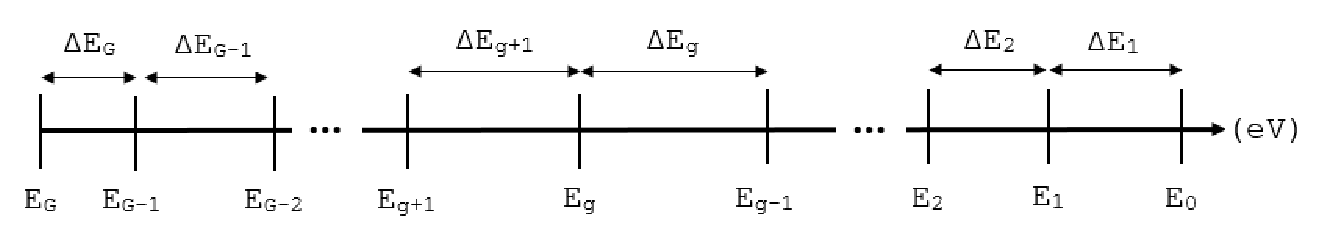
\includegraphics[width=1.00\textwidth]{figures/sec_Sn/MG_Energy_Bands.eps}
\caption{Interval structure of the multigroup methodology.}
\label{fig::Sn_MG_energy_bands}
\end{figure}

For the remainder of this energy discretization procedure, we will utilize the steady-state form of the transport equation in Eq. (\ref{eq::Sn_transport_eq_op_SS}). The time-dependent and eigenvalue forms are analagous and would be derived identically. Taking the energy interval for group $g$ as defined in Eq. (\ref{eq::Sn_MG_energy_interval}), the energy-integrated angular flux of group $g$ is

\begin{equation}
\label{eq::Sn_MG_ang_flux_g}
\Psi_g (\vec{r}, \vec{\Omega}) = \int_{E_g}^{E_{g-1}} \, \Psi (\vec{r}, E, \vec{\Omega}) \, dE .
\end{equation}

\noindent We can then use the energy-integrated angular flux to form the following coupled, $(g=1,...,G)$, discrete equations (we have dropped the spatial parameter and some of the angular parameters for further clarity):

\begin{equation}
\label{eq::Sn_MG_trans_eq}
\left(  \vec{\Omega} \cdot \vec{\nabla} + \sigma_{t,g}  \right) \Psi_g =  \sum_{g'=1}^{G} \left[ \frac{\chi_g}{4 \pi} \nu \sigma_{f,g'} \int_{4 \pi} \Psi_{g'} (\vec{\Omega}') \, d\Omega' + \int_{4 \pi} \sigma_{s}^{g' \rightarrow g} (\vec{\Omega}' , \vec{\Omega} ) \Psi_{g'} (\vec{\Omega}')  \, d\Omega'  \right] + Q_g
\end{equation}

\noindent where

\begin{equation}
\label{eq::Sn_MG_exact_condensed_terms}
\begin{aligned}
\sigma_{t,g} (\vec{r},\vec{\Omega}) & \equiv \frac{\int_{E_{g}}^{E_{g-1}} \sigma_{t} (\vec{r},\vec{\Omega},E) \Psi (\vec{r},\vec{\Omega}, E) \, dE}{\int_{E_{g}}^{E_{g-1}} \int_{4 \pi} \Psi (\vec{r},\vec{\Omega}, E) \, dE}\\
\nu\sigma_{f,g} (\vec{r}) & \equiv \frac{\int_{E_{g}}^{E_{g-1}} \nu\sigma_{f} (\vec{r},E)  \int_{4 \pi} \Psi (\vec{r},\vec{\Omega}, E) \, dE d\Omega}{\int_{E_{g}}^{E_{g-1}} \int_{4 \pi} \Psi (\vec{r},\vec{\Omega}, E) \, dE d\Omega} \\
\chi_g & \equiv \int_{E_{g}}^{E_{g-1}} \chi  (\vec{r},E) \, dE \\
\sigma_{s}^{g' \rightarrow g} (\vec{r},\vec{\Omega}' , \vec{\Omega} ) & \equiv \frac{\int_{E_{g'}}^{E_{g'-1}} \left[ \int_{E_{g}}^{E_{g-1}} \sigma_s (\vec{r},E' \rightarrow E,\vec{\Omega}' , \vec{\Omega} ) \, dE \right] \Psi (\vec{r},\vec{\Omega}', E') \, dE' }{\int_{E_{g}}^{E_{g-1}}  \Psi (\vec{r},\vec{\Omega}, E) \, dE} \\
Q_g (\vec{r}, \vec{\Omega}) & \equiv \int_{E_{g}}^{E_{g-1}} Q (\vec{r}, \vec{\Omega}, E) \, dE
\end{aligned}
\end{equation}

The above equations are mathematically exact to those presented in Eqs. (\ref{eq::Sn_transport_eq_full} - \ref{eq::Sn_transport_eq_op_SS}) and we have made no approximations at this time. However, this requires full knowledge of the energy distribution of the angular flux solution at all positions in our problem domain since we weight the multigroup cross sections with this solution. This is obviously impossible since the energy distibution is part of the solution space we are trying to solve for. Instead, we now define the process to make the multigroup discretization an effective approximation method.

We first define an approximate angular flux distribution for a region $s$:

\begin{equation}
\label{eq::Sn_MG_flux_approx}
\Psi (\vec{r},\vec{\Omega}, E) =  \hat{\Psi} (\vec{r},\vec{\Omega}) f_{s} (E) ,
\end{equation}

\noindent which is a factorization of the angular flux solution into a region-dependent energy function, $f_s (E)$, and a spatially/angularly dependent function, $\hat{\Psi} (\vec{r},\vec{\Omega})$. With this approximation, we can redefine the energy-collapsed cross sections of Eq. (\ref{eq::Sn_MG_exact_condensed_terms}):

\begin{equation}
\label{eq::MG_approx_condensed_terms}
\begin{aligned}
\sigma_{t,g} (\vec{r},\vec{\Omega}) & \equiv \frac{\int_{E_{g}}^{E_{g-1}} \sigma_{t} (\vec{r},\vec{\Omega},E) f_{s} (E) \, dE}{\int_{E_{g}}^{E_{g-1}} f_{s} (E) \, dE} ,\\
\nu\sigma_{f,g} (\vec{r}) & \equiv \frac{\int_{E_{g}}^{E_{g-1}} \nu\sigma_{f} (\vec{r},E)  f_{s} (E) \, dE }{\int_{E_{g}}^{E_{g-1}} f_{s} (E) \, dE}, \\
\sigma_{s}^{g' \rightarrow g} (\vec{r},\vec{\Omega}' , \vec{\Omega} ) & \equiv \frac{\int_{E_{g'}}^{E_{g'-1}} \left[ \int_{E_{g}}^{E_{g-1}} \sigma_s (\vec{r},E' \rightarrow E,\vec{\Omega}' , \vec{\Omega} ) \, dE \right] f_{s} (E')\, dE' }{\int_{E_{g}}^{E_{g-1}}  f_{s} (E) \, dE} .
\end{aligned}
\end{equation}

\noindent It is noted that we do not need to redefine the fission spectrum or the distributed external sources since they are not weighted with the angular flux solution. With this energy factorization, we would expect, in general, that the approximation error will tend to zero as the number of discrete energy groups increases (thereby making the energy bins thinner). This is especially true if the group structure is chosen with many more bins in energy regions with large variations in the energy solution. For certain problems, the region-dependent energy function is well understood ({\em i.e.} almost exactly known). This means, that for these problems, we can achieve reasonable solution accuracy with only a few groups where the energy bins of the multigroup discretization are well chosen.

%%%%%%%%%%%%%%%%%%%%%%%%%%%%%%%%%%%%%%%%%%%%%%%%%%%
%%%   Section - Angle Discretization
\section{Angular Discretization}
\label{sec::Sn_Angle}

Now that we have provided the discretization of the energy variable, we next focus on the discretization of the transport problem in angle. We will do this in two stages: 1) expand the scattering source and the distributed external source in spherical harmonics and 2) collocate the angular flux at the interpolation points of the angular trial space. We will perform these discretization procedures by taking the stready-state equation presented in Eq. (\ref{eq::Sn_transport_eq_op_SS}), dropping spatial parameterization, combining the fission and external sources into a single term, and using only 1 energy group:

\begin{equation}
\label{eq::Sn_Angle_simple_trans_eq}
\vec{\Omega} \cdot \vec{\nabla} \Psi (\vec{\Omega}) + \sigma_t \Psi (\vec{\Omega}) = \int_{4 \pi}  d\Omega' \, \sigma_s ( \vec{\Omega}' \rightarrow \vec{\Omega}) \Psi (\vec{\Omega}') + Q  (\vec{\Omega}) .
\end{equation}

We first develop an approximation for the scattering term in Eq. (\ref{eq::Sn_Angle_simple_trans_eq}) by expanding the angular flux and the scattering cross section in spherical harmonics functions and Legendre polynomials, respectively. We begin by first assuming that the material is isotropic in relation to the radiation's initial direction. From this assumption, the parameterization of the scattering cross section can be written in terms of only the scattering angle, $\mu_0$,

\begin{equation}
\label{eq::Sn_scatt_xs}
\sigma_s ( \vec{\Omega}' \rightarrow \vec{\Omega}) = \frac{1}{2 \pi} \sigma_s ( \vec{\Omega}' \cdot \vec{\Omega}) = \frac{1}{2 \pi} \sigma_s ( \mu_0) , 
\end{equation}

\noindent where $\mu_0 \equiv  \vec{\Omega}' \cdot \vec{\Omega}$. With this simplification, the scattering cross section can now be expanded in an infinite series in terms of the Legendre polynomials,

\begin{equation}
\label{eq::Sn_scatt_xs_legendre}
\sigma_s ( \vec{\Omega}' \rightarrow \vec{\Omega}) = \sum\displaylimits_{p=0}^{\infty} \frac{2p + 1}{4 \pi}  \sigma_{s,p} P_p ( \mu_0) , 
\end{equation}

\noindent where $\sigma_{s,p}$ is the $p$ angular moment of the scattering cross section. These angular moments of the scattering cross section have the form:

\begin{equation}
\label{eq::Sn_scatt_xs_moments}
	\sigma_{s,p} \equiv  \int_{-1}^{1} \, d \mu_0 \, \sigma_s ( \mu_0) P_p (\mu_0)  .
\end{equation}

With the scattering cross section redefined, we can now expand the angular flux in terms of an infinite series of the spherical harmonics functions, $Y$,

\begin{equation}
\label{eq::Sn_ang_flux_sph_harm_funcs}
\Psi (\vec{\Omega}) = \frac{1}{4 \pi} \sum\displaylimits_{k=0}^{\infty} \sum\displaylimits_{n=-k}^{k} \Phi_{k,n} Y_{k,n} (\vec{\Omega})
\end{equation}

\noindent where the angular moments of the angular flux, $\Phi_{k,n}$, have the form:

\begin{equation}
\label{eq::Sn_flux_moments}
	\Phi_{k,n} \equiv \int_{4 \pi} d\Omega \, \Psi(\vec{\Omega}) \, Y_{p,n} (\vec{\Omega}).
\end{equation}

\noindent We note that the $p$ and $k$ orders of the scattering cross section and angular flux expansions, respectively, are not corresponding. We then take the scattering cross section expansion of Eq. (\ref{eq::Sn_scatt_xs_legendre}) and the angular flux expansion of Eq. (\ref{eq::Sn_ang_flux_sph_harm_funcs}), and insert them into the original scattering term of the right-hand-side of Eq. (\ref{eq::Sn_Angle_simple_trans_eq}). After significant algebra and manipulations, which we will not include here for brevity, the scattering term can be greatly simplified (the full details of this are located in Appendix \ref{sec::appendix_SN}). Eq. (\ref{eq::Sn_Angle_simple_trans_eq}) can now be written again with this alternate and simplified scattering term that is composed of the cross section and angular flux moments:

\begin{equation}
\label{eq::Sn_Angle_simple_trans_eq_w_moments_inf}
\vec{\Omega} \cdot \vec{\nabla} \Psi (\vec{\Omega}) + \sigma_t \Psi (\vec{\Omega}) = \sum_{p=0}^{\infty} \frac{2p + 1}{4 \pi} \sigma_{s,p}   \sum_{n=-p}^{p}  \Phi_{p,n}  Y_{p,n} (  \vec{\Omega} )+ Q  (\vec{\Omega}) .
\end{equation}

From the initial assumption of material isotropy (which may or not be an approximation), the scattering term of Eq. (\ref{eq::Sn_Angle_simple_trans_eq_w_moments_inf}) has introduced no approximation. Unfortunately, this form requires an infinite series expansion which we cannot use with only finite computational resources. Instead, we truncate the series at some maximum expansion order, $N_p$, which, in general, introduces an approximate form for the scattering. However, we note that if the problem scattering can be exactly captured with moments through order $N_p$, then we have introduced no approximation with this truncation. With this order of truncation, we again write the angularly continuous Eq. (\ref{eq::Sn_Angle_simple_trans_eq_w_moments_inf}), but also fold the source term into the spherical harmonics expansion,

\begin{equation}
\label{eq::Sn_Angle_simple_trans_eq_w_moments_trunc}
\vec{\Omega} \cdot \vec{\nabla} \Psi (\vec{\Omega}) + \sigma_t \Psi (\vec{\Omega}) = \sum_{p=0}^{N_p} \frac{2p + 1}{4 \pi}   \sum_{n=-p}^{p}   Y_{p,n} (  \vec{\Omega} ) \left[ \sigma_{s,p} \Phi_{p,n} + Q_{p,n}  \right] .
\end{equation}

At this point, one may wonder why we have alterred the scattering operator so that it is terms of moments of the scattering cross sections and the angular flux. The reason is two-fold which will also be discussed in further detail later in this chapter. First, it greatly reduces the phase space of the scattering cross sections. With proper preprocessing, the scattering cross sections can be simplified into just their Legendre moments, instead of having to store angle-to-angle quantities ($\vec{\Omega}' \rightarrow \vec{\Omega}$). For every group-to-group combination in energy ($g' \rightarrow g$), there are only the $N_p$ moments of the scattering cross section. Secondly, the contribution of the angular flux into the scattering source with its moments can also greatly reduce the dimensional space that needs to be stored in computer memory. This will be discussed later in further detail in Section \ref{sec::Sn_Solution_Iterative}, but it simply means that we only have to store $N_{mom}$ angular flux moments for use in the scattering source. In 1 dimension, $N_{mom}$ is equal to ($N_p + 1$). In 2 dimensions, $N_{mom}$ is equal to $\frac{(N_p + 1) (N_p + 2)}{2}$. In 3 dimensions, $N_{mom}$ is equal to $(N_p + 1)^2$. For comparative purposes, we have plotted $N_{mom}$ for 1,2, and 3 dimensions up to order 8 in Figure \ref{fig::Sn_Num_Sph_Harm_Moments}.

\begin{figure}
\centering
\includegraphics[width=0.65\textwidth]{figures/sec_Sn/Num_Sph_Harm_Moments.eps}
\caption[Number of spherical harmonics moments]{Number of spherical harmonics moments, $N_{mom}$, in 1D, 2D, and 3D as a function of the expansion order, $p$.}
\label{fig::Sn_Num_Sph_Harm_Moments}
\end{figure}

Up to this point, we have only presented the methodology to express our source terms with expansions of the spherical harmonics functions. Next, we describe the second portion of our angular discretization by deriving the standard $S_N$ equations using a collocation technique. We begin by choosing a set of $M$ distinct points and weights to form a quadrature set in angular space: $\{  \vec{\Omega}_m, w_m \}_{m=1}^M$. We will give further details about the required characteristics of this quadrature set as well as a couple of common options a little later. Using this quadrature set, we can further define a trial space for the angular flux,

\begin{equation}
\label{eq::Sn_ang_flux_basis}
\Psi (\vec{\Omega}) = \sum\displaylimits_{m=1}^{M} B_m (\vec{\Omega})  \Psi_m ,
\end{equation}

\noindent where the angular bases, $B_m$, satisfy the {\em Kronecker} property,

\begin{equation}
\label{eq::Sn_ang_basis_kroneker}
 B_j (\vec{\Omega}_m) = \delta_{j,m}, 
\end{equation}

\noindent as well as the {\em Lagrange} property,

\begin{equation}
\label{eq::Sn_ang_basis_lagrange}
\sum\displaylimits_{m=1}^{M} B_m (\vec{\Omega}_m) = 1  ,
\end{equation}

\noindent and the singular value of the angular flux along a given direction has the following notation:

\begin{equation}
\label{eq::Sn_ang_flux_identity}
\Psi_m = \Psi (\vec{\Omega}_m).
\end{equation}

Next, we substitute Eq. (\ref{eq::Sn_ang_flux_basis}) into Eq. (\ref{eq::Sn_Angle_simple_trans_eq_w_moments_trunc}), drop the external source for clarity, and collocate at the ($k=1,...,M$) interpolation (quadrature) points,

\begin{equation}
\label{eq::Sn_Angle_simple_trans_eq_w_ang_basis}
\begin{aligned}
\vec{\Omega} \cdot \vec{\nabla} \left( \sum\displaylimits_{m=1}^{M} B_m (\vec{\Omega}_k)  \Psi_m \right) + \sigma_t \left(  \sum\displaylimits_{m=1}^{M} B_m (\vec{\Omega}_k)  \Psi_m \right) \\
= \sum_{p=0}^{N_p} \frac{2p + 1}{4 \pi} \sigma_{s,p}   \sum_{n=-p}^{p}   Y_{p,n} (  \vec{\Omega} ) \left(  \sum\displaylimits_{m=1}^M \Psi_m \int_{4 \pi} d\Omega \, B_m (\vec{\Omega}_k)  \, Y_{p,n} (\vec{\Omega})  \right)  \\
k=1,...,M
\end{aligned} ,
\end{equation}

\noindent where we inserted Eq. (\ref{eq::Sn_ang_flux_basis}) into Eq. (\ref{eq::Sn_flux_moments}) to form a slightly modified form for the angular flux moments:

\begin{equation}
\label{eq::Sn_flux_mom_int_w_basis}
\Phi_{p,n} = \sum\displaylimits_{m=1}^M \Psi_m \int_{4 \pi} d\Omega \, B_m (\vec{\Omega})  \, Y_{p,n} (\vec{\Omega}).
\end{equation}

\noindent The {\em Kronecker} property of Eq. (\ref{eq::Sn_ang_basis_kroneker}), is then used at the collocation points so that Eq. (\ref{eq::Sn_Angle_simple_trans_eq_w_ang_basis}) can be simplified into the following form (where we have reintroduced the distributed source term in terms of its contribution for angle $m$):

\begin{equation}
\label{eq::Sn_trans_eq_angle_disc_FINAL}
\begin{aligned}
\vec{\Omega}_m \cdot \vec{\nabla} \Psi_{m}  + \sigma_{t}   \Psi_{m}=  \sum_{p=0}^{N_P} \frac{2p + 1}{4 \pi}  \sigma_{s,p}  \sum_{n=-p}^{p}  Y_{p,n} (  \vec{\Omega}_m )  \Phi_{p,n}  + Q_{m}  \\
m=1,...,M
\end{aligned} .
\end{equation}

Equation (\ref{eq::Sn_trans_eq_angle_disc_FINAL}) represents the transport equation that has been discretized into $M$ separate equations in angle (for 1 energy group and no spatial discretization). Up to this point, we have simply stated that there is some angular quadrature set composed of $M$ directions and weights that will satisfy some conditions of the solution, but we have not explicitly stated these conditions. For this work we will require our angular quadrature set to maintain the following properties:

\begin{enumerate}
\item The weights can sum to 1 by some normalization procedure: $\sum\displaylimits_m w_m = 1$.
\item The odd angular moments sum to $\vec{0}$: $\sum\displaylimits_m w_m \left( \vec{\Omega}_m  \right)^n =  \vec{0}$ ($n=1,3,5,...$).
\item $\sum\displaylimits_m w_m  \vec{\Omega}_m \vec{\Omega}_m = \frac{1}{3} \mathbb{I}  $, where $\mathbb{I}$ is the identity tensor.
\item The points and weights are symmetric about the primary axes in angular space. 
\item The points and weights also need to have symmetry about the problem domain boundary (this is not an issue if the domain is a rectangle in 2D or an orthogonal parallelepiped in 3D). This point is important for reflecting boundary conditions and is described in greater detail in Section \ref{sec::Sn_BC}.
\end{enumerate}

\noindent Point 4 requires some additional explanation. In 1 dimension, this corresponds to symmetry about the point 0 on the interval $[-1, 1]$. In 2 dimensions, this corresponds to quadrant-to-quadrant symmetry about the x-y primary axes of the unit circle. In 3 dimensions, this corresponds to octant-to-octant symmetry about the x-y-z primary axes of the unit sphere. 

From these properties, especially property 4, our 2D and 3D quadrature sets can be constructed in a simple and consistent manner (1D quadrature sets have different construction and our work does not include them). For both 2D and 3D problems, we can generate a subset of the quadrature points and weights on a single octant of the unit sphere, where each quadrature point in this subset has the form: $\vec{\Omega} = [\mu, \eta , \xi]$ . If we are solving a 2D problem, we would then project the quadrature points onto the $(0 < \theta < \frac{\pi}{2})$ portion of the unit circle so that they have the form: $\vec{\Omega} = [\mu, \eta ]$ (we can then view the primary octant as the primary quadrant). Once we have defined the quadrature points and weights for the primary quadrant or octant, we can then directly calculate the remainder of the quadrature set by mapping to the other quadrants or octants. Table \ref{tab::Sn_2D_octant_mapping} presents the mapping from the primary quadrant to the other 3 quadrants for 2D problems. Table \ref{tab::Sn_3D_octant_mapping} presents the mapping from the primary octant to the other 7 octants for 3D problems. In these tables, the `1' subscript corresponds to those angles generated in the primary quadrant or octant.

\begin{table}[hbt]
\centering
\caption{2D angle mapping from the first quadrant into the other 3 quadrants.}
\begin{tabular}{|c|cc|}
	\hline
	Quadrant & $\mu$ & $\eta$ \\
	\hline
	1 & $\mu_1=\mu_1$ & $\eta_1=\eta_1$ \\
	\hline
	2 & $\mu_2=-\mu_1$ & $\eta_2=\eta_1$ \\
	\hline
	3 & $\mu_3=-\mu_1$ & $\eta_3=-\eta_1$ \\
	\hline
	4 & $\mu_4=\mu_1$ & $\eta_4=-\eta_1$ \\
	\hline
\end{tabular}
\label{tab::Sn_2D_octant_mapping}
\end{table}

\begin{table}[hbt]
\centering
\caption{3D angle mapping from the first octant into the other 7 octants.}
\begin{tabular}{|c|ccc|}
	\hline
	Octant & $\mu$ & $\eta$ & $\xi $ \\
	\hline
	1 & $\mu_1=\mu_1$ & $\eta_1=\eta_1$ & $\xi_1=\xi_1$ \\
	\hline
	2 & $\mu_2=-\mu_1$ & $\eta_2=\eta_1$ & $\xi_2=\xi_1$ \\
	\hline
	3 & $\mu_3=-\mu_1$ & $\eta_3=-\eta_1$ & $\xi_3=\xi_1$ \\
	\hline
	4 & $\mu_4=\mu_1$ & $\eta_4=-\eta_1$ & $\xi_4=\xi_1$ \\
	\hline
	5 & $\mu_5=\mu_1$ & $\eta_5=\eta_1$ & $\xi_5=-\xi_1$ \\
	\hline
	6 & $\mu_6=-\mu_1$ & $\eta_6=\eta_1$ & $\xi_6=-\xi_1$ \\
	\hline
	7 & $\mu_7=-\mu_1$ & $\eta_7=-\eta_1$ & $\xi_7=-\xi_1$ \\
	\hline
	8 & $\mu_8=\mu_1$ & $\eta_8=-\eta_1$ & $\xi_8=-\xi_1$ \\
	\hline
\end{tabular}
\label{tab::Sn_3D_octant_mapping}
\end{table}

We conclude our discussion of angular discretizations by presenting two common angular quadrature sets that will be employed in this dissertation work. Section \ref{sec::Sn_Angle_LS} presents the Level Symmetric (LS) quadrature set and Section \ref{sec::Sn_Angle_PGLC} presents the Product Gauss-Legendre-Chebyshev (PGLC) quadrature set. Both of these quadrature sets can be formed from the procedure outlined before: form the primary octant and then map appropriately.

%%%%%%%%%%%%%%%%%%%%%%%%%%%%%%%%%%%%%%%%%%%%%%%%%%%
%%%   SubSection - Level-Symmetric
\subsection{Level Symmetric Quadrature Set}
\label{sec::Sn_Angle_LS}

The first quadrature set we present is the common Level Symmetric set that has had extensive use in the radiation transport community \cite{lewis1984computational,carlson1968computing}. Its defining characteristic is the restriction that it is rotationally symmetric (invariant) about all three axes of the primary octant. This leads to a two-fold additional set of restrictions: 1) once the location of the first ordinate is selected, then all other ordinates are known; and 2) the weights can become negative. This negativity of the weights can be problematic and lead to unphysical solutions if the angular flux is not sufficiently smooth.

\begin{figure}
\centering
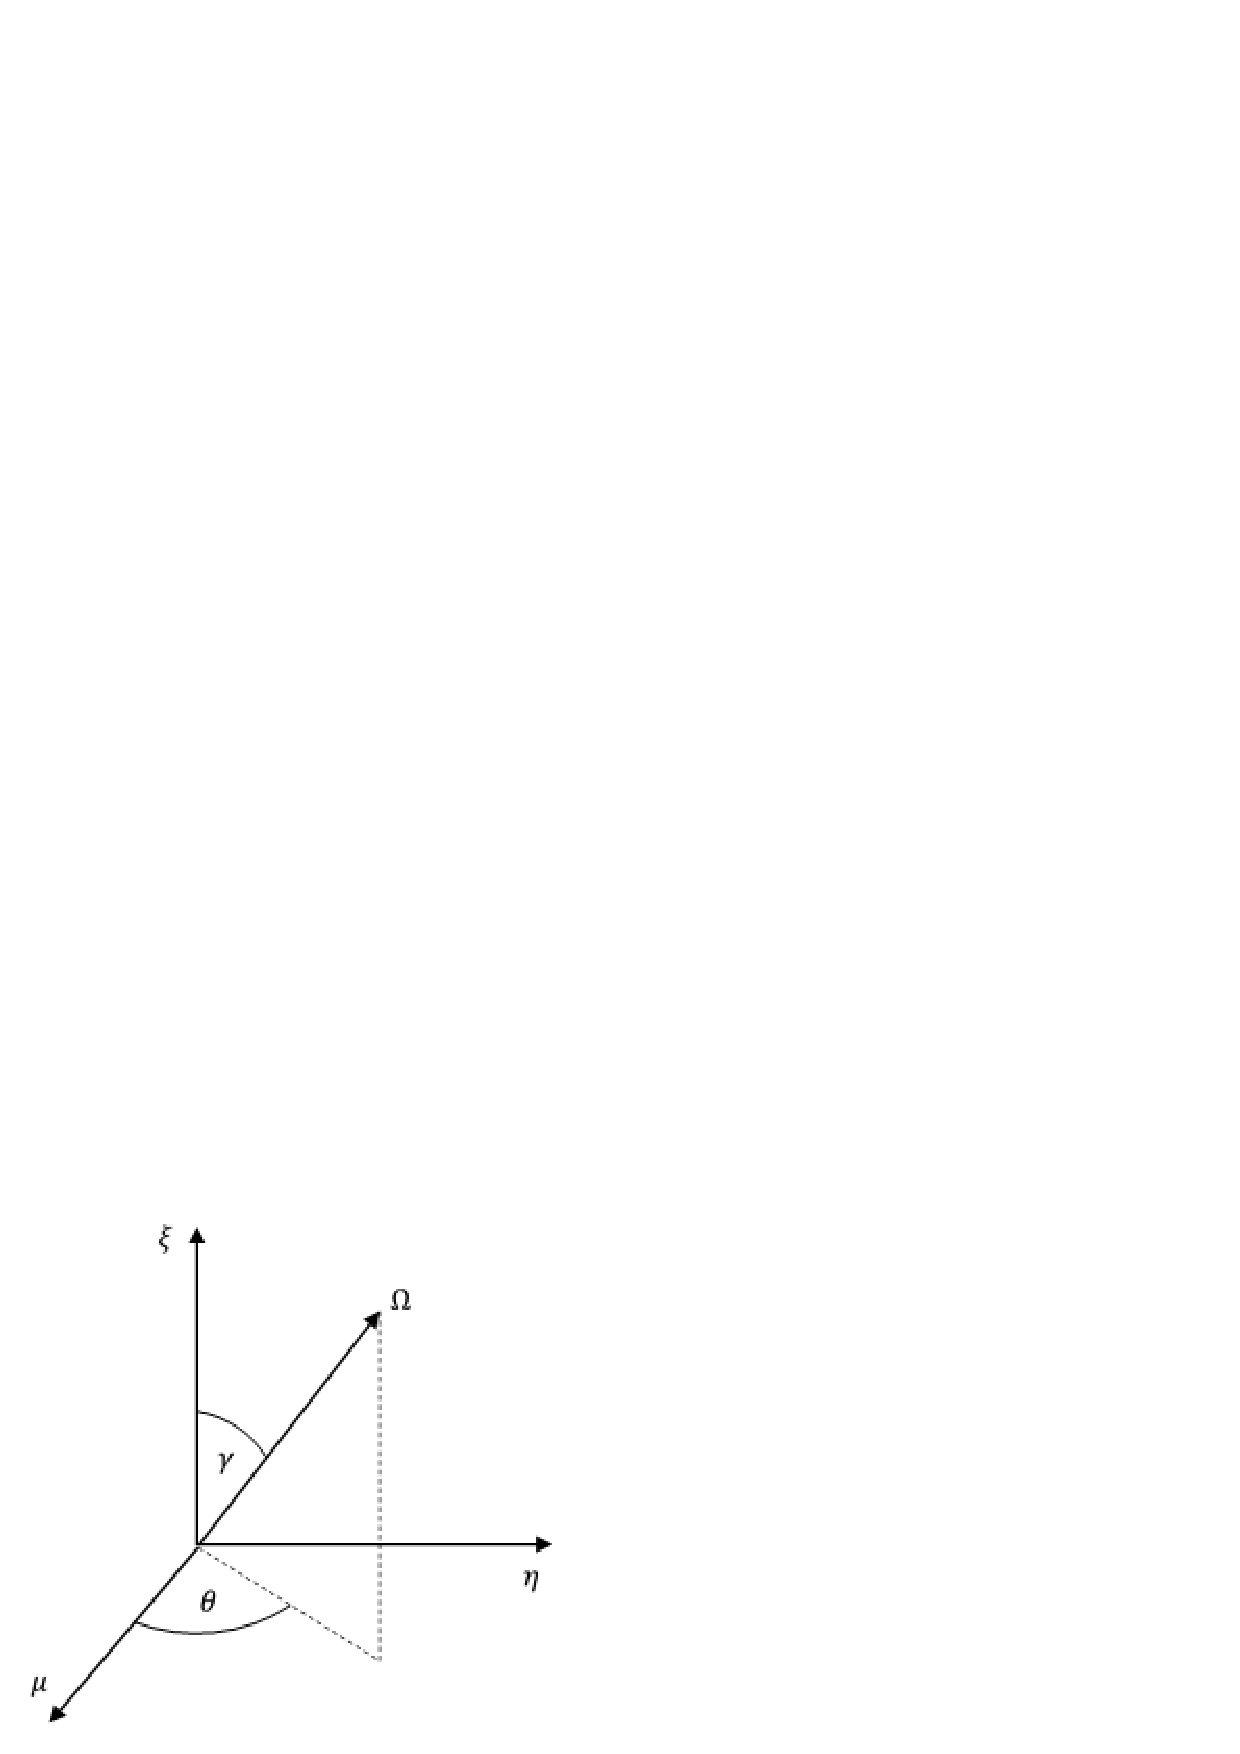
\includegraphics[width=0.45\textwidth]{figures/sec_Sn/Ang_Quad_Coord_Sys.png}
\caption[Angular Coordinate System]{Angular coordinate system for the direction $\vec{\Omega}$.}
\label{fig::Ang_Coord_Sys}
\end{figure}

We begin our description of the LS quadrature by analyzing the 3D angular coordinate system for a particular direction, $\vec{\Omega}$, as depicted in Figure \ref{fig::Ang_Coord_Sys}. The angular direction, $\vec{\Omega} = [\vec{\Omega}_x, \vec{\Omega}_y, \vec{\Omega}_z]$, is typically described with its directional cosines: $\mu$, $\eta$, and $\xi$. These are described by the angles $\theta$ and $\gamma$ of the coordinate system and allow us to give a functional form for each direction component:

\begin{equation}
\label{eq::Sn_Angle_angle_components}
\begin{aligned}
\vec{\Omega}_x =& \mu = \cos (\theta) \sin (\gamma)  =\cos (\theta)  \sqrt{1 - \xi^2}  \\
\vec{\Omega}_x =& \eta = \sin (\theta) \sin (\gamma)  =\sin (\theta)   \sqrt{1 - \xi^2}   \\
\vec{\Omega}_y =& \xi = \cos (\gamma)
\end{aligned} .
\end{equation}

\noindent The direction cosines are related and necessarily must have a Euclidean norm of 1:

\begin{equation}
\label{eq::Sn_Angle_angle_cos_relation}
\mu^2 + \eta^2 + \xi^2 = 1 .
\end{equation}

We conclude this discussion of the LS quadrature set with some examples. Figure \ref{fig::Sn_Angle_LS_Quads_3D} provides a visual depiction of the LS nodes and weights in the primary octant for varying orders. The magnitude of the weights are characterized by the relative size of the nodes. Figure \ref{fig::Sn_Angle_LS_Quads_2D} then provides the projection of the 3D LS quadrature set onto to the unit circle for various orders for use in 2D problems. We have included the full quadrature set in this image including the quadrant-to-quadrant mapping. 

\begin{figure}
\centering
	\begin{subfigure}[b]{0.48\textwidth}
		\centering
		\includegraphics[width=0.92\textwidth]{figures/sec_Sn/LS2_3D.eps}
		\caption{}
	\end{subfigure}
	\hfill
	\begin{subfigure}[b]{0.48\textwidth}
		\centering
		\includegraphics[width=0.92\textwidth]{figures/sec_Sn/LS4_3D.eps}
		\caption{}
	\end{subfigure}
	\vfill
	\begin{subfigure}[b]{0.48\textwidth}
		\centering
		\includegraphics[width=0.92\textwidth]{figures/sec_Sn/LS8_3D.eps}
		\caption{}
	\end{subfigure}
	\hfill
	\begin{subfigure}[b]{0.48\textwidth}
		\centering
		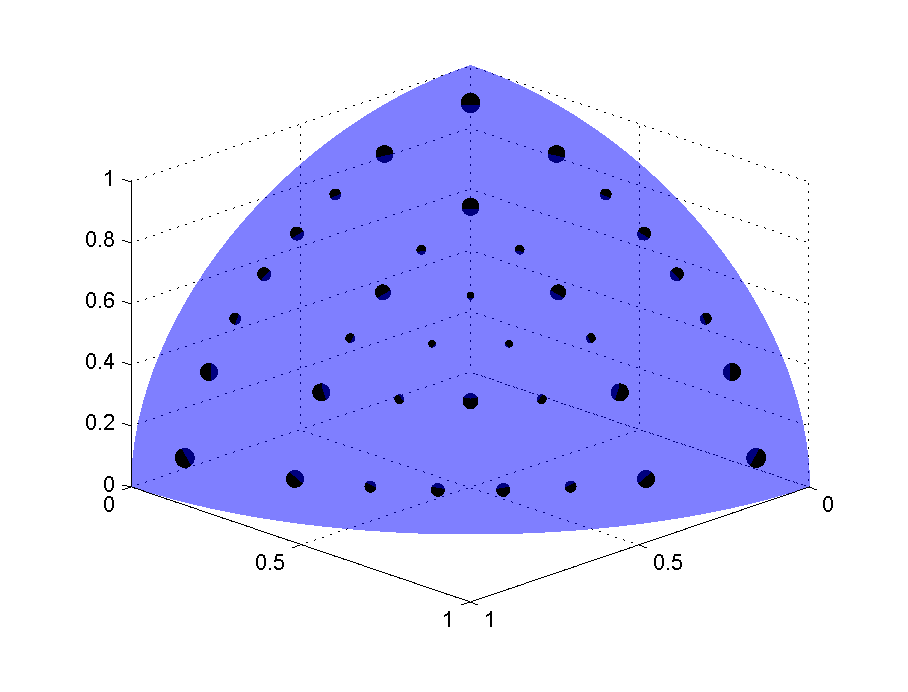
\includegraphics[width=0.92\textwidth]{figures/sec_Sn/LS16_3D.eps}
		\caption{}
	\end{subfigure}
\caption[3D Level-Symmetric angular quadrature set]{Level-Symmetric angular quadrature sets of order (a) 2, (b) 4, (c) 8, and (d) 16.}
\label{fig::Sn_Angle_LS_Quads_3D}
\end{figure}

\begin{figure}
\centering
	\begin{subfigure}[b]{0.48\textwidth}
		\centering
		\includegraphics[width=0.92\textwidth]{figures/sec_Sn/LS2_2D.eps}
		\caption{}
	\end{subfigure}
	\hfill
	\begin{subfigure}[b]{0.48\textwidth}
		\centering
		\includegraphics[width=0.92\textwidth]{figures/sec_Sn/LS4_2D.eps}
		\caption{}
	\end{subfigure}
	\vfill
	\begin{subfigure}[b]{0.48\textwidth}
		\centering
		\includegraphics[width=0.92\textwidth]{figures/sec_Sn/LS8_2D.eps}
		\caption{}
	\end{subfigure}
	\hfill
	\begin{subfigure}[b]{0.48\textwidth}
		\centering
		\includegraphics[width=0.92\textwidth]{figures/sec_Sn/LS16_2D.eps}
		\caption{}
	\end{subfigure}
\caption[2D Level-Symmetric angular quadrature set]{Projection of the 3D Level-Symmetric angular quadrature set with orders (a) 2, (b) 4, (c) 8, and (d) 16 onto the x-y space on the unit circle.}
\label{fig::Sn_Angle_LS_Quads_2D}
\end{figure}

%%%%%%%%%%%%%%%%%%%%%%%%%%%%%%%%%%%%%%%%%%%%%%%%%%%
%%%   SubSection - PGLC
\subsection{Product Gauss-Legendre-Chebyshev Quadrature Set}
\label{sec::Sn_Angle_PGLC}

The second angular quadrature set we will present is a Product Gauss-Legendre-Chebyshev (PGLC) set \cite{abu1977compatible}. It is formed by the product-wise multiplication of a Gauss-Chebyshev quadrature in the azimuthal direction and a Gauss-Legendre quadrature in the polar direction. It has the following key differences from the Level Symmetric set:

\begin{itemize}
	\item Does not have $90^o$ rotational invariance within the primary octant; still maintains octant-to-octant symmetry however;
	\item Has more control over the placement of the anglular directions within the primary octant;
	\item Quadrature weights are aligned with the polar level;
	\item Has strictly positive weights for all polar and azimuthal combinations.
\end{itemize}

From the listed differences, we can already discern some clear advantages and disadvantages from a fully-symmetric quadrature set like LS. If a high number of angles are required for a problem, then negative weights do not arise. This is beneficial for transport problems with significant discontinuities. Also, the quadrature directions can be preferentially distributed in the primary octant if required for a particular problem. For example, if the transport solution is smoothly varying in the polar direction and not in the azimuthal direction, then we can specify a larger number of quadrature points in the azimuthal direction, with much fewer points in the polar direction. However, this also highlights the fact that the quadrature weights are aligned with the polar level, which can lead to less accurate moment integrations for certain transport problems. 

For this dissertation, we will use the following notation to define the product nature of the PGLC quadrature points: $S_{a}^{p}$. Here, $a$ and $p$ correspond to the number of azimuthal and polar directions in the primary octant, respectively. We demonstrate this definition in Figure \ref{fig::Sn_Angle_PGLC_Quads_3D} for the primary octant with several combinations of azimuthal and polar directions. Figure \ref{fig::Sn_Angle_PGLC_Quads_2D} then presents the projections of these quadrature sets onto the unit circle for use in 2D transport problems. Again, the size of the direction marker corresponds to the relative weight of quadrature point. One can clearly see that the weights vary on the polar levels and all azimuthal weights on a given polar level are constant.

\begin{figure}
\centering
	\begin{subfigure}[b]{0.48\textwidth}
		\centering
		\includegraphics[width=0.92\textwidth]{figures/sec_Sn/PGLC2_2_3D.png}
		\caption{}
	\end{subfigure}
	\hfill
	\begin{subfigure}[b]{0.48\textwidth}
		\centering
		\includegraphics[width=0.92\textwidth]{figures/sec_Sn/PGLC2_4_3D.png}
		\caption{}
	\end{subfigure}
	\vfill
	\begin{subfigure}[b]{0.48\textwidth}
		\centering
		\includegraphics[width=0.92\textwidth]{figures/sec_Sn/PGLC4_2_3D.png}
		\caption{}
	\end{subfigure}
	\hfill
	\begin{subfigure}[b]{0.48\textwidth}
		\centering
		\includegraphics[width=0.92\textwidth]{figures/sec_Sn/PGLC4_4_3D.png}
		\caption{}
	\end{subfigure}
	\vfill
	\begin{subfigure}[b]{0.48\textwidth}
		\centering
		\includegraphics[width=0.92\textwidth]{figures/sec_Sn/PGLC6_6_3D.png}
		\caption{}
	\end{subfigure}
	\hfill
	\begin{subfigure}[b]{0.48\textwidth}
		\centering
		\includegraphics[width=0.92\textwidth]{figures/sec_Sn/PGLC8_8_3D.png}
		\caption{}
	\end{subfigure}
\caption[3D Product Gauss-Legendre-Chebyshev angular quadrature set]{Product Gauss-Legendre-Chebyshev angular quadrature set with orders: (a) S$_2^2$, (b) S$_2^4$, (c) S$_4^2$, (d) S$_4^4$, (e) S$_6^6$, and (f) S$_8^8$.}
\label{fig::Sn_Angle_PGLC_Quads_3D}
\end{figure}

\begin{figure}
\centering
	\begin{subfigure}[b]{0.46\textwidth}
		\centering
		\includegraphics[width=0.85\textwidth]{figures/sec_Sn/PGLC2_2_2D.eps}
		\caption{}
	\end{subfigure}
	\hfill
	\begin{subfigure}[b]{0.46\textwidth}
		\centering
		\includegraphics[width=0.85\textwidth]{figures/sec_Sn/PGLC2_4_2D.eps}
		\caption{}
	\end{subfigure}
	\vfill
	\begin{subfigure}[b]{0.46\textwidth}
		\centering
		\includegraphics[width=0.85\textwidth]{figures/sec_Sn/PGLC4_2_2D.eps}
		\caption{}
	\end{subfigure}
	\hfill
	\begin{subfigure}[b]{0.46\textwidth}
		\centering
		\includegraphics[width=0.85\textwidth]{figures/sec_Sn/PGLC4_4_2D.eps}
		\caption{}
	\end{subfigure}
	\vfill
	\begin{subfigure}[b]{0.46\textwidth}
		\centering
		\includegraphics[width=0.85\textwidth]{figures/sec_Sn/PGLC6_6_2D.eps}
		\caption{}
	\end{subfigure}
	\hfill
	\begin{subfigure}[b]{0.46\textwidth}
		\centering
		\includegraphics[width=0.85\textwidth]{figures/sec_Sn/PGLC8_8_2D.eps}
		\caption{}
	\end{subfigure}
\caption[2D Product Gauss-Legendre-Chebyshev angular quadrature set]{Projection of the 3D Product Gauss-Legendre-Chebyshev angular quadrature set with orders: (a) S$_2^2$, (b) S$_2^4$, (c) S$_4^2$, (d) S$_4^4$, (e) S$_6^6$, and (f) S$_8^8$ onto the x-y space on the unit circle.}
\label{fig::Sn_Angle_PGLC_Quads_2D}
\end{figure}

%%%%%%%%%%%%%%%%%%%%%%%%%%%%%%%%%%%%%%%%%%%%%%%%%%%
%%%   Section - Boundary Conditions
\section{Boundary Conditions}
\label{sec::Sn_BC}

Using the energy and angular discretizations presented in Sections \ref{sec::Sn_MG} and \ref{sec::Sn_Angle}, respectively, we write the standard, steady-state, multigroup $S_N$ transport equation for one angular direction, $m$, and one energy group, $g$:

\begin{equation}
\label{eq::Sn_mg_sn_trans_eq}
\begin{aligned}
	 \left( \vec{\Omega}_m \cdot \vec{\nabla}  + \sigma_{t,g}  \right)  \Psi_{m,g}= \sum_{g'=1}^{G} \sum_{p=0}^{N_P} \frac{2p + 1}{4 \pi} \sigma_{s,p}^{g' \rightarrow g}   \sum_{n=-p}^{p}  \Phi_{p,n,g'}  Y_{p,n} (  \vec{\Omega}_m )  \\
	+ \frac{\chi_g}{4 \pi} \sum_{g'=1}^{G} \nu \sigma_{f,g'} \Phi_{g'}   + Q_{m,g}
\end{aligned} , 
\end{equation}

\noindent where we have dropped the spatial parameter for clarity and is beholden to the following general, discretized boundary condition:

\begin{equation}
\label{eq::Sn_mg_sn_trans_eq_bc}
\Psi_{m,g} (\vec{r}) = \Psi^{inc}_{m,g} (\vec{r}) + \sum_{g'=1}^{G} \sum_{\vec{\Omega}_{m'} \cdot \vec{n} > 0} \gamma_{g' \rightarrow g}^{m' \rightarrow m} (\vec{r})  \Psi_{m',g'} (\vec{r})  .
\end{equation}

\noindent These $(M \text{x} G)$ number of discrete, tightly-coupled equations are currently defined as continuous in space.

For this dissertation work, we will consider only one type of boundary conditions: Dirichlet-type boundaries (also called {\em first-type boundary condition} in some physics and mathematical communities). In particular we will only utilize incoming-incident and reflecting boundary conditions which correspond to $\vec{r} \in \partial \mathcal{D}^d$ and $\vec{r} \in \partial \mathcal{D}^r$, respectively. The full domain boundary is then the union: $\partial \mathcal{D} = \partial \mathcal{D}^d \cup \partial \mathcal{D}^r$. This leads to the boundary condition being succinctly written for one angular direction, $m$, and one energy group, $g$ as

\begin{equation}
\label{eq::Sn_simple_BC}
\Psi_{m,g} (\vec{r}) = \begin{cases}
	\Psi^{inc}_{m,g} (\vec{r}) , & \vec{r} \in \partial \mathcal{D}^d \\
	\Psi_{m',g} (\vec{r}) , & \vec{r} \in \partial \mathcal{D}^r
\end{cases}
\end{equation}

\noindent where the reflecting angle is $\vec{\Omega}_{m'} = \vec{\Omega}_{m} - 2 \left(  \vec{\Omega}_{m} \cdot \vec{n} \right) \vec{n}$ and $\vec{n}$ is oriented outward from the domain. To properly utilize the reflecting boundary condition that we have proposed, the angular quadrature set defined in Section \ref{sec::Sn_Angle} needs the following properties.

\begin{enumerate}
 	\item The reflected directions, $\vec{\Omega}_{m'}$, are also in the quadrature set for all $\vec{r} \in \partial \mathcal{D}^r$.
	\item The weights of the incident, $w_m$, and reflected, $w_{m'}$, angles must be equal.
\end{enumerate} 

\noindent For problems where the reflecting boundaries align with the $x,y,z$ axes, this will not be an issue with standard quadrature sets ({\em e.g.} level-symmetric or Gauss-Legendre-Chebyshev). However, if the reflecting boundaries do not align in this manner, then additional care must be employed in calculating appropriate angular quadrature sets.

%%%%%%%%%%%%%%%%%%%%%%%%%%%%%%%%%%%%%%%%%%%%%%%%%%%
%%%   Section - Spatial Discretization
\section{Spatial Discretization}
\label{sec::Sn_Spatial}

For the spatial discretization of the problem domain, we simplify Eq. (\ref{eq::Sn_mg_sn_trans_eq}) into a single energy group and drop the fission term (it can be lumped into the 0th order external source term and will act similarly to the total interaction term)

\begin{equation}
\label{eq::Sn_trans_eq_simple_no_energy_groups}
\vec{\Omega}_m \cdot \vec{\nabla} \Psi_{m}  + \sigma_{t}   \Psi_{m}=  \sum_{p=0}^{N_P} \frac{2p + 1}{4 \pi}    \sum_{n=-p}^{p}  Y_{p,n} (  \vec{\Omega}_m ) \left[ \sigma_{s,p}  \Phi_{p,n,}  + Q_{p,n} \right]
\end{equation}

\noindent to form $M$ ($m=1,...,M$) angularly discrete equations. We then lay down an unstructured mesh, $\mathbb{T}_h \in \mathbb{R}^{d}$, over the spatial domain, where $d$ is the dimensionality of the problem ($d=1,2,3$). This mesh consists of non-overlapping spatial elements to form a complete union over the entire spatial domain: $\mathcal{D} = \bigcup_{K \in \mathbb{T}_h} K$. To form the DGFEM set of equations \cite{ern2013theory,wareing2001discontinuous}, we consider a spatial cell $K \in \mathbb{R}^d$ which has $N_V^K$ vertices and $N_f^K$ faces. Each face of cell $K$ resides in dimension $\mathbb{R}^{d-1}$ and is formed by a connection of a subset of vertices. For a 1D problem, each face is a single point. For a 2D problem, each face is a line segment connecting two distinct points. For a 3D problem, each face is a $\mathbb{R}^2$ closed polygon (not necessarily coplanar) which may or not be convex. An example of this interconnection between elements is given for a $\mathbb{R}^2$ problem in Figure \ref{fig::Sn_two_ref_cells} between our cell of interest, $K$, and another cell, $K'$, separated by the face $f$. We have chosen the normal direction of the face to have orientation from cell $K$ to cell $K'$ while we form the DGFEM equations for cell $K$. This means that if we were instead analyzing cell $K'$, then the face $f$ normal, $\vec{n}' $, would be opposite ({\em i.e.} $\vec{n}' = -\vec{n}$).

\begin{figure}
\centering
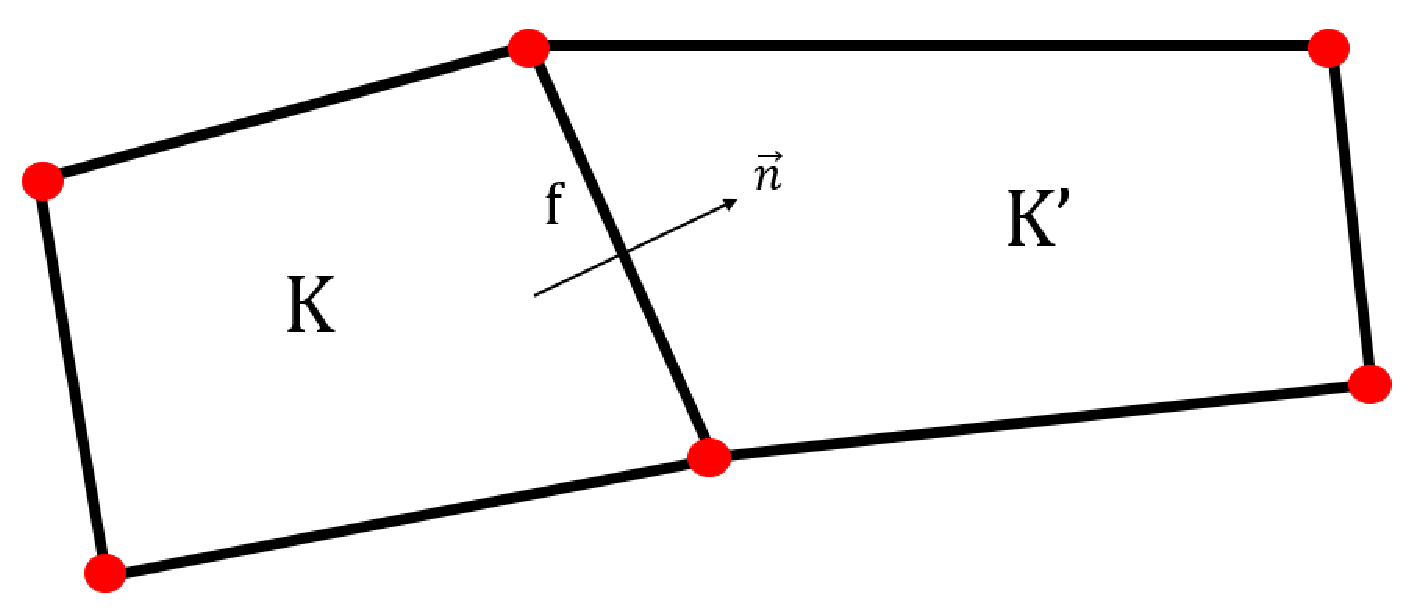
\includegraphics[width=0.7\textwidth]{figures/sec_Sn/two_cells_Rev1.eps}
\caption[Two cells of the spatial discretization]{Two cells of the spatial discretization with the connecting face, $f$, with normal direction, $\vec{n}$, oriented from cell $K$ to cell $K'$.}
\label{fig::Sn_two_ref_cells}
\end{figure}

Next, we left-multiply Eq. (\ref{eq::Sn_trans_eq_simple_no_energy_groups}) by an appropriate test function $b_m$, integrate over cell $K$, and apply Gauss' Divergence Theorem to the streaming term to obtain the Galerkin weighted-residual for cell $K$ for an angular direction $\vec{\Omega}_m$:

\begin{equation}
\label{eq::Sn_DGFEM_trans_eq_cellK}
\begin{aligned}
- \left( \vec{\Omega}_m \cdot  \vec{\nabla} b_m, \Psi_{m} \right)_{K} + \sum_{f=1}^{N_f^K} \Big< ( \vec{\Omega}_m \cdot \vec{n} ) \, b_m, \tilde{\Psi}_m  \Big>_{f}  + \Big(  \sigma_{t} b_m ,   \Psi_{m} \Big)_{K} \\
= \sum_{p=0}^{N_P} \sum_{n=-p}^{p} \frac{2p + 1}{4 \pi}  Y_{p,n} (  \vec{\Omega}_m ) \left[ \Big( \sigma_{s,p} \, b_m,  \Phi_{p,n,} \Big)_{K}  + \left(  b_m ,   Q_{p,n} \right)_{K} \right]
\end{aligned} .
\end{equation}

\noindent The cell boundary fluxes, $\tilde{\Psi}_m$, will depend on the cell boundary type and will be defined shortly. The cell boundary $\partial \mathcal{D}_K = \bigcup_{ f \in N_f^K} f$ is the closed set of the $N_f^K$ faces of the geometric cell. The inner products:

\begin{equation}
\label{eq::Sn_spatial_inner_products_cell}
 \Big( f, g \Big)_K \equiv \int_K f \, g \, d r
\end{equation} 

\noindent and

\begin{equation}
\label{eq::Sn_spatial_inner_products_face}
 \Big< f, g \Big>_f \equiv \int_f f \, g \, d s
\end{equation}

\noindent correspond to integrations over the cell and faces, respectively, where $dr \in \mathbb{R}^d$ is within the cell and $ds \in \mathbb{R}^{d-1}$ is along the cell boundary. We note that we will use this notation of the inner product for the remainder of the dissertation unless otherwise stated. We then separate the summation of the cell $K$ boundary integration terms into two different types: outflow boundaries ($\partial K^+ = \{  \vec{r} \in \partial K: \vec{n} (\vec{r}) \cdot \vec{\Omega}_m > 0 \}$) and inflow boundaries ($\partial K^- = \{  \vec{r} \in \partial K: \vec{n} (\vec{r}) \cdot \vec{\Omega}_m < 0 \}$). The inflow boundaries can further be separated into inflow from another cell: $\partial K^- \backslash \partial \mathcal{D} $; inflow from incident flux on the domain boundary: $\partial K^- \cap \partial \mathcal{D}^d $; and reflecting domain boundaries: $\partial K^- \cap \partial \mathcal{D}^r $. At this point, we note that the derivation can comprise an additional step by using Gauss' Divergence Theorem again on the streaming term. This is sometimes performed for radiation transport work so that mass matrix lumping can be performed, but we will not do so here. Therefore, with the cell boundary terminology as proposed, Eq. (\ref{eq::Sn_DGFEM_trans_eq_cellK}) can be written into the following form:

\begin{equation}
\label{eq::Sn_DGFEM_trans_eq_cellK_diff_faces}
\begin{aligned}
- \left( \vec{\Omega}_m \cdot  \vec{\nabla} b_m, \Psi_{m} \right)_{K}   + \Big(  \sigma_{t} b_m ,   \Psi_{m} \Big)_{K}  \\
+  \Big< ( \vec{\Omega}_m \cdot \vec{n} ) \, b_m, \tilde{\Psi}_m  \Big>_{\partial K^+}  + \Big< ( \vec{\Omega}_m \cdot \vec{n} ) \, b_m, \tilde{\Psi}_m  \Big>_{\partial K^- \backslash \partial \mathcal{D}} \\
  + \Big< ( \vec{\Omega}_m \cdot \vec{n} ) \, b_m, \tilde{\Psi}_m  \Big>_{\partial K^- \cap \partial \mathcal{D}^d}  + \Big< ( \vec{\Omega}_m \cdot \vec{n} ) \, b_m, \tilde{\Psi}_m  \Big>_{\partial K^- \cap \partial \mathcal{D}^r}  \\
= \sum_{p=0}^{N_P} \sum_{n=-p}^{p} \frac{2p + 1}{4 \pi}  Y_{p,n} (  \vec{\Omega}_m ) \left[ \Big( \sigma_{s,p} \, b_m,  \Phi_{p,n,} \Big)_{K}  + \left(  b_m ,   Q_{p,n} \right)_{K} \right]
\end{aligned} .
\end{equation}

We can now deal with the boundary fluxes, $\tilde{\Psi}_m$, by enforcing the ubiquitously-used {\em upwind scheme}. In simple nomenclature, the upwind scheme corresponds to using the angular flux values within the cell for outflow boundaries and angular flux values outside the cell for inflow boundaries. Mathematically, the upwind scheme can succinctly be written as the following for all boundary types,

\begin{equation}
\label{eq::Sn_upwind_cases}
\tilde{\Psi}_m (\vec{r}) = \begin{cases}
\Psi_m^{-} , & \partial K^+ \\
\Psi_m^{+}, & \partial K^- \backslash \partial \mathcal{D} \\
\Psi_m^{inc}, & \partial K^- \cap \partial \mathcal{D}^d \\
\Psi_{m'}^{-}, & \partial K^- \cap \partial \mathcal{D}^r
\end{cases} ,
\end{equation}

\noindent when the following trace is applied to the angular fluxes :

\begin{equation}
\label{eq::Sn_ang_flux_trace}
\Psi_m^{\pm} (\vec{r}) \equiv \lim_{s \rightarrow 0^{\pm}} \Psi_m \Big( \vec{r} + s (\vec{\Omega}_m \cdot \vec{n}) \vec{n} \Big) .
\end{equation}

\noindent This trace has the notation, with $\vec{n}$ pointing outwards from cell $K$, of $\Psi_m^-$ corresponding to fluxes within the cell and $\Psi_m^+$ corresponding to fluxes out of the cell. Now, using the upwind scheme as previously defined, we can write our complete set of DGFEM equations for cell $K$ as

\begin{equation}
\label{eq::Sn_DGFEM_trans_eq_cellK_complete}
\begin{aligned}
-  \Big( \vec{\Omega}_m \cdot  & \vec{\nabla} b_m, \Psi_{m} \Big)_{K}   + \Big(  \sigma_{t} b_m ,   \Psi_{m} \Big)_{K} +  \Big< ( \vec{\Omega}_m \cdot \vec{n} ) \, b_m, {\Psi}_m^{-}  \Big>_{\partial K^+}  \\
  + & \Big< ( \vec{\Omega}_m \cdot \vec{n} ) \, b_m, {\Psi}_m^{+}  \Big>_{\partial K^- \backslash \partial \mathcal{D}}  + \Big< ( \vec{\Omega}_m \cdot \vec{n} ) \, b_m, {\Psi}^{-}_{m'}  \Big>_{\partial K^- \cap \partial \mathcal{D}^r}  \\
= & \sum_{p=0}^{N_P} \sum_{n=-p}^{p} \frac{2p + 1}{4 \pi}  Y_{p,n} (  \vec{\Omega}_m ) \left[ \Big( \sigma_{s,p} \, b_m,  \Phi_{p,n,} \Big)_{K}  + \left(  b_m ,   Q_{p,n} \right)_{K} \right] \\
+ & \Big< ( \vec{\Omega}_m \cdot \vec{n} ) \, b_m, {\Psi}_m^{inc}  \Big>_{\partial K^- \cap \partial \mathcal{D}^d}
\end{aligned} .
\end{equation} 

\noindent We note that fluxes without the trace superscript are all within the cell. By completely defining our mathematical formulation for an arbitrary spatial cell, it is easy to see that the full set of equations to define our discretized solution space for a single angle and energy group comprises of a simple double integration loop. The full set of equations can be formed by looping over all spatial cells, $\mathcal{D} = \bigcup_{K \in \mathbb{T}_h} K$, while further looping over all faces within each cell, $\partial \mathcal{D}_K = \bigcup_{ f \in N_f^K} f$. 

%%%%%%%%%%%%%%%%%%%%%%%%%%%%%%%%%%%%%%%%%%%%%%%%%%%
%%%   SubSection - Convergence
\subsection{Convergence Rates of the DGFEM $S_N$ Equation}
\label{sec::Sn_Spatial_Convergence}

This double integration loop allows us to write the variational form for the one-group $S_N$ equation. We do this by taking Eq. (\ref{eq::Sn_DGFEM_trans_eq_cellK_complete}), performing another integration-by-parts on the streaming term, mulitplying by the angular weight, $w_m$, and summing over all elements and all angular directions. 




%%%%%%%%%%%%%%%%%%%%%%%%%%%%%%%%%%%%%%%%%%%%%%%%%%%
%%%   SubSection - Elementary
\subsection{Elementary Matrices on an Arbitrary Spatial Cell}
\label{sec::Sn_Spatial_Matrices}

%%%%%%%%%%%%%%%%%%%%%%%%%%%%%%%%%%%%%%%%%%%%%%%%%%%
%%%   SubSection - Mass
\subsubsection{Elementary Mass Matrices}
\label{sec::Sn_Spatial_Matrices_Mass}

In the spatially discretized equations presented in Section \ref{sec::Sn_Spatial}, there are several reaction terms that appear with the form: $\Big( \sigma  b_m , \Psi_m  \Big)_K$ for a given angular direction, $m$, and for a spatial cell, $K$. In FEM analysis these reaction terms are ubiquitously referred to as the mass matrix terms \cite{zeinkiewicz2005finite,akin1982application}. For cell $K$, we define the elementary mass matrix, ${\bf M}$ as

\begin{equation}
\label{eq::Sn_mass_matrix_analytical}
{\bf M}_K =    \int_K {\bf b}_K \, {\bf b}_K^T \, d r ,
\end{equation}

\noindent where ${\bf b}_K$ corresponds to the set of $N_K$ basis functions that have non-zero measure in cell $K$. Depending on the FEM basis functions utilized, the integrals in Eq. (\ref{eq::Sn_mass_matrix_analytical}) can be directly integrated analytically. However, if in general, the basis functions cannot be analytically integrated on an arbitrary set of cell shapes, then a numerical integration scheme becomes necessary. If we define a quadrature set, $\left\{  \vec{x}_q , w_q^{K}  \right\}_{q=1}^{N_q}$, for cell $K$, consisting of $N_q$ points, $\vec{x}_q$, and weights, $w_q^K$, then we can numerically calculate the mass matrix by the following

\begin{equation}
\label{eq::Sn_mass_matrix_numerical}
{\bf M}_K =    \sum_{q = 1}^{N_q} w_{q}^K {\bf b}_K (\vec{x}_q) \, {\bf b}_K^T (\vec{x}_q)  .
\end{equation}

\noindent In this case, it is necessary that the sum of the weights of this quadrature set exactly equal the geometric measure of cell $K$. This means that $\sum_{q = 1}^{N_q} w_{q}^K$ is equal to the cell width in 1 dimension, the cell area in 2 dimensions, and the cell volume in 3 dimensions.

Since ${\bf b}_K$ consists of a column vector for the basis functions and ${\bf b}_K^{T}$ consists of a row vector, then their multiplication will obviously yield a full $(N_K \, \text{x} \, N_K)$ matrix. This matrix is written for completeness of this discussion on the mass matrix:

\begin{equation}
\label{eq::Sn_mass_matrix_array}
{\bf M}_K =   \left[
\begin{array} {ccccc}
	\int_K b_1 \, b_1  & \ldots & \int_K b_1 \, b_j  & \ldots & \int_K b_1 \, b_{N_K} \\
	\vdots  &  & \vdots  &  & \vdots \\
	\int_K b_i \, b_1  & \ldots & \int_K b_i \, b_j  & \ldots & \int_K b_i \, b_{N_K} \\
	\vdots  &  & \vdots  &  & \vdots \\
	\int_K b_{N_K} \, b_1  & \ldots & \int_K b_{N_K} \, b_j  & \ldots & \int_K b_{N_K} \, b_{N_K} \\
\end{array}
\right] ,
\end{equation}

\noindent where an individual matrix entry is of the form:

\begin{equation}
\label{eq::Sn_mass_matrix_entry}
M_{i,j,K} =  \int_K b_i \, b_j .
\end{equation}

%%%%%%%%%%%%%%%%%%%%%%%%%%%%%%%%%%%%%%%%%%%%%%%%%%%
%%%   SubSection - Streaming
\subsubsection{Elementary Streaming Matrices}
\label{sec::Sn_Spatial_Matrices_Streaming}

Next, we will consider the streaming term that has the form: $ \Big( \vec{\Omega}_m \cdot \vec{\nabla}  b_m , \Psi_m  \Big)_K$ for a given angular direction, $m$, and for a spatial cell, $K$. $\vec{\nabla} $ is the gradient operator in physical space. It has the form of $\vec{\nabla} = \left[ \frac{d}{dx} \right]$ in 1 dimension, the form of $\vec{\nabla} = \left[ \frac{\partial}{\partial x} , \frac{\partial}{\partial y} \right]$ in 2 dimensions, and the form of $\vec{\nabla} = \left[ \frac{\partial}{\partial x} , \frac{\partial}{\partial y} , \frac{\partial}{\partial z} \right]$ in 3 dimensions. Since for every cell, the streaming term is applied for all $M$ angles in the angular discretization, we define the analytical elementary streaming matrix:

\begin{equation}
\label{eq::Sn_streaming_matrix_analytical}
\vec{{\bf G}}_K =    \int_K \vec{\nabla} {\bf b}_K \, {\bf b}_K^T \, d r ,
\end{equation}

\noindent which has dimensionality $(N_K \text{x} N_K \text{x} d)$. We choose to store the elementary streaming matrix in this form and not store $M$ separate $(N_K \text{x} N_K)$ local matrices corresponding to the application of the dot product ($ \vec{\Omega}_m  \cdot \int_K  \vec{\nabla} {\bf b}_K \, {\bf b}_K^T \, d r$). Instead we simply evaluate the dot product with the appropriate angular direction whenever necessary. This has great benefit when trying to run large transport problems when memory becomes a premium and processor operations are not our limiting bottleneck. 

Just like the elementary mass matrix, we can use the same spatial quadrature set, $\left\{  \vec{x}_q , w_q^{K}  \right\}_{q=1}^{N_q}$, for cell $K$ to numerically calculate the streaming matrix:

\begin{equation}
\label{eq::Sn_streaming_matrix_numerical}
\vec{{\bf G}}_K =    \sum_{q = 1}^{N_q} w_{q}^K \vec{\nabla} {\bf b}_K (\vec{x}_q) \, {\bf b}_K^T (\vec{x}_q) .
\end{equation}

\noindent In this case, this local cell-wise streaming matrix has the full matrix form:

\begin{equation}
\label{eq::Sn_streaming_matrix_array}
\vec{{\bf G}}_K =   \left[
\begin{array} {ccccc}
	\int_K \vec{\nabla}b_1 \, b_1  & \ldots & \int_K \vec{\nabla}b_1 \, b_j  & \ldots & \int_K \vec{\nabla}b_1 \, b_{N_K} \\
	\vdots  &  & \vdots  &  & \vdots \\
	\int_K \vec{\nabla} b_i \, b_1  & \ldots & \int_K \vec{\nabla}b_i \, b_j  & \ldots & \int_K \vec{\nabla}b_i \, b_{N_K} \\
	\vdots  &  & \vdots  &  & \vdots \\
	\int_K \vec{\nabla} b_{N_K} \, b_1  & \ldots & \int_K \vec{\nabla} b_{N_K} \, b_j  & \ldots & \int_K \vec{\nabla} b_{N_K} \, b_{N_K} \\
\end{array}
\right] ,
\end{equation}

\noindent where an individual matrix entry is of the form:

\begin{equation}
\label{eq::Sn_streaming_matrix_entry}
\vec{G}_{i,j,K} =  \int_K \vec{\nabla}b_i \, b_j .
\end{equation}

%%%%%%%%%%%%%%%%%%%%%%%%%%%%%%%%%%%%%%%%%%%%%%%%%%%
%%%   SubSection - Surface
\subsubsection{Elementary Surface Matrices}
\label{sec::Sn_Spatial_Matrices_Surface}

Finally, the last terms to consider of the discretized transport equation are those found on the faces of the cell boundary: $  \vec{\Omega}_m \cdot  \Big<  \vec{n} \, b_m, \Psi_m  \Big>_{\partial K}$. These terms are analagous to the cell mass matrix but are computed on the cell boundary with dimensionality $(d-1)$. Analyzing a single face, $f$, in cell $K$, the analytical surface matrix is of the form,

\begin{equation}
\label{eq::Sn_surface_matrix_analytical}
\vec{{\bf F}}_{f,K}  =    \int_f \vec{n} (\vec{r}) \, {\bf b}_K \, {\bf b}_K^T \, d s ,
\end{equation}

\noindent where we allow the outward surface normal, $\vec{n}$, to vary along the cell face. For 1D problems as well as 2D problems with colinear cell faces (no curvature), the outward normals would be constant along the entire face. However, there are many cases where 3D mesh cells would not have coplanar vertices along a face. Then, the outward normal would not be constant along the face and would need to be taken into account during integration procedures. A simple example of non-coplanar face vertices would be an orthogonal hexahedral cell that has its vertices undergo a randomized displacement.

With the analytical form of the surface matrices defined in Eq. (\ref{eq::Sn_surface_matrix_analytical}), we can see that they have dimensionality, $(N_K \text{x} N_K \text{x} d)$. This is the same dimensionality as the cell streaming term. However, it is possible to reduce the dimensionality of the surface matrices if it is desired to reduce the memory footprint. There are some basis sets where all but $N_b^{f,K}$ basis functions are zero along face $f$. If we also restrict the mesh cell faces of our transport problems to have colinear (in 2D) or coplanar (in 3D) vertices so that the outward normal is constant along a face $f$, then we can define the surface matrix as $\int_f {\bf b}_K \, {\bf b}_K^T \, d s$. For these basis sets with $N_b^{f,K}$ non-zero face values on colinear/coplanar face $f$, the surface matrix has reduced dimensionality of $(N_b^{f,K} \text{x} N_b^{f,K})$.

Just like the cell mass and streaming matrices, it is possible that the basis functions cannot be integrated analytically. Analogous to the cell-wise quadrature, we can define a quadrature set for  face face $f$: $\left\{  \vec{x}_q , w_q^{f}  \right\}_{q=1}^{N_q^f}$. This quadrature set is not specific for just one of the cells that face $f$ separates. If the quadrature set can exactly integrate the basis functions of both cells $K$ and $K'$ (as defined by Figure \ref{fig::Sn_two_ref_cells}), then only 1 quadrature set needs to be defined for both cells. Using this quadrature set, we can numerically calculate the surface matrix for face $f$ along cell $K$:

\begin{equation}
\label{eq::Sn_surface_matrix_numerical}
\vec{{\bf F}}_{f,K} =    \sum_{q = 1}^{N_q^f} w_{q}^f \vec{n} (\vec{x}_q) \, {\bf b}_K (\vec{x}_q) \, {\bf b}_K^T (\vec{x}_q) .
\end{equation}

\noindent Similar to the cell-wise spatial quadrature sets, the sum of the weights of these face-wise quadrature sets need to exactly equal the geometric measure of face $f$. This means that $\sum_{q = 1}^{N_q^f}$ is equal to 1.0 in 1 dimension, the length of the face edge in 2 dimensions and the face area in 3 dimensions. 

Using the same notation as the cell-wise mass and streaming matrices, the local face-wise surface matrix for face $f$ has the full matrix form,

\begin{equation}
\label{eq::Sn_surface_matrix_array}
\vec{{\bf F}}^{f,K} =   \left[
\begin{array} {ccccc}
	\int_f \vec{n} \, b_1 \, b_1  & \ldots & \int_f \vec{n} \, b_1 \, b_j  & \ldots & \int_f \vec{n} \, b_1 \, b_{N_K} \\
	\vdots  &  & \vdots  &  & \vdots \\
	\int_f \vec{n} \,  b_i \, b_1  & \ldots & \int_f \vec{n} \, b_i \, b_j  & \ldots & \int_f \vec{n} \, b_i \, b_{N_K} \\
	\vdots  &  & \vdots  &  & \vdots \\
	\int_f \vec{n} \,  b_{N_K} \, b_1  & \ldots & \int_f \vec{n} \,  b_{N_K} \, b_j  & \ldots & \int_f \vec{n} \,  b_{N_K} \, b_{N_K} \\
\end{array}
\right] ,
\end{equation}

\noindent where an individual matrix entry is of the form:

\begin{equation}
\label{eq::Sn_streaming_matrix_entry}
\vec{{ F}}_{i,j,f,K} =  \int_f \vec{n} \, b_i \, b_j .
\end{equation}

%%%%%%%%%%%%%%%%%%%%%%%%%%%%%%%%%%%%%%%%%%%%%%%%%%%
%%%   Section - Solution Procedures
\section{Solution Procedures}
\label{sec::Sn_Solution}

To this point, we have properly described the procedures to discretize the transport problem in energy, angle, and space. Combining the results of Sections \ref{sec::Sn_MG}, \ref{sec::Sn_Angle}, and \ref{sec::Sn_Spatial}, we write the fully-discretized DGFEM multigroup $S_N$ equations for an element $K$, where the test function $b_{m,g}$ for a single direction and energy group is now used:

\begin{equation}
\label{eq::Sn_DGFEM_trans_eq_cellK_bmg_complete}
\begin{aligned}
-  \Big( \vec{\Omega}_m \cdot  & \vec{\nabla} b_{m,g}, \Psi_{m,g} \Big)_{K}   + \Big(  \sigma_{t,g} b_{m,g} ,   \Psi_{m,g} \Big)_{K} +  \Big< ( \vec{\Omega}_m \cdot \vec{n} ) \, b_{m,g}, {\Psi}_{m,g}^{-}  \Big>_{\partial K^+}  \\
  + & \Big< ( \vec{\Omega}_m \cdot \vec{n} ) \, b_{m,g}, {\Psi}_{m,g}^{+}  \Big>_{\partial K^- \backslash \partial \mathcal{D}}  + \Big< ( \vec{\Omega}_m \cdot \vec{n} ) \, b_{m,g}, {\Psi}^{-}_{m',g}  \Big>_{\partial K^- \cap \partial \mathcal{D}^r}  \\
= & \sum\displaylimits_{g'=1}^G \sum_{p=0}^{N_P} \frac{2p + 1}{4 \pi} \sum_{n=-p}^{p}   Y_{p,n} (  \vec{\Omega}_m )  \Big( \sigma_{s,p}^{g' \rightarrow g} \, b_{m,g},  \Phi_{p,n,g'} \Big)_{K}  \\
+ & \left(  b_{m,g} ,   Q_{m,g} \right)_{K} + \Big< ( \vec{\Omega}_m \cdot \vec{n} ) \, b_{m,g}, {\Psi}_{m,g}^{inc}  \Big>_{\partial K^- \cap \partial \mathcal{D}^d}
\end{aligned} .
\end{equation} 

\noindent All of the notations used in Eq. (\ref{eq::Sn_DGFEM_trans_eq_cellK_bmg_complete}) remain unchanged from Section \ref{sec::Sn_Spatial}.

We now spend the remainder of this chapter discussing various methodologies to efficiently solve the tightly-coupled system of equations composing our transport problem. Section \ref{sec::Sn_Solution_Iterative} details the iterative procedures used to solve the transport problem in energy and angle, and Section \ref{sec::Sn_Solution_Spatial} then describes how we solve the spatial portion of the problem for a single energy/angle iteration.

%%%%%%%%%%%%%%%%%%%%%%%%%%%%%%%%%%%%%%%%%%%%%%%%%%%
%%%   SubSection - Iterative Procedures
\subsection{Angle and Energy Iteration Procedures}
\label{sec::Sn_Solution_Iterative}

The fully discretized transport equation has an angular flux solution, ${\bf \Psi}$, with dimensionality of $(G \text{x} M \text{x} N_{dof})$. The angular flux moments, ${\bf \Phi}$, have dimensionality of $(G \text{x} N_{mom} \text{x} N_{dof})$. Depending on the necessary fidelity of the problem, the full phase-space of the solution can become extremely large to solve. We can have {\em billions} of total unkowns to solve for if we simply have $N_{dof} \approx O(10^6)$, $M \approx O(10^2)$, and $G \approx O(10^1)$. These orders of number of unknowns in space, angle, and energy are of reasonable size for 3D transport problems.

In theory, if we had the computer memory, we could construct a left-hand-side matrix of dimensionality $(G \text{x} M \text{x} N_{dof})$x$(G \text{x} M \text{x} N_{dof})$ with a corresponding right-hand-side vector of dimensionality $(G \text{x} M \text{x} N_{dof})$x1, we could then directly solve for the full phase-space angular flux solution at once. However, because the dimensional space of the unknowns can rapidly grow and become to large for hardware memory, transport problems have traditionally been solved iteratively. We now detail the procedures that we will employ to iteratively obtain the phase-space solution in energy and angle.

\begin{figure}
\centering
	\begin{subfigure}[b]{0.58\textwidth}
		\centering
		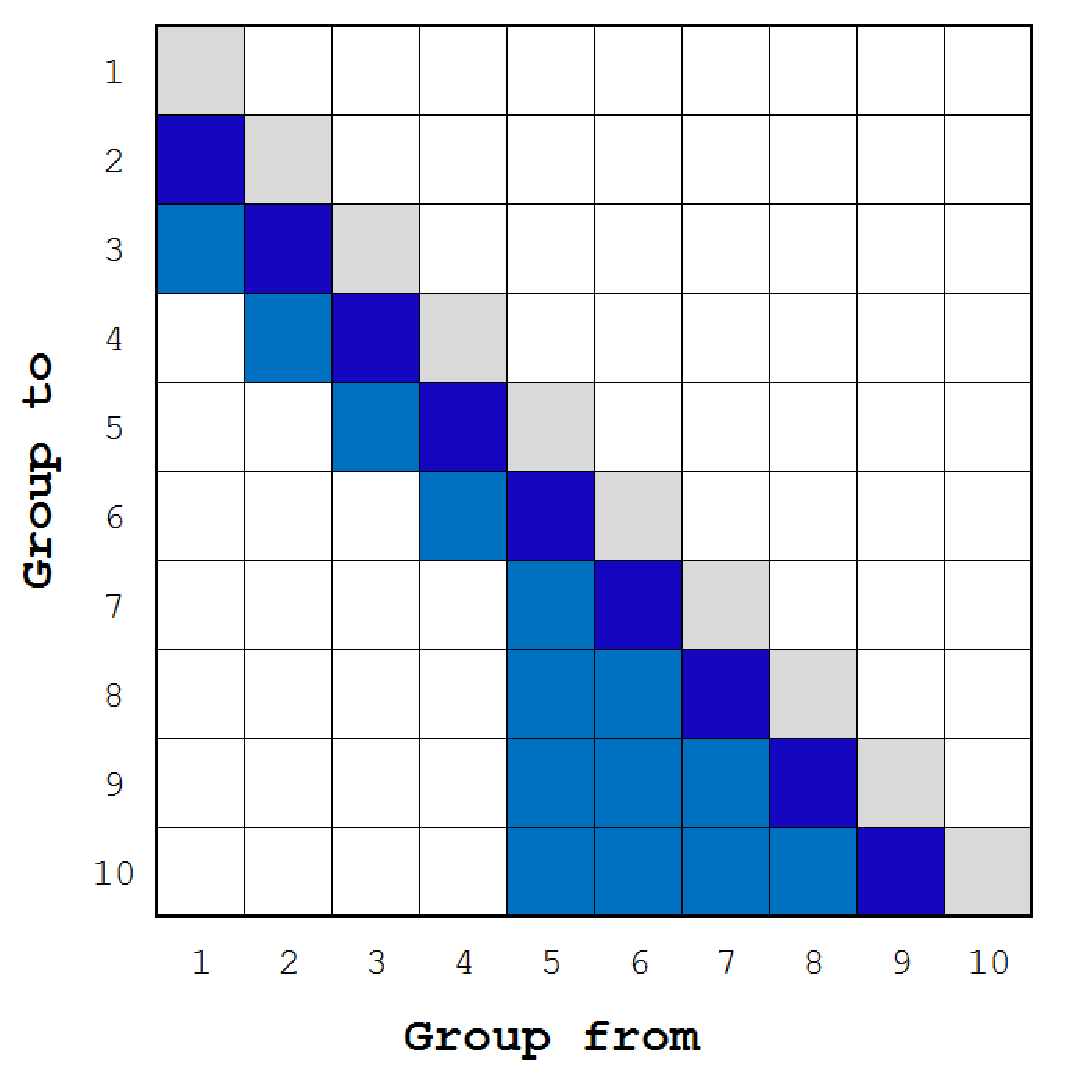
\includegraphics[width=\textwidth]{figures/sec_Sn/scattering_matrix_NO_upscattering.eps}
		\vspace{4mm}
	\end{subfigure}
	\hfill
	\begin{subfigure}[b]{0.58\textwidth}
		\centering
		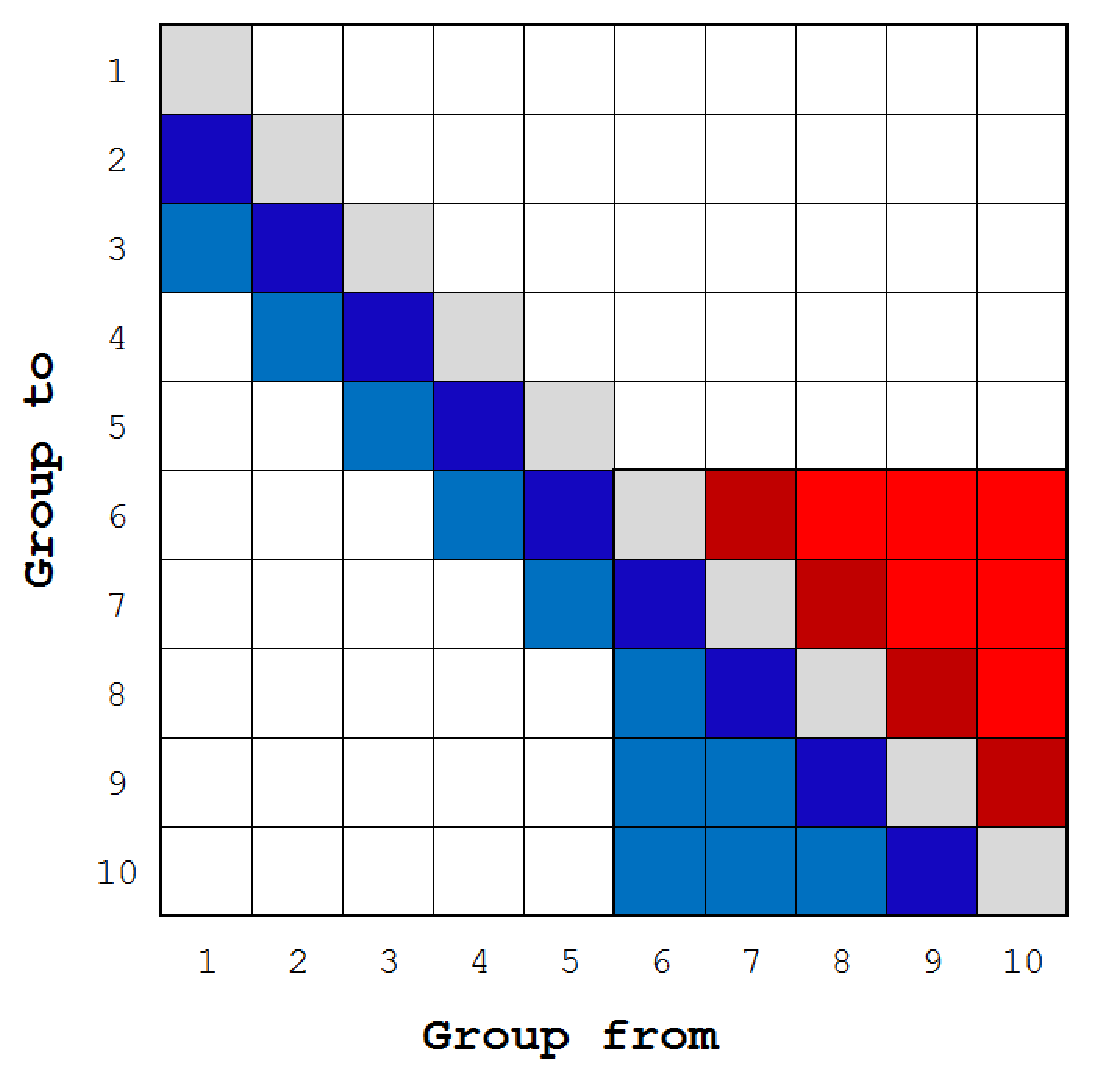
\includegraphics[width=\textwidth]{figures/sec_Sn/scattering_matrix_w_upscattering.eps}
	\end{subfigure}
\caption[Scattering matrices with and without upscattering]{Scattering matrices (top) without and (bottom) with upscattering. The gray corresponds to within-group scattering; the blue corresponds to down-scattering in energy; and the red corresponds to up-scattering in energy.}
\label{fig::Sn_Solution_Iterative_scattmatrix}
\end{figure}

\begin{equation}
\label{eq::Sn_full_sol_ops}
\begin{aligned}
{\bf L} {\bf \Psi} - {\bf M} {\bf \Sigma} {\bf \Phi}  =    {\bf Q} \\
{\bf \Phi} =  {\bf D} {\bf \Psi}
\end{aligned}
\end{equation}

\noindent where ${\bf L}$ is the fully-discretized loss operator which consists of total interaction and streaming terms, ${\bf M}$ is the moment-to-discrete operator of the angular discretization, ${\bf D}$ is the discrete-to-moment operator of the angular discretization, ${\bf \Sigma}$ is the scattering operator of the multigroup and angular discretizations, and ${\bf Q}$ is the full phase-space distributed source. In this case the source contains contributions from boundary and domain sources, fission sources, and scattering sources from outside the group set into the group set of interest.



\begin{equation}
\label{eq::Sn_full_sol_moments_only}
\left( {\bf I} -{\bf T} \right) {\bf \Phi} =  {\bf D} {\bf L}^{-1}  {\bf Q} 
\end{equation}

\noindent where we define,

\begin{equation}
\label{eq::Sn_trans_op_T}
{\bf T} \equiv {\bf D} {\bf L}^{-1}{\bf M} {\bf \Sigma} ,
\end{equation}

\noindent for further brevity.



%%%%%%%%%%%%%%%%%%%%%%%%%%%%%%%%%%%%%%%%%%%%%%%%%%%
%%%   SubSubSection - Source Iteration
\subsubsection{Source Iteration}
\label{sec::Sn_Solution_Iterative_SI}

One simple method to invert $({\bf I} - {\bf T})$ of Eq. (\ref{eq::Sn_full_sol_moments_only}) is the {\em source iteration} technique, also known as {\em richardson iteration}.

\begin{equation}
\label{eq::Sn_si_iter}
\begin{aligned}
 {\bf \Psi}^{(\ell+1)} = {\bf L}^{-1}  {\bf M} {\bf \Sigma} {\bf \Phi}^{(\ell)} + {\bf L}^{-1}  {\bf Q} \\
{\bf \Phi}^{(\ell+1)} =  {\bf D} {\bf \Psi}^{(\ell+1)}
\end{aligned}
\end{equation}

%%%%%%%%%%%%%%%%%%%%%%%%%%%%%%%%%%%%%%%%%%%%%%%%%%%
%%%   SubSubSection - Source Iteration
\subsubsection{Krylov Subspace Methods - GMRES}
\label{sec::Sn_Solution_Iterative_GMRES}

%%%%%%%%%%%%%%%%%%%%%%%%%%%%%%%%%%%%%%%%%%%%%%%%%%%
%%%   SubSection - Spatial Solution Procedures
\subsection{Spatial Solution Procedures}
\label{sec::Sn_Solution_Spatial}

Section \ref{sec::Sn_Solution_Iterative} presented the methodology that we will employ to iteratively converge our transport solutions in energy and angle (flux moments). Both richardson iteration and GMRES were presented as methods that can invert the $({\bf I} - {\bf T})$ operator. In both of these iterative methods, the common operation of interest is the inversion of the loss operator (${\bf L}$). There are different techniques that could be used to perform this operation, including serveral matrix-dependent and matrix-free methodologies. 

For this work, the loss operator inversion on some unstructured mesh, $\mathbb{T}_h$, will be performed by use of the full-domain transport sweep as outlined next in Section \ref{sec::Sn_Solution_Spatial_Sweeping}. We will generate our 2D and 3D polytope meshes by two different methods: 1) Voronoi mesh generation in Section \ref{sec::Sn_Solution_Spatial_Voronoi} and 2) adaptive mesh refinement in Section \ref{sec::Sn_Solution_Spatial_AMR}.

%%%%%%%%%%%%%%%%%%%%%%%%%%%%%%%%%%%%%%%%%%%%%%%%%%%
%%%   SubSubSection - Transport Sweeping
\subsubsection{Transport Sweeping}
\label{sec::Sn_Solution_Spatial_Sweeping}

The full-domain transport sweep is a beneficial matrix-free scheme because of the following:

\begin{itemize}
\item The number of sweep iterations does not grow with increasing problem size or processor counts. This is in contrast with partial-domain sweeping like {\em parallel block jacobi} (PBJ) \cite{zerr2011solution}.
\item Does not require the formation of $M$ separate matrices for each of the angular directions. 
\item 
\end{itemize}

\begin{figure}
\centering
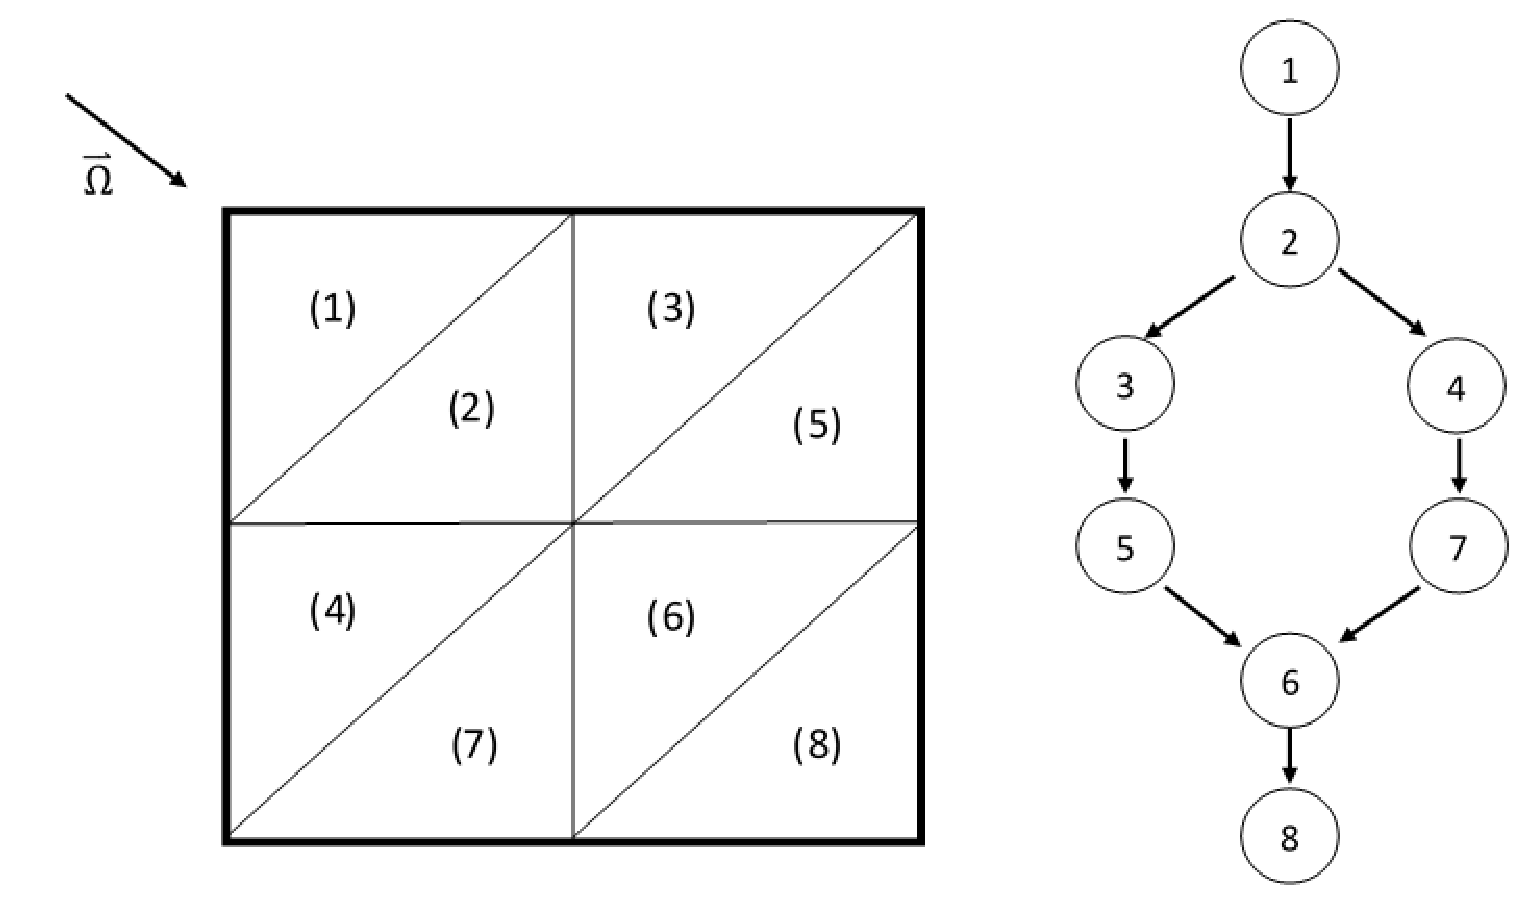
\includegraphics[width=0.75\textwidth]{figures/sec_Sn/triangle_graph_nocycle.eps}
\caption[blah]{blah.}
\label{fig::Sn_Solution_Spatial_Sweeping_sweepNOcycle}
\end{figure}

\begin{figure}
\centering
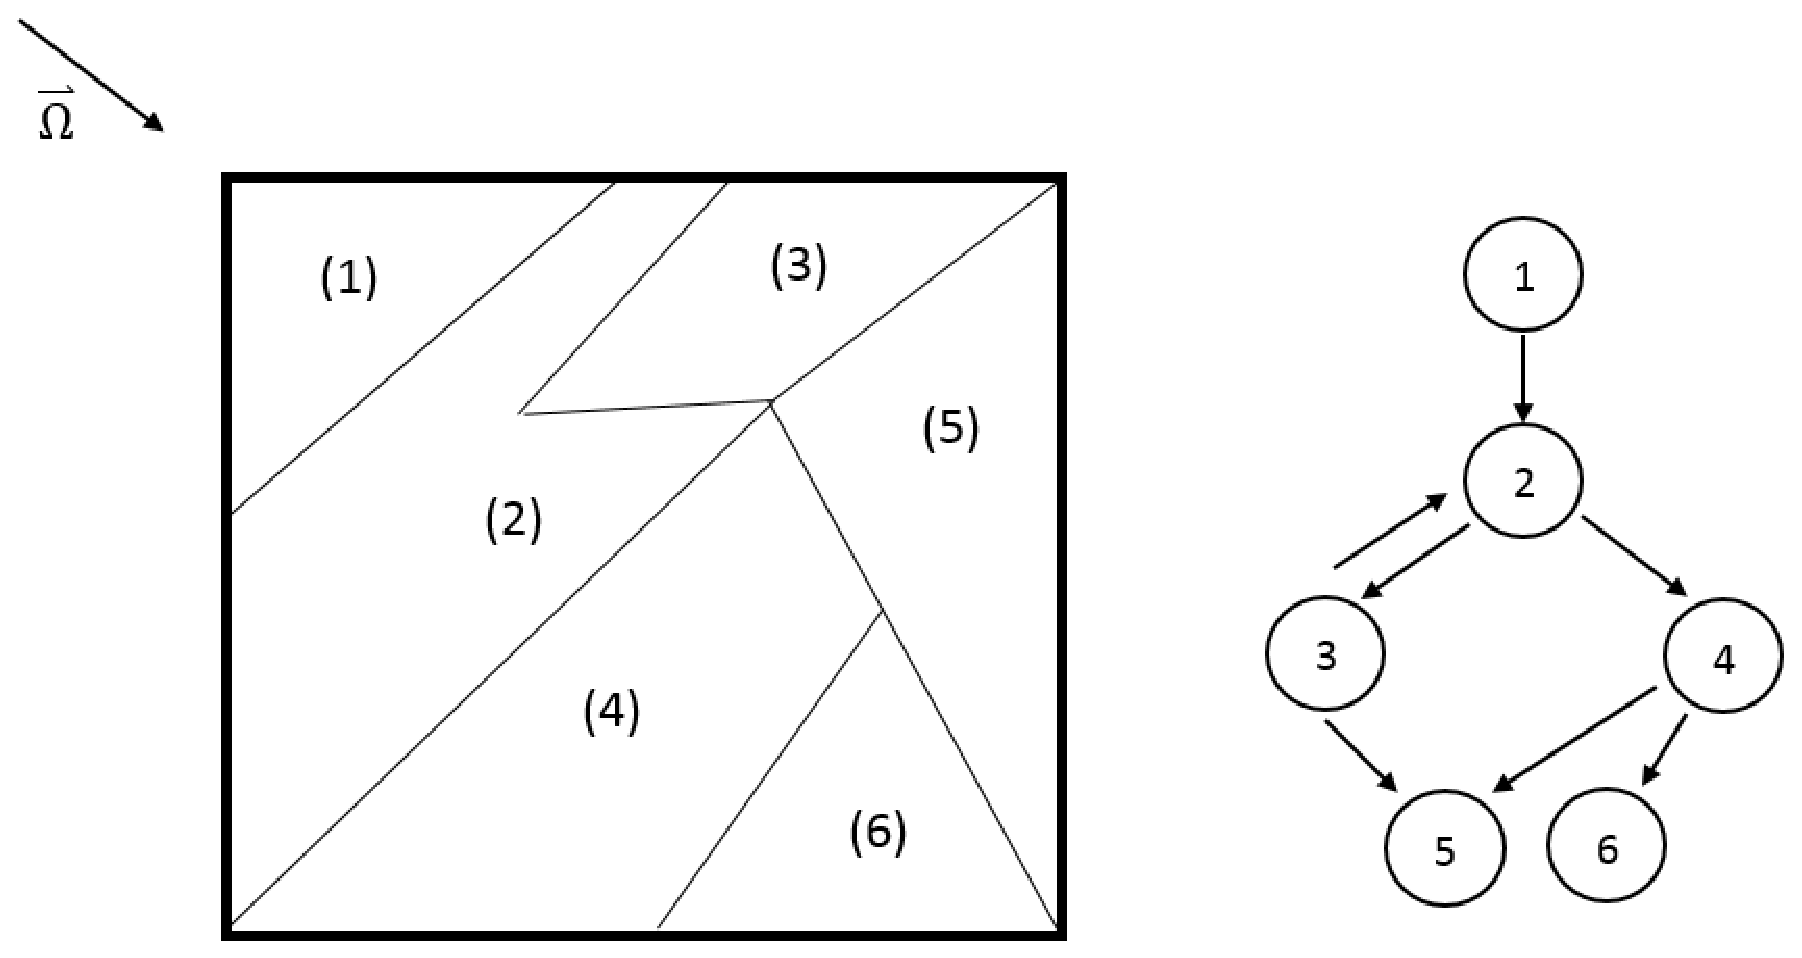
\includegraphics[width=0.75\textwidth]{figures/sec_Sn/graph_with_cycling.eps}
\caption[blah]{blah.}
\label{fig::Sn_Solution_Spatial_Sweeping_sweepWcycle}
\end{figure}

%%%%%%%%%%%%%%%%%%%%%%%%%%%%%%%%%%%%%%%%%%%%%%%%%%%
%%%   SubSubSection - Voronoi
\subsubsection{Polytope Grids Formed from Voronoi Mesh Generation}
\label{sec::Sn_Solution_Spatial_Voronoi}



%%%%%%%%%%%%%%%%%%%%%%%%%%%%%%%%%%%%%%%%%%%%%%%%%%%
%%%   SubSubSection - AMR
\subsubsection{Spatial Adaptive Mesh Refinement}
\label{sec::Sn_Solution_Spatial_AMR}



\begin{equation}
\label{eq::Sn_AMR_jump_err_est}
\eta_K^r = \int\displaylimits_{\partial K} [\![ \Phi^r ]\!]^2 d \, s = \int\displaylimits_{\partial K} \left(  \sum_m w_m [\![ \Psi_m^r ]\!]  \right)^2
\end{equation}

\noindent where $[\![ \cdot ]\!]$ is the jump operator along a face defined as,

\begin{equation}
\label{eq::Sn_AMR_jump_def}
[\![ \Phi (\vec{r}) ]\!] = \Phi^+ (\vec{r}) - \Phi^- (\vec{r}),
\end{equation}

\noindent and the terms,$\Phi^+ (\vec{r})$ and $\Phi^- (\vec{r})$, are subject to the trace:

\begin{equation}
\label{eq::Sn_AMR_jump_trace}
\Phi^{\pm} (\vec{r})  = \lim\displaylimits_{s \rightarrow 0^{\pm}} \Phi (\vec{r} + s \vec{n}).
\end{equation}

\noindent In this case, the outward normal, $\vec{n}$, is determined with respect to the element $K$ along its boundary, $\partial K$. With this trace, $\Phi^- (\vec{r})$ always corresponds to the solution within cell $K$. Investigating face $f$ of cell $K$, the across-face solution, $\Phi^+ (\vec{r})$, is dependent on the boundary type of face $f$. The across-face solutions can be succinctly writen:

\begin{equation}
\label{eq::Sn_AMR_across_face_vals}
\Phi^+ (\vec{r}) = 
\begin{cases}
\lim\displaylimits_{s \rightarrow 0^{+}} \Phi (\vec{r} + s \vec{n}) & \vec{r} \notin \partial \mathcal{D} \\
\sum\displaylimits_{\vec{\Omega}_m \cdot \vec{n} > 0}  \Psi_m^- (\vec{r}) + \sum\displaylimits_{\vec{\Omega}_m \cdot \vec{n} < 0} \Psi_{m}^{inc} (\vec{r}) & \vec{r} \in \partial \mathcal{D}^d \\
\Phi^- (\vec{r}) & \vec{r} \in \partial \mathcal{D}^r
\end{cases}.
\end{equation}

\noindent From Eq. (\ref{eq::Sn_AMR_across_face_vals}), the across-face solutions for interior faces, incident boundaries and reflecting boundaries have different meanings. For an interior face $f$ ($\vec{r} \notin \partial \mathcal{D}$), the across-face solution comes from the cell $K'$ (as defined by Figure \ref{fig::Sn_two_ref_cells}). For incident boundaries ($\vec{r} \in \partial \mathcal{D}^d$), the across-face solution is a combination of integrals of the outgoing ($\Psi_m^-$) and incident boundary fluxes ($\Psi_m^{inc}$). Finally, for reflecting boundaries ($\vec{r} \in \partial \mathcal{D}^r$), the across-face solutions are simply the within-cell solutions. Therefore, the solution jump is exactly zero for all reflecting boundaries and yields no contribution to the error estimate.

\begin{equation}
\label{eq::Sn_AMR_err_crit}
\eta_K^r \geq \alpha \max\displaylimits_{K' \in \mathbb{T}_h^r} \left(  \eta_{K'}^{r} \right)
\end{equation}

\noindent where $\alpha$ is a user-defined value $(0,1)$. This refinement criterion has a simple meaning. If, for example, $\alpha = 0.2$, then a cell will be refined if its error estimate is greater than 20\% of the cell with the largest error estimate. This does not necessarily mean that 80\% of the mesh cells will be refined at level $r$. Instead, the criterion simply states that any cell above a particular threshold will be refined. This means that it is theoretically possible for the extreme cases of 1 or all cells being refined at a particular refinement cycle.


%%%%%%%%%%%%%%%%%%%%%%%%%%%%%%%%%%%%%%%%%%%%%%%%%%%
%%%   Section - Conclusions
\section{Conclusions}
\label{sec::Sn_Conclusions}

In this chapter, we have presented the tightly-coupled system of equations that comprise the DGFEM $S_N$ transport equation. We began with the fully-continuous transport equation presented in Section \ref{sec::Sn_neut} and then discretized it in energy, angle and space in Sections \ref{sec::Sn_MG}, \ref{sec::Sn_Angle}, and \ref{sec::Sn_Spatial}, respectively. Appropriate boundary conditions were presented in Section \ref{sec::Sn_BC}. For this work, we will only utilize incoming-incident and reflecting boundary conditions and not use any further albedo terms. We finished this chapter in Section \ref{sec::Sn_Solution} by describing the procedures that will be utilized to solve our system of equations.


%%%%%%%%%%%%%%%%%%%%%%%%%%%%%%%%%%%%%%%%%%%%%%%%%%%%
%
%  New template code for TAMU Theses and Dissertations starting Fall 2012.  
%  For more info about this template or the 
%  TAMU LaTeX User's Group, see http://www.howdy.me/.
%
%  Author: Wendy Lynn Turner 
%	 Version 1.0 
%  Last updated 8/5/2012
%
%%%%%%%%%%%%%%%%%%%%%%%%%%%%%%%%%%%%%%%%%%%%%%%%%%%
%%%                           SECTION V
%%%%%%%%%%%%%%%%%%%%%%%%%%%%%%%%%%%%%%%%%%%%%%%%%%%
\chapter{\uppercase {FEM Basis Functions for Unstructured Polytopes}}
\label{sec::BF}



In Section \ref{sec::Sn_Spatial}, we detailed the spatial discretization of the transport equation. We then proceeded to give the functional forms for the various elementary matrices needed to form the full set of spatially-discretized PDEs. These included the mass, streaming, and surface matrices where the integrations on the element's domain and boundary require combinations of the basis functions' values and gradients. From FEM theory \cite{ern2013theory}, the basis functions act as interpolation functions with local measure on some subset of elements on a discretized mesh, $\mathbb{T}_h$. To achieve the maximum possible solution convergence rate from Section \ref{sec::Sn_Spatial_Convergence} of $p+1$, the interpolation functions must have polynomial completeness of at least order $p$. For 2D interpolants, the basis functions are linearly-complete ($p=1$) if they can exactly interpolate the $\{ 1, x, y \}$ span of functions. Likewise, 2D basis functions are said to be quadratically-complete if they can exactly interpolate the $\{ 1, x, y, x^2, xy, y^2 \}$ span of functions.

The remainder of the this chapter is organized as follows. In Section \ref{sec::BF_2DLinear}, we present the 2D, linearly-complete, barycentric, polygonal basis functions that we will analyze in this dissertation. We then present in Section \ref{sec::BF_2DQuadratic} the methodology to convert the barycentric polygonal basis functions presented in Section \ref{sec::BF_2DLinear} into a serendipity space of basis functions with quadratic-completeness. Section \ref{sec::BF_2DIntegration} provides the methodology that will be employed to generate spatial quadrature sets on 2D arbitrary polygons. Section \ref{sec::BF_3DLinear} then presentes the 3D, linearly-complete, polyhedral basis functions that will be exclusively used in Chapter \ref{sec::DSA} for 3D DSA calculations. We then present numerical results pertaining to our linear and quadratic 2D basis functions in Section \ref{sec::BF_Results}. Section \ref{sec::BF_Conclusions} concludes with some closing remarks.

%%%%%%%%%%%%%%%%%%%%%%%%%%%%%%%%%%%%%%%%%%%%%%%%%%%
%%%   Section - 2D Linear
\section{Linear Basis Functions on 2D Polygons}
\label{sec::BF_2DLinear}

Figure \ref{fig::BF_2D_ref_polygon}, gives an image of a reference polygon along with the geometric notations we will use to define the different linear polygonal coordinates. An element, $K\in \mathbb{R}^2$, is defined by a closed set of $N_K$ points (vertices) in $\mathbb{R}^2$. The vertices are ordered ($1,...,N_K$) in a counter-clockwise manner without restriction on their convexity. Face $j$ on the polygon, $e_j$, is defined as the line segment between vertices $j$ and $j+1$. The vertex $j+1$ is determined in general as $j+1 =\mod(j,N_K)+1$, which gives a wrap-around definition of vertex $N_K+1 = 1$.

\begin{figure}
\centering
\includegraphics[width=0.85\textwidth]{figures/sec_BF/ref_polygon_Rev1.png}
\caption{Arbitrary polygon with geometric properties used for 2D basis function generation.}
\label{fig::BF_2D_ref_polygon}
\end{figure}

We complete our geometric description for the polygonal coordinate system by analyzing a point $\vec{x}$ inside the polygon's domain, as also seen in Figure \ref{fig::BF_2D_ref_polygon}. $\alpha_j$ is the angle between the points ($\vec{x}_j, \vec{x}, \vec{x}_{j+1}$). Since element $K$ is defined by a closed set of $\mathbb{R}^2$ points, $\alpha_j$ is strongly bounded: ($[0, \pi]$). We conclude by defining $|\vec{u}|$ as the Euclidean distance of the vector $\vec{u}$. This means that $|\vec{x} - \vec{x}_j|$ is the distance between the points $\vec{x}$ and $\vec{x}_j$ and $|e_j|$ is the length of face $j$ between points $\vec{x}_j$ and $\vec{x}_{j+1}$.


In this dissertation, all linearly-complete, 2D basis functions for an element $K$ will obey the properties for barycentric coordinates. If the element $K$ is composed of $N_K$ vertices, then it contains $N_K$ barycentric coordinates, where each one is located at a vertex. These barycentric coordinates will form a {\em partition of unity},

\begin{equation}
\sum_{j=1}^{N_K} b_j (\vec{x})  =  1;
\label{eq::BF_linear_interp_partition}
\end{equation}

\noindent coordinate interpolation will result from an {\em affine combination} of the vertices,

\begin{equation}
\sum_{j=1}^{N_K} b_j (\vec{x}) \vec{x}_j  =  \vec{x};
\label{eq::BF_linear_interp_affine}
\end{equation}

\noindent and they will satisfy the {\em Lagrange property},

\begin{equation}
b_j (\vec{x}_i) = \delta_{ij}.
\label{eq::BF_linear_interp_lagrange}
\end{equation}

\noindent They also have piecewise linearity on faces adjacent to their vertex. As an example of this, consider the coordiantes at vertex $j$, $b_j$, along face $e_j$. Then the piecewise linearity of the coordinate on the face means that it can interpolate as

\begin{equation}
\label{eq::BF_linear_bound_interp}
b_j ((1-\mu ) \vec{x}_j  + \mu \vec{x}_{j+1})  = (1-\mu ) b_j (\vec{x}_j ) + \mu b_j (\vec{x}_{j+1} ) , \qquad \mu \in [0,1].
\end{equation}

Using the {\em partition of unity} of Eq. (\ref{eq::BF_linear_interp_partition}), we can rewrite Eqs. (\ref{eq::BF_linear_interp_partition}-\ref{eq::BF_linear_interp_affine}) into a separate, compact, vectorized form for completeness

\begin{equation}
\sum_{j=1}^{N_K}  b_j (\vec{x}) \vec{c}_{j,1}(\vec{x}) = \vec{q}_1 ,
\label{eq::BF_linear_interp_req_vector}
\end{equation}

\noindent where $\vec{c}_{j,1}(\vec{x})$ and $\vec{q}_1$ are the lineary-complete constraint and equivalence terms, respectively. These terms are simply:

\begin{equation}
\vec{c}_{j,1}(\vec{x}) = \left[
\begin{array}{c}
1 \\
x_j - x \\
y_j - y
\end{array} \right]
  \qquad \text{and} \qquad \vec{q}_1 = \left[
\begin{array}{c}
1 \\
0 \\
0
\end{array} \right],
\label{eq::BF_linear_constraint_terms}
\end{equation}

\noindent respectively. Equation (\ref{eq::BF_linear_interp_req_vector}) states that our interpolation functions (the basis functions) can exactly reproduce polynomial functions up to order 1. This is why we state that our basis functions are linearly-complete. However, we will not restrict our $N_K$ basis functions to be polynomials. In fact, of the basis functions that we will use, only the PWL coordinates are formed by combinations of polynomial functions.


%%%%%%%%%%%%%%%%%%%%%%%%%%%%%%%%%%%%%%%%%%%%%%%%%%%
%%%   SubSection - Wachspress
\subsection{Wachspress Rational Basis Functions}
\label{sec::BF_2DLinear_Wachspress}

The first linearly-complete polygonal coordinates that we will consider are the Wachspress rational functions \cite{wachspress1975rational}. These rational functions were the first derived for 2D polygons and possess all the properties of the barycentric coordinates previously detailed. However, they are only valid interpolants over strictly-convex polygons. They have zero measure and blow up for weakly-convex and concave polygons, respectively. Also, their values and gradients cannot be directly evaluated on the polygonal boundary. However, they do have a valid limit which we show in Appendix \ref{sec::appendix_BF}. The Wachspress coordinates (which we denote as $b^W$) have the following form

\begin{equation}
\label{eq::BF_wach_BF}
b_{j}^{W} (\vec{x}) = \frac{w_j (\vec{x}) }{\sum\displaylimits_{i} w_i (\vec{x})},
\end{equation}

\noindent where the Wachspress weight function for vertex $j$, $w_j$, has the following definition:

\begin{equation}
\label{eq::BF_wach_weights}
w_j (\vec{x})  = \frac{A(\vec{x}_{j-1}, \vec{x}_{j}, \vec{x}_{j+1})}{A(\vec{x}, \vec{x}_{j-1}, \vec{x}_{j}) \, A(\vec{x}, \vec{x}_{j}, \vec{x}_{j+1})} .
\end{equation}

\noindent In Eq. (\ref{eq::BF_wach_weights}), the terms $A(\vec{a}, \vec{b}, \vec{c})$ denote the signed area of the triangle with vertices $\vec{a}$, $\vec{b}$, and $\vec{c}$. Each of these signed areas can be computed by

\begin{equation}
\label{eq::BF_wach_signed_area}
A(\vec{a}, \vec{b}, \vec{c}) = \frac{1}{2}
\left|  
  \begin{array}{ccc}
  1 & 1 & 1 \\
  x_a & x_b & x_c \\
  y_a & y_b & y_c
  \end{array}
\right| .
\end{equation}

There is an alternative method of expressing the Wachspress weight functions. Warren et al. \cite{warren2007barycentric} proposed weight functions that are defined in terms of the perpindicular distance of the point $\vec{x}$ to the polygon's faces. Using the reference polygon of Figure \ref{fig::BF_2D_ref_polygon}, the perpendicular distance of the point $\vec{x}$ to the face $j$ is denoted as $h_j (\vec{x})$ and is given by

\begin{equation}
\label{eq::BF_wach_perp_dist}
h_j (\vec{x}) = \left(  \vec{x}_j - \vec{x} \right) \cdot \vec{n}_j = \left(  \vec{x}_{j+1} - \vec{x} \right) \cdot \vec{n}_j , 
\end{equation}

\noindent where $\vec{n}_j$ is the outward normal direction of face $j$. Using these perpdendicular distance, the Wachspress coordinates can be calculated using Eq. (\ref{eq::BF_wach_BF}) with new function definitions of

\begin{equation}
\label{eq::BF_wach_wt_perpdist}
 w_j (\vec{x}) = \frac{\vec{n}_{j-1} \, \text{x} \, \vec{n}_j}{h_{j-1} (\vec{x}) h_j (\vec{x})} ,
\end{equation}

\noindent where

\begin{equation}
\label{eq::BF_wach_cross}
\vec{x}_{1} \, \text{x} \, \vec{x}_2 = 
\left|  
\begin{array}{ccc}
x_1 & x_2 \\
y_1 & y_2
\end{array}
\right| .
\end{equation}

For FEM theory, the basis function gradients are also necessary to compute some of the elementary matrices. The gradients of the Wachspress rational functions are straightforward to calculate by simply taking the partial derivatives of Eq. (\ref{eq::BF_wach_BF}). Then, using derivative rules along with some algebra, the Wachspress gradients are given by,

\begin{equation}
\label{eq::BF_wach_gradient}
 \vec{\nabla} b_{j}^{W}(\vec{x}) = b_{j}^{W} (\vec{x}) \left( \vec{R}_j  (\vec{x})- \sum\displaylimits_{i}   b_{i}^{W} (\vec{x}) \vec{R}_i (\vec{x}) \right) ,
\end{equation}

\noindent where the reduced gradient, $\vec{R}_i$, is defined as

\begin{equation}
\label{eq::BF_wach_reduced_grad}
\vec{R}_i (\vec{x})  = \frac{1}{w_i} \vec{\nabla} w_i .
\end{equation}

\noindent This means that the gradients of the Wachspress coordinates can be calculated by combinations of the all the weight functions and their gradients. The weight function gradients are easy to compute using the perpendicular form. The gradient of the $j$ weight functions is given by

\begin{equation}
\label{eq::BF_wach_grad_perpdist}
 \vec{\nabla} w_j (\vec{x}) = w_j (\vec{x})  \left(  \frac{\vec{n}_{j-1}}{h_{j-1} (\vec{x})} + \frac{\vec{n}_{j}}{h_{j} (\vec{x})} \right) .
\end{equation}

\noindent This lets us immediately see that $\vec{R}_j$ is simply

\begin{equation}
\label{eq::BF_wach_reduce_grad_form}
\vec{R}_i (\vec{x})  = \frac{\vec{n}_{j-1}}{h_{j-1} (\vec{x})} + \frac{\vec{n}_{j}}{h_{j} (\vec{x})}.
\end{equation}

We now give a pair of contour plots of the Wachspress coordinates. First, Figure \ref{fig::2D_WACHSPRESS1_unit_square_basis_functions} provides the contour plots of the four Wachspress functions on the unit square. We see that the functions are smoothly varying within the square with at least $C^1$ continuity. Then in Figure \ref{fig::2D_WACHSPRESS1_deg_square_basis_functions}, we give the contour plots for a degenerate pentagon which is simply the unit square with a vertex added at point ($1/2,1$). We see how the functions fail for this weakly-convex case. The function located at the degenerate vertex has zero measure everywhere within the polygon. Also, the functions located at the vertices adjacent to the degenerate vertex no longer maintain linearity on their adjacent faces. We will not show it here for brevity, but the Wachspress functions on concave polygons will have points in the interior that will result in divide-by-zero operations.

\begin{figure}
\centering
	\begin{subfigure}[b]{0.39\textwidth}
		\centering
		\includegraphics[width=\textwidth]{figures/sec_BF/square_WACHSPRESS1_contour_b4.png}
		\caption{}
	\end{subfigure}
	\hspace{1.5cm}
	\begin{subfigure}[b]{0.39\textwidth}
		\centering
		\includegraphics[width=\textwidth]{figures/sec_BF/square_WACHSPRESS1_contour_b3.png}
		\caption{}
	\end{subfigure}
	\vfill
	\begin{subfigure}[b]{0.39\textwidth}
		\centering
		\includegraphics[width=\textwidth]{figures/sec_BF/square_WACHSPRESS1_contour_b1.png}
		\caption{}
	\end{subfigure}
	\hspace{1.5cm}
	\begin{subfigure}[b]{0.39\textwidth}
		\centering
		\includegraphics[width=\textwidth]{figures/sec_BF/square_WACHSPRESS1_contour_b2.png}
		\caption{}
	\end{subfigure}
\caption{Contour plots of the linear Wachspress basis functions on the unit square for the vertices located at: (a) (0,1), (b) (1,1), (c) (0,0), and (d) (1,0).}
\label{fig::2D_WACHSPRESS1_unit_square_basis_functions}
\end{figure}

\begin{figure}
\centering
	\begin{subfigure}[b]{0.39\textwidth}
		\centering
		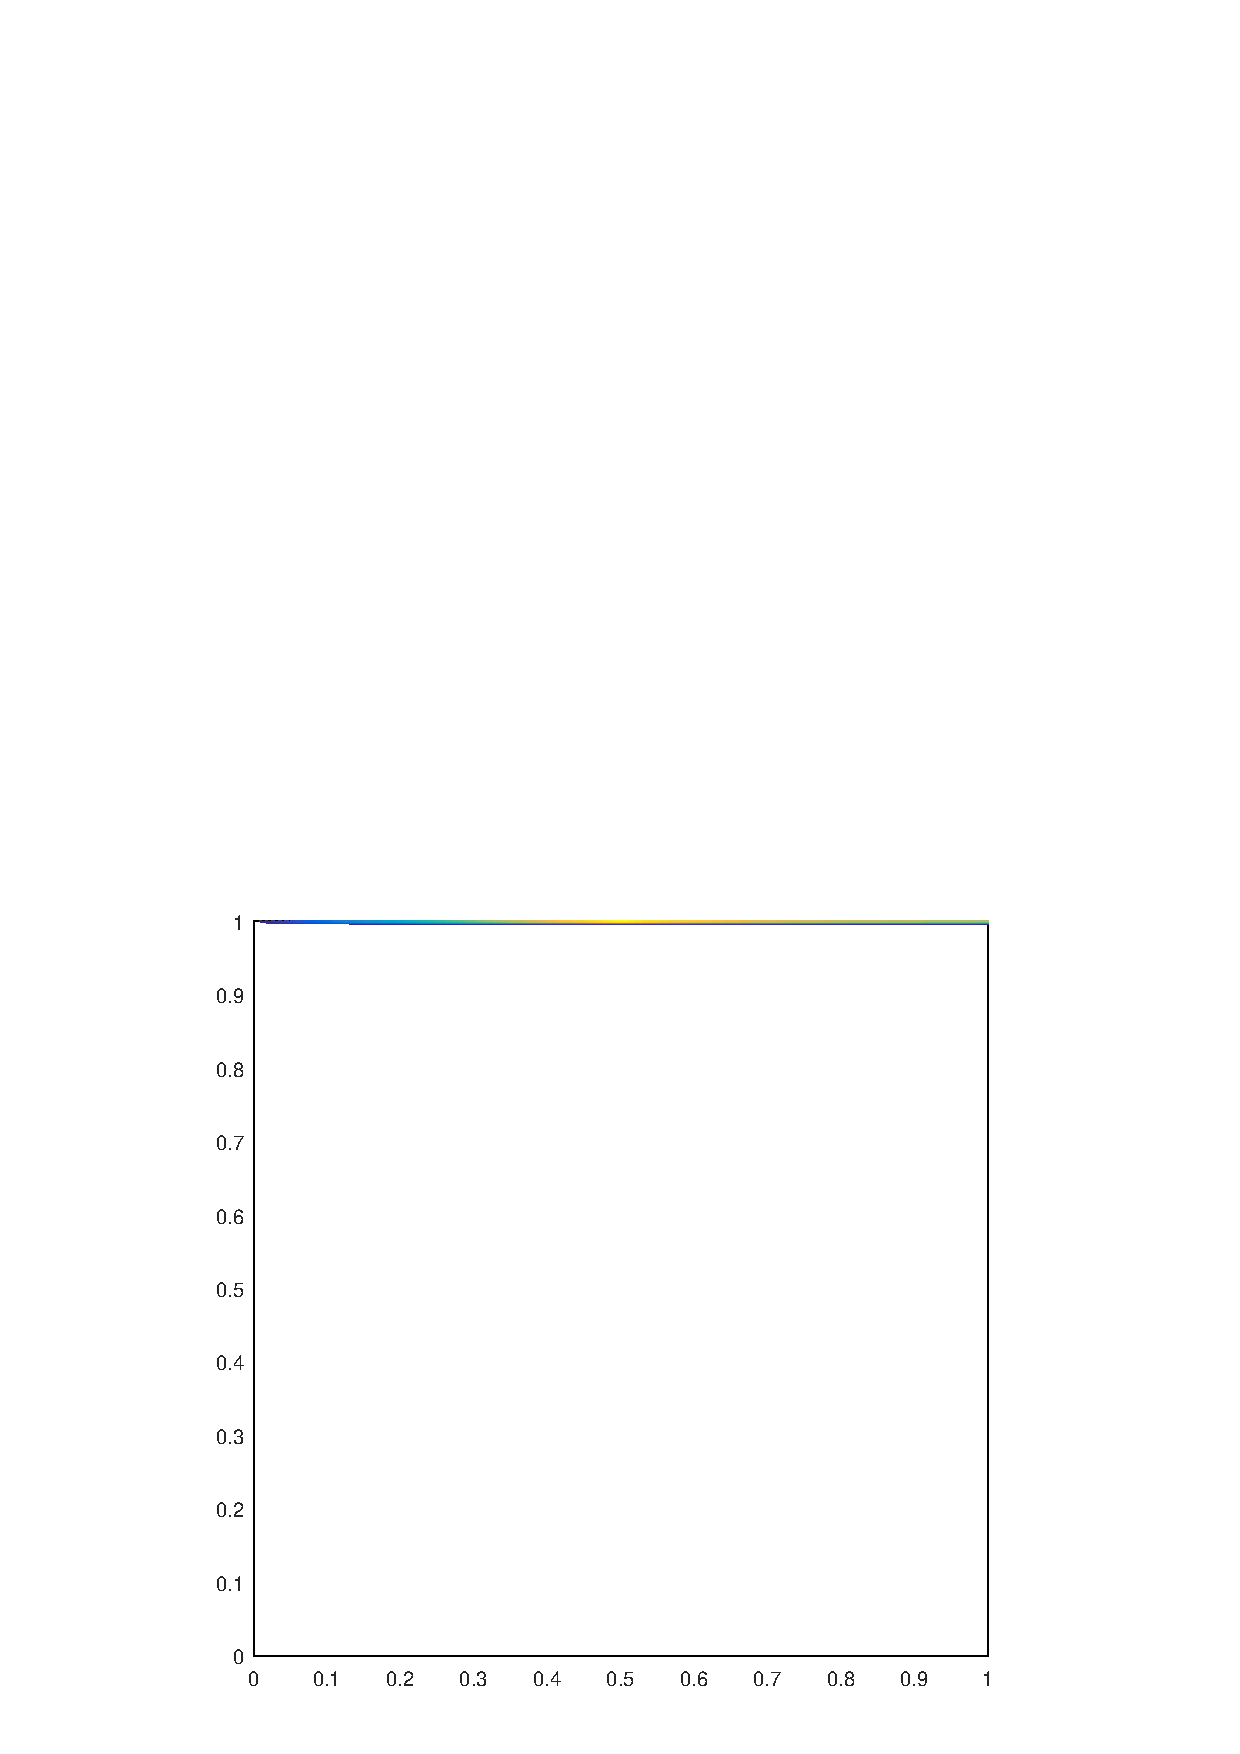
\includegraphics[width=\textwidth]{figures/sec_BF/deg_square_WACHSPRESS1_contour_b4.png}
		\caption{}
	\end{subfigure}
	\vfill
	\begin{subfigure}[b]{0.39\textwidth}
		\centering
		\includegraphics[width=\textwidth]{figures/sec_BF/deg_square_WACHSPRESS1_contour_b5.png}
		\caption{}
	\end{subfigure}
	\hspace{1.5cm}
	\begin{subfigure}[b]{0.39\textwidth}
		\centering
		\includegraphics[width=\textwidth]{figures/sec_BF/deg_square_WACHSPRESS1_contour_b3.png}
		\caption{}
	\end{subfigure}
	\vfill
	\begin{subfigure}[b]{0.39\textwidth}
		\centering
		\includegraphics[width=\textwidth]{figures/sec_BF/deg_square_WACHSPRESS1_contour_b1.png}
		\caption{}
	\end{subfigure}
	\hspace{1.5cm}
	\begin{subfigure}[b]{0.39\textwidth}
		\centering
		\includegraphics[width=\textwidth]{figures/sec_BF/deg_square_WACHSPRESS1_contour_b2.png}
		\caption{}
	\end{subfigure}
\caption{Contour plots of the linear Wachspress basis functions on the degnerate pentagon for the vertices located at: (a) (1/2,1), (b) (0,1), (c) (1,1), (d) (0,0), and (e) (1,0).}
\label{fig::2D_WACHSPRESS1_deg_square_basis_functions}
\end{figure}

%%%%%%%%%%%%%%%%%%%%%%%%%%%%%%%%%%%%%%%%%%%%%%%%%%%
%%%   SubSection - PWL
\subsection{Piecewise Linear (PWL) Basis Functions}
\label{sec::BF_2DLinear_PWL}

The second linearly-complete 2D polygonal coordinates that we will analyze are the Piecewise Linear (PWL) coordinates proposed by Stone and Adams \cite{ref::PWLD_stone_adams,ref::PWLD_stone_adams_unstructured}. They originally introduced the PWL coordinates to work specifically for the DGFEM transport equation on unstructured quadrilateral and polygonal grids. These coordinates share some similarities with the Wachspress rational functions, but also contain some key differences. The properties of the PWL coordinates that are different from the Wachspress rational functions can be summarized with the following:

\begin{enumerate}
\item PWL works with concave polytopes;
\item PWL cannot interpolate on curved surfaces;
\item points on the boundary can be directly evaluated;
\item the PWL integrals can be computed analytically;
\item the PWL functions are only $C^0$ continuous: their gradients are discontinuous within the element.
\end{enumerate}

The 2D PWL functions are defined as combinations of linear triangular functions, with some of them only having measure within a subregion of a polygon. These subregions are formed by triangulating the arbitrary 2D polygon into a set of sub-triangles. Each sub-triangle is defined by two adjacent vertices (taken in a counter-clockwise ordering to maintain consistency) and the polygon's centroid, $\vec{r}_{c}$. Looking at Figure \ref{fig::BF_2D_ref_polygon} as an example, sub-triangle $j$ is defined by the points $\{ \vec{x}_j , \vec{x}_{j+1}, \vec{r}_c \}$, which are the polygon's vertices $j$ and $j+1$ and the polygon's centroid. If a polygon $K$ has $N_K$ vertices, then its centroid can be defined by

\begin{equation}
\label{eq::PWL_2D_centroid}
	\vec{r}_{c} =  \sum\displaylimits_{j=1}^{N_K} \alpha_{j}^{K}  \vec{x}_j ,
\end{equation}

\noindent where $\alpha_{j}^{K}$ are the vertex weights functions and, 

\begin{equation}
\label{eq::PWL_2D_vertex_weight_sum}
 \sum\displaylimits_{j=1}^{N_K} \alpha_{j}^{K} = 1.
\end{equation}

\noindent For this work, we continue to use the definition for the vertex weight functions from previous works \cite{ref::PWLD_stone_adams,ref::PWLD_stone_adams_unstructured,bailey2008phd},

\begin{equation}
\label{eq::PWL_2D_vertex_weight_val}
\alpha_{j}^{K} = \frac{1}{N_K} .
\end{equation}

\noindent This means that the weight functions are equal for every vertex and the cell centroid simply becomes the average position of all the vertices. However, we note that care must be taken so that the centroid does not like on the polygon's boundary. This will cause the PWL functions to no longer have piecewise linearity along the boundary. Using these vertex weight functions, the PWL basis function for vertex $j$, $b_j^{PWL}$, is defined as

\begin{equation}
\label{eq::PWL_2D}
	b_j^{PWL} (x,y) = t_j (x,y) + \alpha_j^K t_c (x,y) .
\end{equation}

\noindent In Eq. (\ref{eq::PWL_2D}), $t_j$ is the standard 2D linear function with unity at vertex $j$ that linearly decreases to zero to the cell center and each adjoining vertex. $t_c$ is the 2D cell ``tent'' function located at $\vec{r}_{c}$ which is unity at the cell center and linearly decreases to zero to each cell vertex. $\alpha_{j}^{K}$ is the weight parameter for vertex $j$ in cell $K$. The functional form of Eq. (\ref{eq::PWL_2D}) with constant vertex weights means that the PWL function for vertex $j$, within the domain of $K$, linearly decreases to a value of $1/N_K$ at the polygonal center. From there, the function linearly decreases to zero on all faces that are not connected to vertex $j$. The gradients of the PWL functions are easy to compute term-by-term in a straightforward manner:

\begin{equation}
\label{eq::PWL_2D_gradients}
	\vec{\nabla} b_j^{PWL} (x,y) = \vec{\nabla} t_j (x,y) + \alpha_j^K \vec{\nabla} t_c (x,y) .
\end{equation}

We now give some example contour plots of the PWL coordinates over different polygons. First, we provide the contour plots for the four PWL functions on the unit square in Figure \ref{fig::2D_PWLD1_unit_square_basis_functions}. In this example it is easy to discern the functional form of Eq. (\ref{eq::PWL_2D}) with the use of constant vertex weights. We clearly see each function linearly decrease from its vertex to the cell center (with a value of $1/N_K$) and then linearly decrease to all non-adjoining faces. Next, Figure \ref{fig::2D_PWLD1_deg_square_basis_functions} provides the contour plots for the PWL functions on a degenerate (weakly-convex) pentagon where a fifth vertex was added to the unit square at ($1/2,1$). Unlike the Wachspress coordinates, the PWL functions work on weakly-convex polygons. The final example we give in Figure \ref{fig::2D_PWLD1_Ldom_basis_functions} is a favorite in the applied mathematics community: the ``L-shaped'' domain. It provides an example of PWL's ability to still be linearly-complete on concave polygons. In this example, the cell centroid was forced to be at the point ($1/3,1/3$) so that it would be inside of the polygon.


\begin{figure}
\centering
	\begin{subfigure}[b]{0.39\textwidth}
		\centering
		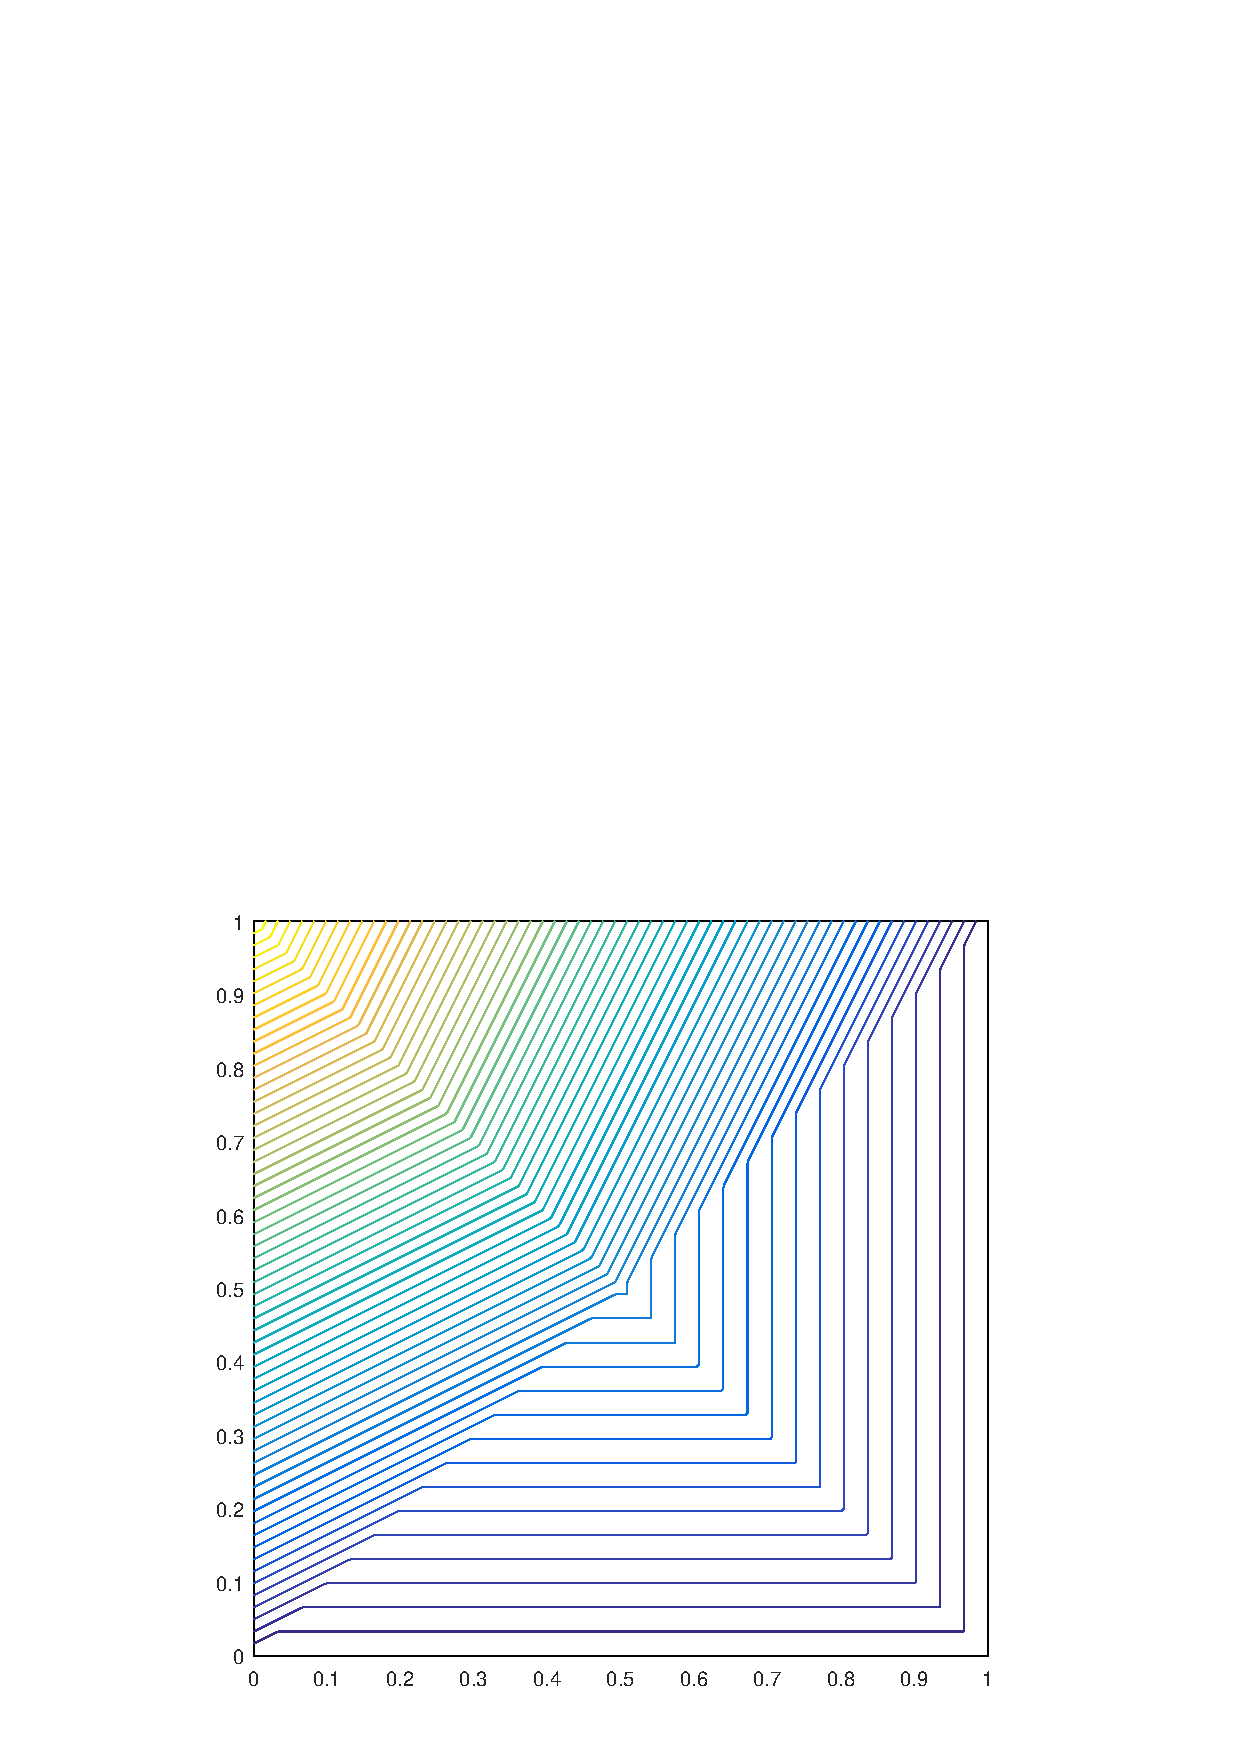
\includegraphics[width=\textwidth]{figures/sec_BF/square_PWLD1_contour_b4.png}
		\caption{}
	\end{subfigure}
	\hspace{1.5cm}
	\begin{subfigure}[b]{0.39\textwidth}
		\centering
		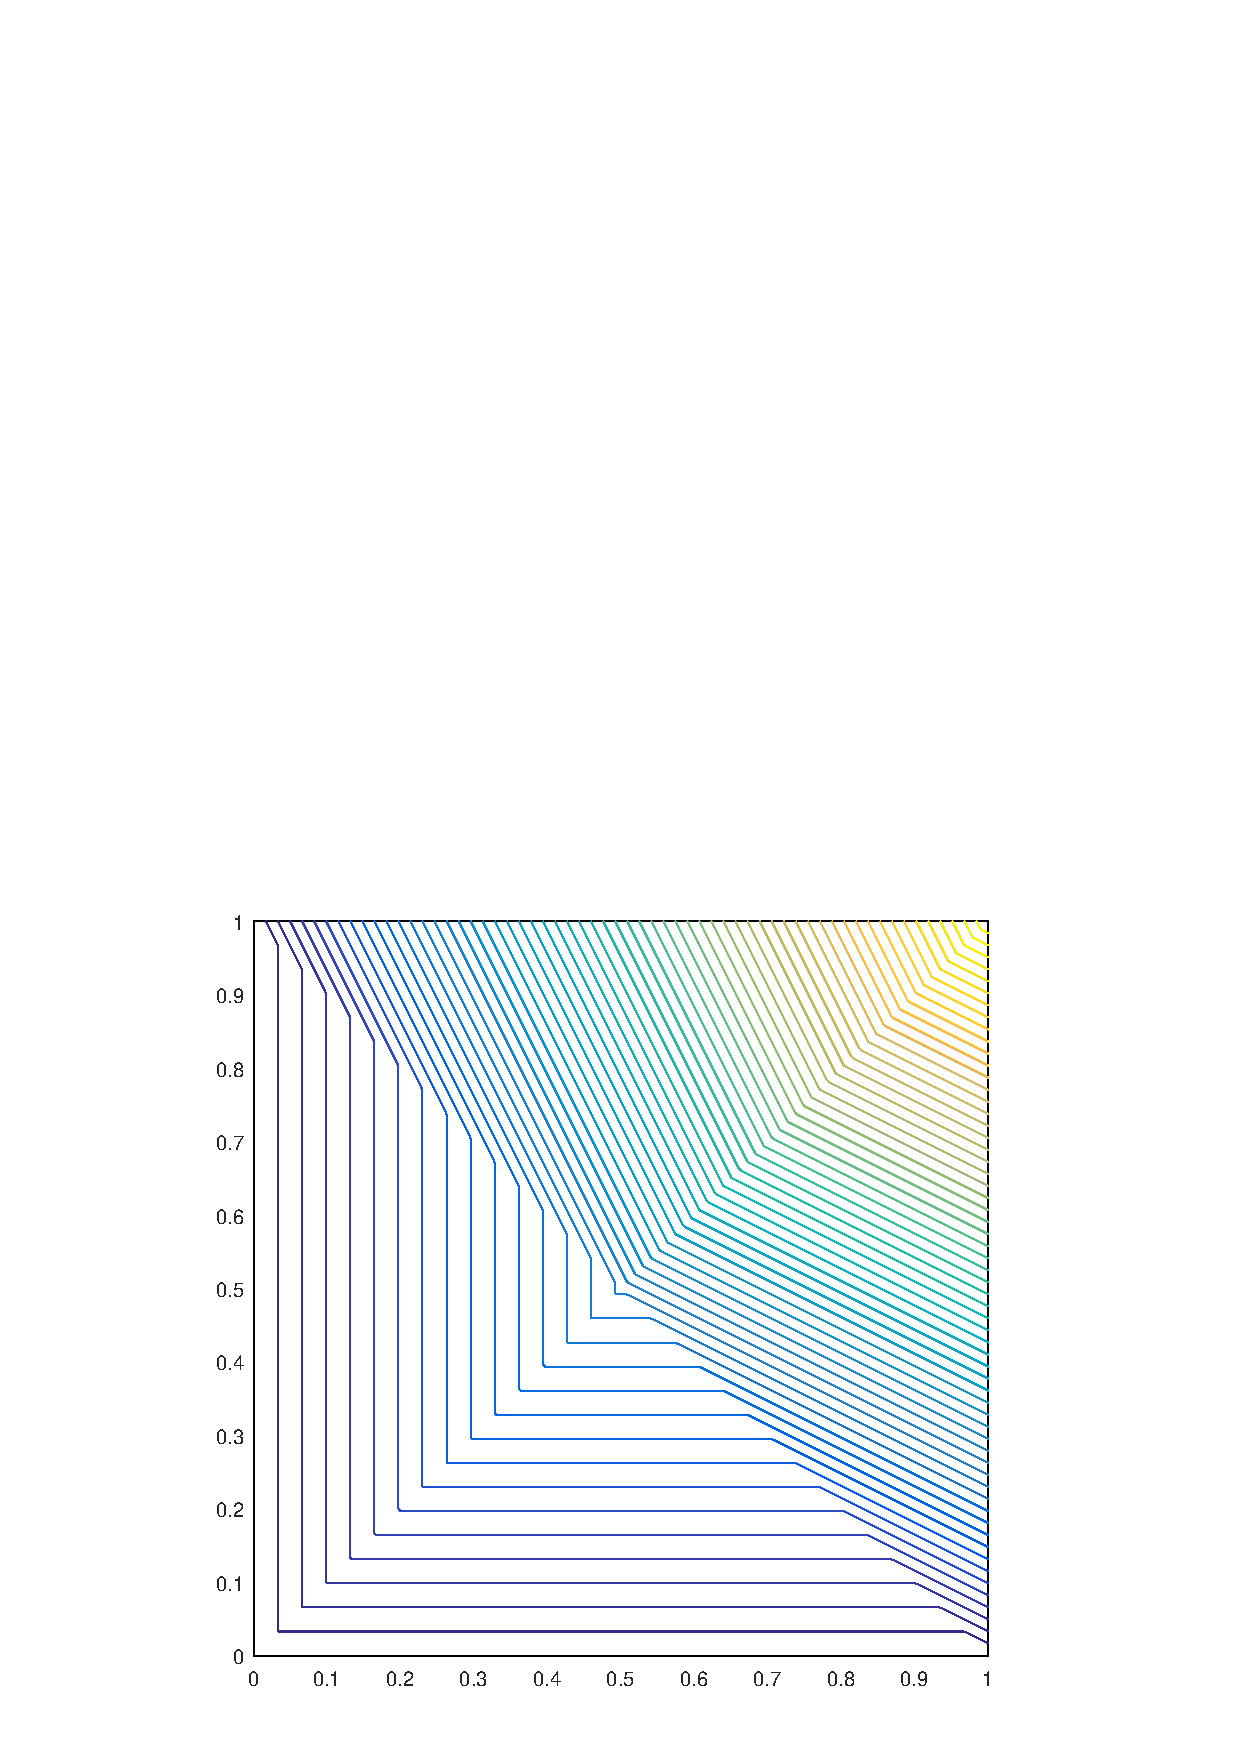
\includegraphics[width=\textwidth]{figures/sec_BF/square_PWLD1_contour_b3.png}
		\caption{}
	\end{subfigure}
	\vfill
	\begin{subfigure}[b]{0.39\textwidth}
		\centering
		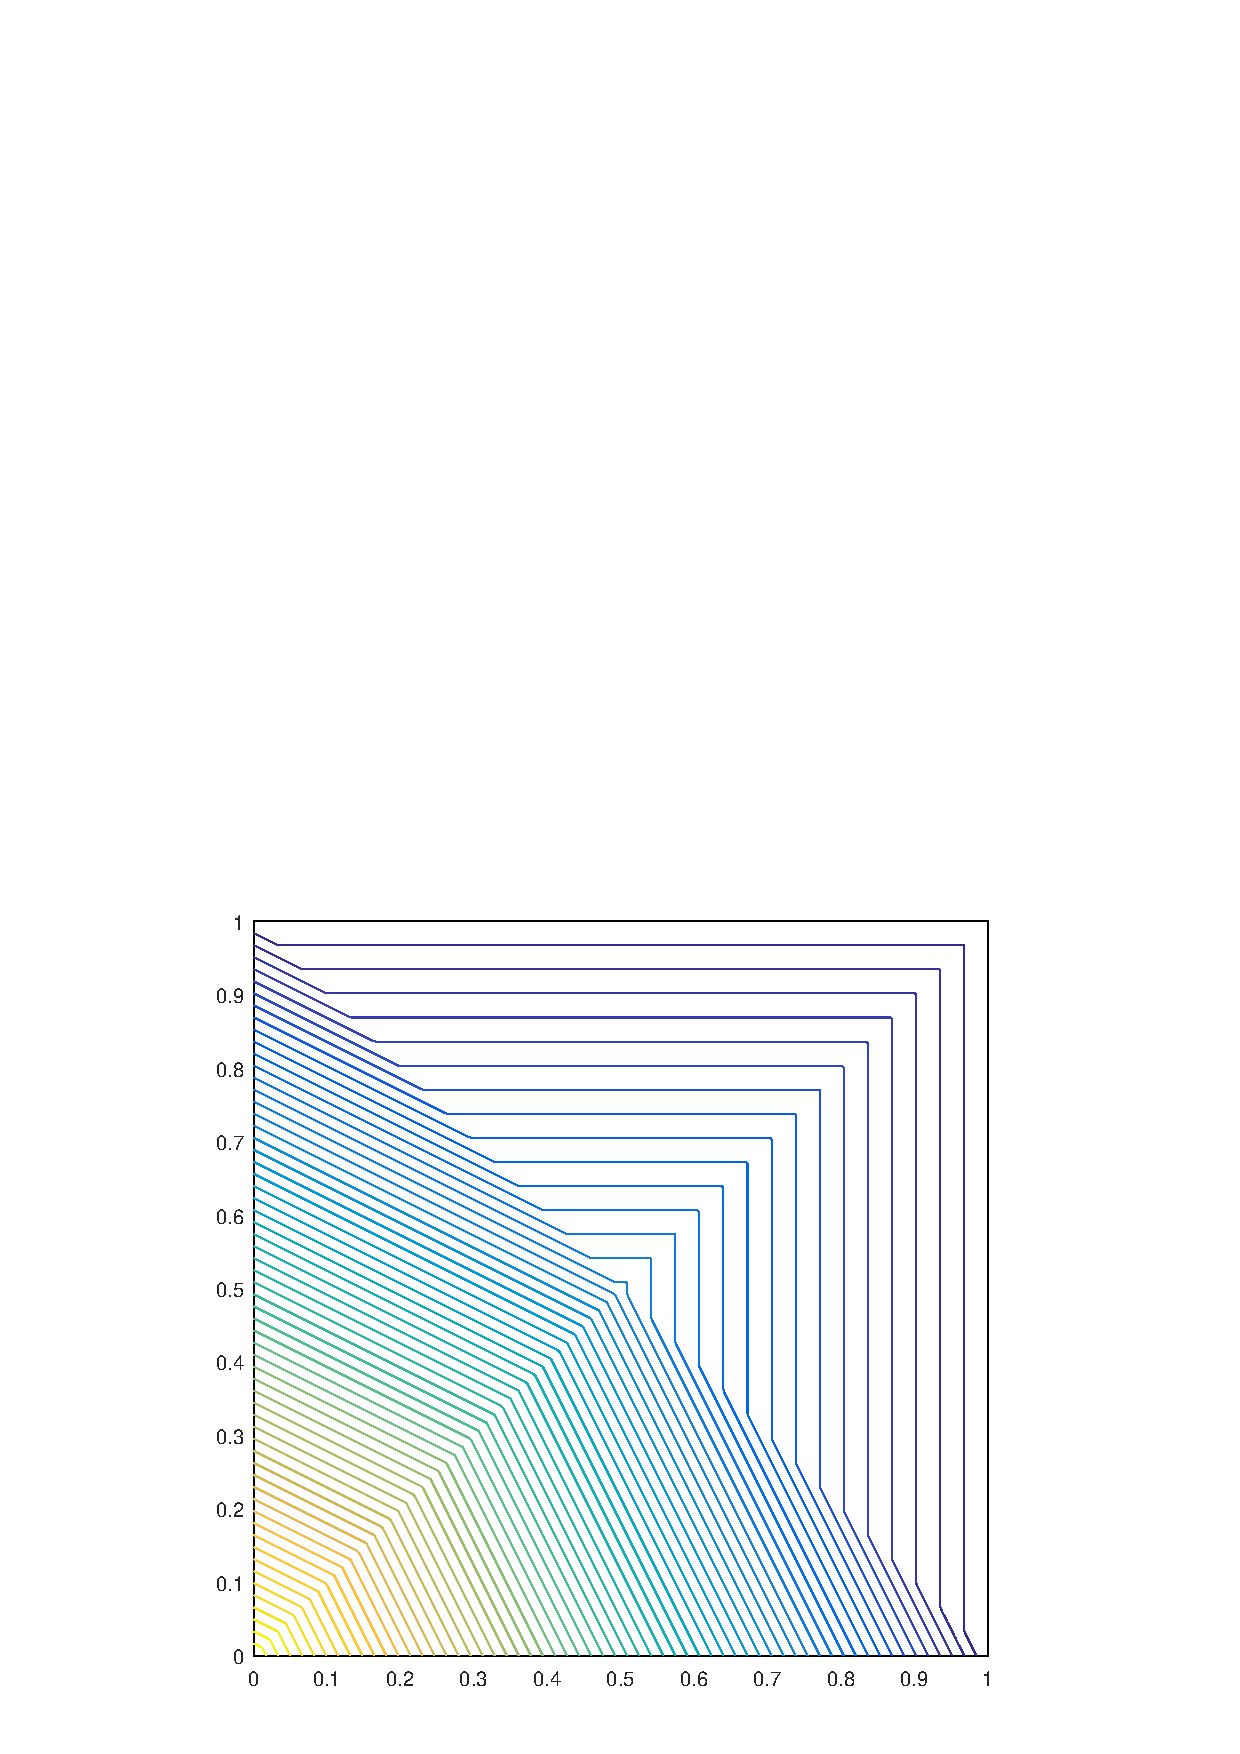
\includegraphics[width=\textwidth]{figures/sec_BF/square_PWLD1_contour_b1.png}
		\caption{}
	\end{subfigure}
	\hspace{1.5cm}
	\begin{subfigure}[b]{0.39\textwidth}
		\centering
		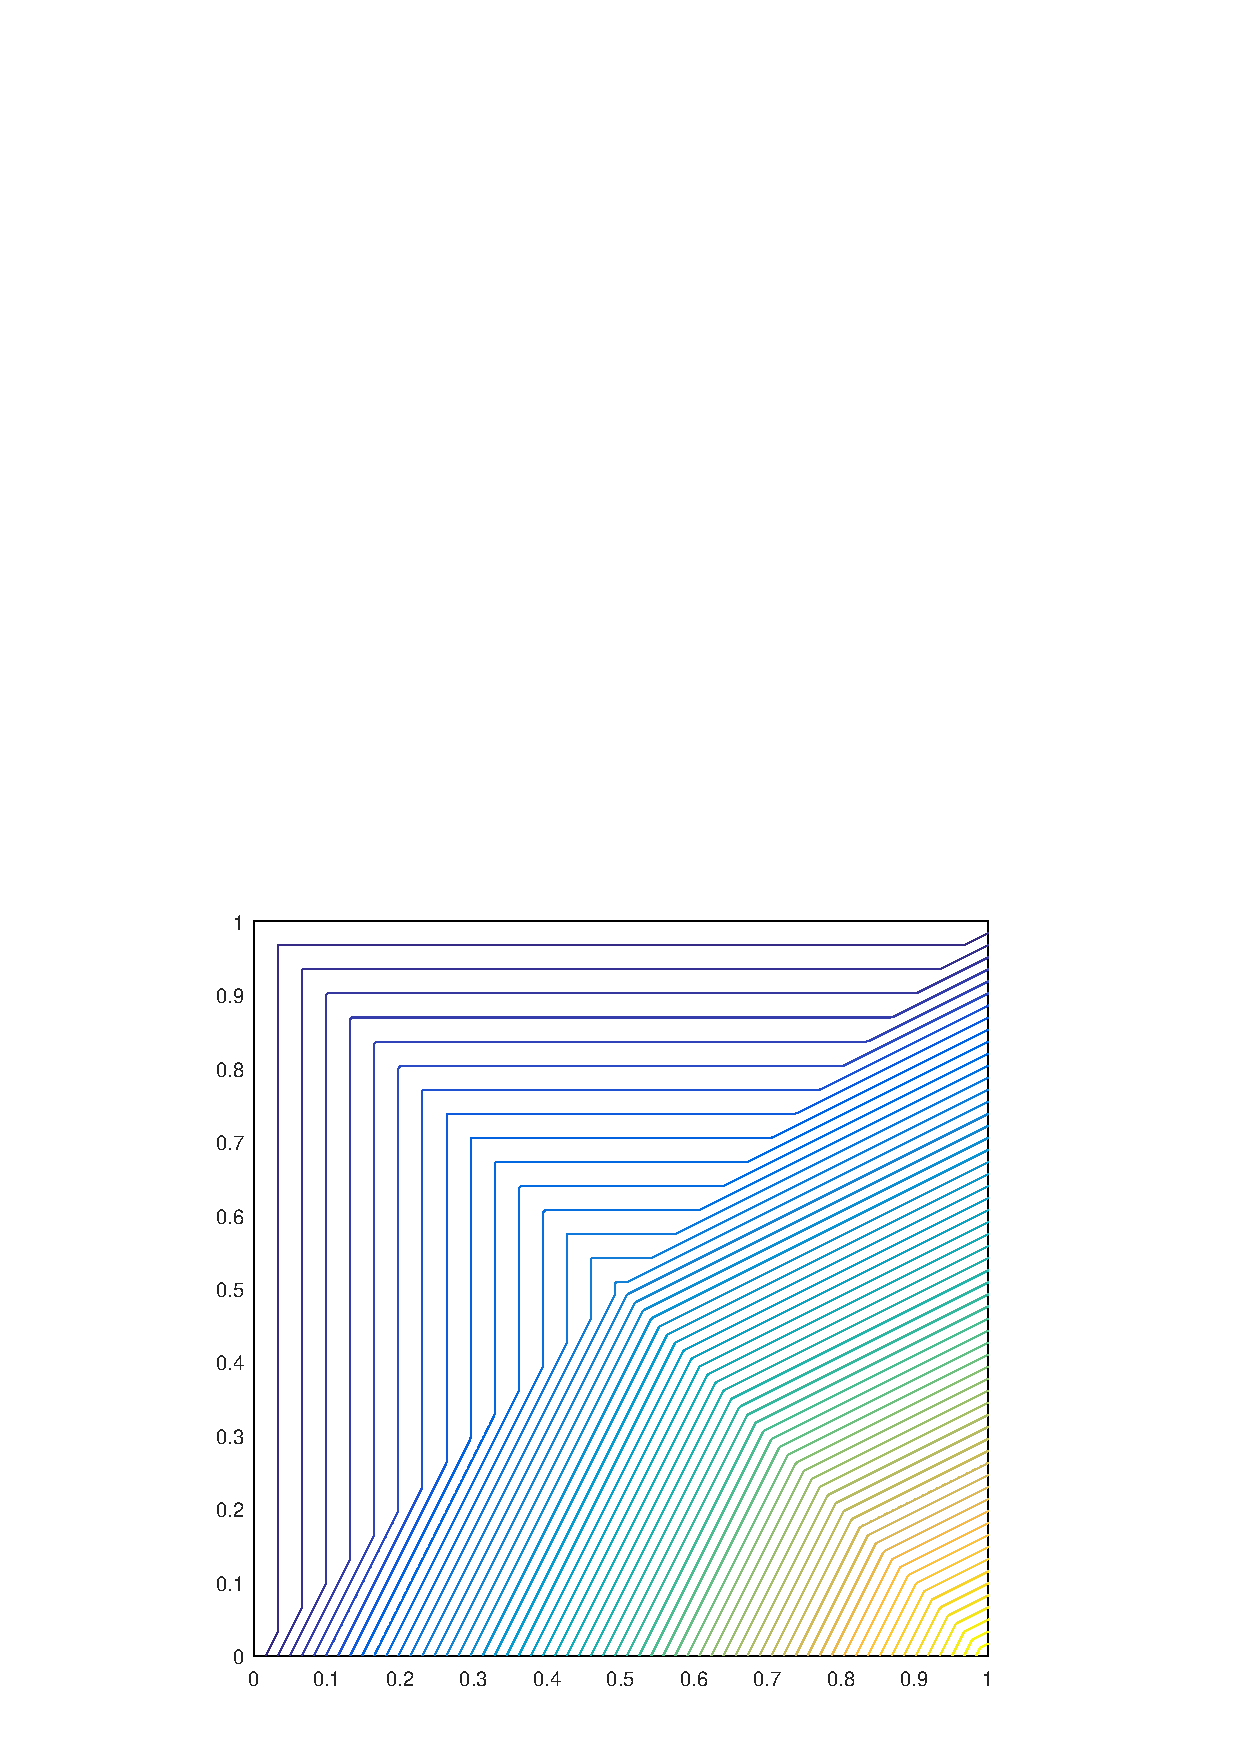
\includegraphics[width=\textwidth]{figures/sec_BF/square_PWLD1_contour_b2.png}
		\caption{}
	\end{subfigure}
\caption{Contour plots of the linear PWL basis functions on the unit square for the vertices located at: (a) (0,1), (b) (1,1), (c) (0,0), and (d) (1,0).}
\label{fig::2D_PWLD1_unit_square_basis_functions}
\end{figure}

\begin{figure}
\centering
	\begin{subfigure}[b]{0.39\textwidth}
		\centering
		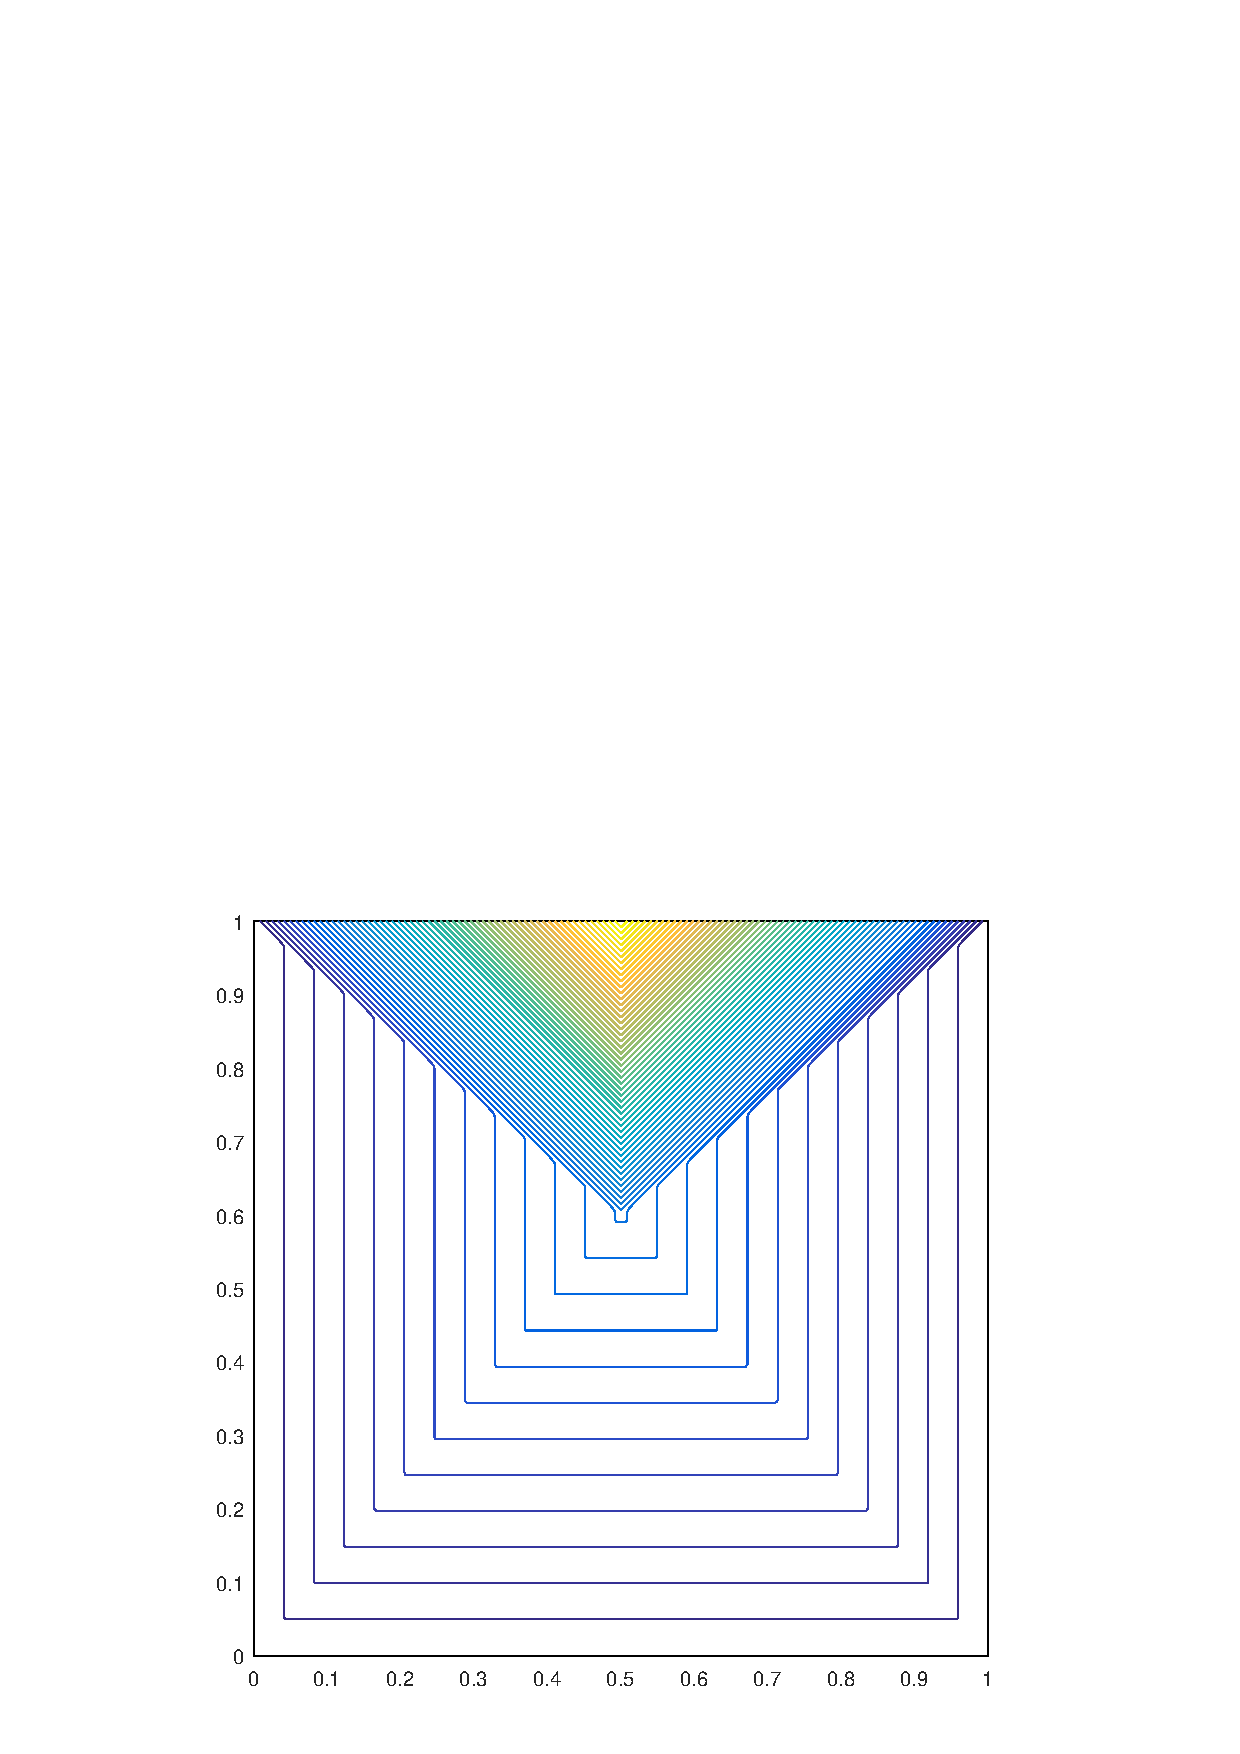
\includegraphics[width=\textwidth]{figures/sec_BF/deg_square_PWLD1_contour_b4.png}
		\caption{}
	\end{subfigure}
	\vfill
	\begin{subfigure}[b]{0.39\textwidth}
		\centering
		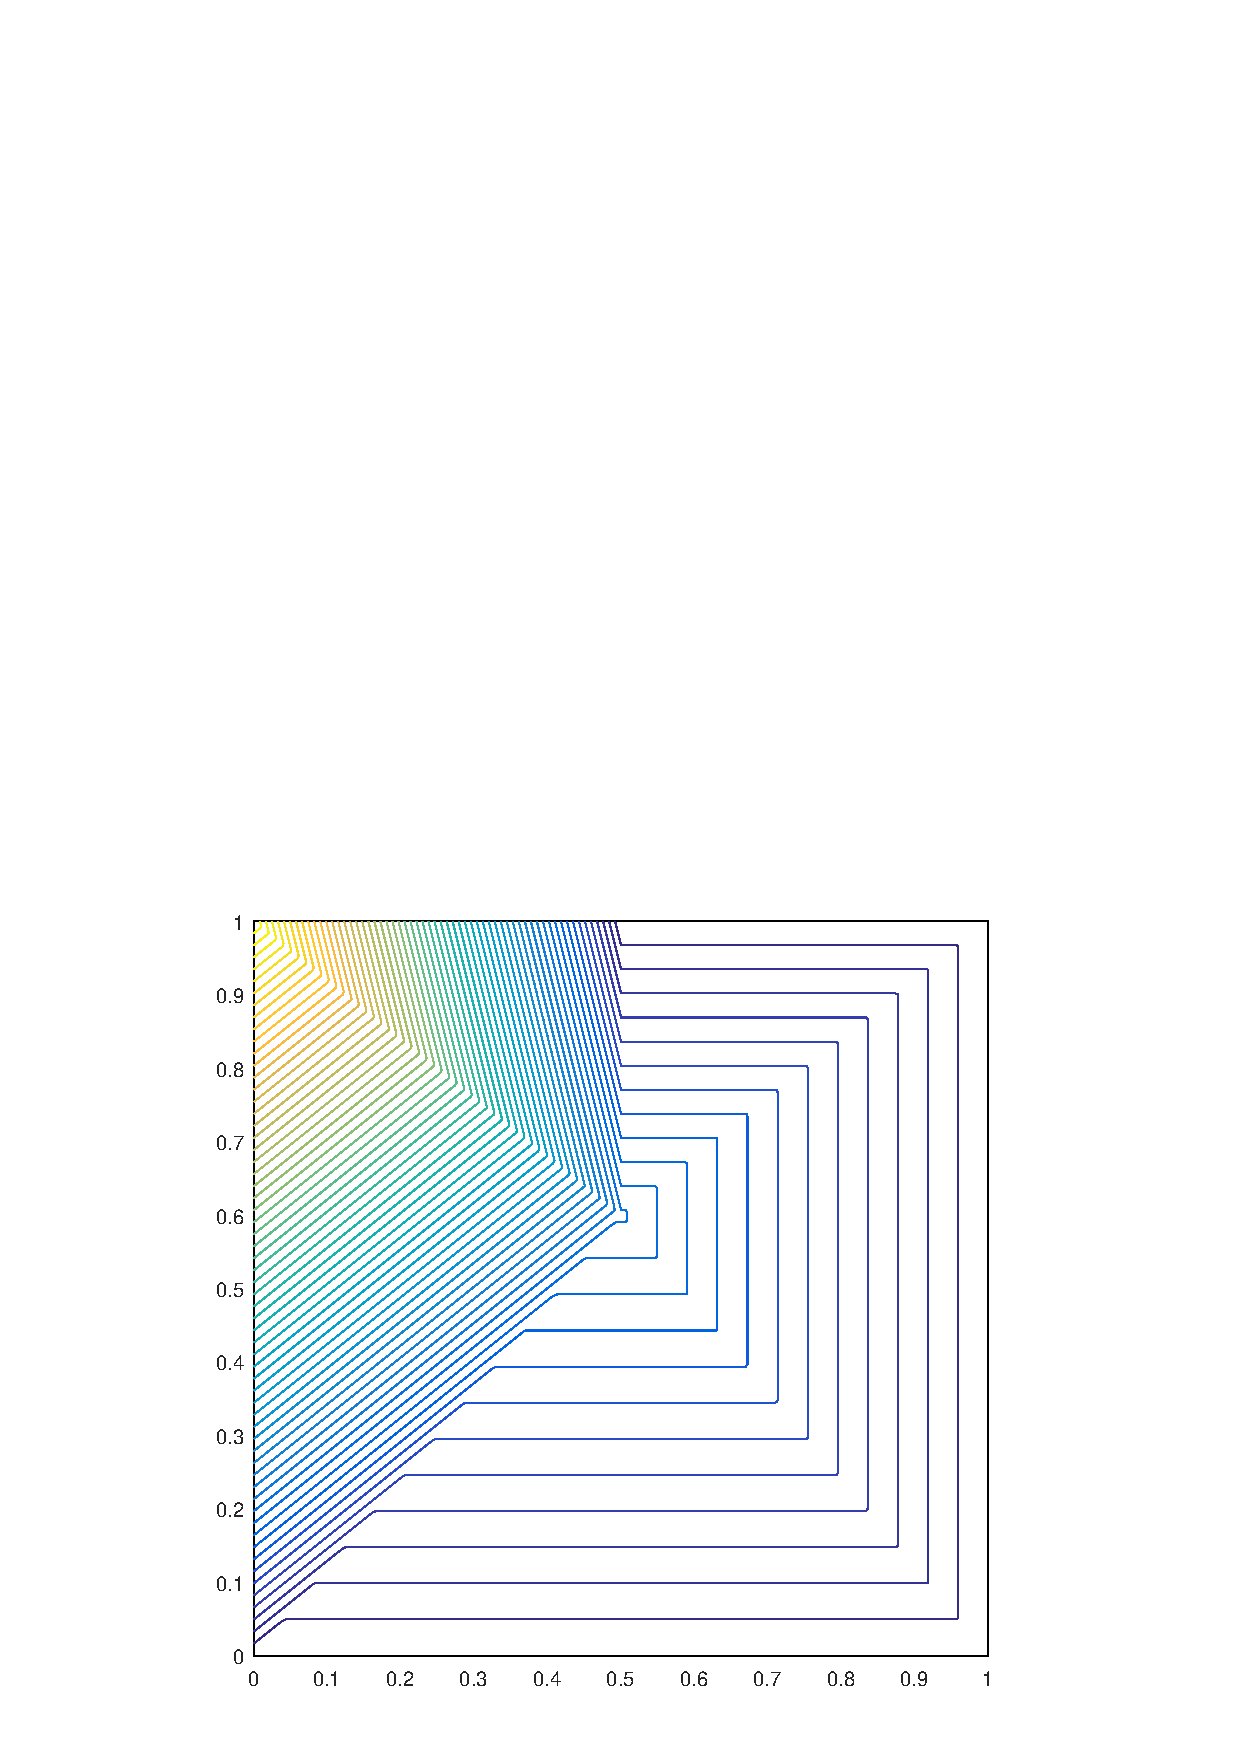
\includegraphics[width=\textwidth]{figures/sec_BF/deg_square_PWLD1_contour_b5.png}
		\caption{}
	\end{subfigure}
	\hspace{1.5cm}
	\begin{subfigure}[b]{0.39\textwidth}
		\centering
		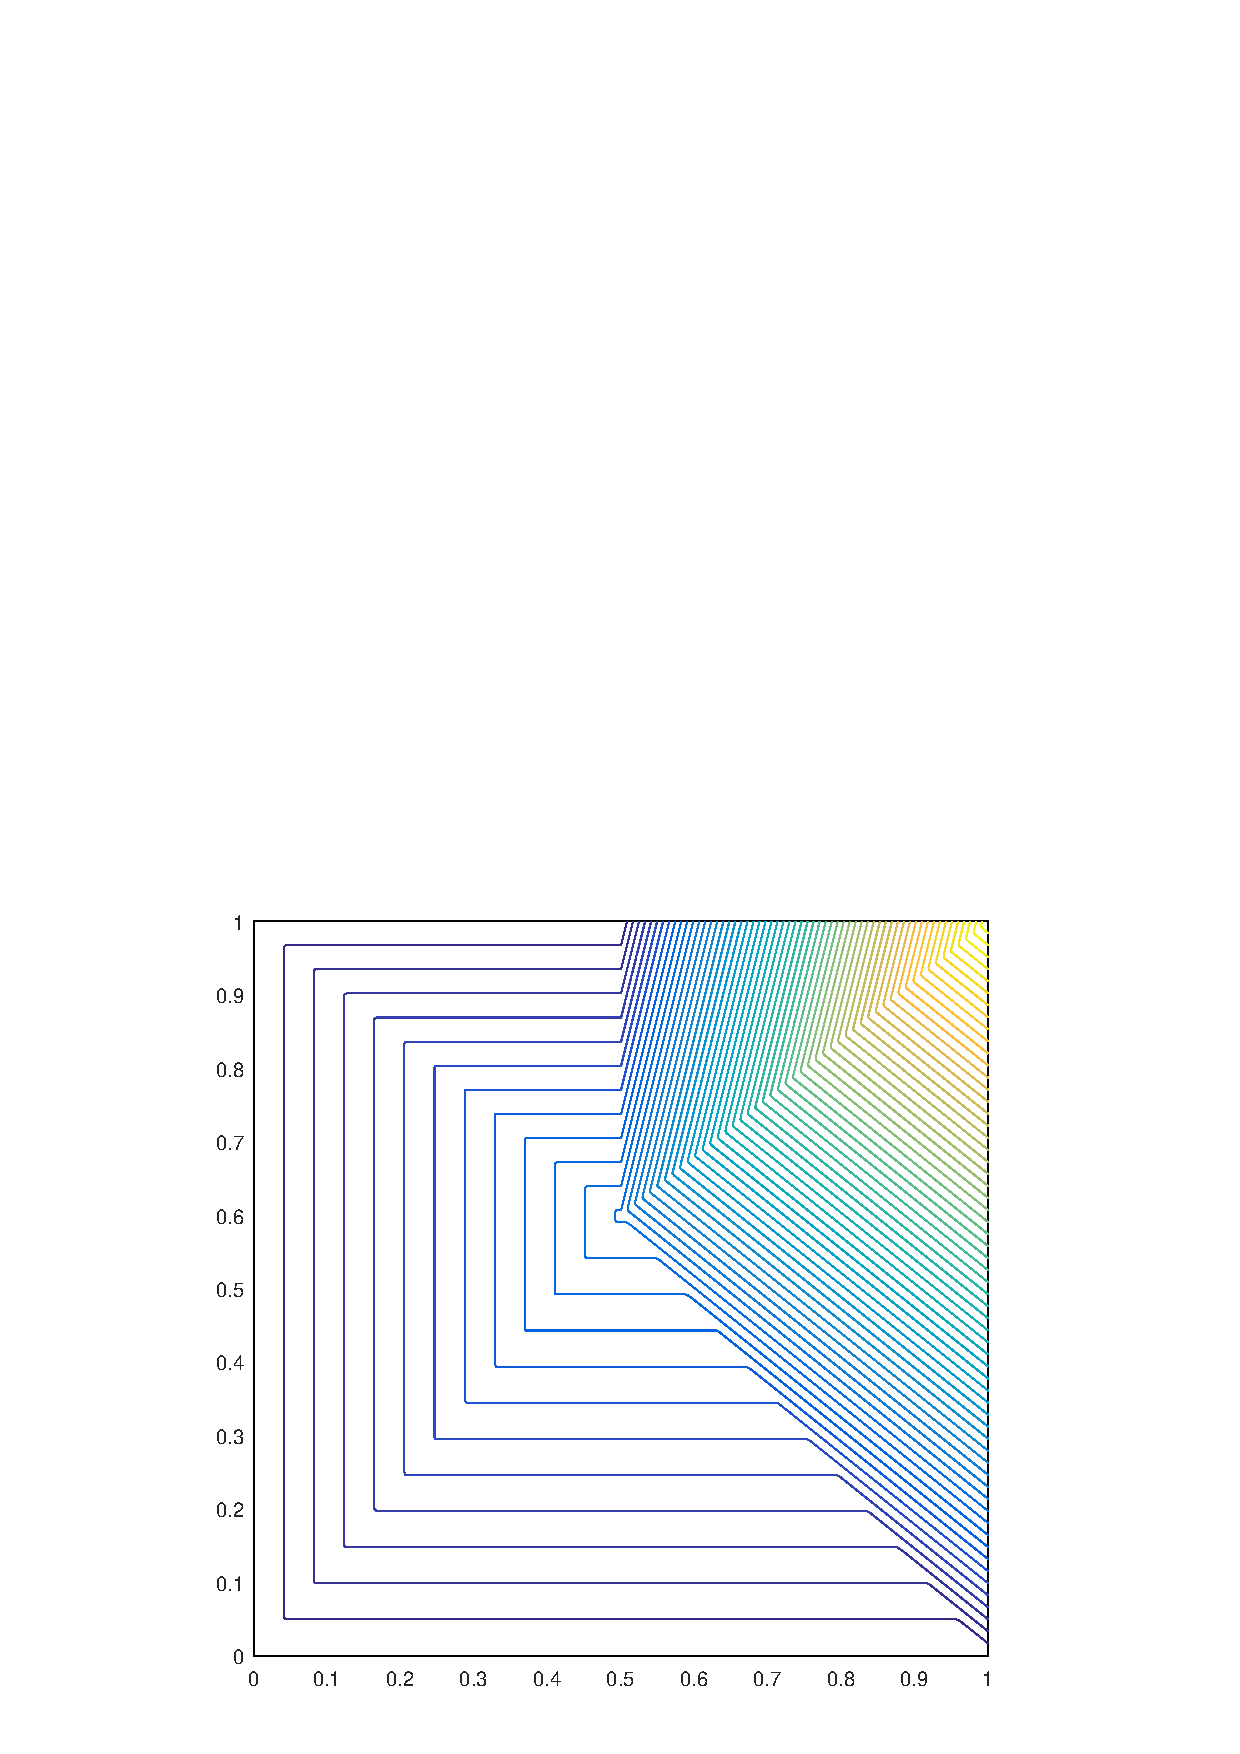
\includegraphics[width=\textwidth]{figures/sec_BF/deg_square_PWLD1_contour_b3.png}
		\caption{}
	\end{subfigure}
	\vfill
	\begin{subfigure}[b]{0.39\textwidth}
		\centering
		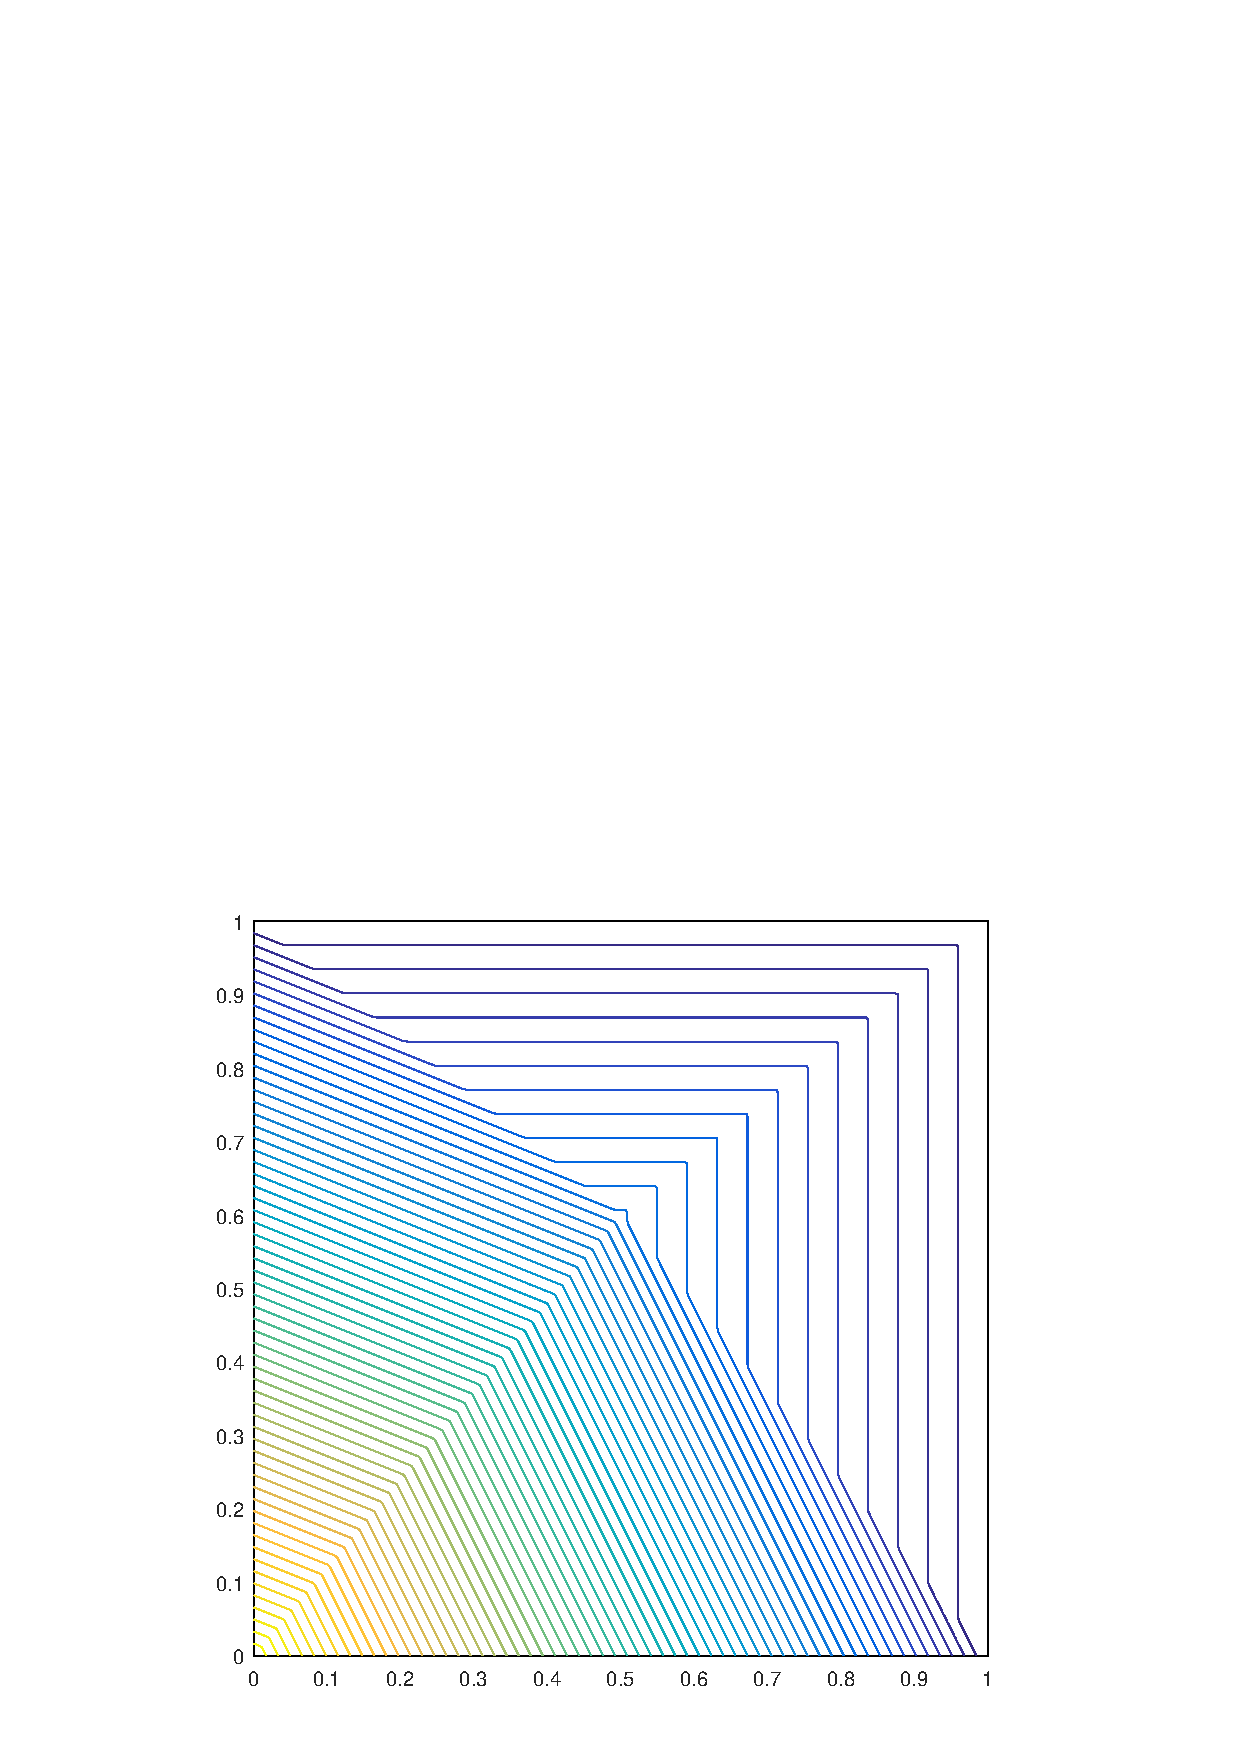
\includegraphics[width=\textwidth]{figures/sec_BF/deg_square_PWLD1_contour_b1.png}
		\caption{}
	\end{subfigure}
	\hspace{1.5cm}
	\begin{subfigure}[b]{0.39\textwidth}
		\centering
		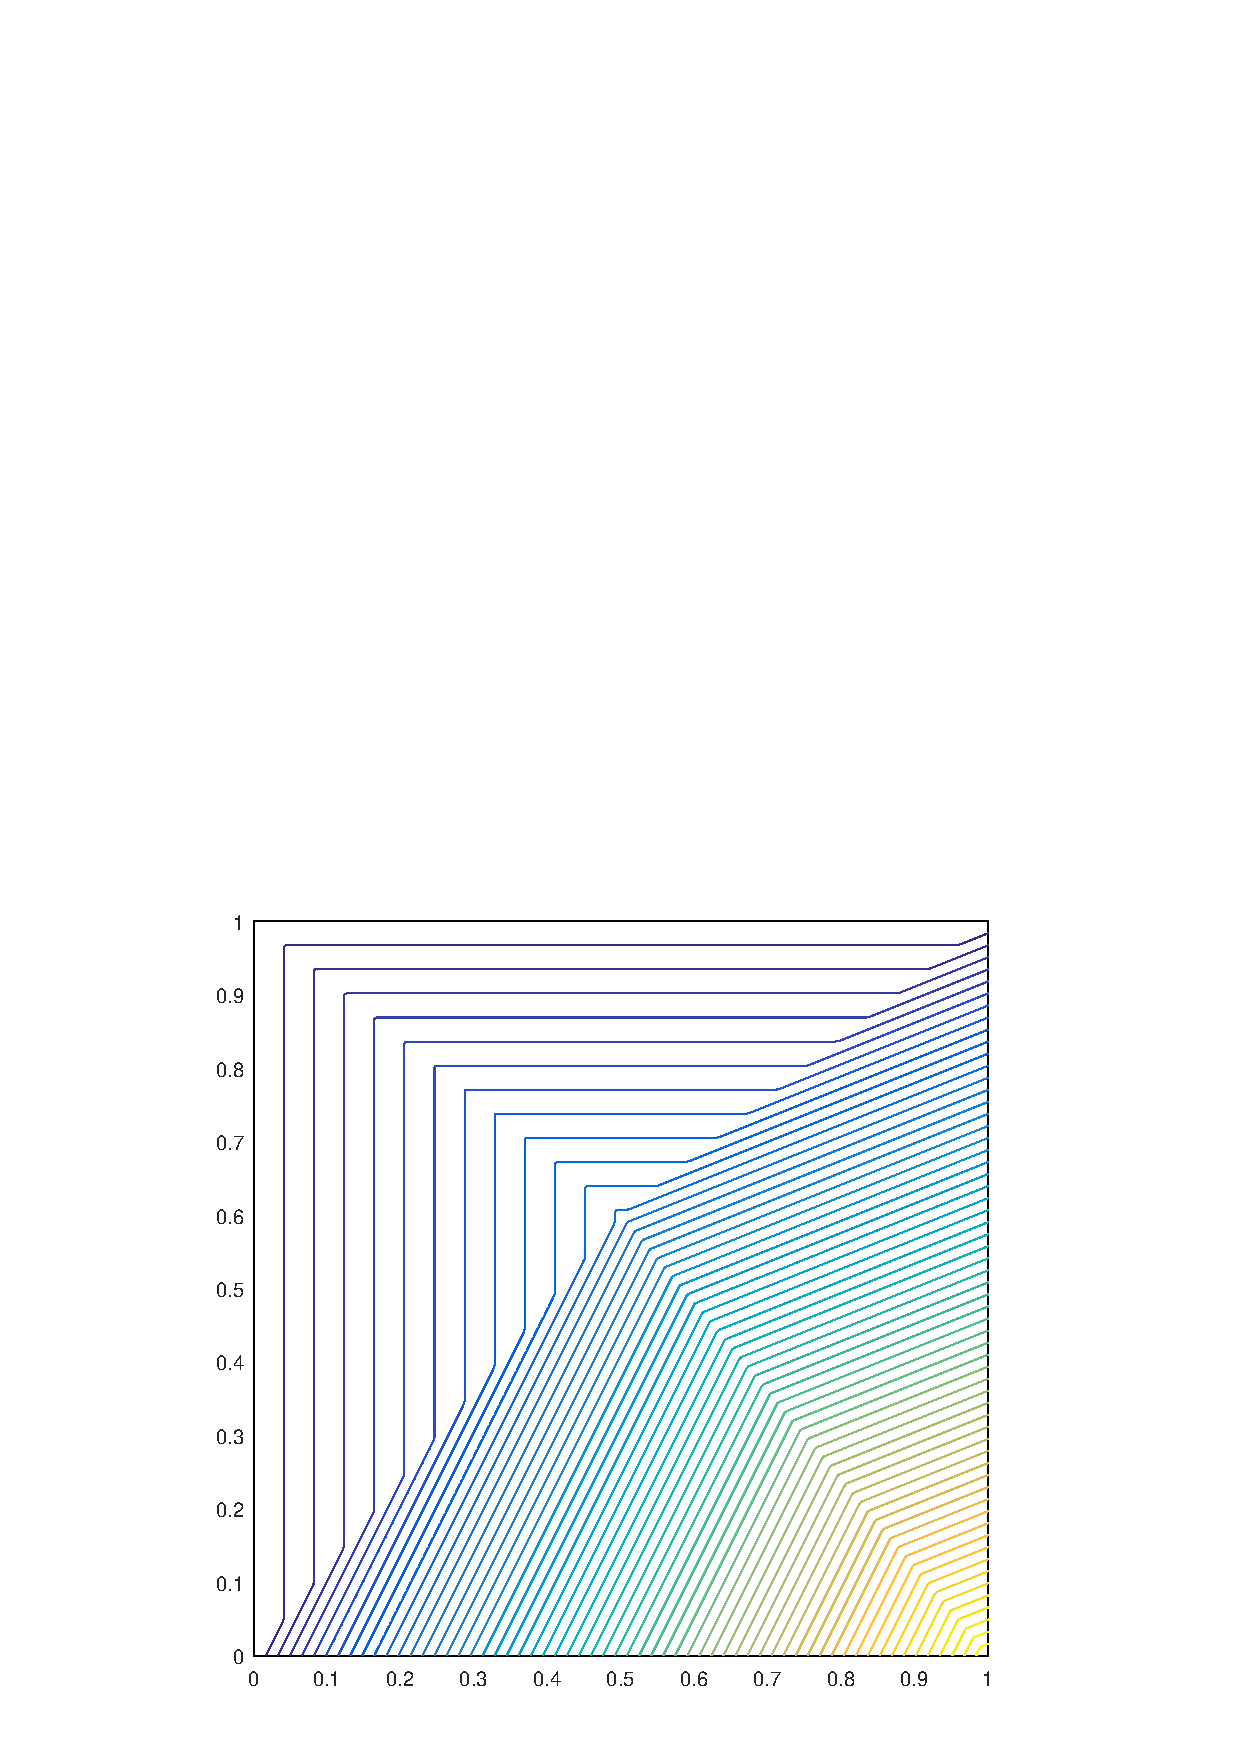
\includegraphics[width=\textwidth]{figures/sec_BF/deg_square_PWLD1_contour_b2.png}
		\caption{}
	\end{subfigure}
\caption{Contour plots of the linear PWL basis functions on the degnerate pentagon for the vertices located at: (a) (1/2,1), (b) (0,1), (c) (1,1), (d) (0,0), and (e) (1,0).}
\label{fig::2D_PWLD1_deg_square_basis_functions}
\end{figure}

\begin{figure}
\centering
	\begin{subfigure}[b]{0.39\textwidth}
		\centering
		\includegraphics[width=\textwidth]{figures/sec_BF/L-domain_PWLD1_contour_b6.png}
		\caption{}
	\end{subfigure}
	\hspace{1.5cm}
	\begin{subfigure}[b]{0.39\textwidth}
		\centering
		\includegraphics[width=\textwidth]{figures/sec_BF/L-domain_PWLD1_contour_b5.png}
		\caption{}
	\end{subfigure}
	\vfill
	\begin{subfigure}[b]{0.39\textwidth}
		\centering
		\includegraphics[width=\textwidth]{figures/sec_BF/L-domain_PWLD1_contour_b4.png}
		\caption{}
	\end{subfigure}
	\hspace{1.5cm}
	\begin{subfigure}[b]{0.39\textwidth}
		\centering
		\includegraphics[width=\textwidth]{figures/sec_BF/L-domain_PWLD1_contour_b3.png}
		\caption{}
	\end{subfigure}
	\vfill
	\begin{subfigure}[b]{0.39\textwidth}
		\centering
		\includegraphics[width=\textwidth]{figures/sec_BF/L-domain_PWLD1_contour_b1.png}
		\caption{}
	\end{subfigure}
	\hspace{1.5cm}
	\begin{subfigure}[b]{0.39\textwidth}
		\centering
		\includegraphics[width=\textwidth]{figures/sec_BF/L-domain_PWLD1_contour_b2.png}
		\caption{}
	\end{subfigure}
\caption{Contour plots of the linear PWL basis functions on the L-shaped domain for the vertices located at: (a) (0,1), (b) (1/2,1), (c) (1/2,1/2), (d) (1,1/2), (e) (0,0), and (f) (1,0).}
\label{fig::2D_PWLD1_Ldom_basis_functions}
\end{figure}





%%%%%%%%%%%%%%%%%%%%%%%%%%%%%%%%%%%%%%%%%%%%%%%%%%%
%%%   SubSection - Mean Value
\subsection{Mean Value Basis Functions}
\label{sec::BF_2DLinear_MV}

At this point, we now introduce the first new polygonal basis set for use with the transport equation: the {\em mean value coordinates} (MV) developed by Floater \cite{floater2003mean,hormann2006mean}. The original motivation behind the MV coordinates was to approximate harmonic maps on a polygon by a set of piecewise linear maps over a triangulation of the polygon for use in computer aided graphic design. Injectivity is preserved if the interpolatory function is {\em harmonic} over the piecewise linear maps. This can be shown by expressing a $C^2$ function $u$ over each sub-triangle of the triangulated polygon and have it statisfy the Laplace equation,

\begin{equation}
\label{eq::BF_MV_laplace}
\nabla^2 u = 0 ,
\end{equation}

\noindent where $u(\vec{r}) = u_0$ constituting a piecewise linear function 

\begin{equation}
\label{eq::BF_MV_BF}
b_{j}^{MV} (\vec{x}) = \frac{w_j (\vec{x}) }{\sum_i w_i (\vec{x})}
\end{equation}

\noindent where the mean value weight function for vertex $j$, $w_j$, has the following definition:

\begin{equation}
\label{eq::BF_MV_weights}
w_j (\vec{x})  = \frac{\tan(\alpha_{j-1} / 2) + \tan(\alpha_j / 2)}{|\vec{x}_j - \vec{x}|}
\end{equation}

We now give the form of the mean value gradients. Since the mean value coordinates given by Eq. (\ref{eq::BF_MV_BF}) have the same form as the Wachspress coodinates, their gradients can be expressed in an indentical manner. The gradients of the mean value coordinates can be expressed as

\begin{equation}
\label{eq::BF_mv_gradient}
\vec{\nabla} b_{j}^{MV}(\vec{x}) = b_{j}^{MV} (\vec{x}) \left( \vec{R}_j  (\vec{x})- \sum\displaylimits_{i}   b_{i}^{MV} (\vec{x}) \vec{R}_i (\vec{x}) \right) ,
\end{equation}

\noindent where the reduced gradient, $\vec{R}_j $, still has the same definition from Eq. (\ref{eq::BF_wach_reduced_grad}). If we define $t_j=\tan(\alpha_j/2)$ and $t_{j-1}=\tan(\alpha_{j-1}/2)$, then after extensive algebra, the mean value reduced gradients are

\begin{equation}
\label{eq::BF_mv_red_grad_form}
\vec{R}_j  = \left( \frac{t_{j-1}}{t_{j-1} + t_{j}} \right) \frac{\{  \vec{c}_{j-1} \}}{\sin (  \alpha_{j-1} )} +  \left( \frac{t_{j}}{t_{j-1} + t_{j}} \right) \frac{\{  \vec{c}_{j} \}}{\sin (  \alpha_{j} )}+ \frac{\vec{g}_j}{|\vec{x}_i - \vec{x}|},
\end{equation}

\noindent where

\begin{equation}
\label{eq::BF_mv_red_cval}
\vec{c}_j = \frac{\vec{g}_{j}}{|\vec{x}_j - \vec{x}|} - \frac{\vec{g}_{j+1}}{|\vec{x}_{j+1} - \vec{x}|},
\end{equation}

\noindent and

\begin{equation}
\label{eq::BF_mv_red_gval}
\vec{g}_j = \frac{\vec{x}_j - \vec{x}}{|\vec{x}_j - \vec{x}|},
\end{equation}

\noindent and 

\begin{equation}
\label{eq::BF_mv_red_flop}
\{  \vec{u} \} = \left( - u_2 , u_1  \right). 
\end{equation}

\noindent While this direct form for the MV coordinates is more complicated than the last two coordinates presented, it is still easily programmable. The interested reader can look in the appendix of \cite{floater2015generalized} for MATLAB code to compute these gradients, though we stress that it does not contain any logic for boundary detection.

We again provide example contour plots of the MV coordinates, and we use the same polygonal shapes that we showed for the PWL coordinates. Figure \ref{fig::2D_MV1_unit_square_basis_functions} gives the MV coordinates on the unit square. Like the Wachspress functions, the MV coordinates are smoothly varying within the domain of the polygon and posess continuous derivatives. Next in Figure \ref{fig::2D_MV1_deg_square_basis_functions}, we give the example contour plots for the degenerate pentagon which is formed by inserting a vertex into the unit square at $(1/2,1)$. Finally, Figure \ref{fig::2D_MV1_Ldom_basis_functions} gives the contour plots for the linear mean value coordinates on the L-shaped domain. We see that the linear mean value coordinates are applicable to interpolation on concave polygons.

\begin{figure}
\centering
	\begin{subfigure}[b]{0.39\textwidth}
		\centering
		\includegraphics[width=\textwidth]{figures/sec_BF/square_MV1_contour_b4.png}
		\caption{}
	\end{subfigure}
	\hspace{1.5cm}
	\begin{subfigure}[b]{0.39\textwidth}
		\centering
		\includegraphics[width=\textwidth]{figures/sec_BF/square_MV1_contour_b3.png}
		\caption{}
	\end{subfigure}
	\vfill
	\begin{subfigure}[b]{0.39\textwidth}
		\centering
		\includegraphics[width=\textwidth]{figures/sec_BF/square_MV1_contour_b1.png}
		\caption{}
	\end{subfigure}
	\hspace{1.5cm}
	\begin{subfigure}[b]{0.39\textwidth}
		\centering
		\includegraphics[width=\textwidth]{figures/sec_BF/square_MV1_contour_b2.png}
		\caption{}
	\end{subfigure}
\caption{Contour plots of the linear mean value basis functions on the unit square for the vertices located at: (a) (0,1), (b) (1,1), (c) (0,0), and (d) (1,0).}
\label{fig::2D_MV1_unit_square_basis_functions}
\end{figure}

\begin{figure}
\centering
	\begin{subfigure}[b]{0.39\textwidth}
		\centering
		\includegraphics[width=\textwidth]{figures/sec_BF/deg_square_MV1_contour_b4.png}
		\caption{}
	\end{subfigure}
	\vfill
	\begin{subfigure}[b]{0.39\textwidth}
		\centering
		\includegraphics[width=\textwidth]{figures/sec_BF/deg_square_MV1_contour_b5.png}
		\caption{}
	\end{subfigure}
	\hspace{1.5cm}
	\begin{subfigure}[b]{0.39\textwidth}
		\centering
		\includegraphics[width=\textwidth]{figures/sec_BF/deg_square_MV1_contour_b3.png}
		\caption{}
	\end{subfigure}
	\vfill
	\begin{subfigure}[b]{0.39\textwidth}
		\centering
		\includegraphics[width=\textwidth]{figures/sec_BF/deg_square_MV1_contour_b1.png}
		\caption{}
	\end{subfigure}
	\hspace{1.5cm}
	\begin{subfigure}[b]{0.39\textwidth}
		\centering
		\includegraphics[width=\textwidth]{figures/sec_BF/deg_square_MV1_contour_b2.png}
		\caption{}
	\end{subfigure}
\caption{Contour plots of the linear mean value basis functions on the degnerate pentagon for the vertices located at: (a) (1/2,1), (b) (0,1), (c) (1,1), (d) (0,0), and (e) (1,0).}
\label{fig::2D_MV1_deg_square_basis_functions}
\end{figure}

\begin{figure}
\centering
	\begin{subfigure}[b]{0.39\textwidth}
		\centering
		\includegraphics[width=\textwidth]{figures/sec_BF/L-domain_MV1_contour_b6.png}
		\caption{}
	\end{subfigure}
	\hspace{1.5cm}
	\begin{subfigure}[b]{0.39\textwidth}
		\centering
		\includegraphics[width=\textwidth]{figures/sec_BF/L-domain_MV1_contour_b5.png}
		\caption{}
	\end{subfigure}
	\vfill
	\begin{subfigure}[b]{0.39\textwidth}
		\centering
		\includegraphics[width=\textwidth]{figures/sec_BF/L-domain_MV1_contour_b4.png}
		\caption{}
	\end{subfigure}
	\hspace{1.5cm}
	\begin{subfigure}[b]{0.39\textwidth}
		\centering
		\includegraphics[width=\textwidth]{figures/sec_BF/L-domain_MV1_contour_b3.png}
		\caption{}
	\end{subfigure}
	\vfill
	\begin{subfigure}[b]{0.39\textwidth}
		\centering
		\includegraphics[width=\textwidth]{figures/sec_BF/L-domain_MV1_contour_b1.png}
		\caption{}
	\end{subfigure}
	\hspace{1.5cm}
	\begin{subfigure}[b]{0.39\textwidth}
		\centering
		\includegraphics[width=\textwidth]{figures/sec_BF/L-domain_MV1_contour_b2.png}
		\caption{}
	\end{subfigure}
\caption{Contour plots of the linear mean value basis functions on the L-shaped domain for the vertices located at: (a) (0,1), (b) (1/2,1), (c) (1/2,1/2), (d) (1,1/2), (e) (0,0), and (f) (1,0).}
\label{fig::2D_MV1_Ldom_basis_functions}
\end{figure}





%%%%%%%%%%%%%%%%%%%%%%%%%%%%%%%%%%%%%%%%%%%%%%%%%%%
%%%   SubSection - Maximum Entropy
\subsection{Maximum Entropy Basis Functions}
\label{sec::BF_2DLinear_ME}

The final linearly-complete 2D basis functions that we will analyze in this work are generated by use of the {\em maximum entropy coordinates} (ME) \cite{sukumar2004construction,arroyo2006local,hormann2008maximum}. 

\begin{equation}
\label{eq::BF_ME_BF}
b_{j}^{ME} (\vec{x}) = \frac{w_j (\vec{x}) }{\sum_i w_i (\vec{x})} .
\end{equation}

\noindent where the maximum entropy weight function for vertex $j$, $w_j$, has the following definition,

\begin{equation}
\label{eq::BF_ME_weights}
w_j (\vec{x})  = m_j(\vec{x}) \exp(-  \vec{\kappa} \cdot (\vec{x}_j - \vec{x})),
\end{equation}

\noindent where $\vec{\kappa}$ is a vector value of dimension $d$ that will be explained shortly. In Eq. (\ref{eq::BF_ME_weights}), $m_j$ is called the prior distribution and is a key component of Bayesian inference \cite{kullback1951information,jaynes1963information}. In the context of Eq. (\ref{eq::BF_ME_weights}), the prior distribution $m_j$ can be viewed as a weight function associated with vertex $j$. This means that there is variability that one can employ for these weight functions. These weight functions can then be tailored depending on the application and the numerical scheme employed. 

\begin{equation}
\label{eq::BF_ME_prior_funcs}
 m_j(\vec{x}) = \frac{\pi_j (\vec{x}) }{\sum_{k} \pi_k (\vec{x})}
\end{equation}

\noindent where

\begin{equation}
\label{eq::BF_ME_prior_products}
\pi_j (\vec{x}) = \prod\displaylimits_{i \neq j-1, j} \rho_j (\vec{x})
\end{equation}

\noindent where

\begin{equation}
\label{eq::BF_ME_face_funcs}
\rho_j (\vec{x}) = || \vec{x} - \vec{x}_j || + || \vec{x} - \vec{x}_{j+1} || - || \vec{x}_{j+1} - \vec{x}_j ||
\end{equation}

\begin{enumerate}
\item Compute and store $(\vec{x}_j - \vec{x})$ and the prior functions $m_j (\vec{x})$;
\item Start with iteration counter at $k=0$ and initialize the Lagrange multiplier: $\vec{\kappa}_0 = \vec{0}$;
\item Compute $g_k = \vec{\nabla}_{\kappa} F (\vec{\kappa}_k)$ and $H_k = \vec{\nabla}_{\kappa} \vec{\nabla}_{\kappa}  F (\vec{\kappa}_k)$;
\item Determine the Newton search direction: $\Delta \vec{\kappa}_k = - H_k^{-1} g_k$;
\item Update the multiplier: $\vec{\kappa}_{k+1} =\vec{\kappa}_k + \alpha \Delta \vec{\kappa}_k$;
\item Check convergence by testing if $|| g_{k+1} || > \epsilon$.
\end{enumerate}

\noindent In these computational procedures, $\alpha$ is the step size. If the error at iteration $k$, $|| g_{k} || $ is greater than $10^{-4}$, then a line search algorithm is used \cite{burden2001numerical}. Otherwise, $\alpha$ can be set to unity as the error decreases. We note that a line search algorithm must be used for certain classes of polygonal shapes. For extremely-distorted concave polygons this Newton iteration procedure can be unstable without it. Due to the quadratic convergence of Newton's method in the vicinity of the final solution, only 3-7 Newton iterations should be required to obtain accuracies of at least $10^{-10}$. 


\begin{figure}
\centering
	\begin{subfigure}[b]{0.39\textwidth}
		\centering
		\includegraphics[width=\textwidth]{figures/sec_BF/square_MAXENT1_contour_b4.png}
		\caption{}
	\end{subfigure}
	\hspace{1.5cm}
	\begin{subfigure}[b]{0.39\textwidth}
		\centering
		\includegraphics[width=\textwidth]{figures/sec_BF/square_MAXENT1_contour_b3.png}
		\caption{}
	\end{subfigure}
	\vfill
	\begin{subfigure}[b]{0.39\textwidth}
		\centering
		\includegraphics[width=\textwidth]{figures/sec_BF/square_MAXENT1_contour_b1.png}
		\caption{}
	\end{subfigure}
	\hspace{1.5cm}
	\begin{subfigure}[b]{0.39\textwidth}
		\centering
		\includegraphics[width=\textwidth]{figures/sec_BF/square_MAXENT1_contour_b2.png}
		\caption{}
	\end{subfigure}
\caption{Contour plots of the linear maximum entropy basis functions on the unit square for the vertices located at: (a) (0,1), (b) (1,1), (c) (0,0), and (d) (1,0).}
\label{fig::2D_MAXENT1_unit_square_basis_functions}
\end{figure}

\begin{figure}
\centering
	\begin{subfigure}[b]{0.39\textwidth}
		\centering
		\includegraphics[width=\textwidth]{figures/sec_BF/deg_square_MAXENT1_contour_b4.png}
		\caption{}
	\end{subfigure}
	\vfill
	\begin{subfigure}[b]{0.39\textwidth}
		\centering
		\includegraphics[width=\textwidth]{figures/sec_BF/deg_square_MAXENT1_contour_b5.png}
		\caption{}
	\end{subfigure}
	\hspace{1.5cm}
	\begin{subfigure}[b]{0.39\textwidth}
		\centering
		\includegraphics[width=\textwidth]{figures/sec_BF/deg_square_MAXENT1_contour_b3.png}
		\caption{}
	\end{subfigure}
	\vfill
	\begin{subfigure}[b]{0.39\textwidth}
		\centering
		\includegraphics[width=\textwidth]{figures/sec_BF/deg_square_MAXENT1_contour_b1.png}
		\caption{}
	\end{subfigure}
	\hspace{1.5cm}
	\begin{subfigure}[b]{0.39\textwidth}
		\centering
		\includegraphics[width=\textwidth]{figures/sec_BF/deg_square_MAXENT1_contour_b2.png}
		\caption{}
	\end{subfigure}
\caption{Contour plots of the linear maximum entropy basis functions on the degnerate pentagon for the vertices located at: (a) (1/2,1), (b) (0,1), (c) (1,1), (d) (0,0), and (e) (1,0).}
\label{fig::2D_MAXENT1_deg_square_basis_functions}
\end{figure}

\begin{figure}
\centering
	\begin{subfigure}[b]{0.39\textwidth}
		\centering
		\includegraphics[width=\textwidth]{figures/sec_BF/L-domain_MAXENT1_contour_b6.png}
		\caption{}
	\end{subfigure}
	\hspace{1.5cm}
	\begin{subfigure}[b]{0.39\textwidth}
		\centering
		\includegraphics[width=\textwidth]{figures/sec_BF/L-domain_MAXENT1_contour_b5.png}
		\caption{}
	\end{subfigure}
	\vfill
	\begin{subfigure}[b]{0.39\textwidth}
		\centering
		\includegraphics[width=\textwidth]{figures/sec_BF/L-domain_MAXENT1_contour_b4.png}
		\caption{}
	\end{subfigure}
	\hspace{1.5cm}
	\begin{subfigure}[b]{0.39\textwidth}
		\centering
		\includegraphics[width=\textwidth]{figures/sec_BF/L-domain_MAXENT1_contour_b3.png}
		\caption{}
	\end{subfigure}
	\vfill
	\begin{subfigure}[b]{0.39\textwidth}
		\centering
		\includegraphics[width=\textwidth]{figures/sec_BF/L-domain_MAXENT1_contour_b1.png}
		\caption{}
	\end{subfigure}
	\hspace{1.5cm}
	\begin{subfigure}[b]{0.39\textwidth}
		\centering
		\includegraphics[width=\textwidth]{figures/sec_BF/L-domain_MAXENT1_contour_b2.png}
		\caption{}
	\end{subfigure}
\caption{Contour plots of the linear maximum entropy basis functions on the L-shaped domain for the vertices located at: (a) (0,1), (b) (1/2,1), (c) (1/2,1/2), (d) (1,1/2), (e) (0,0), and (f) (1,0).}
\label{fig::2D_MAXENT1_Ldom_basis_functions}
\end{figure}

%%%%%%%%%%%%%%%%%%%%%%%%%%%%%%%%%%%%%%%%%%%%%%%%%%%
%%%   SubSection - 2D linear summary
\subsection{Summary of 2D Linear Basis Functions on Polygons}
\label{sec::BF_2DLinear_Summary}

In Sections \ref{sec::BF_2DLinear_Wachspress}, \ref{sec::BF_2DLinear_PWL}, \ref{sec::BF_2DLinear_MV}, and \ref{sec::BF_2DLinear_ME}, we presented the linear Wachspress, PWL, mean value, and maximum entropy coordinates, respectively. We gave the functional forms for their values and gradients along with example contour plots for different polygonal elements. Table \ref{tab::BF_2Dlin_summary} provides a summary of the properties for the different coordinates. The Wachspress, PWL, and ME functions have natural extensions to 3D polyhedra, but the MV functions can only interpolate on polyhedra with triangular facets \cite{floater2005mean,wicke2007finite}. The PWL, MV, and ME coordinates can interpolate degenerate-convex and concave polygons while the Wachspress functions can only interpolate strictly-convex polygons. This means that the Wachspress coordinates are not suited for AMR calculations that form degenerate polygons. PWL is the only functional form that can analytically integrate the elementary matrices and directly evaluate its values and gradients on the boundary of the polygon. Finally, every point within the domain can be directly evaluated using the Wachspress, PWL, and MV coordinates. However, the ME coordinates use an iterative approach with Newton's method since their functional form constitutes a non-linear minimization problem.

We conclude this summary discussion on the different linearly-complete 2D polygonal coordinates by again presenting examples of their functional forms. Figure \ref{fig::2D_Linear_Summary_unit_square_basis_functions} provides the contour plots of the different coordinates located at vertex ($0,1$) on the unit square. It is easy to see that the Wachspress, MV, and ME coordinates are smoothly varying within the polygon's domain while the PWL coordinates only have $C^0$ continuity. Figure \ref{fig::2D_Summary_deg_square_basis_functions} provides the contour plots on the degenerate pentagon that is formed by inserting a vertex at $(1/2,1)$ into the unit square. This re-emphasizes that the Wachspress coordinates are only valid interpolatory functions on strongly-convex polygons. Finally, Figure \ref{fig::2DSummary_Ldom_basis_functions} provides the contour plots of the PWL, MV, and ME functions on the L-shaped domain at the $(0,1)$ and $(1/2,1/2)$ vertices. These coordinates can successfully interpolate on concave polygons.

\begin{table}
\centering
\caption[Summary of the 2D polygonal basis functions]{Summary of the properties of the 2D coordinate systems used on polygons. }
\begin{tabular}{|c|c|c|c|c|}
\hline
Basis Function & Dimension & Polygon Type & Integration & Evaluation \\
\hline \hline
Wachspress	&2D/3D&	Convex&	Numerical	&Direct\\ \hline
PWL&	1D/2D/3D&	Convex/Concave&	Analytical	&Direct\\ \hline
Mean Value&	2D&	Convex/Concave&	Numerical	&Direct\\ \hline
Max Entropy&	1D/2D/3D	&Convex/Concave&	Numerical&	Iterative\\ \hline
\end{tabular}
\label{tab::BF_2Dlin_summary}
\end{table}

\begin{figure}
\centering
{
	\begin{subfigure}[b]{0.39\textwidth}
		\centering
		\includegraphics[width=\textwidth]{figures/sec_BF/square_WACHSPRESS1_contour_b4.png}
		\caption{Wachspress}
	\end{subfigure}
	\hspace{1.5cm}
	\begin{subfigure}[b]{0.39\textwidth}
		\centering
		\includegraphics[width=\textwidth]{figures/sec_BF/square_PWLD1_contour_b4.png}
		\caption{PWL}
	\end{subfigure}
}
	\vspace{3mm}
{
	\begin{subfigure}[b]{0.39\textwidth}
		\centering
		\includegraphics[width=\textwidth]{figures/sec_BF/square_MV1_contour_b4.png}
		\caption{Mean Value}
	\end{subfigure}
	\hspace{1.5cm}
	\begin{subfigure}[b]{0.39\textwidth}
		\centering
		\includegraphics[width=\textwidth]{figures/sec_BF/square_MAXENT1_contour_b4.png}
		\caption{Maximum Entropy}
	\end{subfigure}
}
\caption[Contour plots of the linear basis functions on the unit square.]{Contour plots of the different linear basis function on the unit square located at vertex (0,1).}
\label{fig::2D_Linear_Summary_unit_square_basis_functions}
\end{figure}

\begin{figure}
\centering
{
	\begin{subfigure}[b]{0.39\textwidth}
		\centering
		\includegraphics[width=\textwidth]{figures/sec_BF/deg_square_WACHSPRESS1_contour_b5.png}
		\caption{Wachspress}
	\end{subfigure}
	\hspace{1.5cm}
	\begin{subfigure}[b]{0.39\textwidth}
		\centering
		\includegraphics[width=\textwidth]{figures/sec_BF/deg_square_PWLD1_contour_b5.png}
		\caption{PWL}
	\end{subfigure}
}
	\vspace{3mm}
{
	\begin{subfigure}[b]{0.39\textwidth}
		\centering
		\includegraphics[width=\textwidth]{figures/sec_BF/deg_square_MV1_contour_b5.png}
		\caption{Mean Value}
	\end{subfigure}
	\hspace{1.5cm}
	\begin{subfigure}[b]{0.39\textwidth}
		\centering
		\includegraphics[width=\textwidth]{figures/sec_BF/deg_square_MAXENT1_contour_b5.png}
		\caption{Maximum Entropy}
	\end{subfigure}
}
\caption[Contour plots of the linear basis functions on the degenerate pentagon.]{Contour plots of the different linear basis function on the degenerate pentagon located at vertex (0,1). It is clear that the Wachspress coordinates fail for the weakly convex case.}
\label{fig::2D_Summary_deg_square_basis_functions}
\end{figure}

\begin{figure}
\centering
{
	\begin{subfigure}[b]{0.375\textwidth}
		\centering
		\includegraphics[width=\textwidth]{figures/sec_BF/L-domain_PWLD1_contour_b6.png}
	\end{subfigure}
	\hspace{1.5cm}
	\begin{subfigure}[b]{0.375\textwidth}
		\centering
		\includegraphics[width=\textwidth]{figures/sec_BF/L-domain_PWLD1_contour_b4.png}
	\end{subfigure}
}
\vspace{3mm}
{
	\begin{subfigure}[b]{0.375\textwidth}
		\centering
		\includegraphics[width=\textwidth]{figures/sec_BF/L-domain_MV1_contour_b6.png}
	\end{subfigure}
	\hspace{1.5cm}
	\begin{subfigure}[b]{0.375\textwidth}
		\centering
		\includegraphics[width=\textwidth]{figures/sec_BF/L-domain_MV1_contour_b4.png}
	\end{subfigure}
}
\vspace{3mm}
{
	\begin{subfigure}[b]{0.375\textwidth}
		\centering
		\includegraphics[width=\textwidth]{figures/sec_BF/L-domain_MAXENT1_contour_b6.png}
	\end{subfigure}
	\hspace{1.5cm}
	\begin{subfigure}[b]{0.375\textwidth}
		\centering
		\includegraphics[width=\textwidth]{figures/sec_BF/L-domain_MAXENT1_contour_b4.png}
	\end{subfigure}
}
\vspace{2mm}
\caption[Contour plots of the linear basis functions on the L-shaped domain.]{Contour plots of the different linear basis functions on the L-shaped domain. The PWL (top), mean value (middle), and maximum entropy (bottom) functions are plotted at vertices $(0,1)$ (left) and $(1/2,1/2)$ (right).}
\label{fig::2DSummary_Ldom_basis_functions}
\end{figure}

%%%%%%%%%%%%%%%%%%%%%%%%%%%%%%%%%%%%%%%%%%%%%%%%%%%
%%%%%%%%%%%%%%%%%%%%%%%%%%%%%%%%%%%%%%%%%%%%%%%%%%%
%%%
%%%   Section - Quadratic Basis Functions
%%%
%%%%%%%%%%%%%%%%%%%%%%%%%%%%%%%%%%%%%%%%%%%%%%%%%%%
%%%%%%%%%%%%%%%%%%%%%%%%%%%%%%%%%%%%%%%%%%%%%%%%%%%
\section{Converting the Linear Polygonal Basis Functions to the Quadratic Serendipity Space of Functions}
\label{sec::BF_2DQuadratic}

Now that we have given complete details on the linearly-complete generalized barycentric coordinates that we will investigate for this work, we 

\begin{equation}
\label{eq::BF_quad_pascal}
\begin{array}{ccccc}
 & & 1 & & \\
 & x & & y & \\
 x^2 &  &xy & & y^2
\end{array}
\end{equation}

\begin{figure}[hbt]
\centering
\includegraphics[width=\textwidth]{figures/sec_BF/linear_to_quad_process.png}
\caption{Overview of the process to construct the quadratic serendipity basis functions on polygons. The filled dots correspond to basis functions that maintain the Lagrange property while empty dots do not.}
\label{fig::BF_2D_quad_process}
\end{figure}

for the constant constraint,

\begin{equation}
\label{eq::BF_quad_interp_req_constant}
\sum_{a=1}^{ N_K} \sum_{b=1}^{ N_K}  \mu_{ab} (\vec{x})  = 1 ,
\end{equation}

\noindent for the linear constraint,

\begin{equation}
\label{eq::BF_quad_interp_req_linear}
\sum_{a=1}^{ N_K} \sum_{b=1}^{ N_K} \mu_{ab} (\vec{x}) \, \vec{x}_a   = \vec{x} ,
\end{equation}

\noindent and for the quadratic constraint,

\begin{equation}
\label{eq::BF_quad_interp_req_quadratic}
\sum_{a=1}^{ N_K} \sum_{b=1}^{ N_K}  \mu_{ab} (\vec{x}) \, \left( \vec{x}_a \otimes \vec{x}_b \right) =  \vec{x} \otimes \vec{x} .
\end{equation}


\begin{equation}
\label{eq::BF_Quad_abbrev_pos}
\vec{x}_{ab} = \frac{\vec{x}_a + \vec{x}_b}{2}
\end{equation}

\noindent With this definition 

for the constant constraint,

\begin{equation}
\label{eq::BF_quad_interp_req_constant_alt}
\sum_{aa \in V}  \mu_{aa} (\vec{x}) + \sum_{ab \in E \cup D} 2 \mu_{ab} (\vec{x})  = 1 ,
\end{equation}

\noindent for the linear constraint,

\begin{equation}
\label{eq::BF_quad_interp_req_linear_alt}
\sum_{aa \in V}  \mu_{aa} (\vec{x}) \, \vec{x}_{aa} +  \sum_{ab \in E \cup D} 2  \mu_{ab} (\vec{x}) \, \vec{x}_{ab} = \vec{x} ,
\end{equation}

\noindent and for the quadratic constraint,

\begin{equation}
\label{eq::BF_quad_interp_req_quadratic_alt}
\sum_{aa \in V}  \mu_{aa} (\vec{x}) \, \left( \vec{x}_a \otimes \vec{x}_a \right) +  \sum_{ab \in E \cup D}   \mu_{ab} (\vec{x}) \, \left( \vec{x}_a \otimes \vec{x}_b + \vec{x}_b \otimes \vec{x}_a \right)   =  \vec{x} \otimes \vec{x} .
\end{equation}


for the constant constraint,

\begin{equation}
\label{eq::BF_ser_interp_req_constant_alt}
\sum_{ii \in V}  \xi_{ii} (\vec{x}) + \sum_{i(i+1) \in E} 2 \xi_{i(i+1)} (\vec{x})  = 1 ,
\end{equation}

\noindent for the linear constraint,

\begin{equation}
\label{eq::BF_ser_interp_req_linear_alt}
\sum_{ii \in V}  \xi_{ii} (\vec{x}) \, \vec{x}_{ii} +  \sum_{i(i+1) \in E} 2  \xi_{i(i+1)} (\vec{x}) \, \vec{x}_{i(i+1)} = \vec{x} ,
\end{equation}

\noindent and for the quadratic constraint,

\begin{equation}
\label{eq::BF_ser_interp_req_quadratic_alt}
\sum_{ii \in V}  \xi_{ii} (\vec{x}) \, \left( \vec{x}_i \otimes \vec{x}_i \right) +  \sum_{i(i+1) \in E}   \xi_{i(i+1)} (\vec{x}) \, \left( \vec{x}_i \otimes \vec{x}_{i+1} + \vec{x}_{i+1} \otimes \vec{x}_i \right)   =  \vec{x} \otimes \vec{x} .
\end{equation}



\begin{equation}
\label{eq::BF_quad_to_ser_mapping}
\left\{ \xi \right\} = \mathbb{A} \left\{ \mu \right\}
\end{equation}

\begin{equation}
\label{eq::BF_quad_to_ser_matrix_constraints}
\mathbb{A} = 
\left[
\begin{array}{ccccc}
c_{11}^{11} & \ldots & c_{ab}^{11} & \ldots & c_{(n-2)n}^{11} \\
\ldots&\ddots&\vdots&\ddots&\vdots \\
c_{11}^{ij} & \ldots & c_{ab}^{ij} & \ldots & c_{(n-2)n}^{ij} \\
\ldots&\ddots&\vdots&\ddots&\vdots \\
c_{11}^{n(n+1)} & \ldots & c_{ab}^{n(n+1)} & \ldots & c_{(n-2)n}^{n(n+1)} 
\end{array}
\right]
\end{equation}


\begin{equation}
\label{eq::BF_quad_Amat_simple}
\mathbb{A} = \left[ \mathbb{I} \, | \, \mathbb{A}' \right]
\end{equation}

\noindent where $\mathbb{I}$ is the ($2 N_K \text{x} 2 N_K$) identity matrix, and $\mathbb{A}'$ is a full ($2 N_K \text{x}  N_Q$) matrix. This means that the vertex and face midpoint serendipity functions, $\xi_{ij}$, are formed by taking their corresponding quadratic function, $\mu_{ij}$, and adding some linear combination of the interior functions. Therefore, we only need to determine 

\begin{equation}
\label{eq::BF_quad_MP_inverse}
B^* = B^T (B B^T)^{-1}
\end{equation}

\begin{equation}
\label{eq::BF_quad_xi_reduced}
\begin{aligned}
\xi_{ij} &=  \mu_{i,j} + \sum_{ab \in D} c_{ab}^{ij} \mu_{ab} \\
&=  \lambda_i \lambda_j + \sum_{ab \in D} c_{ab}^{ij}\lambda_a \lambda_b
\end{aligned}
\end{equation}

The gradients of the serendipity basis are simple to compute with the chain rule of Calculus. If we take the gradient of Eq. (\ref{eq::BF_quad_xi_reduced}) and use appropriate derivative rules, then the gradients of the different serendipity functions can be given by

\begin{equation}
\label{eq::BF_ser_gradient}
\vec{\nabla} \xi_{ij} = \lambda_j \vec{\nabla} \lambda_i + \lambda_i \vec{\nabla} \lambda_j + \sum_{ab \in D} c_{ab}^{ij} \left(  \lambda_b \vec{\nabla} \lambda_a + \lambda_a \vec{\nabla} \lambda_b \right) .
\end{equation}

\noindent This means that all of the serendipity basis functions can be computed from the appropriate values and gradients of the linear barycentric basis functions using the linear transformation of the $\mathbb{A}$ matrix.

We now present an example contour plot for the conversion of the linear barycentric coordinates into the quadratic serendipity space. Figures \ref{fig::2D_Quadratic_Summary_unit_square_basis_functions_BF4} and \ref{fig::2D_Quadratic_Summary_unit_square_basis_functions_BF8} provide the contour plots of the different quadratic serendipity functions located at the upper-left vertex and left side-node, respectively.

\begin{figure}
\centering
	\begin{subfigure}[b]{0.39\textwidth}
		\centering
		\includegraphics[width=\textwidth]{figures/sec_BF/square_WACHSPRESS2_contour_b4.png}
		\caption{Wachspress}
	\end{subfigure}
	\hspace{1.5cm}
	\begin{subfigure}[b]{0.39\textwidth}
		\centering
		\includegraphics[width=\textwidth]{figures/sec_BF/square_PWLD2_contour_b4.png}
		\caption{PWL}
	\end{subfigure}
	\vfill
	\begin{subfigure}[b]{0.39\textwidth}
		\centering
		\includegraphics[width=\textwidth]{figures/sec_BF/square_MV2_contour_b4.png}
		\caption{Mean Value}
	\end{subfigure}
	\hspace{1.5cm}
	\begin{subfigure}[b]{0.39\textwidth}
		\centering
		\includegraphics[width=\textwidth]{figures/sec_BF/square_MAXENT2_contour_b4.png}
		\caption{Maximum Entropy}
	\end{subfigure}
\caption[Contour plots of the quadratic basis functions on the unit square.]{Contour plots of the different quadratic serendipity basis function on the unit square located at vertex (0,1).}
\label{fig::2D_Quadratic_Summary_unit_square_basis_functions_BF4}
\end{figure}

\begin{figure}
\centering
	\begin{subfigure}[b]{0.39\textwidth}
		\centering
		\includegraphics[width=\textwidth]{figures/sec_BF/square_WACHSPRESS2_contour_b8.png}
		\caption{Wachspress}
	\end{subfigure}
	\hspace{1.5cm}
	\begin{subfigure}[b]{0.39\textwidth}
		\centering
		\includegraphics[width=\textwidth]{figures/sec_BF/square_PWLD2_contour_b8.png}
		\caption{PWL}
	\end{subfigure}
	\vfill
	\begin{subfigure}[b]{0.39\textwidth}
		\centering
		\includegraphics[width=\textwidth]{figures/sec_BF/square_MV2_contour_b8.png}
		\caption{Mean Value}
	\end{subfigure}
	\hspace{1.5cm}
	\begin{subfigure}[b]{0.39\textwidth}
		\centering
		\includegraphics[width=\textwidth]{figures/sec_BF/square_MAXENT2_contour_b8.png}
		\caption{Maximum Entropy}
	\end{subfigure}
\caption[Contour plots of the quadratic basis functions on the unit square.]{Contour plots of the different quadratic serendipity basis function on the unit square at a mid-face node located at (0,1/2).}
\label{fig::2D_Quadratic_Summary_unit_square_basis_functions_BF8}
\end{figure}



%%%%%%%%%%%%%%%%%%%%%%%%%%%%%%%%%%%%%%%%%%%%%%%%%%%
%%%   Section - Integrating 2D Polygons
\section{Integrating the Arbitrary 2D Polygonal Elements}
\label{sec::BF_2DIntegration}

Sections \ref{sec::BF_2DLinear} and \ref{sec::BF_2DQuadratic} detail how the basis functions and their gradients can be computed at different points on a 2D polygonal element. These basis functions and gradients can then be used to calculate the integrals of the elementary matrices for a given element $K$ as described in Section \ref{sec::Sn_Spatial}. Because the elementary matrix integrals using the Wachspress, mean value, and maximum entropy coordinates cannot be performed analytically, we need to define a numerical quadrature scheme. The spatial quadrature sets need to be amenable to arbitrary polygons and also integrate polynomials exactly (the different polynomial orders of the basis functions). Efficient quadrature schemes exist for both triangles and quadrilaterals \cite{silvester1970symmetric,dunavant1985high,wandzurat2003symmetric,lyness1994survey,cools1987construction}. These include symmetric rules on triangles and cubature and tensor-product rules on triangles and quadrilaterals, respectively. However, polygons have an infinite number of topological shapes and explicit quadrature rules cannot be defined. Because of this, the development of efficient quadrature rules for arbitrary polytopes is an ongoing field of research \cite{nooijen1990symmetric,dasgupta2003integration,mousavi2010generalized}.

At this time, we were only interested in the accuracy and not the efficiency of the integration of the elementary matrices. Therefore, we simply choose to use a simple triangulation-based scheme. The global polygonal element $K$ with $N_K$ vertices is sub-divided into $N_K$ separate triangles. Each of these triangles is formed from two adjacent vertices and the polygon's centroid, $\vec{c}$. For convex and degenerate (not concave) polygons the centroid can be the average of the vertex coordinates, which is simply given by,

\begin{equation}
\label{eq::BF_2DInt_centroid}
\vec{c} = \frac{1}{N_K} \sum_{i=1}^{N_K} \vec{x}_i .
\end{equation}

\begin{figure}
\centering
\includegraphics[width=0.75\textwidth]{figures/sec_BF/triangle_mapping_Rev1.png}
\caption{Mapping a point on the reference triangle onto a sub-triangle of an arbitrary polygon.}
\label{fig::BF_2D_tri_mapping}
\end{figure}

\noindent Then for each sub-triangle, a quadrature rule with $N_q$ nodes is employed (we do not vary the number of nodes between sub-triangles). This quadrature rule is specified in the reference space of $\{ r, s\}$ on the unit triangle with vertices of (0,0), (1,0), and (0,1). We have chosen a symmetric reference quadrature set that is well documented in the literature \cite{dunavant1985high}. We denote this reference quadrature rule by $\Big\{ \hat{x}_q, \hat{w}_q \Big\}_{q=1}^{N_q}$, where the symbol $\hat{}$ denotes any quantity that lives in the reference space. We note that the sum of the reference weights equals the reference triangle area of 1/2. This reference quadrature is mapped into the global space of the sub-triangle by an affine transformation. The mapping of a point from the reference space, $\hat{{\bf p}}$, to its corresponding point in global space, ${\bf p}$, is done with,

\begin{equation}
\label{eq::BF_2DInt_ref_to_glob}
{\bf p} = {\bf x}_0 + J \hat{{\bf p}} ,
\end{equation}

\noindent where ${\bf x}_0$ is the global position of one of the sub-triangle vertices and $J$ is the Jacobian matrix of the transformation. This mapping is presented graphically in Figure \ref{fig::BF_2D_tri_mapping}. If the global positions of the sub-triangle vertices are given by $\vec{x}_0$, $\vec{x}_1$, and $\vec{x}_2$, then the Jacobian is given by the following, 

\begin{equation}
\label{eq::BF_2DInt_jacobian}
 J = \left[
 \begin{array}{cc}
 x_1 - x_0 & y_1 - y_0 \\
  x_2 - x_0 & y_2 - y_0
 \end{array}
 \right] \, .
\end{equation}

\noindent The Jacobian matrix can also be used to map the gradients between the reference and global spaces. The gradient of the reference space can be computed in terms of the global space by,

\begin{equation}
\label{eq::BF_2DInt_grad_ref}
\nabla_{\hat{x}} = J \nabla_{x}  ,
\end{equation}

\noindent and the gradient of the global space can be computed in terms of the reference space by,

\begin{equation}
\label{eq::BF_2DInt_grad_glob}
\nabla_{x} = J^{-1} \nabla_{\hat{x}}  
\end{equation}

With the positions of the nodes mapped to the global space, that just leaves the weights. The value of the global weight $q$ on sub-triangle $i$ within polygon $K$ (given by $w_{i,q}^K$) is mapped from the corresponding reference weight, $\hat{w}_q$, by

\begin{equation}
\label{eq::BF_2DInt_ref_to_glob_wt}
w_{i,q}^K =   \hat{w}_q | J_i | .
\end{equation}

\noindent In Eq. (\ref{eq::BF_2DInt_ref_to_glob_wt}), $| J_i |$ is the determinant of the Jacobian matrix corresponding the transformation to sub-triangle $i$, and it is equal to 2 times the area of the sub-triangle $i$. This means that the determinant acts to normalize the weights so that their sum is equal to the sub-triangle's area. Therefore, summing all the weights of all of the sub-triangles will equal the total area of the polygon $K$.

To this point, we have provided the means to generate the quadrature nodes and weights within the global space of a polygon $K$. Next, the values and gradients of the basis functions at these quadrature nodes can be calculated by the procedures outlined in Sections \ref{sec::BF_2DLinear} and \ref{sec::BF_2DQuadratic}. Then, the function $f$ can be integrated over the polygon $K$ by the double sum,

\begin{equation}
\label{eq::BF_2DIntegration_cellK}
\int\displaylimits_{K} f = \sum_{i=1}^{N_K} \sum_{q=1}^{N_q} w_{i,q}^K f (\vec{x}_{i,q}) ,
\end{equation}

\noindent where $w_{i,q}^K$ and $\vec{x}_{i,q}$ correspond to the quadrature weights and global positions for node $q$ within sub-triangle $i$, respectively. In this case, the function $f$ can either be some scalar quantity or an elementary matrix. Thus, the elementary matrices needed for the DGFEM formulation of the transport equation can be computed in a logical manner for any arbitrary polygon. In a similar manner, the integral of $f$ over the entire mesh, $\mathbb{T}_h$, is simply the sum of integrals over all elements. This integration of $f$ over the entire domain is simply given by

\begin{equation}
\label{eq::BF_2DIntegration_domain}
\int\displaylimits_{\mathbb{T}_h} f = \sum_{K \in \mathbb{T}_h} \left( \sum_{i=1}^{N_K} \sum_{q=1}^{N_q} w_{i,q}^K f (\vec{x}_{i,q}) \right) ,
\end{equation}

\noindent which is clearly just an element-wise sum of Eq. (\ref{eq::BF_2DIntegration_cellK}).

We conclude this section by providing some visual examples of quadrature sets for polygonal elements. Figure \ref{fig::BF_2DIntegration_RefTri} gives quadrature sets on the reference triangle for orders 1-6. We can see that our reference quadrature is symmetric about any of the three vertices, though we note that true isoparametric symmetry is only obtained with equilateral triangles. Then Figures \ref{fig::BF_2DIntegration_Pentagon} and \ref{fig::BF_2DIntegration_Hexagon} provide examples of the mapping of the reference quadrature into the global space for a regular pentagon and hexagon, respectively. 

\begin{figure}
\centering
{
	\begin{subfigure}[b]{0.475\textwidth}
		\centering
		\label{subfig::2DInt_RefTri_Q1}
		\includegraphics[width=0.75\textwidth]{figures/sec_BF/RefTriQuad_Q1.eps}
		\caption{Order 1}
	\end{subfigure}
	\hfill
	\begin{subfigure}[b]{0.475\textwidth}
		\centering
		\label{subfig::2DInt_RefTri_Q2}
		\includegraphics[width=0.75\textwidth]{figures/sec_BF/RefTriQuad_Q2.eps}
		\caption{Order 2}
	\end{subfigure}
}
\vspace{3mm}
{
	\begin{subfigure}[b]{0.475\textwidth}
		\centering
		\label{subfig::2DInt_RefTri_Q3}
		\includegraphics[width=0.75\textwidth]{figures/sec_BF/RefTriQuad_Q3.eps}
		\caption{Order 3}
	\end{subfigure}
	\hfill
	\begin{subfigure}[b]{0.475\textwidth}
		\centering
		\label{subfig::2DInt_RefTri_Q4}
		\includegraphics[width=0.75\textwidth]{figures/sec_BF/RefTriQuad_Q4.eps}
		\caption{Order 4}
	\end{subfigure}
}
\vspace{3mm}
{
	\begin{subfigure}[b]{0.475\textwidth}
		\centering
		\label{subfig::2DInt_RefTri_Q5}
		\includegraphics[width=0.75\textwidth]{figures/sec_BF/RefTriQuad_Q5.eps}
		\caption{Order 5}
	\end{subfigure}
	\hfill
	\begin{subfigure}[b]{0.475\textwidth}
		\centering
		\label{subfig::2DInt_RefTri_Q6}
		\includegraphics[width=0.75\textwidth]{figures/sec_BF/RefTriQuad_Q6.eps}
		\caption{Order 6}
	\end{subfigure}
}
\caption{Quadrature sets on the reference triangle of varying order.}
\label{fig::BF_2DIntegration_RefTri}
\end{figure}

\begin{figure}
\centering
{
	\begin{subfigure}[b]{0.475\textwidth}
		\centering
		\label{subfig::2DInt_V5_Q1}
		\includegraphics[width=\textwidth]{figures/sec_BF/V5_Q1.eps}
		\caption{Order 1}
	\end{subfigure}
	\hfill
	\begin{subfigure}[b]{0.475\textwidth}
		\centering
		\label{subfig::2DInt_V5_Q2}
		\includegraphics[width=\textwidth]{figures/sec_BF/V5_Q2.eps}
		\caption{Order 2}
	\end{subfigure}
}
\vspace{3mm}
{
	\begin{subfigure}[b]{0.475\textwidth}
		\centering
		\label{subfig::2DInt_V5_Q3}
		\includegraphics[width=\textwidth]{figures/sec_BF/V5_Q3.eps}
		\caption{Order 3}
	\end{subfigure}
	\hfill
	\begin{subfigure}[b]{0.475\textwidth}
		\centering
		\label{subfig::2DInt_V5_Q4}
		\includegraphics[width=\textwidth]{figures/sec_BF/V5_Q4.eps}
		\caption{Order 4}
	\end{subfigure}
}
\caption{Examples of spatial quadrature sets of varying order on a regular pentagon.}
\label{fig::BF_2DIntegration_Pentagon}
\end{figure}

\begin{figure}
\centering
{
	\begin{subfigure}[b]{0.475\textwidth}
		\centering
		\label{subfig::2DInt_V6_Q1}
		\includegraphics[width=\textwidth]{figures/sec_BF/V6_Q1.eps}
		\caption{Order 1}
	\end{subfigure}
	\hfill
	\begin{subfigure}[b]{0.475\textwidth}
		\centering
		\label{subfig::2DInt_V6_Q2}
		\includegraphics[width=\textwidth]{figures/sec_BF/V6_Q2.eps}
		\caption{Order 2}
	\end{subfigure}
}
\vspace{3mm}
{
	\begin{subfigure}[b]{0.475\textwidth}
		\centering
		\label{subfig::2DInt_V6_Q3}
		\includegraphics[width=\textwidth]{figures/sec_BF/V6_Q3.eps}
		\caption{Order 3}
	\end{subfigure}
	\hfill
	\begin{subfigure}[b]{0.475\textwidth}
		\centering
		\label{subfig::2DInt_V6_Q4}
		\includegraphics[width=\textwidth]{figures/sec_BF/V6_Q4.eps}
		\caption{Order 4}
	\end{subfigure}
}
\caption{Examples of spatial quadrature sets of varying order on a regular hexagon.}
\label{fig::BF_2DIntegration_Hexagon}
\end{figure}

%%%%%%%%%%%%%%%%%%%%%%%%%%%%%%%%%%%%%%%%%%%%%%%%%%%
%%%   Section - 3D
\section{Linear Basis Functions on 3D Polyhedra}
\label{sec::BF_3DLinear}


We have defined linearly-complete and quadratically-complete 2D polygonal basis functions for use in FEM analysis of the DGFEM transport equation. Now, we present an efficient coordinate system for arbitrary 3D polyhedra that is linearly-complete. At the time of this work and to the best of our knowledge, no analagous methodology to convert linear coordinates on 3D polyhedra to their serendipity basis exists. Therefore, we will utilize only a single linearly-complete 3D coordinate system for some of the analysis to be performed in Chapter \ref{sec::DSA}, but we include it here for completeness with the 2D coordinates.

For this work, we will utilize the 3D version of the Piecewise Linear (PWL) coordinates that is suitable for x-y-z geometries \cite{bailey2008phd}. From Table \ref{tab::BF_2Dlin_summary}, we can see some of the properties of the different 2D polygonal coordinates. The PWL functions are the only coordinates with a 3D analogue that allow for direct, analytical integration of the elementary matrices. This means that no spatial quadrature sets are required, though an analogous procedure to Section \ref{sec::BF_2DIntegration} could be employed using sub-tetrahedra instead of sub-triangles. The 3D PWL coordinates also allow for extremely-distorted concave polyhedra, though we will not analyze those in this work.

The 3D PWL coordinates have an analagous form to their 2D version from Eq. (\ref{eq::PWL_2D}). In fact, the 2D PWL coordinates are identical to their 3D version along a polyhedral face (the 3D face centroid acts like the 2D cell centroid). If we define $N_K$ as the number of vertices for cell $K$ and $N_f$ as the number of vertices composing face $f$, then the cell and face centroids for a strongly-convex polyhedra can be given by

\begin{equation}
\label{eq::PWL_3D_cell_center}
	\vec{r}_{c} = \frac{1}{N_K} \sum\displaylimits_{i=1}^{N_K} \vec{x}_i ,
\end{equation}

\noindent and

\begin{equation}
\label{eq::PWL_3D_face_center}
	\vec{r}_{f} = \frac{1}{N_f} \sum\displaylimits_{i=1}^{N_f} \vec{x}_i ,
\end{equation}

\noindent respectively. We see that these centroids have the simple definition of the average positions of the cell and face vertices. Using these centroid definitions, the functional form for the 3D PWL coordinates is given by:

\begin{equation}
\label{eq::PWL_3D}
	b_j (x,y,z)  = t_j  (x,y,z) + \sum_{f=1}^{F_j} \beta_f^j  t_f (x,y,z) + \alpha_j^K t_c  (x,y,z) .
\end{equation}

\noindent In Eq. (\ref{eq::PWL_3D}), $t_j$ is the standard 3D linear function with unity at vertex $j$ that linearly decreases to zero to the cell center, the face center for each face that includes vertex $j$, and each vertex that shares an edge with vertex $j$. $t_c$ is the 3D cell ``tent" function located at $\vec{r}_c$ which is unity at the cell center and linearly decreases to zero to each cell vertex and face center. $t_f$ is the face "tent" function for face $f$ located at $\vec{r}_{f}$ which is unity at the face center and linearly decreases to zero at each vertex on that face and the cell center. $\beta_{f,j}$ is the weight parameter for face $f$ touching cell vertex $j$, and $F_j$ is the number of faces touching vertex $j$. Like the previous work defining the PWLD method \cite{bailey2008phd}, we also choose to assume the cell and face weighting parameters are

\begin{equation}
\alpha_{K,j} = \frac{1}{N_K},
\label{eq::PWL_center_weight_val}
\end{equation}

\noindent and

\begin{equation}
\qquad \beta_{f,j} = \frac{1}{N_f},
\label{eq::PWL_face_weight_val}
\end{equation}

\noindent respectively, which leads to constant values of $\alpha$ and $\beta$ for each cell and face, respectively. This assumption of the cell weight functions remains from the 2D PWL form. 



%%%%%%%%%%%%%%%%%%%%%%%%%%%%%%%%%%%%%%%%%%%%%%%%%%%
%%%   Section - Results
\section{Numerical Results}
\label{sec::BF_Results}

Now that we have presented several linear polygonal finite element basis sets along with the methodology to convert them to quadratic serendipity-like basis, we present several numerical problems to demonstrate our methodology. First, we demonstrate that the presented basis sets can capture an exactly-linear transport solution in Section \ref{sec::BF_Results_Linear}. Next, we present some convergence properties of the basis sets using the method of manufactured solutions (MMS) in Section \ref{sec::BF_Results_MMS}. Then in Section \ref{sec::BF_Results_PA}, we demonstrate how the solution regularity can limit the convergence of our numerical transport solutions to the $H^{1/2}$ and $H^{3/2}$ Hilbert spaces. We conclude with a searchlight problem and observe how the basis sets react with adaptive mesh refinement (AMR) to mitigate numerical dispersion through a vacuum in Section \ref{sec::BF_Results_SL}.

%%%%%%%%%%%%%%%%%%%%%%%%%%%%%%%%%%%%%%%%%%%%%%%%%%%
%%%%%%%%%%%%%%%%%%%%%%%%%%%%%%%%%%%%%%%%%%%%%%%%%%%
%%%   SubSection - Thick Diffusive Limit
\subsection{Transport Solutions in the Thick Diffusive Limit}
\label{sec::DSA_Results_TDL}

We present our first numerical example by demonstrating that the various 2D polygonal finite element basis functions provided in Chapter \ref{sec::BF} satisfy the thick diffusion limit. We investigate the transport problem with isotropic scattering and an isotropic distributed source given by the following:

\begin{equation}
\label{eq::BF_Results_TDL_trans_eq}
\vec{\Omega} \cdot \vec{\nabla} \Psi + \sigma_t \Psi =   \frac{\sigma_s}{4 \pi} \Phi +  \frac{Q_0}{4 \pi}.
\end{equation}

\noindent As the transport problem becomes more optically thick, the total mean free paths of the neutroncs increases. In the thick diffusion limit, the domain mean free path approaches infinity. If we fix the physical dimensions of the problem to some finite value, then we can scale the cross sections and the source term to reflect the properties of the thick diffusion limit. In the thick diffusion limit the total and scattering cross sections tend to infinity while the absorption cross section and the source term tend to zero. If we introduce a scaling parameter, $\epsilon$, then we can write the scaled terms as,

\begin{equation}
\label{eq::BF_Results_TDL_scaling}
\begin{aligned}
	\sigma_t &\rightarrow \frac{\sigma_t}{\epsilon} \\
	\sigma_a &\rightarrow \epsilon \sigma_t\\
	\sigma_s &\rightarrow \left( \frac{1}{\epsilon} - \epsilon   \right) \sigma_t \\
	\frac{Q_0}{4 \pi} &\rightarrow \epsilon \frac{Q_0}{4 \pi}
\end{aligned} \, .
\end{equation}

\noindent Inserting these scaled cross sections and source term into Eq. (\ref{eq::BF_Results_TDL_trans_eq}) leads to the following scaled transport equation:

\begin{equation}
\label{eq::BF_Results_TDL_scaled_trans_eq}
\vec{\Omega} \cdot \vec{\nabla} \Psi + \frac{\sigma_t}{\epsilon} \Psi = \sigma_t \left( \frac{1}{\epsilon} - \epsilon   \right)  \frac{\Phi}{4 \pi} + \epsilon \frac{Q_0}{4 \pi} .
\end{equation}

\noindent We can also use the scaled terms of Eq. (\ref{eq::BF_Results_TDL_scaling}) to give the corresponding scaled diffusion equation. If we take the 0th and 1st moments of Eq. (\ref{eq::BF_Results_TDL_scaled_trans_eq}) and assume that the P1 terms obey Fick's Law, then the scaled diffusion equation is

\begin{equation}
\label{eq::BF_Results_TDL_scaled_diff_eq}
\epsilon \vec{\nabla} \cdot \frac{1}{3 \sigma_t}  \vec{\nabla} \Phi + \epsilon \sigma_t \Phi =  \epsilon Q_0.
\end{equation}

\noindent One can immediately see that Eq. (\ref{eq::BF_Results_TDL_scaled_diff_eq}) does not truly scale because there is an $\epsilon$ for each term. This is the desired behavior we want to see from the diffusion equation because, as $\epsilon \rightarrow 0$, the transport equation will converge to its diffusive limit and satisfy a diffusion equation.

For the sake of analysis, we seek to simplify Eqs. (\ref{eq::BF_Results_TDL_scaled_trans_eq}) and (\ref{eq::BF_Results_TDL_scaled_diff_eq}) by normalization. We choose to set $\sigma_t$ and $Q_0$ to unity which gives the final transport and diffusion equations as  

\begin{equation}
\label{eq::BF_Results_TDL_normalized_trans_eq}
\vec{\Omega} \cdot \vec{\nabla} \Psi + \frac{1}{\epsilon} \Psi =  \left( \frac{1}{\epsilon} - \epsilon   \right)  \frac{\Phi}{4 \pi} +  \frac{\epsilon}{4 \pi} ,
\end{equation}

\noindent and

\begin{equation}
\label{eq::BF_Results_TDL_normalized_diff_eq}
\frac{\epsilon}{3} {\nabla}^2 \Phi + \epsilon  \Phi =  \epsilon ,
\end{equation}

\noindent respectively.

From previous work \cite{adams2001dfem}, it is already known that linear interpolants with properties corresponding to barycentric coordinates satisfy the thick diffusion limit. However, it needs to be demonstrated that the quadratic serendipity extensions will also satisfy the limit. We will demonstrate this both qualitatively and quantitatively. The transport and diffusion equations to be solved are Eqs. (\ref{eq::BF_Results_TDL_normalized_trans_eq}) and (\ref{eq::BF_Results_TDL_normalized_diff_eq}), respectively. Vacuum boundary conditions are applied for the transport equations and homogeneous dirichlet conditions are applied for the diffusion equations. With this choice of boundary conditions, the transport and diffusion solutions will converge only as $\epsilon$ gets small. Specifically, they converge at a rate of $O(\epsilon)$ with an $L_2$-norm. The diffusion equation is discretized using the same DGFEM functional space as the transport equations, and we leave these details until Section \ref{sec::DSA_SIP}. 

We first provide an example of the diffusion solution in Figure \ref{fig::BF_Results_DL_DiffSol} on a polygonal grid for both the linear and quadratic mean value basis functions. Next, Figures \ref{fig::BF_Results_DL_Wachspress}, \ref{fig::BF_Results_DL_PWLD}, \ref{fig::BF_Results_DL_MV}, and \ref{fig::BF_Results_DL_MAXENT} provide the transport solutions with varying $\epsilon$ values using the Wachspress, PWL, mean value, and maximum entropy coordinates, respectively. We see that as we reduce $\epsilon$ from $10^{-1}$ to $10^{-5}$, our transport solutions converge to our diffusion solutions. Finally, we show the convergence rates of the discretized transport, $\Phi_T$, and diffusion, $\Phi_D$, solutions under the $L_2$-norm. As $\epsilon$ decreases, the $L_2$-norm of the difference between the transport and diffusion solutions, $|| \Phi_T - \Phi_D||_{L_2}$, should decrease as $O(\epsilon)$. We demonstrate this as true in Figures \ref{fig::BF_Results_DL_Conv_Cart} and \ref{fig::BF_Results_DL_Conv_Poly} for a Cartesian and polygonal mesh, respectively. For both meshes, all of the linear and quadratic basis functions show convergence rates of $O(\epsilon)$.

\begin{figure}
\centering
{
	\begin{subfigure}[b]{0.75\textwidth}
		\centering
		\label{subfig::DL_diff_mv_k1}
		\includegraphics[width=\textwidth]{figures/sec_BF/Sq_poly_MV_k=1.png}
		%\caption{}
	\end{subfigure}
}
	\vspace{10mm}
{
	\begin{subfigure}[b]{0.75\textwidth}
		\centering
		\label{subfig::DL_diff_mv_k2}
		\includegraphics[width=\textwidth]{figures/sec_BF/Sq_poly_MV_k=2.png}
		%\caption{}
	\end{subfigure}
}
\vspace{2mm}
\caption{Diffusion solution representing the thick diffusion limit problem with linear (top) and quadratic (bottom) mean value basis functions.}
\label{fig::BF_Results_DL_DiffSol}
\end{figure}

\begin{figure}
\centering
{
	\begin{subfigure}[b]{0.465\textwidth}
		\centering
		\label{subfig::DL_trans_w1_e1}
		\includegraphics[width=\textwidth]{figures/sec_BF/Sq_poly_WACHSPRESS_k=1_ep=1e-1.png}
		\caption{Linear, $\epsilon = 10^{-1}$}
	\end{subfigure}
	\hfill
	\begin{subfigure}[b]{0.465\textwidth}
		\centering
		\label{subfig::DL_trans_w2_e1}
		\includegraphics[width=\textwidth]{figures/sec_BF/Sq_poly_WACHSPRESS_k=2_ep=1e-1.png}
		\caption{Quadratic, $\epsilon = 10^{-1}$}
	\end{subfigure}
}
{
	\vspace{3mm}
	\begin{subfigure}[b]{0.465\textwidth}
		\centering
		\label{subfig::DL_trans_w1_e3}
		\includegraphics[width=\textwidth]{figures/sec_BF/Sq_poly_WACHSPRESS_k=1_ep=1e-3.png}
		\caption{Linear, $\epsilon = 10^{-3}$}
	\end{subfigure}
	\hfill
	\begin{subfigure}[b]{0.465\textwidth}
		\centering
		\label{subfig::DL_trans_w2_e3}
		\includegraphics[width=\textwidth]{figures/sec_BF/Sq_poly_WACHSPRESS_k=2_ep=1e-3.png}
		\caption{Quadratic, $\epsilon = 10^{-3}$}
	\end{subfigure}
}
{
	\vspace{3mm}
	\begin{subfigure}[b]{0.465\textwidth}
		\centering
		\label{subfig::DL_trans_w1_e5}
		\includegraphics[width=\textwidth]{figures/sec_BF/Sq_poly_WACHSPRESS_k=1_ep=1e-5.png}
		\caption{Linear, $\epsilon = 10^{-5}$}
	\end{subfigure}
	\hfill
	\begin{subfigure}[b]{0.465\textwidth}
		\centering
		\label{subfig::DL_trans_w2_e5}
		\includegraphics[width=\textwidth]{figures/sec_BF/Sq_poly_WACHSPRESS_k=2_ep=1e-5.png}
		\caption{Quadratic, $\epsilon = 10^{-5}$}
	\end{subfigure}
}
\caption{Transport solutions of the thick diffusion limit problem using the Wachspress basis functions for varying values of the scaling parameter, $\epsilon$.}
\label{fig::BF_Results_DL_Wachspress}
\end{figure}

\begin{figure}
\centering
{
	\begin{subfigure}[b]{0.465\textwidth}
		\centering
		\label{subfig::DL_trans_pwl1_e1}
		\includegraphics[width=\textwidth]{figures/sec_BF/Sq_poly_PWLD_k=1_ep=1e-1.png}
		\caption{Linear, $\epsilon = 10^{-1}$}
	\end{subfigure}
	\hfill
	\begin{subfigure}[b]{0.465\textwidth}
		\centering
		\label{subfig::DL_trans_pwl2_e1}
		\includegraphics[width=\textwidth]{figures/sec_BF/Sq_poly_PWLD_k=2_ep=1e-1.png}
		\caption{Quadratic, $\epsilon = 10^{-1}$}
	\end{subfigure}
}
{
	\vspace{3mm}
	\begin{subfigure}[b]{0.465\textwidth}
		\centering
		\label{subfig::DL_trans_pwl1_e3}
		\includegraphics[width=\textwidth]{figures/sec_BF/Sq_poly_PWLD_k=1_ep=1e-3.png}
		\caption{Linear, $\epsilon = 10^{-3}$}
	\end{subfigure}
	\hfill
	\begin{subfigure}[b]{0.465\textwidth}
		\centering
		\label{subfig::DL_trans_pwl2_e3}
		\includegraphics[width=\textwidth]{figures/sec_BF/Sq_poly_PWLD_k=2_ep=1e-3.png}
		\caption{Quadratic, $\epsilon = 10^{-3}$}
	\end{subfigure}
}
{
	\vspace{3mm}
	\begin{subfigure}[b]{0.465\textwidth}
		\centering
		\label{subfig::DL_trans_pwl1_e5}
		\includegraphics[width=\textwidth]{figures/sec_BF/Sq_poly_PWLD_k=1_ep=1e-5.png}
		\caption{Linear, $\epsilon = 10^{-5}$}
	\end{subfigure}
	\hfill
	\begin{subfigure}[b]{0.465\textwidth}
		\centering
		\label{subfig::DL_trans_pwl2_e5}
		\includegraphics[width=\textwidth]{figures/sec_BF/Sq_poly_PWLD_k=2_ep=1e-5.png}
		\caption{Quadratic, $\epsilon = 10^{-5}$}
	\end{subfigure}
}
\caption{Transport solutions of the thick diffusion limit problem using the PWL basis functions for varying values of the scaling parameter, $\epsilon$.}
\label{fig::BF_Results_DL_PWLD}
\end{figure}

\begin{figure}
\centering
{
	\begin{subfigure}[b]{0.465\textwidth}
		\centering
		\label{subfig::DL_trans_mv1_e1}
		\includegraphics[width=\textwidth]{figures/sec_BF/Sq_poly_MV_k=1_ep=1e-1.png}
		\caption{Linear, $\epsilon = 10^{-1}$}
	\end{subfigure}
	\hfill
	\begin{subfigure}[b]{0.465\textwidth}
		\centering
		\label{subfig::DL_trans_mv2_e1}
		\includegraphics[width=\textwidth]{figures/sec_BF/Sq_poly_MV_k=2_ep=1e-1.png}
		\caption{Quadratic, $\epsilon = 10^{-1}$}
	\end{subfigure}
}
{
	\vspace{3mm}
	\begin{subfigure}[b]{0.465\textwidth}
		\centering
		\label{subfig::DL_trans_mv1_e3}
		\includegraphics[width=\textwidth]{figures/sec_BF/Sq_poly_MV_k=1_ep=1e-3.png}
		\caption{Linear, $\epsilon = 10^{-3}$}
	\end{subfigure}
	\hfill
	\begin{subfigure}[b]{0.465\textwidth}
		\centering
		\label{subfig::DL_trans_mv2_e3}
		\includegraphics[width=\textwidth]{figures/sec_BF/Sq_poly_MV_k=2_ep=1e-3.png}
		\caption{Quadratic, $\epsilon = 10^{-3}$}
	\end{subfigure}
}
{
	\vspace{3mm}
	\begin{subfigure}[b]{0.465\textwidth}
		\centering
		\label{subfig::DL_trans_mv1_e5}
		\includegraphics[width=\textwidth]{figures/sec_BF/Sq_poly_MV_k=1_ep=1e-5.png}
		\caption{Linear, $\epsilon = 10^{-5}$}
	\end{subfigure}
	\hfill
	\begin{subfigure}[b]{0.465\textwidth}
		\centering
		\label{subfig::DL_trans_mv2_e5}
		\includegraphics[width=\textwidth]{figures/sec_BF/Sq_poly_MV_k=2_ep=1e-5.png}
		\caption{Quadratic, $\epsilon = 10^{-5}$}
	\end{subfigure}
}
\caption{Transport solutions of the thick diffusion limit problem using the mean value basis functions for varying values of the scaling parameter, $\epsilon$.}
\label{fig::BF_Results_DL_MV}
\end{figure}

\begin{figure}
\centering
{
	\begin{subfigure}[b]{0.465\textwidth}
		\centering
		\label{subfig::DL_trans_me1_e1}
		\includegraphics[width=\textwidth]{figures/sec_BF/Sq_poly_MAXENT_k=1_ep=1e-1.png}
		\caption{Linear, $\epsilon = 10^{-1}$}
	\end{subfigure}
	\hfill
	\begin{subfigure}[b]{0.465\textwidth}
		\centering
		\label{subfig::DL_trans_me2_e1}
		\includegraphics[width=\textwidth]{figures/sec_BF/Sq_poly_MAXENT_k=2_ep=1e-1.png}
		\caption{Quadratic, $\epsilon = 10^{-1}$}
	\end{subfigure}
}
{
	\vspace{3mm}
	\begin{subfigure}[b]{0.465\textwidth}
		\centering
		\label{subfig::DL_trans_me1_e3}
		\includegraphics[width=\textwidth]{figures/sec_BF/Sq_poly_MAXENT_k=1_ep=1e-3.png}
		\caption{Linear, $\epsilon = 10^{-3}$}
	\end{subfigure}
	\hfill
	\begin{subfigure}[b]{0.465\textwidth}
		\centering
		\label{subfig::DL_trans_me2_e3}
		\includegraphics[width=\textwidth]{figures/sec_BF/Sq_poly_MAXENT_k=2_ep=1e-3.png}
		\caption{Quadratic, $\epsilon = 10^{-3}$}
	\end{subfigure}
}
{
	\vspace{3mm}
	\begin{subfigure}[b]{0.465\textwidth}
		\centering
		\label{subfig::DL_trans_me1_e5}
		\includegraphics[width=\textwidth]{figures/sec_BF/Sq_poly_MAXENT_k=1_ep=1e-5.png}
		\caption{Linear, $\epsilon = 10^{-5}$}
	\end{subfigure}
	\hfill
	\begin{subfigure}[b]{0.465\textwidth}
		\centering
		\label{subfig::DL_trans_me2_e5}
		\includegraphics[width=\textwidth]{figures/sec_BF/Sq_poly_MAXENT_k=2_ep=1e-5.png}
		\caption{Quadratic, $\epsilon = 10^{-5}$}
	\end{subfigure}
}
\caption{Transport solutions of the thick diffusion limit problem using the maximum entropy basis functions for varying values of the scaling parameter, $\epsilon$.}
\label{fig::BF_Results_DL_MAXENT}
\end{figure}

\begin{figure}
\centering
\includegraphics[width=0.775\textwidth]{figures/sec_BF/DLConvergenceError_Cartesian.eps}
\caption{Convergence rates for the diffusion limit problem on a Cartesian mesh.}
\label{fig::BF_Results_DL_Conv_Cart}
\end{figure}

\begin{figure}
\centering
\includegraphics[width=0.775\textwidth]{figures/sec_BF/DLConvergenceError_SqPoly.eps}
\caption{Convergence rates for the diffusion limit problem on a polygonal mesh.}
\label{fig::BF_Results_DL_Conv_Poly}
\end{figure}

%%%%%%%%%%%%%%%%%%%%%%%%%%%%%%%%%%%%%%%%%%%%%%%%%%%
%%%   SubSection - Linear Solutions = METHOD OF EXACT SOLUTIONS
\subsection{Two-Dimensional Exactly-Linear Transport Solutions}
\label{sec::BF_Results_Linear}

Our next numerical example demonstrates that the linear and quadratic polygonal finite element basis functions capture an exactly-linear solution space. We will show this by the method of exact solutions (MES). Since the coordinate interpolation of the basis functions for the linear basis functions requires exact linear interpolation (Eq. (\ref{eq::BF_linear_interp_affine})), then an exactly-linear solution space can be captured, even on highly distorted polygonal meshes. This also applies to the quadratic serendipity space since it is formed by the product-wise pairings of the linear basis functions. We build our exact solution by investigating the 2D, 1 energy group transport problem with no scattering and an angle-dependent distributed source,

\begin{equation}
\label{eq::BF_Results_Linear_angflux}
\mu \frac{\partial \Psi}{\partial x} + \eta \frac{\partial \Psi}{\partial y} + \sigma_t \Psi = Q(x,y, \mu, \eta), 
\end{equation}

\noindent where the streaming term was separated into the corresponding two-dimensional terms. We chose to drop the scattering term for this example so that the error arising from iteratively converging our solution would have no impact.

We then define an angular flux solution that is linear in both space and angle along with the corresponding 0th moment scalar flux ($\Phi_{0,0} \rightarrow \Phi$) solution:

\begin{equation}
\label{eq::BF_Results_Linear_fluxsols}
\begin{aligned}
\Psi (x,y,\mu,\eta) &= ax + by + c \mu + d\eta + e\\
\Phi (x,y) &= 2 \pi \left( ax + by  + e \right)
\end{aligned} .
\end{equation}

\noindent One can immediately notice that our 0th moment solution is not dependent on angle. We arrive at this solution by enforcing our 2D angular quadrature set to have the following properties:

\begin{equation}
\label{eq::BF_Results_Linear_quadrules}
\sum_{q} w_q = 2 \pi \qquad \text{and} \qquad \sum_{q} w_q  \left[
	\begin{array}{c}
		\mu_q \\
		\eta_q
	\end{array} \right] = \left[
	\begin{array}{c}
		0 \\
		0
	\end{array} \right] .
\end{equation}

\noindent The sum of the quadrature weights is handled by simply renormalizing those that are generated in Section \ref{sec::Sn_Angle} to $2 \pi$.

Our boundary conditions for all inflow boundaries are then uniquely determined by the angular flux solution of Eq. (\ref{eq::BF_Results_Linear_fluxsols}). Inserting the angular flux solution of Eq. (\ref{eq::BF_Results_Linear_fluxsols}) into Eq. (\ref{eq::BF_Results_Linear_angflux}), we obtain the distributed source that will produce our exactly-linear solution space:

\begin{equation}
\label{eq::BF_Results_Linear_src}
Q(x,y,\mu,\eta) = a \mu + b \eta + \sigma_t \left(  c \mu + d \eta \right) + \sigma_t \left( ax +by + e   \right).
\end{equation}

\noindent It is noted that the angular dependence of the source can be removed (which can ease the code development burden) if one sets

\begin{equation}
\label{eq::BF_Results_Linear_removeterms}
\begin{aligned}
	a &= - c \, \sigma_t, \\
	b &= - d \, \sigma_t.
\end{aligned}
\end{equation}

For this example, we test the various 2D polygonal finite element basis functions on six different mesh types. These mesh types include triangular, quadrilateral, and polygonal meshes:

\begin{enumerate}
	\item Orthogonal cartesian mesh formed by the intersection of 11 equally-spaced vertices in both the $x$ and $y$ dimensions. This forms a 10x10 array of quadrilateral mesh cells.
	\item Ordered-triangular mesh formed by the bisection of the previous orthogonal cartesian mesh (forming 200 triangles all of the same size/shape).
	\item Quadrilateral shestakov grid formed by the randomization of vertices based on a skewness parameter \cite{shestakov1988solution,shestakov1990test}. With a certain range of this skewness parameter, highly distorted meshes can be generated.
	\item Sinusoidal polygonal grid that is generated by the transformation of a uniform orthogonal grid based on a sinusoid functional. The transformed vertices are then converted into a polygonal grid by computing a bounded Voronoi diagram.
	\item Kershaw's quadrilateral z-mesh \cite{kershaw1981differencing}. This mesh is formed by taking an orthogonal quadrilateral grid and displacing certain interior vertices only in the $y$ dimension.
	\item A polygonal variant of the quadrilateral z-mesh. The polygonal grid is formed in a similar manner to the sinusoidal polygonal mesh with a Voronoi diagram.
\end{enumerate}

\noindent We also wish that both the angular flux solution as well as the 0th moment solution are strictly positive everywhere. Therefore, we set the function parameters in Eq. (\ref{eq::BF_Results_Linear_fluxsols}) to $\sigma_t = a = c = d = e = 1.0$ and $b = 1.5$. We gave the solution the $40 \%$ tilt in space ($a \neq b$) so that it would not align with the triangular mesh. Using an S8 LS quadrature set, we ran all combinations of the polygonal basis functions and the mesh types. The linear solutions for the Wachspress, PWL, mean value, and linear maximum entropy are presented in Figures \ref{fig::BF_Results_Linear_wach_sol}, \ref{fig::BF_Results_Linear_pwld_sol}, \ref{fig::BF_Results_Linear_mv_sol}, \ref{fig::BF_Results_Linear_me1_sol}, respectively. We can see that for all the polygonal basis functions, an exact linear solution is captured as shown by the unbroken nature of the contour lines. This even holds on the highly distorted quadrilateral shestakov mesh.

%%%%%%%%%%%%%%%%%
% Begin Linear Solution figures
\begin{figure}
\centering
	\begin{subfigure}[b]{0.45\textwidth}
		\centering
		\label{subfig::cart_wach_lin_sol}
		\includegraphics[width=\textwidth]{figures/sec_BF/cart_WACHSPRESS_k1.eps}
		\caption{}
	\end{subfigure}
	\hfill
	\begin{subfigure}[b]{0.45\textwidth}
		\centering
		\label{subfig::tri_wach_lin_sol}
		\includegraphics[width=\textwidth]{figures/sec_BF/tri_WACHSPRESS_k1.eps}
		\caption{}
	\end{subfigure}
	\vfill
	\begin{subfigure}[b]{0.45\textwidth}
		\centering
		\label{subfig::shes_quad_wach_lin_sol}
		\includegraphics[width=\textwidth]{figures/sec_BF/shes_quad_WACHSPRESS_k1.eps}
		\caption{}
	\end{subfigure}
	\hfill
	\begin{subfigure}[b]{0.45\textwidth}
		\centering
		\label{subfig::smooth_poly_wach_lin_sol}
		\includegraphics[width=\textwidth]{figures/sec_BF/smooth_poly_WACHSPRESS_k1.eps}
		\caption{}
	\end{subfigure}
	\vfill
	\begin{subfigure}[b]{0.45\textwidth}
		\centering
		\label{subfig::z_quad_wach_lin_sol}
		\includegraphics[width=\textwidth]{figures/sec_BF/z_quad_WACHSPRESS_k1.eps}
		\caption{}
	\end{subfigure}
	\hfill
	\begin{subfigure}[b]{0.45\textwidth}
		\centering
		\label{subfig::z_poly_wach_lin_sol}
		\includegraphics[width=\textwidth]{figures/sec_BF/z_poly_WACHSPRESS_k1.eps}
		\caption{}
	\end{subfigure}
\caption{Contour plots of the exactly-linear solution with the Wachspress basis functions on (a) cartesian mesh, (b) ordered-triangular mesh, (c) quadrilateral shestakov mesh, (d) sinusoidal polygonal mesh, (e) quadrilateral z-mesh, and (f) polygonal z-mesh.}
\label{fig::BF_Results_Linear_wach_sol}
\end{figure}

\begin{figure}
\centering
	\begin{subfigure}[b]{0.45\textwidth}
		\centering
		\label{subfig::cart_pwld_lin_sol}
		\includegraphics[width=\textwidth]{figures/sec_BF/cart_PWLD_k1.eps}
		\caption{}
	\end{subfigure}
	\hfill
	\begin{subfigure}[b]{0.45\textwidth}
		\centering
		\label{subfig::tri_pwld_lin_sol}
		\includegraphics[width=\textwidth]{figures/sec_BF/tri_PWLD_k1.eps}
		\caption{}
	\end{subfigure}
	\vfill
	\begin{subfigure}[b]{0.45\textwidth}
		\centering
		\label{subfig::shes_quad_pwld_lin_sol}
		\includegraphics[width=\textwidth]{figures/sec_BF/shes_quad_PWLD_k1.eps}
		\caption{}
	\end{subfigure}
	\hfill
	\begin{subfigure}[b]{0.45\textwidth}
		\centering
		\label{subfig::smooth_poly_pwld_lin_sol}
		\includegraphics[width=\textwidth]{figures/sec_BF/smooth_poly_PWLD_k1.eps}
		\caption{}
	\end{subfigure}
	\vfill
	\begin{subfigure}[b]{0.45\textwidth}
		\centering
		\label{subfig::z_quad_pwld_lin_sol}
		\includegraphics[width=\textwidth]{figures/sec_BF/z_quad_PWLD_k1.eps}
		\caption{}
	\end{subfigure}
	\hfill
	\begin{subfigure}[b]{0.45\textwidth}
		\centering
		\label{subfig::z_poly_pwld_lin_sol}
		\includegraphics[width=\textwidth]{figures/sec_BF/z_poly_PWLD_k1.eps}
		\caption{}
	\end{subfigure}
\caption{Contour plots of the exactly-linear solution with the PWL basis functions on (a) cartesian mesh, (b) ordered-triangular mesh, (c) quadrilateral shestakov mesh, (d) sinusoidal polygonal mesh, (e) quadrilateral z-mesh, and (f) polygonal z-mesh.}
\label{fig::BF_Results_Linear_pwld_sol}
\end{figure}

\begin{figure}
\centering
	\begin{subfigure}[b]{0.45\textwidth}
		\centering
		\label{subfig::cart_mv_lin_sol}
		\includegraphics[width=\textwidth]{figures/sec_BF/cart_MV_k1.eps}
		\caption{}
	\end{subfigure}
	\hfill
	\begin{subfigure}[b]{0.45\textwidth}
		\centering
		\label{subfig::tri_mv_lin_sol}
		\includegraphics[width=\textwidth]{figures/sec_BF/tri_MV_k1.eps}
		\caption{}
	\end{subfigure}
	\vfill
	\begin{subfigure}[b]{0.45\textwidth}
		\centering
		\label{subfig::shes_quad_mv_lin_sol}
		\includegraphics[width=\textwidth]{figures/sec_BF/shes_quad_MV_k1.eps}
		\caption{}
	\end{subfigure}
	\hfill
	\begin{subfigure}[b]{0.45\textwidth}
		\centering
		\label{subfig::smooth_poly_mv_lin_sol}
		\includegraphics[width=\textwidth]{figures/sec_BF/smooth_poly_MV_k1.eps}
		\caption{}
	\end{subfigure}
	\vfill
	\begin{subfigure}[b]{0.45\textwidth}
		\centering
		\label{subfig::z_quad_mv_lin_sol}
		\includegraphics[width=\textwidth]{figures/sec_BF/z_quad_MV_k1.eps}
		\caption{}
	\end{subfigure}
	\hfill
	\begin{subfigure}[b]{0.45\textwidth}
		\centering
		\label{subfig::z_poly_mv_lin_sol}
		\includegraphics[width=\textwidth]{figures/sec_BF/z_poly_MV_k1.eps}
		\caption{}
	\end{subfigure}
\caption{Contour plots of the exactly-linear solution with the mean value basis functions on (a) cartesian mesh, (b) ordered-triangular mesh, (c) quadrilateral shestakov mesh, (d) sinusoidal polygonal mesh, (e) quadrilateral z-mesh, and (f) polygonal z-mesh.}
\label{fig::BF_Results_Linear_mv_sol}
\end{figure}

\begin{figure}
\centering
	\begin{subfigure}[b]{0.45\textwidth}
		\centering
		\label{subfig::cart_me_k1_lin_sol}
		\includegraphics[width=\textwidth]{figures/sec_BF/cart_MAXENT_k1.eps}
		\caption{}
	\end{subfigure}
	\hfill
	\begin{subfigure}[b]{0.45\textwidth}
		\centering
		\label{subfig::tri_me_k1_lin_sol}
		\includegraphics[width=\textwidth]{figures/sec_BF/tri_MAXENT_k1.eps}
		\caption{}
	\end{subfigure}
	\vfill
	\begin{subfigure}[b]{0.45\textwidth}
		\centering
		\label{subfig::shes_quad_me_k1_lin_sol}
		\includegraphics[width=\textwidth]{figures/sec_BF/shes_quad_MAXENT_k1.eps}
		\caption{}
	\end{subfigure}
	\hfill
	\begin{subfigure}[b]{0.45\textwidth}
		\centering
		\label{subfig::smooth_poly_me_k1_lin_sol}
		\includegraphics[width=\textwidth]{figures/sec_BF/smooth_poly_MAXENT_k1.eps}
		\caption{}
	\end{subfigure}
	\vfill
	\begin{subfigure}[b]{0.45\textwidth}
		\centering
		\label{subfig::z_quad_me_k1_lin_sol}
		\includegraphics[width=\textwidth]{figures/sec_BF/z_quad_MAXENT_k1.eps}
		\caption{}
	\end{subfigure}
	\hfill
	\begin{subfigure}[b]{0.45\textwidth}
		\centering
		\label{subfig::z_poly_me_k1_lin_sol}
		\includegraphics[width=\textwidth]{figures/sec_BF/z_poly_MAXENT_k1.eps}
		\caption{}
	\end{subfigure}
\caption{Contour plots of the exactly-linear solution with the linear maximum entropy basis functions on (a) cartesian mesh, (b) ordered-triangular mesh, (c) quadrilateral shestakov mesh, (d) sinusoidal polygonal mesh, (e) quadrilateral z-mesh, and (f) polygonal z-mesh.}
\label{fig::BF_Results_Linear_me1_sol}
\end{figure}


% end false
%%%%%%%%%%%%%%%%%%%%%%%%%%%%%%%%%%%%%%%%%%%%%%%%%%%
%%%   SubSection - Quadratic Solutions = METHOD OF EXACT SOLUTIONS
\subsection{Two-Dimensional Exactly-Quadratic Transport Solutions}
\label{sec::BF_Results_Quadratic}

In Section \ref{sec::BF_2DQuadratic}, we stated that the quadratic serendipity basis can only interpolate the $\{ 1, x, y, x^2, xy, y^2 \}$ span of functions. Unlike the $\mathbb{Q}9$ elements, the quadratic serendipity basis cannot interpolate the $\{ x^2y, x y^2 x^2 y^2 \}$ span of functions. In this example we show the limit of the interpolatory properties of the quadratic serendipity space by again using MES. We will test two exact solution spaces. The first spans the functions that are captured by the quadratic serendipity space, and the second spans the additional functions captured by the $\mathbb{Q}9$ elements (but is not captured by the quadratic serendipity space).

The first problem interpolates the $\{ 1, x, y, x^2, xy, y^2 \}$ span of functions, which we denote with the following general and exactly-quadratic solution, $\{\Psi_q, \Phi_q\}$:

\begin{equation}
\label{eq::BF_Results_Quadratic_fluxsols}
\begin{aligned}
\Psi_q (x,y,\mu,\eta) &= a + bx + c y+ d xy + e x^2 + fy^2 \\
\Phi_q (x,y) &= 2 \pi \left(  a + bx + c y+ d xy + e x^2 + fy^2 \right)
\end{aligned} .
\end{equation}

\noindent Inserting the angular flux solution of Eq. (\ref{eq::BF_Results_Quadratic_fluxsols}) into the previously-defined Eq. (\ref{eq::BF_Results_Linear_angflux}) yields the following right-hand-side distributed source,

\begin{equation}
\label{eq::BF_Results_Quadratic_rhs}
\begin{aligned}
Q_q (x,y,\mu,\eta) &=  \left( b+d y+2 e x \right) \mu + \left( c+d x+2 f y \right) \eta \\
&+ \sigma_t \left( a + bx + c y+ d xy + e x^2 + fy^2 \right)
\end{aligned} .
\end{equation}

\noindent We clearly see that any combination of positive or negative (non-zero) values for the coefficients $a-f$ will span the quadratic serendipity space. The second problem contains terms up to $x^2 y^2$. This higher-order functional form has a solution, $\{ \Psi_{x2y2}, \Phi_{x2y2}\}$, given by the following

\begin{equation}
\label{eq::BF_Results_x2y2_fluxsols}
\begin{aligned}
\Psi_{x2y2} (x,y,\mu,\eta) &= x \left(L_x - x \right) y \left(L_y - y \right) \\
\Phi_{x2y2} (x,y) &= 2 \pi x \left(L_x - x \right) y \left(L_y - y \right) 
\end{aligned} ,
\end{equation}

\noindent where $L_x$ and $L_y$ are the dimensions of the domain in $x$ and $y$. Again, inserting this solution into Eq. (\ref{eq::BF_Results_Quadratic_fluxsols}) yields the following right-hand-side distributed source,

\begin{equation}
\label{eq::BF_Results_x2y2_rhs}
\begin{aligned}
Q_{x2y2} (x,y,\mu,\eta) &=  \left[ y\left( L_x-x \right)\left( L_y-y \right) - xy\left( L_y-y \right) \right] \mu \\
&+ \left[ x\left( L_x-x \right) \left( L_y-y \right) - xy\left( L_x-x \right) \right] \eta \\
&+ \sigma_t x \left(L_x - x \right) y \left(L_y - y \right)
\end{aligned} .
\end{equation}

For both problems, $L_x$ and $L_y$ are set to 1.0 to form the unit square. For the exactly-quadratic solutions, $\{\Psi_q, \Phi_q\}$, we set the function parameters in Eqs. (\ref{eq::BF_Results_Quadratic_fluxsols}) and (\ref{eq::BF_Results_Quadratic_rhs}) all to be 1.0: $\sigma_t=a=b=c=d=e=f=1.0$. The meshes used for both problems are the same used for the exactly-linear problem. We give an example of the numerical solutions for the exactly-quadratic solution in Figure \ref{fig::BF_Results_quad_sol} using the quadratic serendipity maximum entropy coordinates for all the different meshes. Next, we give the spatial distributions of the error for the exactly-quadratic problem in Figures \ref{fig::BF_Results_quad_err_Wach2}, \ref{fig::BF_Results_quad_err_PWL2}, \ref{fig::BF_Results_quad_err_MV2}, and \ref{fig::BF_Results_quad_err_ME2} for the Wachspress, PWL, MV, and ME basis functions, respectively. The magnitudes of these spatial distributions are around $10^{-14}-10^{-15}$ showing that the quadratic serendipity basis functions can capture exactly-quadratic solutions to machine precision. We next present results for the quadratic solution that includes the $x^2 y^2$ term. From the theory for the quadratic serendipity functional space, we should not be able to capture solutions of higher order than $x^2$ and $y^2$. Figure \ref{fig::BF_Results_x2y2_sol_ME2} gives an example of this solution using the quadratic serendipity maximum entropy coordinates for all the different meshes. Table \ref{tab::BF_x2y2_err} then gives the $L_2$-norm of the MMS error for the different basis functions and mesh types. We clearly see errors on the order of $O(10^{-6})$ to $O(10^{-4})$ which means that we do not capture the functional space as predicted.

\begin{figure}
\centering
{
	\begin{subfigure}[b]{0.465\textwidth}
		\centering
		\label{subfig::cart_me_k2_lin_sol}
		\includegraphics[width=\textwidth]{figures/sec_BF/quad_sol_cart.png}
		\caption{Cartesian}
	\end{subfigure}
	\hfill
	\begin{subfigure}[b]{0.465\textwidth}
		\centering
		\label{subfig::tri_me_k2_lin_sol}
		\includegraphics[width=\textwidth]{figures/sec_BF/quad_sol_tri.png}
		\caption{Triangular}
	\end{subfigure}
}
{
	\vspace{3mm}
	\begin{subfigure}[b]{0.465\textwidth}
		\centering
		\label{subfig::shes_quad_me_k2_lin_sol}
		\includegraphics[width=\textwidth]{figures/sec_BF/quad_sol_shesquad.png}
		\caption{Shestakov Quadrilaterals}
	\end{subfigure}
	\hfill
	\begin{subfigure}[b]{0.465\textwidth}
		\centering
		\label{subfig::smooth_poly_me_k2_lin_sol}
		\includegraphics[width=\textwidth]{figures/sec_BF/quad_sol_sinepoly.png}
		\caption{Sinusoid Polygons}
	\end{subfigure}
}
{
	\vspace{3mm}
	\begin{subfigure}[b]{0.465\textwidth}
		\centering
		\label{subfig::z_quad_me_k2_lin_sol}
		\includegraphics[width=\textwidth]{figures/sec_BF/quad_sol_zquad.png}
		\caption{Z-Quadrilaterals}
	\end{subfigure}
	\hfill
	\begin{subfigure}[b]{0.465\textwidth}
		\centering
		\label{subfig::z_poly_me_k2_lin_sol}
		\includegraphics[width=\textwidth]{figures/sec_BF/quad_sol_zpoly.png}
		\caption{Z-Polygons}
	\end{subfigure}
}
\caption{Plots of the exactly-quadratic solution with the quadratic serendipity maximum entropy basis functions.}
\label{fig::BF_Results_quad_sol}
\end{figure}

\begin{figure}
\centering
{
	\begin{subfigure}[b]{0.465\textwidth}
		\centering
		\label{subfig::cart_me_k2_lin_sol}
		\includegraphics[width=\textwidth]{figures/sec_BF/quad_err_cart_Wach2.png}
		\caption{Cartesian}
	\end{subfigure}
	\hfill
	\begin{subfigure}[b]{0.465\textwidth}
		\centering
		\label{subfig::tri_me_k2_lin_sol}
		\includegraphics[width=\textwidth]{figures/sec_BF/quad_err_tri_Wach2.png}
		\caption{Triangular}
	\end{subfigure}
}
{
	\vspace{3mm}
	\begin{subfigure}[b]{0.465\textwidth}
		\centering
		\label{subfig::shes_quad_me_k2_lin_sol}
		\includegraphics[width=\textwidth]{figures/sec_BF/quad_err_shesquad_Wach2.png}
		\caption{Shestakov Quadrilaterals}
	\end{subfigure}
	\hfill
	\begin{subfigure}[b]{0.465\textwidth}
		\centering
		\label{subfig::smooth_poly_me_k2_lin_sol}
		\includegraphics[width=\textwidth]{figures/sec_BF/quad_err_sinepoly_Wach2.png}
		\caption{Sinusoid Polygons}
	\end{subfigure}
}
{
	\vspace{3mm}
	\begin{subfigure}[b]{0.465\textwidth}
		\centering
		\label{subfig::z_quad_me_k2_lin_sol}
		\includegraphics[width=\textwidth]{figures/sec_BF/quad_err_zquad_Wach2.png}
		\caption{Z-Quadrilaterals}
	\end{subfigure}
	\hfill
	\begin{subfigure}[b]{0.465\textwidth}
		\centering
		\label{subfig::z_poly_me_k2_lin_sol}
		\includegraphics[width=\textwidth]{figures/sec_BF/quad_err_zpoly_Wach2.png}
		\caption{Z-Polygons}
	\end{subfigure}
}
\caption{Plots of the error of the exactly-quadratic solution with the quadratic serendipity Wachspress basis functions.}
\label{fig::BF_Results_quad_err_Wach2}
\end{figure}

\begin{figure}
\centering
{
	\begin{subfigure}[b]{0.465\textwidth}
		\centering
		\label{subfig::cart_me_k2_lin_sol}
		\includegraphics[width=\textwidth]{figures/sec_BF/quad_err_cart_PWL2.png}
		\caption{Cartesian}
	\end{subfigure}
	\hfill
	\begin{subfigure}[b]{0.465\textwidth}
		\centering
		\label{subfig::tri_me_k2_lin_sol}
		\includegraphics[width=\textwidth]{figures/sec_BF/quad_err_tri_PWL2.png}
		\caption{Triangular}
	\end{subfigure}
}
{
	\vspace{3mm}
	\begin{subfigure}[b]{0.465\textwidth}
		\centering
		\label{subfig::shes_quad_me_k2_lin_sol}
		\includegraphics[width=\textwidth]{figures/sec_BF/quad_err_shesquad_PWL2.png}
		\caption{Shestakov Quadrilaterals}
	\end{subfigure}
	\hfill
	\begin{subfigure}[b]{0.465\textwidth}
		\centering
		\label{subfig::smooth_poly_me_k2_lin_sol}
		\includegraphics[width=\textwidth]{figures/sec_BF/quad_err_sinepoly_PWL2.png}
		\caption{Sinusoid Polygons}
	\end{subfigure}
}
{
	\vspace{3mm}
	\begin{subfigure}[b]{0.465\textwidth}
		\centering
		\label{subfig::z_quad_me_k2_lin_sol}
		\includegraphics[width=\textwidth]{figures/sec_BF/quad_err_zquad_PWL2.png}
		\caption{Z-Quadrilaterals}
	\end{subfigure}
	\hfill
	\begin{subfigure}[b]{0.465\textwidth}
		\centering
		\label{subfig::z_poly_me_k2_lin_sol}
		\includegraphics[width=\textwidth]{figures/sec_BF/quad_err_zpoly_PWL2.png}
		\caption{Z-Polygons}
	\end{subfigure}
}
\caption{Plots of the error of the exactly-quadratic solution with the quadratic serendipity PWL basis functions.}
\label{fig::BF_Results_quad_err_PWL2}
\end{figure}

\begin{figure}
\centering
{
	\begin{subfigure}[b]{0.465\textwidth}
		\centering
		\label{subfig::cart_me_k2_lin_sol}
		\includegraphics[width=\textwidth]{figures/sec_BF/quad_err_cart_MV2.png}
		\caption{Cartesian}
	\end{subfigure}
	\hfill
	\begin{subfigure}[b]{0.465\textwidth}
		\centering
		\label{subfig::tri_me_k2_lin_sol}
		\includegraphics[width=\textwidth]{figures/sec_BF/quad_err_tri_MV2.png}
		\caption{Triangular}
	\end{subfigure}
}
{
	\vspace{3mm}
	\begin{subfigure}[b]{0.465\textwidth}
		\centering
		\label{subfig::shes_quad_me_k2_lin_sol}
		\includegraphics[width=\textwidth]{figures/sec_BF/quad_err_shesquad_MV2.png}
		\caption{Shestakov Quadrilaterals}
	\end{subfigure}
	\hfill
	\begin{subfigure}[b]{0.465\textwidth}
		\centering
		\label{subfig::smooth_poly_me_k2_lin_sol}
		\includegraphics[width=\textwidth]{figures/sec_BF/quad_err_sinepoly_MV2.png}
		\caption{Sinusoid Polygons}
	\end{subfigure}
}
{
	\vspace{3mm}
	\begin{subfigure}[b]{0.465\textwidth}
		\centering
		\label{subfig::z_quad_me_k2_lin_sol}
		\includegraphics[width=\textwidth]{figures/sec_BF/quad_err_zquad_MV2.png}
		\caption{Z-Quadrilaterals}
	\end{subfigure}
	\hfill
	\begin{subfigure}[b]{0.465\textwidth}
		\centering
		\label{subfig::z_poly_me_k2_lin_sol}
		\includegraphics[width=\textwidth]{figures/sec_BF/quad_err_zpoly_MV2.png}
		\caption{Z-Polygons}
	\end{subfigure}
}
\caption{Plots of the error of the exactly-quadratic solution with the quadratic serendipity mean value basis functions.}
\label{fig::BF_Results_quad_err_MV2}
\end{figure}

\begin{figure}
\centering
{
	\begin{subfigure}[b]{0.465\textwidth}
		\centering
		\label{subfig::cart_me_k2_lin_sol}
		\includegraphics[width=\textwidth]{figures/sec_BF/quad_err_cart_ME2.png}
		\caption{Cartesian}
	\end{subfigure}
	\hfill
	\begin{subfigure}[b]{0.465\textwidth}
		\centering
		\label{subfig::tri_me_k2_lin_sol}
		\includegraphics[width=\textwidth]{figures/sec_BF/quad_err_tri_ME2.png}
		\caption{Triangular}
	\end{subfigure}
}
{
	\vspace{3mm}
	\begin{subfigure}[b]{0.465\textwidth}
		\centering
		\label{subfig::shes_quad_me_k2_lin_sol}
		\includegraphics[width=\textwidth]{figures/sec_BF/quad_err_shesquad_ME2.png}
		\caption{Shestakov Quadrilaterals}
	\end{subfigure}
	\hfill
	\begin{subfigure}[b]{0.465\textwidth}
		\centering
		\label{subfig::smooth_poly_me_k2_lin_sol}
		\includegraphics[width=\textwidth]{figures/sec_BF/quad_err_sinepoly_ME2.png}
		\caption{Sinusoid Polygons}
	\end{subfigure}
}
{
	\vspace{3mm}
	\begin{subfigure}[b]{0.465\textwidth}
		\centering
		\label{subfig::z_quad_me_k2_lin_sol}
		\includegraphics[width=\textwidth]{figures/sec_BF/quad_err_zquad_ME2.png}
		\caption{Z-Quadrilaterals}
	\end{subfigure}
	\hfill
	\begin{subfigure}[b]{0.465\textwidth}
		\centering
		\label{subfig::z_poly_me_k2_lin_sol}
		\includegraphics[width=\textwidth]{figures/sec_BF/quad_err_zpoly_ME2.png}
		\caption{Z-Polygons}
	\end{subfigure}
}
\caption{Plots of the error of the exactly-quadratic solution with the quadratic serendipity maximum entropy basis functions.}
\label{fig::BF_Results_quad_err_ME2}
\end{figure}

\begin{figure}
\centering
{
	\begin{subfigure}[b]{0.465\textwidth}
		\centering
		\label{subfig::x2y2_cart_me_k2_lin_sol}
		\includegraphics[width=\textwidth]{figures/sec_BF/x2y2Sol_Cart_ME2.png}
		\caption{Cartesian}
	\end{subfigure}
	\hfill
	\begin{subfigure}[b]{0.465\textwidth}
		\centering
		\label{subfig::x2y2_tri_me_k2_lin_sol}
		\includegraphics[width=\textwidth]{figures/sec_BF/x2y2Sol_Tri_ME2.png}
		\caption{Triangular}
	\end{subfigure}
}
{
	\vspace{3mm}
	\begin{subfigure}[b]{0.465\textwidth}
		\centering
		\label{subfig::x2y2_shes_quad_me_k2_lin_sol}
		\includegraphics[width=\textwidth]{figures/sec_BF/x2y2Sol_ShesQuad_ME2.png}
		\caption{Shestakov Quadrilaterals}
	\end{subfigure}
	\hfill
	\begin{subfigure}[b]{0.465\textwidth}
		\centering
		\label{subfig::x2y2_smooth_poly_me_k2_lin_sol}
		\includegraphics[width=\textwidth]{figures/sec_BF/x2y2Sol_SinePoly_ME2.png}
		\caption{Sinusoid Polygons}
	\end{subfigure}
}
{
	\vspace{3mm}
	\begin{subfigure}[b]{0.465\textwidth}
		\centering
		\label{subfig::x2y2_z_quad_me_k2_lin_sol}
		\includegraphics[width=\textwidth]{figures/sec_BF/x2y2Sol_ZQuad_ME2.png}
		\caption{Z-Quadrilaterals}
	\end{subfigure}
	\hfill
	\begin{subfigure}[b]{0.465\textwidth}
		\centering
		\label{subfig::x2y2_z_poly_me_k2_lin_sol}
		\includegraphics[width=\textwidth]{figures/sec_BF/x2y2Sol_ZPoly_ME2.png}
		\caption{Z-Polygons}
	\end{subfigure}
}
\caption{Quadratic solutions containing the $x^2y^2$ term for different meshes with the quadratic maximum entropy basis functions.}
\label{fig::BF_Results_x2y2_sol_ME2}
\end{figure}

\begin{table}
\caption{$L_2$-norm of the error in the quadratic solution containing the $x^2y^2$ term for the different quadratic serendipity basis functions on different mesh types.}
\begin{center}
\def\arraystretch{1.6}
\begin{tabular}{|c|c|c|c|c|}
\hline
& \multicolumn{4}{c}{Basis Functions}\vline\\
\hline
Mesh Type & Wachspress & PWL& Mean Value& Max. Entropy \\
\hline
Cartesian&3.5e-06&2.72e-05&8.29e-06&3.86e-05\\
Triangular&5.13e-05&5.13e-05&5.13e-05&5.13e-05\\
Shes. Quad&3.97e-04&3.37e-04&2.81e-04&3.91e-04\\
Sine Poly&3.75e-05&1.22e-04&7.62e-05&1.39e-04\\
Z-Poly&2.93e-05&3.07e-05&2.6e-05&3.46e-05\\
Z-Quad&2.98e-05&8.73e-05&5.08e-05&1.17e-04\\
\hline
\end{tabular}
\end{center}
\label{tab::BF_x2y2_err}
\end{table}



%%%%%%%%%%%%%%%%%%%%%%%%%%%%%%%%%%%%%%%%%%%%%%%%%%%
%%%   SubSection - MMS
\subsection{Convergence Rate Analysis by the Method of Manufactured Solutions}
\label{sec::BF_Results_MMS}

The next numerical example we investigate involves calculating the convergence rate of the solution error via the method of manufactured solutions (MMS). Like MES, MMS enforces a given solution by use of a derived functional form for the driving source of the problem ($Q_{ext}$). However, unlike MES, we enforce a spatial solution that cannot be captured by the interpolation of the finite element space. 

For this example, we choose the following solution and problem parameters and characteristics:

\begin{enumerate}
	\item Constant total cross section so that parameterized material properties are not necessary;
	\item No scattering to avoid solution discontinuities from the $S_N$ discretization;
	\item No solution dependence in angle to avoid introducing angular discretization error;
	\item Analytical solutions that are $C^{\infty}$ continuous in space for both the angular flux and 0th order flux moment;;
	\item The angular flux solution is zero on the boundary for all incident directions - this is identical to vacuum boundaries which can ease code development.
\end{enumerate}

\noindent To satisfy these characteristics, we choose to analyze two different solution spaces. The first is a smoothly varying sinusoid solution with no extreme local maxima. The second solution is a product of the quadratic function from Eq. (\ref{eq::BF_Results_x2y2_fluxsols}) and a gaussian which yields a significant local maximum. 

The sinusoid flux solutions, \{$\Psi_s$, $\Phi_s$\}, have the following parameterized form,

\begin{equation}
\label{eq::BF_Results_MMS_sinefluxsols}
\begin{aligned}
\Psi_s (x,y) = &\sin(\nu  \frac{\pi x}{L_x}) \sin(\nu  \frac{\pi y}{L_y}), \\ 
\Phi_s (x,y) = 2 \pi &\sin(\nu  \frac{\pi x}{L_x}) \sin(\nu  \frac{\pi y}{L_y}),
\end{aligned} 
\end{equation}

\noindent where $\nu$ is a frequency parameter. We restrict this paremeter to positive integers ($\nu = 1,2,3,...$) to maintain characteristic 5 of the solution and problem space. The gaussian solution space, \{$\Psi_g$, $\Phi_g$\}, that has its local maximum centered at ($x_0,y_0$) has the parameterized form,

\begin{equation}
\label{eq::BF_Results_MMS_gaussfluxsols}
\begin{aligned}
\Psi_g (x,y) = &C_M x (L_x - x) y (L_y - y) \exp(-\frac{(x-x_0)^2 + (y-y_0)^2}{\gamma}), \\ 
\Phi_g (x,y) = 2 \pi &C_M x (L_x - x) y (L_y - y) \exp(-\frac{(x-x_0)^2 + (y-y_0)^2}{\gamma}),
\end{aligned} 
\end{equation}

\noindent where the constants in the equations are:

\begin{equation}
\label{eq::BF_Results_MMS_gaussconsts}
C_M = \frac{100}{L_x^2 L_y^2} \qquad \gamma = \frac{L_x L_y}{100} .
\end{equation}

For this example, we choose the dimensionality of our problem to be $[0,1]^2$ which makes $L_x=L_y=1$ for both the sinusoid and gaussian solutions. For the sinusoid solution, we select the frequency parameter, $\nu$, to be 3 and for the gaussian solution we set the local maximum: $x_0=y_0 = 0.75$. With these parameters, the sinusoid solution will have local minima and maxima of $-2 \pi$ and $2 \pi$, respectively, and the gaussian solution will have a global maximum of $\frac{225}{32} \pi \approx 22.1$.

For these two examples, we will use a different meshing strategy between them. The convergence rate analysis for the sinusoid problem will be performed on three different mesh types: 1) Cartesian meshes, 2) ordered-triangular meshes, and 3) polygonal meshes. The Cartesian and triangular meshes are the same as those used for the exactly-linear and exactly-quadratic problems. The polygonal meshes are the same as those used for the diffusion limit problem. We give an example of how the mesh will be refined for these different types in Figure \ref{fig::BF_Results_MMS_Sine_Meshes}. For the gaussian problem, we will utilize AMR to form our polygonal meshes. The numbers of polygons and their generation history will depend on the basis functions used and the mesh irregularity that is imposed.

The convergence rates of the sinusoid solution are given in Figures \ref{fig::BF_Results_MMS_Sine_cart}, \ref{fig::BF_Results_MMS_Sine_tri}, and \ref{fig::BF_Results_MMS_Sine_cart} for the Cartesian, triangular, and polygonal meshes, respectively. The total cross section was set to 1.0 and $S_8$ level-symmetric quadrature was used. First, we provide some examples of the sinusoid solutions. Figures \ref{fig::BF_Results_MMS_Sine_PWL1_Sol} and \ref{fig::BF_Results_MMS_Sine_PWL2_Sol} give the contour plots for the sinusoid solutions using the linear and quadratic PWL basis functions, respectively. The meshes used are identical (in the same order) as those given in Figure \ref{fig::BF_Results_MMS_Sine_Meshes}. Next, we plot the $L_2$-norm of the error against the number of spatial degrees of freedom in the problem. From the theoretical analysis of Section \ref{sec::Sn_Spatial_Convergence}, we expected and obtained slope values of the convergence rate of -1 and -3/2 for the linear and quadratic basis functions, respectively. 

Because we are using AMR for the gaussian problem, we will only analyze the PWL, MV, and ME basis functions since the Wachspress functions cannot handle degenerate polygons. For both the linear and quadratic AMR runsets, the refinement criterion, $\alpha$, was set to 0.1. For each linear and quadratic basis function, we performed mesh refinement where the maximum irregularity was set to either 1, 2, or 3. Figure \ref{fig::BF_Results_MMS_Gauss2D_cart}, \ref{fig::BF_Results_MMS_Gauss2D_tri}, and \ref{fig::BF_Results_MMS_Gauss2D_poly} give the convergence history of the 2D gaussian error in the $L_2$-norm using the PWL, mean value, and maximum entropy basis functions, respectively. We plot the different AMR cases with the corresponding uniform refinement case ($\alpha=0$) for comparison. We can clearly see that we obtain the proper convergence rates for all cases, and the AMR sets provide better solution accuracy with significantly less spatial degrees of freedom. Finally, we provide an example of a pair of AMR meshes and solutions in Figure \ref{fig::BF_Results_MMS_GQ_AMR_MeshSol} using the ME basis functions. We can see a clear difference in how the linear and quadratic basis functions will refine, with the quadratic functions causing much smoother refinement to occur.

\begin{figure}
\centering
{
	\begin{subfigure}[b]{0.45\textwidth}
		\centering
		\label{subfig::SineMMS_CartMesh00}
		\includegraphics[width=\textwidth]{figures/sec_BF/SineCartMesh_cyc00.png}
		%\caption{p=1, 1-Irregularity}
	\end{subfigure}
	\hfill
	\begin{subfigure}[b]{0.45\textwidth}
		\centering
		\label{subfig::SineMMS_CartMesh01}
		\includegraphics[width=\textwidth]{figures/sec_BF/SineCartMesh_cyc01.png}
		%\caption{p=2, 1-Irregularity}
	\end{subfigure}
}
\vspace{2.5mm}
{
	\begin{subfigure}[b]{0.45\textwidth}
		\centering
		\label{subfig::SineMMS_TriMesh00}
		\includegraphics[width=\textwidth]{figures/sec_BF/SineTriMesh_cyc00.png}
		%\caption{p=1, 2-Irregularity}
	\end{subfigure}
	\hfill
	\begin{subfigure}[b]{0.45\textwidth}
		\centering
		\label{subfig::SineMMS_TriMesh01}
		\includegraphics[width=\textwidth]{figures/sec_BF/SineTriMesh_cyc01.png}
		%\caption{p=2, 2-Irregularity}
	\end{subfigure}
}
\vspace{2.5mm}
{
	\begin{subfigure}[b]{0.45\textwidth}
		\centering
		\label{subfig::SineMMS_SqPolyMeshn64}
		\includegraphics[width=\textwidth]{figures/sec_BF/SineSqPolyMesh_n64.png}
		%\caption{p=1, 3-Irregularity}
	\end{subfigure}
	\hfill
	\begin{subfigure}[b]{0.45\textwidth}
		\centering
		\label{subfig::SineMMS_SqPolyMeshn256}
		\includegraphics[width=\textwidth]{figures/sec_BF/SineSqPolyMesh_n256.png}
		%\caption{p=2, 3-Irregularity}
	\end{subfigure}
}
\caption{Examples of the mesh refinement for the sinusoid MMS transport problem for Cartesian (top), triangular (middle), and polygonal (bottom) meshes.}
\label{fig::BF_Results_MMS_Sine_Meshes}
\end{figure}

\begin{figure}
\centering
{
	\begin{subfigure}[b]{0.45\textwidth}
		\centering
		\label{subfig::SineMMS_Cart00_PWL1}
		\includegraphics[width=\textwidth]{figures/sec_BF/MMSSine_PWL1_Cart_cyc00.png}
		%\caption{p=1, 1-Irregularity}
	\end{subfigure}
	\hfill
	\begin{subfigure}[b]{0.45\textwidth}
		\centering
		\label{subfig::SineMMS_Cart01_PWL1}
		\includegraphics[width=\textwidth]{figures/sec_BF/MMSSine_PWL1_Cart_cyc01.png}
		%\caption{p=2, 1-Irregularity}
	\end{subfigure}
}
\vspace{2.5mm}
{
	\begin{subfigure}[b]{0.45\textwidth}
		\centering
		\label{subfig::SineMMS_Tri00_PWL1}
		\includegraphics[width=\textwidth]{figures/sec_BF/MMSSine_PWL1_Tri_cyc00.png}
		%\caption{p=1, 2-Irregularity}
	\end{subfigure}
	\hfill
	\begin{subfigure}[b]{0.45\textwidth}
		\centering
		\label{subfig::SineMMS_Tri01_PWL1}
		\includegraphics[width=\textwidth]{figures/sec_BF/MMSSine_PWL1_Tri_cyc01.png}
		%\caption{p=2, 2-Irregularity}
	\end{subfigure}
}
\vspace{2.5mm}
{
	\begin{subfigure}[b]{0.45\textwidth}
		\centering
		\label{subfig::SineMMS_SqPolyn64_PWL1}
		\includegraphics[width=\textwidth]{figures/sec_BF/MMSSine_PWLD1_SQPMesh_n64.png}
		%\caption{p=1, 3-Irregularity}
	\end{subfigure}
	\hfill
	\begin{subfigure}[b]{0.45\textwidth}
		\centering
		\label{subfig::SineMMS_SqPolyn256_PWL1}
		\includegraphics[width=\textwidth]{figures/sec_BF/MMSSine_PWLD1_SQPMesh_n256.png}
		%\caption{p=2, 3-Irregularity}
	\end{subfigure}
}
\caption{Example contour plots for the sinusoid problem using the linear PWL basis functions. The meshes used are those from Figure \ref{fig::BF_Results_MMS_Sine_Meshes}.}
\label{fig::BF_Results_MMS_Sine_PWL1_Sol}
\end{figure}

\begin{figure}
\centering
{
	\begin{subfigure}[b]{0.45\textwidth}
		\centering
		\label{subfig::SineMMS_Cart00_PWL2}
		\includegraphics[width=\textwidth]{figures/sec_BF/MMSSine_PWLD2_Cart_cyc00.png}
		%\caption{p=1, 1-Irregularity}
	\end{subfigure}
	\hfill
	\begin{subfigure}[b]{0.45\textwidth}
		\centering
		\label{subfig::SineMMS_Cart01_PWL2}
		\includegraphics[width=\textwidth]{figures/sec_BF/MMSSine_PWLD2_Cart_cyc01.png}
		%\caption{p=2, 1-Irregularity}
	\end{subfigure}
}
\vspace{2.5mm}
{
	\begin{subfigure}[b]{0.45\textwidth}
		\centering
		\label{subfig::SineMMS_Tri00_PWL2}
		\includegraphics[width=\textwidth]{figures/sec_BF/MMSSine_PWLD2_Tri_cyc00.png}
		%\caption{p=1, 2-Irregularity}
	\end{subfigure}
	\hfill
	\begin{subfigure}[b]{0.45\textwidth}
		\centering
		\label{subfig::SineMMS_Tri01_PWL2}
		\includegraphics[width=\textwidth]{figures/sec_BF/MMSSine_PWLD2_Tri_cyc01.png}
		%\caption{p=2, 2-Irregularity}
	\end{subfigure}
}
\vspace{2.5mm}
{
	\begin{subfigure}[b]{0.45\textwidth}
		\centering
		\label{subfig::SineMMS_SqPolyn64_PWL2}
		\includegraphics[width=\textwidth]{figures/sec_BF/MMSSine_PWLD2_SQPMesh_n64.png}
		%\caption{p=1, 3-Irregularity}
	\end{subfigure}
	\hfill
	\begin{subfigure}[b]{0.45\textwidth}
		\centering
		\label{subfig::SineMMS_SqPolyn256_PWL2}
		\includegraphics[width=\textwidth]{figures/sec_BF/MMSSine_PWLD2_SQPMesh_n256.png}
		%\caption{p=2, 3-Irregularity}
	\end{subfigure}
}
\caption{Example contour plots for the sinusoid problem using the quadratic PWL basis functions. The meshes used are those from Figure \ref{fig::BF_Results_MMS_Sine_Meshes}.}
\label{fig::BF_Results_MMS_Sine_PWL2_Sol}
\end{figure}

% Sine Error Plots
\begin{figure}
\centering
\includegraphics[width=0.775\textwidth]{figures/sec_BF/TransMMS_Sine_cart_err.eps}
\caption{Convergence rates for the sinusoid MMS problem on a Cartesian mesh.}
\label{fig::BF_Results_MMS_Sine_cart}
\end{figure}

\begin{figure}
\centering
\includegraphics[width=0.775\textwidth]{figures/sec_BF/TransMMS_Sine_tri_err.eps}
\caption{Convergence rates for the sinusoid MMS problem on an ordered-triangular mesh.}
\label{fig::BF_Results_MMS_Sine_tri}
\end{figure}

\begin{figure}
\centering
\includegraphics[width=0.775\textwidth]{figures/sec_BF/TransMMS_Sine_poly_err.eps}
\caption{Convergence rates for the sinusoid MMS problem on a regular polygonal mesh.}
\label{fig::BF_Results_MMS_Sine_poly}
\end{figure}

% Gauss2D Error Plots
\begin{figure}
\centering
\includegraphics[width=0.70\textwidth]{figures/sec_BF/TransportMMS_Gauss2D_PWL_Err.eps}
\caption{Convergence rates for the 2D Gaussian MMS problem using the PWL basis functions.}
\label{fig::BF_Results_MMS_Gauss2D_cart}
\end{figure}

\begin{figure}
\centering
\includegraphics[width=0.70\textwidth]{figures/sec_BF/TransportMMS_Gauss2D_MV_Err.eps}
\caption{Convergence rates for the 2D Gaussian MMS problem using the mean value basis functions.}
\label{fig::BF_Results_MMS_Gauss2D_tri}
\end{figure}

\begin{figure}
\centering
\includegraphics[width=0.70\textwidth]{figures/sec_BF/TransportMMS_Gauss2D_MAXENT_Err.eps}
\caption{Convergence rates for the 2D Gaussian MMS problem using the maximum entropy basis functions.}
\label{fig::BF_Results_MMS_Gauss2D_poly}
\end{figure}

\begin{figure}
\centering
{
	\begin{subfigure}[b]{0.485\textwidth}
		\centering
		\label{subfig::AMR_GQ_ME1_mesh}
		\includegraphics[width=\textwidth]{figures/sec_BF/ME1_cart_Irr=1_cyc15_mesh.eps}
	\end{subfigure}
	\hfill
	\begin{subfigure}[b]{0.485\textwidth}
		\centering
		\label{subfig::AMR_GQ_ME1_sol}
		\includegraphics[width=\textwidth]{figures/sec_BF/ME1_cart_Irr=1_cyc15_sol.eps}
	\end{subfigure}
}
\vspace{1cm}
{
	\begin{subfigure}[b]{0.485\textwidth}
		\centering
		\label{subfig::AMR_GQ_ME2_mesh}
		\includegraphics[width=\textwidth]{figures/sec_BF/ME2_cart_Irr=1_cyc08_mesh.eps}
	\end{subfigure}
	\hfill
	\begin{subfigure}[b]{0.485\textwidth}
		\centering
		\label{subfig::AMR_GQ_ME2_sol}
		\includegraphics[width=\textwidth]{figures/sec_BF/ME2_cart_Irr=1_cyc08_sol.eps}
	\end{subfigure}
}
\caption{AMR meshes and solutions for the gaussian MMS problem using the maximum entropy coordinates: (top) linear basis functions at cycle 15 and (bottom) quadratic serendipity basis functions at cycle 08.}
\label{fig::BF_Results_MMS_GQ_AMR_MeshSol}
\end{figure}




%%%%%%%%%%%%%%%%%%%%%%%%%%%%%%%%%%%%%%%%%%%%%%%%%%%
%%%   SubSection - PA
\subsection{Convergence Rate Analysis in a Purely-Absorbing Medium}
\label{sec::BF_Results_PA}

Our next numerical examples involve studying the convergence rates of transport solutions in a purely-absorbing medium. Specifically, we seek to analyze the effects of mesh alignment along the solution discontinuities. From the theory presented in Section \ref{sec::Sn_Spatial_Convergence}, the convergence rate of the discretized transport solution, $\Phi_h$, to the exact solution, $\Phi$, is given by

\begin{equation}
\label{eq::BF_results_PA_conv}
|| \Phi - \Phi_{h} ||_{L_2}\leq C \frac{h^{q+1/2}}{(p+1)^q} ,
\end{equation}

\noindent where $q = \min (p+1/2, r - 1/2)$ and $r$ is the regularity of the transport solution. If the mesh does not align with the discontinuities of the transport solution, then the solution convergence is restricted by $r$. However, if the mesh aligns with all of the solution discontinuities, then the maximum $p+1$ converge rates can be observed. To study this behavior, we will analyze cases with aligned and non-aligned meshes.

For this example, two different transport problems will be evaluated. Both problems will consist of a purely-absorbing medium ($\sigma_s=0$) and their will be no distributed source within the domain. All meshes for both problems will be contained in the unit square: $[0,1]^2$ and $S_4$ level-symmetric quadrature is used. The first problem has incident angular flux on the left face at a downward $45^{\circ}$ angle. The second problem has the same incident flux on the left face, but also has additional incident angular flux on the top face at a $45^{\circ}$ angle aligned with that of the left face. This means that there is a solution discontinuity for both problems along the line from the vertex $(0,1)$ to $(1,0)$. Furthermore, the first problem has a void in the upper-right portion of the domain. Therefore, the problems have solution regularities of 1/2 and 3/2 for the first and second problem, respectively.

We will analyze four different mesh types. Two of them will align with solution discontinuity and other two will not. The meshes used are an ordered triangular mesh (aligns with the discontinuity), a regular Cartesian mesh (does not align with the discontinuity), a polygonal mesh (does not align with the discontinuity), and a split-polygonal mesh (aligns with the discontinuity). The split-polygonal meshes are formed by bisecting the polygonal meshes along the solution discontinuity. These meshes are shown in Figure \ref{fig::BF_Results_PA_Meshes}. Next, in Figures \ref{fig::BF_Results_PA_Left_Solutions} and \ref{fig::BF_Results_PA_LeftTop_Solutions}, we provide example solutions for the problems with left-face incidence and then left-face and top-face incidence, respectively. It is easy to see in Figure \ref{fig::BF_Results_PA_Left_Solutions} how the alignment of the triangular and split-polygonal meshes allow us to capture the void in the upper-right portion of the meshes. The numerical dispersion of the beam due to the nature of the upwind scheme forces bleeding of the flux into the void area.



\begin{figure}
\centering
{
	\begin{subfigure}[b]{0.485\textwidth}
		\centering
		\label{subfig::PA_Mesh_Tri}
		\includegraphics[width=\textwidth]{figures/sec_BF/PAMesh_Tri.png}
	\end{subfigure}
	\hfill
	\begin{subfigure}[b]{0.485\textwidth}
		\centering
		\label{subfig::PA_Mesh_Cart}
		\includegraphics[width=\textwidth]{figures/sec_BF/PAMesh_Cart.png}
	\end{subfigure}
}
\vspace{1cm}
{
	\begin{subfigure}[b]{0.485\textwidth}
		\centering
		\label{subfig::PA_Mesh_Poly}
		\includegraphics[width=\textwidth]{figures/sec_BF/PAMesh_Poly.png}
	\end{subfigure}
	\hfill
	\begin{subfigure}[b]{0.485\textwidth}
		\centering
		\label{subfig::PA_Mesh_SplitPoly}
		\includegraphics[width=\textwidth]{figures/sec_BF/PAMesh_SplitPoly.png}
	\end{subfigure}
}
\caption{Mesh types used for the purely-absorbing medium problem.}
\label{fig::BF_Results_PA_Meshes}
\end{figure}

\begin{figure}
\centering
{
	\begin{subfigure}[b]{0.485\textwidth}
		\centering
		\label{subfig::PA_Mesh_Tri}
		\includegraphics[width=\textwidth]{figures/sec_BF/PALeftSol_Tri.png}
	\end{subfigure}
	\hfill
	\begin{subfigure}[b]{0.485\textwidth}
		\centering
		\label{subfig::PA_Mesh_Cart}
		\includegraphics[width=\textwidth]{figures/sec_BF/PALeftSol_Cart.png}
	\end{subfigure}
}
\vspace{1cm}
{
	\begin{subfigure}[b]{0.485\textwidth}
		\centering
		\label{subfig::PA_Mesh_Poly}
		\includegraphics[width=\textwidth]{figures/sec_BF/PALeftSol_Poly.png}
	\end{subfigure}
	\hfill
	\begin{subfigure}[b]{0.485\textwidth}
		\centering
		\label{subfig::PA_Mesh_SplitPoly}
		\includegraphics[width=\textwidth]{figures/sec_BF/PALeftSol_SplitPoly.png}
	\end{subfigure}
}
\caption{Example Solution of the purely-absorbing medium case with left-face incidence and $\sigma_t=1$ using the linear PWL basis functions.}
\label{fig::BF_Results_PA_Left_Solutions}
\end{figure}

\begin{figure}
\centering
{
	\begin{subfigure}[b]{0.485\textwidth}
		\centering
		\label{subfig::PA_Mesh_Tri}
		\includegraphics[width=\textwidth]{figures/sec_BF/PALeftTopSol_Tri.png}
	\end{subfigure}
	\hfill
	\begin{subfigure}[b]{0.485\textwidth}
		\centering
		\label{subfig::PA_Mesh_Cart}
		\includegraphics[width=\textwidth]{figures/sec_BF/PALeftTopSol_Cart.png}
	\end{subfigure}
}
\vspace{1cm}
{
	\begin{subfigure}[b]{0.485\textwidth}
		\centering
		\label{subfig::PA_Mesh_Poly}
		\includegraphics[width=\textwidth]{figures/sec_BF/PALeftTopSol_Poly.png}
	\end{subfigure}
	\hfill
	\begin{subfigure}[b]{0.485\textwidth}
		\centering
		\label{subfig::PA_Mesh_SplitPoly}
		\includegraphics[width=\textwidth]{figures/sec_BF/PALeftTopSol_SplitPoly.png}
	\end{subfigure}
}
\caption{Example Solution of the purely-absorbing medium case with left-face and top-face incidence incidence and $\sigma_t=1$ using the linear PWL basis functions.}
\label{fig::BF_Results_PA_LeftTop_Solutions}
\end{figure}

\begin{figure}
\centering
{
	\begin{subfigure}[b]{0.485\textwidth}
		\centering
		\label{subfig::PA_Left_Tri_sig1}
		\includegraphics[width=\textwidth]{figures/sec_BF/PAErr_Left_Tri_sig1.eps}
	\caption{$\sigma_t = 1$}
	\end{subfigure}
	\hfill
	\begin{subfigure}[b]{0.485\textwidth}
		\centering
		\label{subfig::PA_Left_Tri_sig10}
		\includegraphics[width=\textwidth]{figures/sec_BF/PAErr_Left_Tri_sig10.eps}
	\caption{$\sigma_t = 10$}
	\end{subfigure}
}
\vspace{1cm}
{
	\begin{subfigure}[b]{0.485\textwidth}
		\centering
		\label{subfig::PA_Left_Tri_sig50}
		\includegraphics[width=\textwidth]{figures/sec_BF/PAErr_Left_Tri_sig50.eps}
	\caption{$\sigma_t = 50$}
	\end{subfigure}
	\hfill
	\begin{subfigure}[b]{0.485\textwidth}
		\centering
		\label{subfig::PA_Left_Tri_sig100}
		\includegraphics[width=\textwidth]{figures/sec_BF/PAErr_Left_Tri_sig100.eps}
	\caption{$\sigma_t = 100$}
	\end{subfigure}
}
\caption{Convergence rates for the pure absober problem with left-face incidence on triangular meshes with different values of $\sigma_t$.}
\label{fig::BF_Results_PA_Left_Tri}
\end{figure}

\begin{figure}
\centering
{
	\begin{subfigure}[b]{0.485\textwidth}
		\centering
		\label{subfig::PA_Left_Cart_sig1}
		\includegraphics[width=\textwidth]{figures/sec_BF/PAErr_Left_Cart_sig1.eps}
	\caption{$\sigma_t = 1$}
	\end{subfigure}
	\hfill
	\begin{subfigure}[b]{0.485\textwidth}
		\centering
		\label{subfig::PA_Left_Cart_sig10}
		\includegraphics[width=\textwidth]{figures/sec_BF/PAErr_Left_Cart_sig10.eps}
	\caption{$\sigma_t = 10$}
	\end{subfigure}
}
\vspace{1cm}
{
	\begin{subfigure}[b]{0.485\textwidth}
		\centering
		\label{subfig::PA_Left_Cart_sig50}
		\includegraphics[width=\textwidth]{figures/sec_BF/PAErr_Left_Cart_sig50.eps}
	\caption{$\sigma_t = 50$}
	\end{subfigure}
	\hfill
	\begin{subfigure}[b]{0.485\textwidth}
		\centering
		\label{subfig::PA_Left_Cart_sig100}
		\includegraphics[width=\textwidth]{figures/sec_BF/PAErr_Left_Cart_sig100.eps}
	\caption{$\sigma_t = 100$}
	\end{subfigure}
}
\caption{Convergence rates for the pure absober problem with left-face incidence on Cartesian meshes with different values of $\sigma_t$.}
\label{fig::BF_Results_PA_Left_Cart}
\end{figure}

\begin{figure}
\centering
{
	\begin{subfigure}[b]{0.485\textwidth}
		\centering
		\label{subfig::PA_Left_Poly_sig1}
		\includegraphics[width=\textwidth]{figures/sec_BF/PAErr_Left_Poly_sig1.eps}
	\caption{$\sigma_t = 1$}
	\end{subfigure}
	\hfill
	\begin{subfigure}[b]{0.485\textwidth}
		\centering
		\label{subfig::PA_Left_Poly_sig10}
		\includegraphics[width=\textwidth]{figures/sec_BF/PAErr_Left_Poly_sig10.eps}
	\caption{$\sigma_t = 10$}
	\end{subfigure}
}
\vspace{1cm}
{
	\begin{subfigure}[b]{0.485\textwidth}
		\centering
		\label{subfig::PA_Left_Poly_sig50}
		\includegraphics[width=\textwidth]{figures/sec_BF/PAErr_Left_Poly_sig50.eps}
	\caption{$\sigma_t = 50$}
	\end{subfigure}
	\hfill
	\begin{subfigure}[b]{0.485\textwidth}
		\centering
		\label{subfig::PA_Left_Poly_sig100}
		\includegraphics[width=\textwidth]{figures/sec_BF/PAErr_Left_Poly_sig100.eps}
	\caption{$\sigma_t = 100$}
	\end{subfigure}
}
\caption{Convergence rates for the pure absober problem with left-face incidence on polygonal meshes with different values of $\sigma_t$.}
\label{fig::BF_Results_PA_Left_Poly}
\end{figure}

\begin{figure}
\centering
{
	\begin{subfigure}[b]{0.485\textwidth}
		\centering
		\label{subfig::PA_Left_SplitPoly_sig1}
		\includegraphics[width=\textwidth]{figures/sec_BF/PAErr_Left_SplitPoly_sig1.eps}
	\caption{$\sigma_t = 1$}
	\end{subfigure}
	\hfill
	\begin{subfigure}[b]{0.485\textwidth}
		\centering
		\label{subfig::PA_Left_SplitPoly_sig10}
		\includegraphics[width=\textwidth]{figures/sec_BF/PAErr_Left_SplitPoly_sig10.eps}
	\caption{$\sigma_t = 10$}
	\end{subfigure}
}
\vspace{1cm}
{
	\begin{subfigure}[b]{0.485\textwidth}
		\centering
		\label{subfig::PA_Left_SplitPoly_sig50}
		\includegraphics[width=\textwidth]{figures/sec_BF/PAErr_Left_SplitPoly_sig50.eps}
	\caption{$\sigma_t = 50$}
	\end{subfigure}
	\hfill
	\begin{subfigure}[b]{0.485\textwidth}
		\centering
		\label{subfig::PA_Left_SplitPoly_sig100}
		\includegraphics[width=\textwidth]{figures/sec_BF/PAErr_Left_SplitPoly_sig100.eps}
	\caption{$\sigma_t = 100$}
	\end{subfigure}
}
\caption{Convergence rates for the pure absober problem with left-face incidence on split-polygonal meshes with different values of $\sigma_t$.}
\label{fig::BF_Results_PA_Left_SplitPoly}
\end{figure}

\begin{figure}
\centering
{
	\begin{subfigure}[b]{0.485\textwidth}
		\centering
		\label{subfig::PA_LeftTop_Tri_sig1}
		\includegraphics[width=\textwidth]{figures/sec_BF/PAErr_LeftTop_Tri_sig1.eps}
	\caption{$\sigma_t = 1$}
	\end{subfigure}
	\hfill
	\begin{subfigure}[b]{0.485\textwidth}
		\centering
		\label{subfig::PA_LeftTop_Tri_sig10}
		\includegraphics[width=\textwidth]{figures/sec_BF/PAErr_LeftTop_Tri_sig10.eps}
	\caption{$\sigma_t = 10$}
	\end{subfigure}
}
\vspace{1cm}
{
	\begin{subfigure}[b]{0.485\textwidth}
		\centering
		\label{subfig::PA_LeftTop_Tri_sig50}
		\includegraphics[width=\textwidth]{figures/sec_BF/PAErr_LeftTop_Tri_sig50.eps}
	\caption{$\sigma_t = 50$}
	\end{subfigure}
	\hfill
	\begin{subfigure}[b]{0.485\textwidth}
		\centering
		\label{subfig::PA_LeftTop_Tri_sig100}
		\includegraphics[width=\textwidth]{figures/sec_BF/PAErr_LeftTop_Tri_sig100.eps}
	\caption{$\sigma_t = 100$}
	\end{subfigure}
}
\caption{Convergence rates for the pure absober problem with left-face and top-face incidence on triangular meshes with different values of $\sigma_t$.}
\label{fig::BF_Results_PA_LeftTop_Tri}
\end{figure}

%%%%%%%%%%%%%%%%%%%%%%%%%%%%%%%%%%%%%%%%%%%%%%%%%%%
%%%   SubSection - Searchlight Problem
\subsection{Searchlight Problem}
\label{sec::BF_Results_SL}

Our final numerical example models a beam or searchlight through a vacuum. Similar problems were investigated in Dedner and Vollm{\"o}ller \cite{dedner2002adaptive} and Wang and Ragusa \cite{wang2011standard}. In this problem, an incident beam of neutrons is shined onto a small portion of a boundary, propagates through a vacuum, and then exits through a small portion of a different boundary. As the beam propagates through the vacuum, the spatial discretization causes radiation outflow through all downwind cell faces. This leads to numerical dispersion and will cause to beam to artificially broaden.

In this problem, we investigate an $\mathbb{R}^2$ domain of size $[0,1]^2$ cm. The radiation enters the left boundary between $0.2 \leq y \leq 0.4$ with an un-normalized angular direction of $[1,0.4]$. For this chosen direction, the radiation beam would analytically leave the right boundary between $0.6 \leq y \leq 0.8$. This means that any radiation leaving the right boundary for all other $y$ values is due to the numerical dispersion of the beam. The initial mesh is a uniform $5 \text{x} 5$ Cartesian grid as shown in Figure \ref{fig::BF_Results_SL_starting_mesh}. We note that with this choice of initial grid, the analytical path of the beam is fully-contained withn a spatial cell (a mesh cell does not bisect the analytical beam at the incoming and outgoing faces). 

\begin{figure}
\centering
\includegraphics[width=0.45\textwidth]{figures/sec_BF/searchlight_starting_mesh.eps}
\caption{Initial mesh configuration for the searchlight problem before any refinement cycles.}
\label{fig::BF_Results_SL_starting_mesh}
\end{figure}

Since we are again using AMR for this problem, we will analyze the linear and quadratic PWL, mean value, and maximum entropy coordinates. The refinement criterion, $\alpha$, was set to 0.2 for all the linear elements and 0.1 for all the quadratic elements. The relative error of the leakage (in \%) along the right face from $0.6 \leq y \leq 0.8$ is given in Figures \ref{fig::BF_Results_SL_PWL_err}, \ref{fig::BF_Results_SL_MV_err}, and \ref{fig::BF_Results_SL_MAXENT_err} for the PWL, mean value, and maximum entropy coordinates, respectively. For each of the figures we plotted the convergences histories for uniform refinement ($\alpha = 0.0$) as well as AMR runs where the maximum mesh irregularities were set to 1, 2, or 3. Like the purely-absorbing media cases without meshes aligned to the discontinuities, the convergence of the transport solution is limited by its regularity. This is apparent in that the AMR solutions give significantly better results than those obtained with uniform refinement. 

Next, we plot the outgoing angular flux along the right face. We wish to see how the numerical dispersion is reduced with refinement. Figure \ref{fig::BF_Results_SL_uniform_exit_flux} shows the outgoing fluxes for all of the linear and quadratic basis functions under uniform refinement. For all of the linear and quadratic basis functions we see the solution converging to the proper exit flux solution (looks like a step function along the face). However, there is still some over-shooting and under-shooting occuring, even for the most refined case. We then plot the outgoing angular fluxes for the AMR cases in Figures \ref{fig::BF_Results_SL_AMR_PWL_exit_flux}, \ref{fig::BF_Results_SL_AMR_MV_exit_flux}, and \ref{fig::BF_Results_SL_AMR_ME_exit_flux} using the PWL, MV, and ME basis functions, respectively. For all of these cases, we can see better convergence to the analytical outgoing flux for the later AMR cycles. However, the over-shooting and under-shooting still remain.

\begin{figure}
\centering
\includegraphics[width=0.70\textwidth]{figures/sec_BF/SL_PWL_Err.eps}
\caption{Convergence history for the searchlight problem using the PWL basis functions.}
\label{fig::BF_Results_SL_PWL_err}
\end{figure}

\begin{figure}
\centering
\includegraphics[width=0.70\textwidth]{figures/sec_BF/SL_MV_Err.eps}
\caption{Convergence history for the searchlight problem using the mean value basis functions.}
\label{fig::BF_Results_SL_MV_err}
\end{figure}

\begin{figure}
\centering
\includegraphics[width=0.70\textwidth]{figures/sec_BF/SL_MAXENT_Err.eps}
\caption{Convergence history for the searchlight problem using the maximum entropy basis functions.}
\label{fig::BF_Results_SL_MAXENT_err}
\end{figure}

\begin{figure}
\centering
{
	\begin{subfigure}[b]{0.45\textwidth}
		\centering
		\label{subfig::SL_uniform_ef_pwl1}
		\includegraphics[width=\textwidth]{figures/sec_BF/SL_PWLD_k1_uniform.eps}
		\caption{Linear PWL}
	\end{subfigure}
	\hfill
	\begin{subfigure}[b]{0.45\textwidth}
		\centering
		\label{subfig::SL_uniform_ef_pwl2}
		\includegraphics[width=\textwidth]{figures/sec_BF/SL_PWLD_k2_uniform.eps}
		\caption{Quadratic PWL}
	\end{subfigure}
}
\vspace{2.5mm}
{
	\begin{subfigure}[b]{0.45\textwidth}
		\centering
		\label{subfig::SL_uniform_ef_mv1}
		\includegraphics[width=\textwidth]{figures/sec_BF/SL_MV_k1_uniform.eps}
		\caption{Linear Mean Value}
	\end{subfigure}
	\hfill
	\begin{subfigure}[b]{0.45\textwidth}
		\centering
		\label{subfig::SL_uniform_ef_mv2}
		\includegraphics[width=\textwidth]{figures/sec_BF/SL_MV_k2_uniform.eps}
		\caption{Quadratic Mean Value}
	\end{subfigure}
}
\vspace{2.5mm}
{
	\begin{subfigure}[b]{0.45\textwidth}
		\centering
		\label{subfig::SL_uniform_ef_me1}
		\includegraphics[width=\textwidth]{figures/sec_BF/SL_ME_k1_uniform.eps}
		\caption{Linear Maximum Entropy}
	\end{subfigure}
	\hfill
	\begin{subfigure}[b]{0.45\textwidth}
		\centering
		\label{subfig::SL_uniform_ef_me2}
		\includegraphics[width=\textwidth]{figures/sec_BF/SL_ME_k2_uniform.eps}
		\caption{Quadratic Maximum Entropy}
	\end{subfigure}
}
\caption{Exiting angular flux on the right boundary with uniform refinement.}
\label{fig::BF_Results_SL_uniform_exit_flux}
\end{figure}

\begin{figure}
\centering
{
	\begin{subfigure}[b]{0.45\textwidth}
		\centering
		\label{subfig::SL_uniform_ef_pwl1_irr1}
		\includegraphics[width=\textwidth]{figures/sec_BF/SL_AMR_PWLD_k1_Irr1.eps}
		\caption{p=1, 1-Irregularity}
	\end{subfigure}
	\hfill
	\begin{subfigure}[b]{0.45\textwidth}
		\centering
		\label{subfig::SL_uniform_ef_pwl2_irr1}
		\includegraphics[width=\textwidth]{figures/sec_BF/SL_AMR_PWLD_k2_Irr1.eps}
		\caption{p=2, 1-Irregularity}
	\end{subfigure}
}
\vspace{2.5mm}
{
	\begin{subfigure}[b]{0.45\textwidth}
		\centering
		\label{subfig::SL_uniform_ef_pwl1_irr2}
		\includegraphics[width=\textwidth]{figures/sec_BF/SL_AMR_PWLD_k1_Irr2.eps}
		\caption{p=1, 2-Irregularity}
	\end{subfigure}
	\hfill
	\begin{subfigure}[b]{0.45\textwidth}
		\centering
		\label{subfig::SL_uniform_ef_pwl2_irr2}
		\includegraphics[width=\textwidth]{figures/sec_BF/SL_AMR_PWLD_k2_Irr2.eps}
		\caption{p=2, 2-Irregularity}
	\end{subfigure}
}
\vspace{2.5mm}
{
	\begin{subfigure}[b]{0.45\textwidth}
		\centering
		\label{subfig::SL_uniform_ef_pwl1_irr3}
		\includegraphics[width=\textwidth]{figures/sec_BF/SL_AMR_PWLD_k1_Irr3.eps}
		\caption{p=1, 3-Irregularity}
	\end{subfigure}
	\hfill
	\begin{subfigure}[b]{0.45\textwidth}
		\centering
		\label{subfig::SL_uniform_ef_pwl2_irr3}
		\includegraphics[width=\textwidth]{figures/sec_BF/SL_AMR_PWLD_k2_Irr3.eps}
		\caption{p=2, 3-Irregularity}
	\end{subfigure}
}
\caption{Exiting angular flux on the right boundary with AMR and the PWL basis functions with different mesh irregularities.}
\label{fig::BF_Results_SL_AMR_PWL_exit_flux}
\end{figure}

\begin{figure}
\centering
{
	\begin{subfigure}[b]{0.45\textwidth}
		\centering
		\label{subfig::SL_uniform_ef_mv1_irr1}
		\includegraphics[width=\textwidth]{figures/sec_BF/SL_AMR_MV_k1_Irr1.eps}
		\caption{p=1, 1-Irregularity}
	\end{subfigure}
	\hfill
	\begin{subfigure}[b]{0.45\textwidth}
		\centering
		\label{subfig::SL_uniform_ef_mv2_irr1}
		\includegraphics[width=\textwidth]{figures/sec_BF/SL_AMR_MV_k2_Irr1.eps}
		\caption{p=2, 1-Irregularity}
	\end{subfigure}
}
\vspace{2.5mm}
{
	\begin{subfigure}[b]{0.45\textwidth}
		\centering
		\label{subfig::SL_uniform_ef_mv1_irr2}
		\includegraphics[width=\textwidth]{figures/sec_BF/SL_AMR_MV_k1_Irr2.eps}
		\caption{p=1, 2-Irregularity}
	\end{subfigure}
	\hfill
	\begin{subfigure}[b]{0.45\textwidth}
		\centering
		\label{subfig::SL_uniform_ef_mv2_irr2}
		\includegraphics[width=\textwidth]{figures/sec_BF/SL_AMR_MV_k2_Irr2.eps}
		\caption{p=2, 2-Irregularity}
	\end{subfigure}
}
\vspace{2.5mm}
{
	\begin{subfigure}[b]{0.45\textwidth}
		\centering
		\label{subfig::SL_uniform_ef_mv1_irr3}
		\includegraphics[width=\textwidth]{figures/sec_BF/SL_AMR_MV_k1_Irr3.eps}
		\caption{p=1, 3-Irregularity}
	\end{subfigure}
	\hfill
	\begin{subfigure}[b]{0.45\textwidth}
		\centering
		\label{subfig::SL_uniform_ef_mv2_irr3}
		\includegraphics[width=\textwidth]{figures/sec_BF/SL_AMR_MV_k2_Irr3.eps}
		\caption{p=2, 3-Irregularity}
	\end{subfigure}
}
\caption{Exiting angular flux on the right boundary with AMR and the mean value basis functions with different mesh irregularities.}
\label{fig::BF_Results_SL_AMR_MV_exit_flux}
\end{figure}

\begin{figure}
\centering
{
	\begin{subfigure}[b]{0.45\textwidth}
		\centering
		\label{subfig::SL_uniform_ef_me1_irr1}
		\includegraphics[width=\textwidth]{figures/sec_BF/SL_AMR_ME_k1_Irr1.eps}
		\caption{p=1, 1-Irregularity}
	\end{subfigure}
	\hfill
	\begin{subfigure}[b]{0.45\textwidth}
		\centering
		\label{subfig::SL_uniform_ef_me2_irr1}
		\includegraphics[width=\textwidth]{figures/sec_BF/SL_AMR_ME_k2_Irr1.eps}
		\caption{p=2, 1-Irregularity}
	\end{subfigure}
}
\vspace{2.5mm}
{
	\begin{subfigure}[b]{0.45\textwidth}
		\centering
		\label{subfig::SL_uniform_ef_me1_irr2}
		\includegraphics[width=\textwidth]{figures/sec_BF/SL_AMR_ME_k1_Irr2.eps}
		\caption{p=1, 2-Irregularity}
	\end{subfigure}
	\hfill
	\begin{subfigure}[b]{0.45\textwidth}
		\centering
		\label{subfig::SL_uniform_ef_me2_irr2}
		\includegraphics[width=\textwidth]{figures/sec_BF/SL_AMR_ME_k2_Irr2.eps}
		\caption{p=2, 2-Irregularity}
	\end{subfigure}
}
\vspace{2.5mm}
{
	\begin{subfigure}[b]{0.45\textwidth}
		\centering
		\label{subfig::SL_uniform_ef_me1_irr3}
		\includegraphics[width=\textwidth]{figures/sec_BF/SL_AMR_ME_k1_Irr3.eps}
		\caption{p=1, 3-Irregularity}
	\end{subfigure}
	\hfill
	\begin{subfigure}[b]{0.45\textwidth}
		\centering
		\label{subfig::SL_uniform_ef_me2_irr3}
		\includegraphics[width=\textwidth]{figures/sec_BF/SL_AMR_ME_k2_Irr3.eps}
		\caption{p=2, 3-Irregularity}
	\end{subfigure}
}
\caption{Exiting angular flux on the right boundary with AMR and the maximum entropy basis functions with different mesh irregularities.}
\label{fig::BF_Results_SL_AMR_ME_exit_flux}
\end{figure}

%%%%%%%%%%%%%%%%%%%%%%%%%%%%%%%%%%%%%%%%%%%%%%%%%%%
%%%   Section - Conclusions
\section{Conclusions}
\label{sec::BF_Conclusions}

In this chapter, we presented four different linearly-complete, barycentric, 2D polygonal basis functions to be used with the DGFEM transport equation: the Wachspress rational functions, the PWL coordinates, the mean value coordinates, and maximum entropy coordinates. The Wachspress and the PWL coordinates had been previously utilized for DGFEM transport calculations, and we have extended the analysis to include the other two. Next, the procedure for converting these barycentric coordinates into the quadratic serendipity space of functions was given. For both the linear and quadratic coordinates, a simple quadrature rule for arbitrary polygons based on triangulation was used. We also provided some details of the 3D PWL coordinates that will be used in Chapter \ref{sec::DSA} for completeness.

Numerical results were obtained to demonstrate the completeness and convergence properties of these coordinates. The 2D linear and quadratic basis functions capture the thick diffusion limit, which is a necessary property for TRT calculations. The linear and quadratic basis functions can capture exactly-linear and exactly-quadratic solution spaces, respectively. Next, a series of convergence studies were performed to test the convergence behavior of the basis functions under different conditions. Using MMS, the transport solutions converged at a rate of $p+1$ under uniform mesh refinement, which is perfectly in alignment with FEM theory. AMR was also used on MMS problems to achieve more accurate solutions with the same $p+1$ convergence rates using less degrees of freedom. Finally, we concluded with some numerical problems involving purely absorbing media containing a solution discontinuity. For these problems, the solutions converge at a rate of $\min ( p+1 , r)$ depending on the regularity of the alignment of the transport solution. If the spatial mesh is aligned with the discontinuity, then the $p+1$ convergence are still observed. If the meshes are not aligned, then convergence rates imposed by the regularity ($r=1/2$ or $3/2$) are observed for optically thin meshes. However, for meshes that are still optically thick convergence rates of $p+1$ are observed in the preasymptotic region before being restricted by $r$ as the mesh gets optically thin.





%%%%%%%%%%%%%%%%%%%%%%%%%%%%%%%%%%%%%%%%%%%%%%%%%%%
%
%  New template code for TAMU Theses and Dissertations starting Fall 2012.  
%  For more info about this template or the 
%  TAMU LaTeX User's Group, see http://www.howdy.me/.
%
%  Author: Wendy Lynn Turner 
%	 Version 1.0 
%  Last updated 8/5/2012
%
%%%%%%%%%%%%%%%%%%%%%%%%%%%%%%%%%%%%%%%%%%%%%%%%%%%
%%%   Chapter - DSA
%%%%%%%%%%%%%%%%%%%%%%%%%%%%%%%%%%%%%%%%%%%%%%%%%%%
\chapter{\uppercase {Diffusion Synthetic Acceleration for Discontinuous Finite Elements on Unstructured Grids}}
\label{sec::DSA}

%%%%%%%%%%%%%%%%%%%%%%%%%%%%%%%%%%%%%%%%%%%%%%%%%%%
%%%%%%%%%%%%%%%%%%%%%%%%%%%%%%%%%%%%%%%%%%%%%%%%%%%
%%%   Section - Introduction
%%%%%%%%%%%%%%%%%%%%%%%%%%%%%%%%%%%%%%%%%%%%%%%%%%%
%%%%%%%%%%%%%%%%%%%%%%%%%%%%%%%%%%%%%%%%%%%%%%%%%%%
\section{Introduction}
\label{sec::DSA_Introduction}

In this chapter, we analyze the Modified Interior Penalty (MIP) form of the diffusion equation as a discretization scheme for use with Diffusion Synthetic Acceleration (DSA) of the DFEM $S_N$ transport equation on unstructured grids. Specifically, we wish to analyze its efficacy on massively-parallel computer architectures where scalability of solution times and memory footprints can become burdensome. This chapter is laid out in the following manner. The remainder of this Section will provide an overview of synthetic acceleration techniques as well as a review of DSA schemes. Section \ref{sec::DSA_DSA} provides the DSA methodologies that we will employ for 1-group and thermal neutron upscattering acceleration. We then present the discontinuous Symmetric Interior Penalty (SIP) form of the diffuion equation in Section \ref{sec::DSA_SIP} as well as the MIP variant that we will use for our DSA analysis in Section \ref{sec::DSA_MIP}. The numerical procedures that we will use to solve the diffusion system of equations is given in Section \ref{sec::DSA_Solving}. The theoretical Fourier analysis tool is given in Section \ref{sec::DSA_Fourier}. Results are provided in Section \ref{sec::DSA_Results} and we finish the chapter with some concluding remarks in Section \ref{sec::DSA_Conclusions}

%%%%%%%%%%%%%%%%%%%%%%%%%%%%%%%%%%%%%%%%%%%%%%%%%%%
%%%%%%%%%%%%%%%%%%%%%%%%%%%%%%%%%%%%%%%%%%%%%%%%%%%
%%%   SubSection - History
\subsection{Review of Diffusion Synthetic Accleration Schemes}
\label{sec::DSA_Introduction_History}

cleanup the beginning here later...

The ability to efficiently invert the transport (streaming and collision) operator does not necessarily mean that transport solutions can be easily obtained. In general, radiation transport solutions are obtained iteratively. The simplest and widely-used method is a fixed-point scheme ({\em i.e.} Richardson iteration) ubiquitously called source iteration (SI) in the transport community. Unfortunately, the iteration process of SI can converge arbitrarily slowly if the problem is optically thick \cite{ref::adams_larsen_iter_methods}. This corresponds to long mean free paths for neutronics problems. This also corresponds to time steps and material heat capacities tending to infinity and zero, respectively, for thermal radiative transport (TRT) problems.

For these problem regimes in which solution is prohibitively slow, additional steps should be taken to speed up, or accelerate, solution convergence \cite{ref::adams_larsen_iter_methods}. The most used methods to assist in solution convergence are often called synthetic acceleration techniques. These techniques were first introduced by Kopp \cite{kopp1963synthetic} and Lebedev \cite{lebedevI,lebedevII,lebedevIII,lebedevIV,lebedevV,lebedevVI,lebedevVII} in the 1960's. From Kopp's and Lebedev's work, Gelbard and Hageman then introduced two synthetic acceleration options for the low-order operator: diffusion and $S_2$ \cite{gelbard1969synthetic}. Their diffusion preconditioning led to efficient convergence properties on fine spatial meshes. Reed then showed that Gelbard and Hageman's diffusion preconditioning would yield a diverging system for coarse meshes \cite{reed1971effectiveness}. At this point in time, no one knew if an unconditionally efficient acceleration method could be derived.

Then in 1976, Alcouffe proposed a remedy to Gelbard and Reed that he called diffusion synthetic acceleration (DSA) \cite{alcouffe1976stable,alcouffe1977DSA,alcouffe1977diffusion}. He showed that if you derived the diffusion operator consistently with the discretized transport operator, then SI could be accelerated with DSA in an efficient and robust manner. Larsen and McCoy then demonstrated that unconditional stability required that consistency be maintained in both spatial and angular discretization in their four-step procedure \cite{larsen1982unconditionally_I,larsen1982unconditionally_II}. However, Adams and Martin then showed that partially-consistent diffusion discretizations could effectively accelerate DFEM discretizations of the neutron transport equation \cite{ref::dsa_DFEM_adams_martin}. Their modified-four-step procedure (M4S), based on Larsen and McCoy's work, was shown to be unconditionally stable for regular geometries, but divergent for unstructured multi-dimensional meshes \cite{warsa2002fully}. In more recent years, alternate discretizations for the diffusion operator have been applied to unstructured multi-dimensional grids. These include the partially consistent Wareing-Larsen-Adams (WLA) DSA \cite{ref::WLA_DSA}, the fully consistent DSA (FCDSA) \cite{warsa2002fully}, and the partially consistent MIP DSA \cite{ref::DSA_wang_ragusa,wang2009adaptive,turcksin2014discontinuous}.

Most recently, the partially consistent MIP DSA method has been shown to be an unconditionally stable acceleration method for the 2D DFEM transport equation on unstructured meshes. Wang showed that it acted as an effective preconditioner for higher-order DFEM discretizations on triangles \cite{ref::DSA_wang_ragusa,wang2009adaptive}. Turcksin and Ragusa then extended the work to arbitrary polygonal meshes \cite{turcksin2014discontinuous}. The MIP diffusion operator is symmetric positive definite (SPD) and was shown to be efficiently invertible with preconditioned conjugate gradient (PCG) and advanced preconditioners such as algebraic multi-grid (AMG) \cite{turcksin2014discontinuous}.

%%%%%%%%%%%%%%%%%%%%%%%%%%%%%%%%%%%%%%%%%%%%%%%%%%%
%%%%%%%%%%%%%%%%%%%%%%%%%%%%%%%%%%%%%%%%%%%%%%%%%%%
%%%   SubSection - Synthetic Acceleration
\subsection{Synthetic Acceleration Overview}
\label{sec::DSA_Introduction_SA}

Synthetic acceleration techniques have been widely used in the nuclear engineering community to improve solution convergence for prohibitively slow problems. We now provide a general framework for how synthetic acceleration methods are derived. We begin by expressing our neutron transport equation in the following form,

\begin{equation}
\label{eq::DSA_simple_trans_eq_w_ops}
\left(  {\bf A} - {\bf B}  \right) \Psi = {\bf Q} ,
\end{equation}

\noindent where ${\bf A}$ and ${\bf B}$ are both linear operators, $\Psi$ is the full angular flux solution in space, angle, and energy, and ${\bf Q}$ is the source or driving function. If we had the ability to efficiently invert $\left(  {\bf A} - {\bf B}  \right)$ directly, then $\Psi$ could be directly computed:

\begin{equation}
\label{eq::DSA_simple_trans_eq_w_ops_inverted}
\Psi = \left(  {\bf A} - {\bf B}  \right)^{-1} {\bf Q} .
\end{equation}

\noindent However, since in practice the discretized version of $\left(  {\bf A} - {\bf B}  \right)$ is much more costly to directly invert than the discretized version of ${\bf A}$, we instead choose to iteratively solve for $\Psi$.

To compute $\Psi$, the following iterative system of equations is usually employed,

\begin{equation}
\label{eq::DSA_simple_trans_eq_w_ops_iterates}
 {\bf A} \Psi^{(k+1)} ={\bf B}  \Psi^{(k)} + {\bf Q} ,
\end{equation}

\noindent where directly solving for $\Psi^{(k+1)}$ yields the following:

\begin{equation}
\label{eq::DSA_simple_trans_eq_sol_w_ops_iterates}
 \Psi^{(k+1)} =  {\bf A}^{-1} {\bf B}  \Psi^{(k)} +  {\bf A}^{-1} {\bf Q} .
\end{equation}

\noindent For brevity, we define a new operator ${\bf C} = {\bf A}^{-1} {\bf B}$ which is known as the iteration operator. The spectral radius, $\rho$, of this operator is simply the supremum of the absolute values of its eigenvalues. For this work, we assume that $\rho$ is less than unity to guarantee convergence. We next define the residual, $r^{(k)}$, as the difference between two successive solution iterates,

\begin{equation}
\label{eq::DSA_synthetic_eq_residual}
r^{(k)} = \Psi^{(k)} - \Psi^{(k-1)} ,
\end{equation}

\noindent which can also be written as the following:

\begin{equation}
\label{eq::DSA_synthetic_eq_residual_op}
r^{(k)} = {\bf C}r^{(k-1)} .
\end{equation}

With the iteration operator, ${\bf C}$, and the residual for iterate $k$ , $r^{(k)}$, defined, we can then write the true, converged solution in terms of the solution at iteration $k$ and an infinite series of residuals:

\begin{equation}
\label{eq::DSA_synthetic_eq_true_sol}
\Psi = \Psi^{(k)} + \sum_{n=1}^{\infty} r^{(k+n)} .
\end{equation}

\noindent Using both Eqs. (\ref{eq::DSA_synthetic_eq_residual_op}) and (\ref{eq::DSA_synthetic_eq_true_sol}), we can rewrite Eq. (\ref{eq::DSA_synthetic_eq_true_sol}) using the iteration operator and the last residual,

\begin{equation}
\label{eq::DSA_synthetic_eq_true_sol_it_op}
\Psi = \Psi^{(k)} + \left(  {\bf I} + {\bf C} + {\bf C}^2 + ...  \right) {\bf C} r^{(k)}.
\end{equation}

\noindent Since we have assumed that the spectral radius of {\bf C} is less than unity, the infinite operator series of Eq. (\ref{eq::DSA_synthetic_eq_true_sol_it_op}) converges to $\left(  {\bf I} - {\bf C}   \right)^{-1} {\bf C}$. This means that we can succinctly write Eq. (\ref{eq::DSA_synthetic_eq_true_sol_it_op}) as the following:

\begin{equation}
\label{eq::DSA_synthetic_eq_true_sol_it_op_succinct}
\Psi = \Psi^{(k)} + \left(  {\bf I} - {\bf C}   \right)^{-1} {\bf C} r^{(k)}.
\end{equation}

\noindent By using the definition of ${\bf C}$ along with some linear algebra, Eq. (\ref{eq::DSA_synthetic_eq_true_sol_it_op_succinct}) becomes 

\begin{equation}
\label{eq::DSA_synthetic_eq_true_sol_orig_ops}
\Psi = \Psi^{(k)} + \left(  {\bf A} - {\bf B}   \right)^{-1} {\bf B} r^{(k)}.
\end{equation}

We would like to use the results of Eq. (\ref{eq::DSA_synthetic_eq_true_sol_orig_ops}) to immediately compute our exact transport solution, $\Psi$. However, this would require the inversion of $\left(  {\bf A} - {\bf B}  \right)$ which we did not employ originally in Eq. (\ref{eq::DSA_simple_trans_eq_w_ops}) because of the difficulty. This means that, in its current form, Eq. (\ref{eq::DSA_synthetic_eq_true_sol_orig_ops}) is no more useful to us than Eq. (\ref{eq::DSA_simple_trans_eq_w_ops}). This would then be an exercise in futility if we were restricted to only working with the $\left(  {\bf A} - {\bf B}  \right)$ operator. Instead, suppose that we could define an operator, ${\bf W}$, that closely approximates $\left(  {\bf A} - {\bf B}  \right)$ but it is easily invertible. If ${\bf W}$ efficiently approximates the slowest converging error modes of $\left(  {\bf A} - {\bf B}  \right)$, then Eq. (\ref{eq::DSA_synthetic_eq_true_sol_orig_ops}) can be modified to form a new iterative procedure.

The new iterative procedure begins by simply taking the half-iterate of Eq. (\ref{eq::DSA_simple_trans_eq_sol_w_ops_iterates}) instead of its full version: ${(k+1/2)}$ instead of {(k+1)}. This half-iterate has the form

\begin{equation}
\label{eq::DSA_synthetic_eq_half_it}
\Psi^{(k+1/2)} = {\bf C} \Psi^{(k)} + {\bf A}^{-1} {\bf Q}.
\end{equation}

\noindent We can then express the full-iterate by the suggestion of Eq. (\ref{eq::DSA_synthetic_eq_true_sol_orig_ops}). Using the low-order operator, we express the full-iterate as the following,

\begin{equation}
\label{eq::DSA_synthetic_eq_half_it_correction}
\Psi^{(k+1)} =\Psi^{(k+1/2)} + {\bf W}^{-1} {\bf B}  r^{(k+1/2)},
\end{equation}

\noindent where $r^{(k+1/2)} = \Psi^{(k+1/2)} - \Psi^{(k)}$. We can also express Eq. (\ref{eq::DSA_synthetic_eq_half_it_correction}) in terms of just the previous iterate, $\Psi^{(k)}$, and a new operator:

\begin{equation}
\label{eq::DSA_synthetic_eq_new_algo}
\Psi^{(k+1)} = \left[  {\bf I} - {\bf W}^{-1} \left(  {\bf A} - {\bf B}  \right)  \right] {\bf C} \Psi^{(k)} + \left({\bf I} + {\bf W}^{-1} {\bf B} \right) {\bf A}^{-1} {\bf Q} .
\end{equation}

\noindent Observe in Eq. (\ref{eq::DSA_synthetic_eq_new_algo}) that as ${\bf W}$ more closely approximates $\left(  {\bf A} - {\bf B}  \right)$, the operator ${\bf W}^{-1} \left(  {\bf A} - {\bf B}  \right)$ converges to the identity matrix, ${\bf I}$. This means that the spectral radius of this new iteration matrix will approach zero as ${\bf W}$ gets closer to $\left(  {\bf A} - {\bf B}  \right)$ and therefore more quickly and efficiently converge to the true solution. 

%%%%%%%%%%%%%%%%%%%%%%%%%%%%%%%%%%%%%%%%%%%%%%%%%%%
%%%%%%%%%%%%%%%%%%%%%%%%%%%%%%%%%%%%%%%%%%%%%%%%%%%
%%%   Section - DSA
%%%%%%%%%%%%%%%%%%%%%%%%%%%%%%%%%%%%%%%%%%%%%%%%%%%
%%%%%%%%%%%%%%%%%%%%%%%%%%%%%%%%%%%%%%%%%%%%%%%%%%%
\section{Diffusion Synthetic Acceleration Methodologies}
\label{sec::DSA_DSA}

The procedures outlined in Section \ref{sec::DSA_Introduction_SA} define a general methodology to perform synthetic acceleration on the transport equation. We could utilize any of the acceleration strategies that have been developed over the years including DSA, TSA, BPA, etc. The only difference arises in what form the low-order operator, ${\bf W}$, will take. We obviously are focusing on DSA for this dissertation work, and we do so by first describing in Section \ref{sec::DSA_DSA_1G} a simple 1-group, continuous specification of the synthetic acceleration methodology just presented. Then, we present a generalized description of the 1-group DSA strategy for the discretized transport equation in Section \ref{sec::DSA_DSA_Operator}. We also show how DSA acts a preconditioner for the iterative transport methods. We conclude this section on DSA methodologies by presenting different strategies that can be employed to accelerate thermal neutron upscattering in Section \ref{sec::DSA_DSA_MG}.

%%%%%%%%%%%%%%%%%%%%%%%%%%%%%%%%%%%%%%%%%%%%%%%%%%%
%%%%%%%%%%%%%%%%%%%%%%%%%%%%%%%%%%%%%%%%%%%%%%%%%%%
%%%   SubSection - 1-group
\subsection{Simple 1-Group, Isotropic DSA Strategy}
\label{sec::DSA_DSA_1G}

Section \ref{sec::DSA_Introduction_SA} details the general methodology behind synthetic acceleration strategies. We now present a detailed derivation of DSA for a 1-group transport problem with isotropic scattering. This simple transport problem can be described by the following equation,

\begin{equation}
\label{eq::DSA_1G_simple_trans}
\vec{\Omega} \cdot \vec{\nabla} \psi + \sigma_t \psi =  \frac{ \sigma_s}{4 \pi} \phi + \frac{Q}{4 \pi}
\end{equation}

\noindent where we do not include the spatial parameter for clarity. If $\mathbb{D}$ is the diameter of the problem domain, then Eq. (\ref{eq::DSA_1G_simple_trans}) can slowly converge if the problem is optically thick ($ \sigma_t \, \mathbb{D} \gg 1$) and there is little absorption in the problem ($\sigma_s \approx \sigma_t$). The Richardson method then calls for the following iterative approach where we use the half-iterate index, ${(k+1/2)}$,

\begin{equation}
\label{eq::DSA_1G_SI}
\vec{\Omega} \cdot \vec{\nabla} \psi^{(k+1/2)} + \sigma_t \psi^{(k+1/2)} =   \frac{ \sigma_s}{4 \pi} \phi^{(k)} + \frac{Q}{4 \pi}. 
\end{equation}

\noindent We could iterate on Eq. (\ref{eq::DSA_1G_SI}) continuously until we arrive at a converged solution. Each iteration simply adds the contribution of the scattering source from the previous iteration into the total source term. However, this process can be prohibitively slow if the problem is optically thick with little absorption. 

Following the methodology of synthetic acceleration from Section \ref{sec::DSA_Introduction_SA}, we now need to determine a formulation for the iteration error of this transport problem so that we can employ the correction procedure of Eq. (\ref{eq::DSA_synthetic_eq_true_sol_orig_ops}). An exact definition for the iteration error can be obtained by taking the difference of Eq. (\ref{eq::DSA_1G_SI}) from Eq. (\ref{eq::DSA_1G_simple_trans_withc}). This forms the following error equation,

\begin{equation}
\label{eq::DSA_1G_SI_err}
\vec{\Omega} \cdot \vec{\nabla} \left( \psi - \psi^{(k+1/2)} \right) + \sigma_t \left( \psi -  \psi^{(k+1/2)}\right) =   \frac{ \sigma_s}{4 \pi} \left( \phi -  \phi^{(k)}\right)  ,
\end{equation}

\noindent where we note that the distributed source, $Q$, vanishes. We can then add and subtract the term $ \frac{ \sigma_s}{4 \pi} \phi^{(k+1/2)}$ into the right-hand-side of Eq. (\ref{eq::DSA_1G_SI_err}) to form 

\begin{equation}
\label{eq::DSA_1G_SI_err_corrected}
\vec{\Omega} \cdot \vec{\nabla} \left( \psi - \psi^{(k+1/2)} \right) + \sigma_t \left( \psi -  \psi^{(k+1/2)}\right) =  \frac{ \sigma_s}{4 \pi} \left( \phi -  \phi^{(k+1/2)}\right) +  \frac{ \sigma_s}{4 \pi} \left( \phi^{(k+1/2)} -  \phi^{(k)}\right)  
\end{equation}

\noindent For brevity, we can define succinct terms for the error in the angular and scalar fluxes as

\begin{equation}
\label{eq::DSA_1G_psierr_term}
\delta \psi^{(k+1/2)} \equiv  \psi - \psi^{(k+1/2)}  ,
\end{equation}

\noindent and

\begin{equation}
\label{eq::DSA_1G_phierr_term}
 \delta \phi^{(k+1/2)} \equiv \int\displaylimits_{4 \pi} \delta \psi^{(k+1/2)} ,
\end{equation}

\noindent respectively. Inserting these error terms into Eq. (\ref{eq::DSA_1G_SI_err_corrected}) leads to the final, compact form for the continuous transport error:

\begin{equation}
\label{eq::DSA_1G_SI_simple}
\vec{\Omega} \cdot \vec{\nabla} \delta \psi^{(k+1/2)} + \sigma_t \delta \psi^{(k+1/2)} =   \frac{ \sigma_s}{4 \pi} \delta \phi^{(k+1/2)}+  \frac{ \sigma_s}{4 \pi} \left( \phi^{(k+1/2)} -  \phi^{(k)}\right)   .
\end{equation}

\noindent If we could efficiently solve for Eq. (\ref{eq::DSA_1G_SI_simple}), then we would have the exact distribution of the transport error and could obtain the exact transport solution with 

\begin{equation}
\label{eq::DSA_1G_exact_update}
\psi = \psi^{(k+1/2)} + \delta \psi^{(k+1/2)} .
\end{equation}

\noindent However, solving Eq. (\ref{eq::DSA_1G_SI_simple}) is just as difficult as the original transport equation. Therefore, we will form an approximate, low-order equation to Eq. (\ref{eq::DSA_1G_SI_simple}) that is easier to compute.

For this optically thick transport problem that is dominated by scattering, the diffusive error modes that are not attenuated by the transport sweep dominate \cite{ref::adams_larsen_iter_methods}. Our low-order approximation to Eq. (\ref{eq::DSA_1G_SI_simple}) then needs to attenuate these diffusive modes. DSA schemes attenuate the low frequency error modes and underestimate the high frequency modes that are efficiently handled by transport sweeps. Therefore, we will approximate Eq. (\ref{eq::DSA_1G_SI_simple}) with a diffusion equation. We form the standard diffusion equation by taking the continuous transport equation of Eq. (\ref{eq::DSA_1G_simple_trans}) and performing the following steps:

\begin{enumerate}
\item Compute the 0th angular moment of Eq. (\ref{eq::DSA_1G_simple_trans}).
\item Compute the 1st angular moment of Eq. (\ref{eq::DSA_1G_simple_trans}).
\item Use the $P_1$ approximation to evaluate the pressure tensor in the 1st angular moment equation.
\item Represent the error equation from the derived standard diffusion equation.
\end{enumerate}

We first take the 0th angular moment of the continuous transport equation which is simply done by integrating Eq. (\ref{eq::DSA_1G_simple_trans}) over all angle. This yields

\begin{equation}
\label{eq::DSA_1G_0mom}
\vec{\nabla} \cdot \vec{J} + \sigma_a \phi =  Q,
\end{equation}

\noindent where we make use of the fact that $\sigma_t = \sigma_a + \sigma_s $ and that the angular current, $\vec{J}$, is defined as

\begin{equation}
\label{eq::DSA_1G_current}
\vec{J} = \int\displaylimits_{4 \pi}  d \Omega \, \vec{\Omega}\, \psi (\vec{\Omega})   .
\end{equation}

\noindent Next, we take the 1st angular moment of Eq. (\ref{eq::DSA_1G_simple_trans}) by multiplying the equation by $\vec{\Omega}$ and then integrating over all angles. This then yields 

\begin{equation}
\label{eq::DSA_1G_1mom}
\vec{\nabla} \cdot  \int\displaylimits_{4 \pi}  d \Omega \, \vec{\Omega}\, \vec{\Omega} \, \psi (\vec{\Omega}) + \sigma_t \vec{J} = \vec{0},
\end{equation}

\noindent where the first term is a pressure term defined by the tensor product, $ \vec{\Omega} \, \vec{\Omega}$, which has the form,

\begin{equation}
\label{eq::DSA_1G_TP}
\vec{\Omega}\, \vec{\Omega}  =    \left[
\begin{array}{ccc}
\Omega_x \Omega_x & \Omega_x \Omega_y & \Omega_x \Omega_z \\
\Omega_y \Omega_x & \Omega_y \Omega_y & \Omega_y \Omega_z \\
\Omega_z \Omega_x & \Omega_z \Omega_y & \Omega_z \Omega_z 
\end{array}
\right] .
\end{equation}

\noindent We then evaluate this pressure tensor by using the $P_1$ approximation on the angular flux. The $P_1$ expansion of the angular flux is linearly anisotropic and has the form

\begin{equation}
\label{eq::DSA_1G_P1approx}
\psi = \frac{1}{4 \pi} \left[ \phi + 3 \vec{\Omega} \cdot \vec{J}  \right].
\end{equation}

\noindent Inserting this $P_1$ approximation into the pressure term and performing the angular integration leads to the following,

\begin{equation}
\label{eq::DSA_1G_P1eval}
\begin{aligned}
\vec{\nabla} \cdot  \int\displaylimits_{4 \pi}  d \Omega \, \vec{\Omega}\, \vec{\Omega} \, \psi (\vec{\Omega}) &\approx \frac{1}{4 \pi} \vec{\nabla} \cdot \int\displaylimits_{4 \pi}  d \Omega \, \vec{\Omega}\, \vec{\Omega} \, \left[ \phi + 3 \vec{\Omega} \cdot \vec{J} \right] \\
&= \frac{1}{4 \pi} \vec{\nabla} \cdot \left[  \phi  \int\displaylimits_{4 \pi}  d \Omega \, \vec{\Omega}\, \vec{\Omega}    + 3 \vec{J}  \int\displaylimits_{4 \pi}  d \Omega \, \vec{\Omega}\, \vec{\Omega} \, \vec{\Omega}   \right] \\
&= \frac{1}{4 \pi} \vec{\nabla} \cdot \left[ \phi  \frac{4 \pi}{3} \mathbb{I} + \vec{0} \right] \\
&= \frac{1}{3} \vec{\nabla} \phi
\end{aligned} ,
\end{equation}

\noindent where $\mathbb{I}$ is the identity tensor. Inserting the result of Eq. (\ref{eq::DSA_1G_P1eval}) into Eq. (\ref{eq::DSA_1G_1mom}) yields the approximate form for the 1st angular moment equation:

\begin{equation}
\label{eq::DSA_1G_1mom_approx}
\frac{1}{3} \vec{\nabla} \phi+ \sigma_t \vec{J} = \vec{0} .
\end{equation}

\noindent Finally, we solve for the current, $\vec{J}$, in Eq. (\ref{eq::DSA_1G_1mom_approx}) and insert it into the 0th angular moment equation of Eq. (\ref{eq::DSA_1G_0mom}). This leads to the standard reaction-diffusion equation,

\begin{equation}
\label{eq::DSA_1G_diffeq_FINAL}
\vec{\nabla} \cdot D \vec{\nabla} \phi + \sigma_a \phi =  Q ,
\end{equation}

\noindent where the diffusion coefficient, $D$, has the form: $D = \frac{1}{3 \sigma_t}$. 

Equation (\ref{eq::DSA_1G_diffeq_FINAL}) can then be represented as the low-order operator by properly inserting the error terms and the source residual. The final form for our low-order diffusion operator is the following:

\begin{equation}
\label{eq::DSA_1G_erreq_FINAL}
\vec{\nabla} \cdot D \vec{\nabla} \delta \phi^{(k+1/2)} + \sigma_a \delta \phi^{(k+1/2)} = \sigma_s \left( \phi^{(k+1/2)} -  \phi^{(k)}\right)  .
\end{equation}

\noindent Equation (\ref{eq::DSA_1G_erreq_FINAL}) represents the continuous form for the error operator which has not been spatially discretized. There are many such discretization schemes that could be employed as outlined in Section \ref{sec::DSA_Introduction_History}. We leave the details of the discretization scheme that we will employ in this work until Section \ref{sec::DSA_SIP}. Once this approximate error distribution, $\delta \phi^{(k+1/2)}$, is computed by any solution algorithm of choice, the full-iterate correction of the scalar flux is given by:

\begin{equation}
\label{eq::DSA_1G_update}
 \phi^{(k+1)} =  \phi^{(k+1/2)} + \delta \phi^{(k+1/2)} .
\end{equation}

\noindent Thus far, we have presented a DSA scheme to accelerate the continuous 1-group, isotropic transport equation. We did not prescribe an angular or spatial discretization scheme for the transport and derived low-order diffusion equations. Next in Section \ref{sec::DSA_DSA_Operator}, we detail a generalized DSA strategy for the discretized 1-group transport problem using operator notation. We then show how these DSA schemes form preconditioned operators for our Richardson and Krylov iterative methods.

%%%%%%%%%%%%%%%%%%%%%%%%%%%%%%%%%%%%%%%%%%%%%%%%%%%
%%%%%%%%%%%%%%%%%%%%%%%%%%%%%%%%%%%%%%%%%%%%%%%%%%%
%%%   SubSection - 1G Operator
\subsection{Generalized 1-Group DSA Operators}
\label{sec::DSA_DSA_Operator}

Section \ref{sec::DSA_DSA_1G} defined the DSA strategy for the simple case of the continuous, 1-group, isotropic transport equation. We now provide a detailed description of the DSA strategy for a generally-dscretized, 1-group transport problem using operator notation. We do this by again detailing how the error equation is formed from the discretized iterative equations. Then, we detail how the transport error equation can be restricted and prolongated from the coarse-grid, low-order diffusion operator. Finally, we combine all the operators into the appropriate correction equation, that is the discretized analogue to Eq. (\ref{eq::DSA_1G_update}).

Recall the operator form of the fully discretized transport equation as defined in Section \ref{sec::Sn_Solution_Iterative},

\begin{equation}
\label{eq::DSA_1G_trans_eq_ops}
\begin{aligned}
{\bf L} {\bf \Psi} &= {\bf M} {\bf \Sigma} {\bf \Phi}  +    {\bf Q} \\
{\bf \Phi} &=  {\bf D} {\bf \Psi}
\end{aligned},
\end{equation}

\noindent where ${\bf L}$ is the total interaction and streaming operator, ${\bf M}$ is the moment-to-discrete operator, ${\bf D}$ is the discrete-to-moment operator, ${\bf \Sigma}$ is the scattering operator, and ${\bf Q}$ is the forcing function. In this case, we simply treat this discretized problem as only having 1 energy group, but no restriction on the order of the Spherical Harmonic expansion, $N_p$. The functional form of the discretized moment-to-discrete and discrete-to-moment operators are

\begin{equation}
\label{eq::DSA_1G_M}
M_{m} \equiv \sum_{p=0}^{N_P} \frac{2p + 1}{4 \pi}   \sum_{n=-p}^{p}  Y_{p,n} (  \vec{\Omega}_m )   ,
\end{equation}

\noindent and 

\begin{equation}
\label{eq::DSA_1G_D}
D_{p,n} \equiv \sum_{m=1}^M w_m Y_{p,n} (\vec{\Omega}_m) ,
\end{equation}

\noindent respectively. This means that the operation ${\bf D} {\bf L}^{-1}$ corresponds to a full-domain transport sweep followed by the computation of the flux moments from the angular flux. We next apply our half-iterate and previous iterate indices on Eq. (\ref{eq::DSA_1G_trans_eq_ops}) to form the Richardson iteration procedure for our transport equation:

\begin{equation}
\label{eq::DSA_1G_trans_eq_ops_its}
{\bf L} {\bf \Psi}^{(k+1/2)}= {\bf M} {\bf \Sigma} {\bf \Phi}^{(k)}  +    {\bf Q} .
\end{equation}

\noindent We can then use the ${\bf D} {\bf L}^{-1}$ operator to present our transport equation of Eq. (\ref{eq::DSA_1G_trans_eq_ops_its}) in terms of just the half-iterate flux moments,

\begin{equation}
\label{eq::DSA_1G_trans_eq_ops_mom}
 {\bf \Phi}^{(k+1/2)}  =  {\bf D} {\bf L}^{-1} {\bf M} {\bf \Sigma}  {\bf \Phi}^{(k)} +  {\bf D} {\bf L}^{-1}   {\bf Q} .
\end{equation}

\noindent We define the operators ${\bf T} \equiv {\bf D} {\bf L}^{-1} {\bf M} {\bf \Sigma}$ and ${\bf b} \equiv {\bf D} {\bf L}^{-1}   {\bf Q}$ and insert them into Eq. (\ref{eq::DSA_1G_trans_eq_ops_mom}) to form

\begin{equation}
\label{eq::DSA_1G_trans_eq_ops_mom_simple}
 {\bf \Phi}^{(k+1/2)}  = {\bf T}  {\bf \Phi}^{(k)} +  {\bf b} .
\end{equation}

\noindent Next, the functional form for the iteration error equation is formed by taking the difference of Eq. (\ref{eq::DSA_1G_trans_eq_ops_its}) from the first line of Eq. (\ref{eq::DSA_1G_trans_eq_ops}). This yields the following discretized iteration error equation,

\begin{equation}
\label{eq::DSA_ops_trans_err}
{\bf L} \delta {\bf \Psi}^{(k+1/2)} - {\bf M} {\bf \Sigma} \delta {\bf \Phi}^{(k+1/2)}  =   {\bf M} {\bf \Sigma} \left( {\bf \Phi}^{(k+1/2)} - {\bf \Phi}^{(k)}  \right) .
\end{equation}

\noindent In a similar manner as outlined in Section \ref{sec::DSA_DSA_1G}, the low-order diffusion operator for the transport error of Eq. (\ref{eq::DSA_ops_trans_err}) can be formed by taking its 0th and 1st angular moments. The left-hand-side of this error equation, which contains the reaction and diffusion terms, is now given by the single operator ${\bf A}$. The diffusion correction to the transport solution after the $(k+1/2)$ Richardson iteration is given by

\begin{equation}
\label{eq::DSA_ops_corr}
 \delta {\bf \Phi}^{(k+1/2)}  = {\bf P} {\bf A}^{-1} {\bf X} {\bf \Sigma} \left( {\bf \Phi}^{(k+1/2)} - {\bf \Phi}^{(k)}  \right) ,
\end{equation}

\noindent where {\bf P} and {\bf X} are the prolongation and restriction operators, respectively. The restriction operator acts by limiting the contributions to the low-order residual to the 0th (and maybe 1st) moments. Then once the diffusion correction, $\delta {\bf \Phi}^{(k+1/2)}$, is calculated, the prolongation operator manipulates the error corrections onto the appropriate flux moments. With the definitions of the half-iterate solution and the diffusion correction given in Eqs. (\ref{eq::DSA_1G_trans_eq_ops_mom}) and (\ref{eq::DSA_ops_corr}), respectively, we can form the full-iterate operator:

\begin{equation}
\label{eq::DSA_ops_update}
\begin{aligned}
{\bf \Phi}^{(k+1)} &= {\bf \Phi}^{(k+1/2)} + \delta {\bf \Phi}^{(k+1/2)} \\
&= {\bf T}  {\bf \Phi}^{(k)}  + {\bf P} {\bf A}^{-1} {\bf X} {\bf \Sigma} \left( {\bf \Phi}^{(k+1/2)} - {\bf \Phi}^{(k)}  \right)  +  {\bf b} \\
&= {\bf T}  {\bf \Phi}^{(k)}  + {\bf P} {\bf A}^{-1} {\bf X} {\bf \Sigma} \left(  {\bf T}  {\bf \Phi}^{(k)} +  {\bf b} - {\bf \Phi}^{(k)}  \right)  +  {\bf b}  \\
&= {\bf T}  {\bf \Phi}^{(k)}  + {\bf P} {\bf A}^{-1} {\bf X} {\bf \Sigma} \left(  {\bf T}    - {\bf I} \right)  {\bf \Phi}^{(k)} + \left( {\bf I}+ {\bf P} {\bf A}^{-1}  {\bf X} {\bf \Sigma}   \right) {\bf b} \\
&= \left[ {\bf T}  + {\bf P} {\bf A}^{-1} {\bf X} {\bf \Sigma} \left(  {\bf T}    - {\bf I} \right) \right] {\bf \Phi}^{(k)}  + \left({\bf I}+  {\bf P} {\bf A}^{-1}  {\bf X} {\bf \Sigma}  \right) {\bf b}
\end{aligned} .
\end{equation}

\noindent Equation (\ref{eq::DSA_ops_update}) provides the accelerated iteration scheme where the matrix operator $\left[ {\bf T}  + {\bf P} {\bf A}^{-1} {\bf X} {\bf \Sigma} \left(  {\bf T}    - {\bf I} \right) \right]$ is the corresponding iteration matrix for the DSA method. This matrix is in contrast to the unaccelerated iteration matrix, ${\bf T}$, given in Eq. (\ref{eq::DSA_1G_trans_eq_ops_mom_simple}). These accelerated and unaccelerated iteration matrices can be analyzed to obtain knowldege of how the transport solutions will converge.

We now quickly show how the DSA iterative procedure given by Eq. (\ref{eq::DSA_ops_update}) is exactly a preconditioned Richardson iteration. We do this by first adding and subtracting ${\bf \Phi}^{(k)}$ to the final line of Eq. (\ref{eq::DSA_ops_update}) to form the following equivalent iteration scheme,

\begin{equation}
\label{eq::DSA_ops_update_new}
\begin{aligned}
{\bf \Phi}^{(k+1)} &= \left[ {\bf T}  + {\bf P} {\bf A}^{-1} {\bf X} {\bf \Sigma} \left(  {\bf T}    - {\bf I} \right) \right] {\bf \Phi}^{(k)}  + \left( {\bf I}+ {\bf P} {\bf A}^{-1}  {\bf X} {\bf \Sigma}   \right) {\bf b} \\ 
&= {\bf \Phi}^{(k)}  + \left( {\bf T}-  {\bf I} \right){\bf \Phi}^{(k)}   + {\bf P} {\bf A}^{-1} {\bf X} {\bf \Sigma} \left(  {\bf T}    - {\bf I} \right) {\bf \Phi}^{(k)}  + \left( {\bf I} + {\bf P} {\bf A}^{-1}  {\bf X} {\bf \Sigma} \right) {\bf b} \\
&= {\bf \Phi}^{(k)} + \left( {\bf I} + {\bf P} {\bf A}^{-1} {\bf X} {\bf \Sigma} \right) \left(  {\bf T}    - {\bf I} \right) {\bf \Phi}^{(k)}  + \left( {\bf I}+ {\bf P} {\bf A}^{-1}  {\bf X} {\bf \Sigma}   \right) {\bf b} \\
&= {\bf \Phi}^{(k)} - \left( {\bf I} + {\bf P} {\bf A}^{-1} {\bf X} {\bf \Sigma} \right) \left(  {\bf I}    - {\bf T} \right) {\bf \Phi}^{(k)}  + \left({\bf I}+  {\bf P} {\bf A}^{-1}  {\bf X} {\bf \Sigma}   \right) {\bf b}
\end{aligned} .
\end{equation}

\noindent Next, we replace the iteration terms of ${\bf \Phi}^{(k)}$ and ${\bf \Phi}^{(k+1)}$ with ${\bf \Phi}$  in Eq. (\ref{eq::DSA_ops_update_new}) and move the solution terms to the left-hand-side of the equation. This gives the following equation with no iteration indices,

\begin{equation}
\label{eq::DSA_ops_prec_rich}
\left( {\bf I} + {\bf P} {\bf A}^{-1} {\bf X} {\bf \Sigma} \right) \left(  {\bf I}    - {\bf T} \right) {\bf \Phi} =  \left({\bf I}+  {\bf P} {\bf A}^{-1}  {\bf X} {\bf \Sigma}   \right) {\bf b} .
\end{equation}

\noindent Recall from Section \ref{sec::Sn_Solution} that the moment-only form of the discretized transport equation is given by 

\begin{equation}
\label{eq::DSA_ops_rich}
 \left(  {\bf I}    - {\bf T} \right) {\bf \Phi} =   {\bf b} .
\end{equation}

\noindent This means that the DSA scheme is exactly a preconditioned Richardson iterative scheme where the operator $\left( {\bf I} + {\bf P} {\bf A}^{-1} {\bf X} {\bf \Sigma} \right)$ acts as a left-preconditioner. When Krylov schemes are used in place of Richardson iteration, Eq. (\ref{eq::DSA_ops_prec_rich}) will still describe our preconditioned transport equation. Recall from Section \ref{sec::Sn_Solution_Iterative_GMRES} that only minor changes need to made to existing source iteration routines to enable Krylov solvers to properly solve the transport equation. In particular, the subtle differences lie in applying the matrix-free transport sweep operator on some Krylov vector, ${\bf x}$ and in building the right-hand-side vector. We can show that we form the appropriate action of the matrix operator, which we denote as ${\bf Z}$, in an identical manner to unaccelerated Richardson iteration. Recall, that the unaccelerated matrix operator is computed by differencing the original Krylov vector by the vector following a transport sweep. Therefore, we compute this same difference with the results from our DSA accelerated transport sweep to form:

\begin{equation}
\label{eq::DSA_krylov_sweep_op}
\begin{aligned}
{\bf Z} {\bf x} &=  {\bf x} -  \left[ {\bf T}  + {\bf P} {\bf A}^{-1} {\bf X} {\bf \Sigma} \left(  {\bf T}    - {\bf I} \right) \right] {\bf x}\\
%&= \left(  {\bf I} - {\bf T} \right){\bf x} - {\bf P} {\bf A}^{-1} {\bf X} {\bf \Sigma} \left(  {\bf T}    - {\bf I} \right) {\bf x} \\
&=\left(  {\bf I} - {\bf T} \right){\bf x} + {\bf P} {\bf A}^{-1} {\bf X} {\bf \Sigma} \left(  {\bf I}    - {\bf T} \right) {\bf x} \\
&=\left(  {\bf I} +  {\bf P} {\bf A}^{-1} {\bf X} {\bf \Sigma} \right)  \left(  {\bf I}    - {\bf T} \right)  {\bf x}
\end{aligned} \, .
\end{equation}

\noindent In Eq. (\ref{eq::DSA_krylov_sweep_op}), we see that we identically recover the left-preconditioned transport operator from Eq. (\ref{eq::DSA_ops_prec_rich}). Finally, it is easy to show that we can compute the right-hand-side source of Eq. (\ref{eq::DSA_ops_prec_rich}). Recall that ${\bf b} = {\bf D}{\bf L}^{-1}{\bf Q}$, which is computed by performing a single transport sweep on ${\bf Q}$. This means that the accelerated Krylov right-hand-side vector, ${\bf b} +  {\bf P} {\bf A}^{-1}  {\bf X} {\bf \Sigma}    {\bf b}$, can be formed by the same correction operation of Eq. (\ref{eq::DSA_ops_update}). The only differences lie in the use of ${\bf Q}$ instead of the Krylov vector, ${\bf x}$, and the use of ${\bf b}$ instead of $\left( {\bf \Phi}^{(k+1/2)} - {\bf \Phi}^{(k)}  \right)$ when computing the residual for the diffusion equation.

%%%%%%%%%%%%%%%%%%%%%%%%%%%%%%%%%%%%%%%%%%%%%%%%%%%
%%%%%%%%%%%%%%%%%%%%%%%%%%%%%%%%%%%%%%%%%%%%%%%%%%%
%%%   SubSection - MG
\subsection{DSA Acceleration Strategies for Thermal Neutron Upscattering}
\label{sec::DSA_DSA_MG}

We have just provided a detailed description of the DSA methodology for a 1-group transport problem. The transport and low-order diffusion operators were discretized, but left as arbitrary. If desired, this 1-group acceleration methodology could be utilized to precondition transport sweeps for a single group in a multigroup problem (if an energy group has a high scattering ratio). However, for a transport problem with many energy groups that need acceleration, there may be more efficient acceleration strategies. In particular, it is difficult to converge the scattering source for transport problems that are dominated by thermal neutron upscattering. We next present three different DSA strategies to accelerate the neutron upscattering that we will analyze for this work.

%%%%%%%%%%%%%
%%%   SubSubSection - Two-Grid
\subsubsection{Standard Two-Grid (TG) Acceleration}
\label{sec:DSA_DSA_MG_TG}

The first thermal neutron upscatter acceleration methodology that we will investigate is the standard Two-Grid (TG) acceleration scheme devised by Adams and Morel \cite{adams1993two}. They originally derived the scheme to accelerate 1D multigroup transport problems that are dominated by thermal neutron upscattering (physical systems containing a lot of graphite or heavy water). The method can be quickly summarized as the following:

\begin{enumerate}
\item Perform a Gauss-Seidel procedure in energy for the thermal groups and converge the inner iterations;
\item Perform a spectral collapse of the transport iteration error into a 1-group diffusion equation;
\item Solve the 1-group diffusion equation for the spatial variation of the transport iteration error;
\item Interpolate the diffusive multigroup error back onto the transport solution.
\end{enumerate}

\noindent We now provide fulls details for each of these steps of the TG method.

The first step in the TG method is to perform a Gauss-Seidel procedure in energy across the thermal groups. This means that for every outer iteration (we can also think of these as thermal iterations), we sequentially proceed through the thermal energy groups. Based on the notation of a group set introduced in Section \ref{sec::Sn_Solution}, we can achieve this Gauss-Seidel iteration scheme by having each thermal group be in its own group set. The TG method then requires full convergence of the within-group inner iterations for each of the group sets. If we have $G$ number of thermal groups, this Gauss-Seidel iteration scheme (with convergence of the inner iterations) leads to the following iteration equation,

\begin{equation}
\label{eq::DSA_TG_trans_it_eq}
{\bf L_{gg}} \psi_g^{(k+1/2)} = {\bf M} \sum_{g'=1}^g {\bf \Sigma}_{g g'} \phi_{g'}^{(k+1/2)} + {\bf M} \sum_{g'=g+1}^G {\bf \Sigma}_{g g'} \phi_{g'}^{(k)} + {\bf Q}_g ,
\end{equation}

\noindent where the scattering terms still contain some arbitrary number of moments. In operator form, the exact solution and half-iterate equations are given by

\begin{equation}
\label{eq::DSA_TG_trans_eq_ops}
{\bf L} {\bf \Psi} = {\bf M} \left( {\bf S_L} +  {\bf S_D} + {\bf S_U} \right) {\bf \Phi} + {\bf Q} ,
\end{equation}

\noindent and

\begin{equation}
\label{eq::DSA_TG_trans_it_eq_ops}
{\bf L} {\bf \Psi}^{(k+1/2)} = {\bf M} \left(  {\bf S_L} + {\bf S_D} \right) {\bf \Phi}^{(k+1/2)} + {\bf M} {\bf S_U} {\bf \Phi}^{(k)} + {\bf Q} ,
\end{equation}

\noindent respectively. ${\bf S_L}$, ${\bf S_D}$, and ${\bf S_U}$ are the strictly-downscattering, diagonal within-group scattering, and strictly upscattering portions of the scattering matrix, respectively. By moving the downscattering and diagonal portions of the scattering operator to the left side of the equation, inverting the ${\bf L}$ operator, and applying the discrete-to-moment operator, ${\bf D}$, we can rewrite the iteration equation of Eq. (\ref{eq::DSA_TG_trans_it_eq_ops}) in terms of only the flux moments:

\begin{equation}
\label{eq::DSA_TG_half_it}
\left[ {\bf I} - {\bf D}{\bf L}^{-1} {\bf M} \left(  {\bf S_L} + {\bf S_D} \right) \right]{\bf \Phi}^{(k+1/2)} = {\bf D}{\bf L}^{-1}  {\bf M} {\bf S_U} {\bf \Phi}^{(k)} + {\bf D}{\bf L}^{-1}  {\bf Q} .
\end{equation}

\noindent By inverting the left-side operator, we directly solve for the half-iterate flux moments,

\begin{equation}
\label{eq::DSA_TG_half_it_sol}
{\bf \Phi}^{(k+1/2)} = \left[ {\bf I} - {\bf D}{\bf L}^{-1} {\bf M} \left(  {\bf S_L} + {\bf S_D} \right) \right]^{-1} {\bf D}{\bf L}^{-1}  {\bf M} {\bf S_U} {\bf \Phi}^{(k)} + {\bf b} ,
\end{equation}

\noindent where the simplified distributed source term, ${\bf b}$, is now defined for further clarity:

\begin{equation}
\label{eq::DSA_TG_half_it_forcingfunc}
{\bf b} = \left[ {\bf I} - {\bf D}{\bf L}^{-1} {\bf M} \left(  {\bf S_L} + {\bf S_D} \right) \right]^{-1} {\bf D}{\bf L}^{-1}  {\bf Q} .
\end{equation}

At this point, Eq. (\ref{eq::DSA_TG_half_it_sol}) provides a formulation for the transport solution at iteration ($k+1/2$) based on the solution at iteration ($k$). We now require a formulation for the accompanying error at this iteration step. We subtract Eq. (\ref{eq::DSA_TG_trans_it_eq}) from the exact transport solution to form an equation specifying the exact error at iteration ($k+1/2$),

\begin{equation}
\label{eq::DSA_TG_trans_err}
{\bf L_{gg}} \delta \psi_g^{(k+1/2)} = {\bf M} \sum_{g'=1}^g {\bf \Sigma}_{g g'}\delta \phi_{g'}^{(k+1/2)} + {\bf M} \sum_{g'=g+1}^G {\bf \Sigma}_{g g'} \delta \phi_{g'}^{(k)},
\end{equation}

\noindent where the angular flux and flux moment error terms have an analogous multigroup form,

\begin{equation}
\label{eq::DSA_TG_error_terms}
\begin{aligned}
\delta \psi_g^{(k+1/2)} &= \psi_g - \psi_g^{(k+1/2)} \\
\delta \phi_g^{(k+1/2)} &= {\bf D} \delta \psi_g^{(k+1/2)}
\end{aligned} .
\end{equation}

\noindent Next, we add and subtract ${\bf M} \sum_{g'=g+1}^G {\bf \Sigma}_{g g'} \phi_{g'}^{(k+1/2)}$ to Eq. (\ref{eq::DSA_TG_trans_err}) to form

\begin{equation}
\label{eq::DSA_TG_trans_err_wres}
{\bf L_{gg}} \delta \psi_g^{(k+1/2)} = {\bf M} \sum_{g'=1}^G {\bf \Sigma}_{g g'}\delta \phi_{g'}^{(k+1/2)} + {\bf M} \sum_{g'=g+1}^G {\bf \Sigma}_{g g'} \left( \phi_{g'}^{(k+1/2)} - \phi_{g'}^{(k)} \right) .
\end{equation}

\noindent Equation (\ref{eq::DSA_TG_trans_err_wres}) can be recast into its appropriate operator notation,

\begin{equation}
\label{eq::DSA_TG_trans_err_wres_op}
{\bf L} \delta {\bf \Psi}^{(k+1/2)} - {\bf M}   {\bf S} \delta {\bf \Phi}^{(k+1/2)} = {\bf M} {\bf S_U}  \left( {\bf \Phi}^{(k+1/2)} - {\bf \Phi}^{(k)} \right),
\end{equation}

\noindent where ${\bf S} = {\bf S_L} + {\bf S_D} +{\bf S_U} $ is the full scattering operator. Equation (\ref{eq::DSA_TG_trans_err_wres}) and the corresponding operator form in Eq. (\ref{eq::DSA_TG_trans_err_wres_op}) provide the complete formulation of the multrigroup iteration error. Just like it was previously mentioned for the 1-group scenario, these error equations are just as difficult to solve as the full transport equation. 

We again choose to utilize the diffusion operator as the low-order operator for the iteration error. Taking the 0th and 1st angular moments of Eq. (\ref{eq::DSA_TG_trans_err_wres}) and applying Fick's Law, we arrive at the standard multigroup diffusion equation for the error,

\begin{equation}
\label{eq::DSA_TG_diff_err_full}
\vec{\nabla} \cdot D_g \vec{\nabla} \delta \phi_{g}^{(k+1/2)} + \sigma_{t,g} \delta \phi_{g}^{(k+1/2)} - \sum\displaylimits_{g'=1}^{G} \sigma_{s,0}^{g g'} \delta \phi_{g'}^{(k+1/2)} = R_g^{(k+1/2)} ,
\end{equation}

\noindent where the residual, $R_g$, is only in terms of the 0th-order scattering moment and has the following form:

\begin{equation}
\label{eq::DSA_TG_diff_residual}
R_g^{(k+1/2)} = \sum_{g'=g+1}^G \sigma_{s,0}^{g g'} \left( \phi_{g',0}^{(k+1/2)} - \phi_{g',0}^{(k)} \right) .
\end{equation}

\noindent We could solve these $G$ coupled multigroup diffusion equations of Eq. (\ref{eq::DSA_TG_diff_err_full}) for the iteration error. However, if the number of thermal groups becomes large, then these coupled equations could be become burdensome to solve. Instead, the TG method opts to perform a spectral collapse of the multigroup diffusion error. First, we factorize the 0th moment of the multigroup error,

\begin{equation}
\label{eq::DSA_TG_fact_err}
\delta \phi_{g,0}^{(k+1/2)} = \xi_g \epsilon^{(k+1/2)} (\vec{r}), \qquad \sum_{g=1}^G \xi_g = 1,
\end{equation}

\noindent into a spatial component, $\epsilon^{(k+1/2)} (\vec{r})$, and an energy component, $\xi_g$. The spectral shape, $\xi_g$, is the eigenfunction corresponding to the largest eigenvalue of the infinite medium iteration matrix of Eq. (\ref{eq::DSA_TG_trans_it_eq_ops}) with no driving source term. This eigenvalue problem can be succinctly written as,

\begin{equation}
\label{eq::DSA_TG_eigenpprob}
\left(  {\bf T} - {\bf S_{L,0}} - {\bf S_{D,0}} \right)^{-1} {\bf S_{U,0}} \xi = \rho \xi ,
\end{equation}

\noindent where ${\bf T}$ is the diagonal matrix of total cross sections and ${\bf S_{L,0}}$, ${\bf S_{D,0}}$, and ${\bf S_{U,0}}$ are restricted to the 0th-order moments of the scattering cross sections. Inserting the factorized error of Eq. (\ref{eq::DSA_TG_diff_err_full}) into Eq. (\ref{eq::DSA_TG_diff_err_full}) and summing over energy groups gives

\begin{equation}
\label{eq::DSA_TG_1G_err_eq_wdrift}
\vec{\nabla} \cdot \big< D \big> \vec{\nabla} \epsilon^{(k+1/2)} + \vec{\nabla} \cdot \vec{\big< D \big>} \epsilon^{(k+1/2)} + \big< \sigma \big> \epsilon^{(k+1/2)}  = \big< R^{(k+1/2)} \big> ,
\end{equation}

\noindent where the energy-averaged terms are 

\begin{equation}
\label{eq::DSA_TG_1G_ave_terms}
\begin{aligned}
\big< D \big> &= \sum_{g=1}^G D_g \xi_g, \\
\vec{\big< D \big>} &= \sum_{g=1}^G D_g \vec{\nabla} \xi_g ,\\
\big< \sigma \big> &= \sum_{g=1}^G \left( \sigma_{t,g} \xi_g -  \sum_{g'=1}^G \sigma_{s,0}^{g g'}  \xi_{g'} \right), \\
\big< R^{(k+1/2)} \big> &= \sum_{g=1}^G R_g^{(k+1/2)}.
\end{aligned}
\end{equation}

\noindent Equation (\ref{eq::DSA_TG_1G_err_eq_wdrift}) is not the standard diffusion equation because of the drift term containing the gradient of the spectral shape. This term is an artifact of the factorization of the error and it is identically zero in homogeneous regions but undefined at material interfaces. The TG method simply neglects this term, which leads to the final form for our coarse-grid error equation,

\begin{equation}
\label{eq::DSA_TG_1G_err_eq}
\vec{\nabla} \cdot \big< D \big> \vec{\nabla} \epsilon^{(k+1/2)}  + \big< \sigma \big> \epsilon^{(k+1/2)}  = \big< R^{(k+1/2)} \big> .
\end{equation}

\noindent If we define the left-hand-side matrix operator of Eq. (\ref{eq::DSA_TG_1G_err_eq}) as ${\bf A}$, then the operator form of this coarse-grid error equation is 

\begin{equation}
\label{eq::DSA_TG_1G_err_eq_op}
{\bf A} \epsilon^{(k+1/2)}  =  {\bf X} {\bf S_{U}} \left(  {\bf \Phi}^{(k+1/2)} - {\bf \Phi}^{(k)}  \right),
\end{equation}

\noindent where ${\bf X}$ is the restriction operator that confines the diffusion problem to the 0th-order moment and performs the sum from Eq. (\ref{eq::DSA_TG_1G_ave_terms}). Solving Eq. (\ref{eq::DSA_TG_1G_err_eq}) gives the spatial distribution of the iteration error. We can then update the error for the 0th moment flux with the following:

\begin{equation}
\label{eq::DSA_TG_err_update}
 \phi_{g,0}^{(k+1)} =  \phi_{g,0}^{(k+1/2)}  + \xi_g \epsilon^{(k+1/2)}, \qquad g=1,...,G .
\end{equation}

Up to this point, we have provided the full details of the TG methodology including the Gauss-Seidel iteration equations, the process to spectrally-collapse the diffusive error, and the addiditve interpolation of the diffusive error. We now go through these steps using compact operator notation to arive at a single matrix form for the TG accelerated transport iterations. First, we express the full phase-space update equation as 

\begin{equation}
\label{eq::DSA_TG_update_op}
 {\bf \Phi}^{(k+1)} =  {\bf \Phi}^{(k+1/2)}  + \delta {\bf \Phi}^{(k+1/2)} .
\end{equation}

\noindent The half-iterate solution, ${\bf \Phi}^{(k+1/2)}$, is given by Eqs. (\ref{eq::DSA_TG_half_it_sol}) and (\ref{eq::DSA_TG_half_it_forcingfunc}), and the iteration error, $\delta {\bf \Phi}^{(k+1/2)}$, is 

\begin{equation}
\label{eq::DSA_TG_proj_err}
\delta {\bf \Phi}^{(k+1/2)} =  {\bf P} {\bf A}^{-1}  {\bf X} {\bf S_{U}} \left(  {\bf \Phi}^{(k+1/2)} - {\bf \Phi}^{(k)}  \right),
\end{equation}

\noindent where ${\bf P}$ is the prolongation operator which interpolates the error back into the full phase-space of the transport equation. For the TG method, this prolongation operator acts on only the 0th-order flux moments (the higher moments are characteristically zero) and appropriately adds the error correction for thermal group $g$ with the appropriate spectral weight, $\xi_g$. Inserting these definitions into Eq. (\ref{eq::DSA_TG_update_op}) gives

\begin{equation}
\label{eq::DSA_TG_op_update_w_fullterms}
\begin{aligned}
 {\bf \Phi}^{(k+1)} &=  \left[ {\bf I} - {\bf D}{\bf L}^{-1} {\bf M} \left(  {\bf S_L} + {\bf S_D} \right) \right]^{-1} {\bf D}{\bf L}^{-1}  {\bf M} {\bf S_U} {\bf \Phi}^{(k)} \\
  &+  {\bf P} {\bf A}^{-1}  {\bf X} {\bf S_{U}} \left(  {\bf \Phi}^{(k+1/2)} - {\bf \Phi}^{(k)}  \right) + {\bf b}
\end{aligned} .
\end{equation}

\noindent We further define the term ${\bf F} \equiv \left[ {\bf I} - {\bf D}{\bf L}^{-1} {\bf M} \left(  {\bf S_L} + {\bf S_D} \right) \right]^{-1} {\bf D}{\bf L}^{-1}$, and use it to re-express Eq. (\ref{eq::DSA_TG_op_update_w_fullterms}) into a singular equation for the full-iterate solution,

\begin{equation}
\label{eq::DSA_TG_op_update_simple}
\begin{aligned}
 {\bf \Phi}^{(k+1)} &=  {\bf F}  {\bf M} {\bf S_U} {\bf \Phi}^{(k)} +  {\bf P} {\bf A}^{-1}  {\bf X} {\bf S_{U}} \left(  {\bf \Phi}^{(k+1/2)} - {\bf \Phi}^{(k)}  \right) + {\bf b} \\
&= {\bf F}  {\bf M} {\bf S_U} {\bf \Phi}^{(k)} +  {\bf P} {\bf A}^{-1}  {\bf X} {\bf S_{U}} \left(  \ {\bf F}  {\bf M} {\bf S_U} {\bf \Phi}^{(k)} + {\bf b} - {\bf \Phi}^{(k)}  \right) + {\bf b} \\
&= {\bf F}  {\bf M} {\bf S_U} {\bf \Phi}^{(k)} +  {\bf P} {\bf A}^{-1}  {\bf X} {\bf S_{U}} \left(  \ {\bf F}  {\bf M} {\bf S_U}  -  {\bf I} \right){\bf \Phi}^{(k)} + \left(  {\bf P} {\bf A}^{-1}  {\bf X} {\bf S_{U}}  + {\bf I} \right) {\bf b} \\
&= \left[ {\bf F}  {\bf M} {\bf S_U} +  {\bf P} {\bf A}^{-1}  {\bf X} {\bf S_{U}} \left(  \ {\bf F}  {\bf M} {\bf S_U}  -  {\bf I} \right) \right] {\bf \Phi}^{(k)} + \left(  {\bf P} {\bf A}^{-1}  {\bf X} {\bf S_{U}}  + {\bf I} \right) {\bf b}
\end{aligned} ,
\end{equation}

\noindent where we note that ${\bf b}={\bf F} {\bf D}{\bf L}^{-1}  {\bf Q}$. From Eq. (\ref{eq::DSA_TG_op_update_simple}), the iteration matrix for the TG scheme is given by $\left[ {\bf F}  {\bf M} {\bf S_U} +  {\bf P} {\bf A}^{-1}  {\bf X} {\bf S_{U}} \left(  \ {\bf F}  {\bf M} {\bf S_U}  -  {\bf I} \right) \right]$. The eigenvalues of this iteration matrix will give insight into the convergence properties of the TG method in the asymptotic region.


%%%%%%%%%%%%%
%%%   SubSubSection - Modified Two-Grid
\subsubsection{Modified Two-Grid (MTG) Acceleration}
\label{sec:DSA_DSA_MG_MTG}

The second thermal upscattering acceleration method that we will investigate is a simple modification to the standard TG method of Section \ref{sec:DSA_DSA_MG_TG}. At the end of their work involving a TSA variant of the TG method \cite{evans2010transport}, Evans, Clarno, and Morel proposed a modified form for the TG method, which they labeled the Modified Transport Two-Grid (MTTG) method. We wish to adopt their iterative strategy, but use the diffusion equation as our low-order operator. We choose to call this method the Modified Two-Grid (MTG) method. In their work, they proposed to not fully converge the inner iterations for each group in the Gauss-Seidel process. Just like the TG method, we again sequentially proceed through the thermal groups in a Gauss-Seidel manner but only perform 1 transport sweep for each group. This process yields the following iteration scheme,

\begin{equation}
\label{eq::DSA_MTG_trans_it_eq}
{\bf L_{gg}} \psi_g^{(k+1/2)} = {\bf M} \sum_{g'=1}^{g-1} {\bf \Sigma}_{g g'} \phi_{g'}^{(k+1/2)} + {\bf M} \sum_{g'=g}^G {\bf \Sigma}_{g g'} \phi_{g'}^{(k)} + {\bf Q}_g, 
\end{equation}

\noindent where it differs with Eq. (\ref{eq::DSA_TG_trans_it_eq}) in the ending and beginning energy indices for the $(k+1/2)$ and $(k)$ iterations, respectively. In operator notation, the iteration equation of the MTG method is the following:

\begin{equation}
\label{eq::DSA_MTG_trans_it_eq_ops}
{\bf L} {\bf \Psi}^{(k+1/2)} = {\bf M} {\bf S_L} {\bf \Phi}^{(k+1/2)} + {\bf M}\left(  {\bf S_D} + {\bf S_U} \right)  {\bf \Phi}^{(k)} + {\bf Q} .
\end{equation}

\noindent This operator equation for the MTG differs from Eq. (\ref{eq::DSA_TG_trans_it_eq_ops}) of the TG method by the locations of the different scattering operators. Solving for the flux moments, we can give the half-iterate and external source equations as,

\begin{equation}
\label{eq::DSA_MTG_half_it_sol}
{\bf \Phi}^{(k+1/2)} = \left[ {\bf I} - {\bf D}{\bf L}^{-1} {\bf M}{\bf S_L}\right]^{-1} {\bf D}{\bf L}^{-1}  {\bf M} \left(  {\bf S_D} + {\bf S_U} \right) {\bf \Phi}^{(k)} + {\bf b} ,
\end{equation}

\noindent and

\begin{equation}
\label{eq::DSA_MTG_half_it_forcingfunc}
{\bf b} = \left[ {\bf I} - {\bf D}{\bf L}^{-1} {\bf M} {\bf S_L} \right]^{-1} {\bf D}{\bf L}^{-1}  {\bf Q} .
\end{equation}

\noindent respectively. 

The generation of the spectrally-collapsed diffusion equation for the MTG iteration error is almost identical to the TG method. The only differences lie with generating the spectral shape functions and the residual. Like the TG method, the spectral shape function for each material is the eigenfunction corresponding to the largest eigenvalue of the infinite medium iteration matrix of Eq. (\ref{eq::DSA_MTG_trans_it_eq}). This eigenproblem is given by,

\begin{equation}
\label{eq::DSA_MTG_eigenpprob}
\left(  {\bf T} - {\bf S_{L,0}}  \right)^{-1} \left( {\bf S_{D,0}}+ {\bf S_{U,0}} \right)\xi = \rho \xi ,
\end{equation}

\noindent where the matrix operators remain from before. With this spectral shape, the average diffusion coefficient and average absorption cross section can again be calculated by Eq. (\ref{eq::DSA_TG_1G_ave_terms}), while the error residual is given by

\begin{equation}
\label{eq::DSA_MTG_diff_residual}
R_g^{(k+1/2)} = \sum_{g'=g}^G \sigma_{s,0}^{g g'} \left( \phi_{g',0}^{(k+1/2)} - \phi_{g',0}^{(k)} \right) .
\end{equation}

\noindent Again, the coarse-grid error equation is given by Eq. (\ref{eq::DSA_TG_1G_err_eq}), with a corresponding operator form of 

\begin{equation}
\label{eq::DSA_MTG_1G_err_eq_op}
{\bf A} \epsilon^{(k+1/2)}  =  {\bf X} \left( {\bf S_{D}} + {\bf S_{U}} \right) \left(  {\bf \Phi}^{(k+1/2)} - {\bf \Phi}^{(k)}  \right).
\end{equation}

We now provide the full phase-space update equation in a like manner to TG. Just like the TG method, the update equation can be expressed as 

\begin{equation}
\label{eq::DSA_MTG_update_op}
 {\bf \Phi}^{(k+1)} =  {\bf \Phi}^{(k+1/2)}  + \delta {\bf \Phi}^{(k+1/2)} ,
\end{equation}

\noindent where we insert the half-iterate and coarse-grid error terms from Eqs. (\ref{eq::DSA_MTG_half_it_sol}) and (\ref{eq::DSA_MTG_1G_err_eq_op}), respectively. Defining ${\bf F} \equiv \left[ {\bf I} - {\bf D}{\bf L}^{-1} {\bf M}{\bf S_L}\right]^{-1} {\bf D}{\bf L}^{-1} $ for brevity, we can give the singular equation for the MTG method,

\begin{equation}
\label{eq::DSA_MTG_op_update_simple}
\begin{aligned}
 {\bf \Phi}^{(k+1)} =  &{\bf F}  {\bf M} \left( {\bf S_{D}} + {\bf S_{U}} \right) {\bf \Phi}^{(k)} +  {\bf P} {\bf A}^{-1}  {\bf X} \left( {\bf S_{D}} + {\bf S_{U}} \right) \left(  {\bf \Phi}^{(k+1/2)} - {\bf \Phi}^{(k)}  \right) + {\bf b} \\
= &{\bf F}  {\bf M}\left( {\bf S_{D}} + {\bf S_{U}} \right) {\bf \Phi}^{(k)} +  {\bf P} {\bf A}^{-1}  {\bf X} \left( {\bf S_{D}} + {\bf S_{U}} \right) \left(  \ {\bf F}  {\bf M}\left( {\bf S_{D}} + {\bf S_{U}} \right)  -  {\bf I} \right){\bf \Phi}^{(k)} \\
&+ \left(  {\bf P} {\bf A}^{-1}  {\bf X} \left( {\bf S_{D}} + {\bf S_{U}} \right)  + {\bf I} \right) {\bf b} \\
= &\left[ {\bf F}  {\bf M} \left( {\bf S_{D}} + {\bf S_{U}} \right) +  {\bf P} {\bf A}^{-1}  {\bf X} \left( {\bf S_{D}} + {\bf S_{U}} \right) \left(  \ {\bf F}  {\bf M} \left( {\bf S_{D}} + {\bf S_{U}} \right)  -  {\bf I} \right) \right] {\bf \Phi}^{(k)} \\
&+ \left(  {\bf P} {\bf A}^{-1}  {\bf X} \left( {\bf S_{D}} + {\bf S_{U}} \right)  + {\bf I} \right) {\bf b}
\end{aligned} ,
\end{equation}

\noindent where we note that ${\bf b}={\bf F} {\bf D}{\bf L}^{-1}  {\bf Q}$ and is unchanged from the TG method (${\bf F}$ just simply has a different definition). Equation (\ref{eq::DSA_MTG_op_update_simple}) gives the iteration matrix for the MTG scheme, which can be used to understand the convergence properties of the method in the asymptotic region. 

%%%%%%%%%%%%%
%%%   SubSubSection - Jacobi acceleration
\subsubsection{Multigroup Jacobi Acceleration}
\label{sec:DSA_DSA_MG_WGS}

The third and final thermal neutron upscattering acceleration method that we will investigate is markedly different than the TG and MTG methods. With the increasing expansion of parallel computing resources, the sequential Gauss-Seidel approach for the thermal energy groups necessarily becomes a limiting bottleneck. Therefore, we have natural recourse to develop an alternate thermal upscattering acceleration method that can more effectively make use of parallel algorithms and architectures. Therefore, instead of sequentially marching through the thermal energy groups in a Gauss-Seidel, we solve them simultaneously at each outer iteration. This is achieved by placing all the thermal energy groups into a single group set. Then, each outer iteration performs one transport sweep where the thermal scattering source was generated from the sweep of the previous outer iteration. This procedure is identical to a block Jacobi iteration where a single inner iteration is performed for each thermal group. Therefore, we choose to call this methodology the Multigroup Jacobi Acceleration (MJA) method. This process of simultaneously solving all the thermal groups in a transport sweep yields the following iteration scheme:

\begin{equation}
\label{eq::DSA_WGS_trans_it_eq}
{\bf L_{gg}} \psi_g^{(k+1/2)} =  {\bf M} \sum_{g'=1}^G {\bf \Sigma}_{g g'} \phi_{g'}^{(k)} + {\bf Q}_g .
\end{equation}

\noindent Just like the TG and MTG methods, we can express Eq. (\ref{eq::DSA_WGS_trans_it_eq}) in compact operator notation,

\begin{equation}
\label{eq::DSA_WGS_trans_it_eq_ops}
{\bf L} {\bf \Psi}^{(k+1/2)} = {\bf M} {\bf S}  {\bf \Phi}^{(k)} + {\bf Q} ,
\end{equation}

\noindent where ${\bf S} = {\bf S_{L}} + {\bf S_{D}} + {\bf S_{U}}$ is the full scattering operator that we utilize for brevity. Again, solving for the flux moments yields the half-iterate and external source equations of

\begin{equation}
\label{eq::DSA_MGJac_half_it_sol}
{\bf \Phi}^{(k+1/2)} = {\bf D}{\bf L}^{-1}  {\bf M} {\bf S} {\bf \Phi}^{(k)} + {\bf b} ,
\end{equation}

\noindent and

\begin{equation}
\label{eq::DSA_MGJac_half_it_forcingfunc}
{\bf b} = {\bf D}{\bf L}^{-1}  {\bf Q} ,
\end{equation}

\noindent respectively. We note that Eq. (\ref{eq::DSA_MGJac_half_it_sol}) has an identical functional form as the half-iterate equation for the 1-group, isotropic scattering iteration operator of Eq. (\ref{eq::DSA_1G_trans_eq_ops_mom}). Therefore, we can view Eq. (\ref{eq::DSA_MGJac_half_it_sol}) as the generalized iterative form for this Jacobi iterative procedure with an arbitrary number of energy groups and scattering moments, with Eq. (\ref{eq::DSA_1G_trans_eq_ops_mom}) being a specialized case.

After each transport sweep, where all thermal groups perform 1 inner iteration, an energy collapsed, 1-group, diffusion acceleration step that is identical to TG and MTG is performed. The diffusion equation is still described by Eq. (\ref{eq::DSA_TG_1G_err_eq}), with the only differences again arising with the spectral functions and residual. The spectral shape functions are calculated for each material by the following eigenproblem,

\begin{equation}
\label{eq::DSA_WGS_eigenpprob}
{\bf T}^{-1} \left( {\bf S_{L,0}} + {\bf S_{D,0}}+ {\bf S_{U,0}} \right)\xi = \rho \xi ,
\end{equation}

\noindent which corresponds to the infinite medium iteration matrix of Eq. (\ref{eq::DSA_WGS_trans_it_eq_ops}). For this MJA method, the residual corresponds to the full 0th moment scattering residual,


\begin{equation}
\label{eq::DSA_WGS_diff_residual}
R_g^{(k+1/2)} = \sum_{g'=1}^G \sigma_{s,0}^{g g'} \left( \phi_{g',0}^{(k+1/2)} - \phi_{g',0}^{(k)} \right) .
\end{equation}

\noindent With this definition for the residual, the operator form for the coarse-grid error equation is given by,

\begin{equation}
\label{eq::DSA_MTG_1G_err_eq_op}
{\bf A} \epsilon^{(k+1/2)}  =  {\bf X} {\bf S} \left(  {\bf \Phi}^{(k+1/2)} - {\bf \Phi}^{(k)}  \right),
\end{equation}

\noindent where the ${\bf A}$ and ${\bf X}$ operators are the same from the TG and MTG methods. Finally, using the half-iterate and coarse-grid error equations of Eqs. (\ref{eq::DSA_MGJac_half_it_sol}) and (\ref{eq::DSA_MTG_1G_err_eq_op}), respectively, the full-iterate equation becomes 

\begin{equation}
\label{eq::DSA_WGS_op_update_simple}
\begin{aligned}
 {\bf \Phi}^{(k+1)} &=  {\bf F}  {\bf M} {\bf S} {\bf \Phi}^{(k)} +  {\bf P} {\bf A}^{-1}  {\bf X} {\bf S} \left(  {\bf \Phi}^{(k+1/2)} - {\bf \Phi}^{(k)}  \right) + {\bf b} \\
&= {\bf F}  {\bf M} {\bf S} {\bf \Phi}^{(k)} +  {\bf P} {\bf A}^{-1}  {\bf X} {\bf S} \left(  \ {\bf F}  {\bf M} {\bf S} {\bf \Phi}^{(k)} + {\bf b} - {\bf \Phi}^{(k)}  \right) + {\bf b} \\
&= {\bf F}  {\bf M} {\bf S} {\bf \Phi}^{(k)} +  {\bf P} {\bf A}^{-1}  {\bf X} {\bf S} \left(  \ {\bf F}  {\bf M} {\bf S}  -  {\bf I} \right){\bf \Phi}^{(k)} + \left(  {\bf P} {\bf A}^{-1}  {\bf X} {\bf S}  + {\bf I} \right) {\bf b} \\
&= \left[ {\bf F}  {\bf M} {\bf S} +  {\bf P} {\bf A}^{-1}  {\bf X} {\bf S} \left(  \ {\bf F}  {\bf M} {\bf S}  -  {\bf I} \right) \right] {\bf \Phi}^{(k)} + \left(  {\bf P} {\bf A}^{-1}  {\bf X} {\bf S}  + {\bf I} \right) {\bf b}
\end{aligned} ,
\end{equation}

\noindent where ${\bf F} \equiv {\bf D}{\bf L}^{-1} $ and we recall that ${\bf b} = {\bf D}{\bf L}^{-1}  {\bf Q}$. Equation (\ref{eq::DSA_WGS_op_update_simple}) provides the iteration matrix for the MJA method and its eigenspectrum can be analyzed to provide insight into the method.

%%%%%%%%%%%%%
%%%   SubSubSection - Upscatter Summary
\subsubsection{Summary of the Thermal Neutron Upscattering Acceleration Methods}
\label{sec:DSA_DSA_MG_Summary}

In this work, we have defined three different methodologies to accelerate thermal neutron upscattering: the Two-Grid method, the Modified Two-Grid method, and the Multigroup Jacobi method. These methods are similar in that we perform a single coarsening step for each iteration where a spectrally-collapsed, 1-group diffusion equation is the low-order error operator. However, there are key differences in the iterative procedures of the three methods. Both the TG and MTG methods perform a Gauss-Seidel procedure in energy where the thermal energy groups are solved sequentially. However, the inner iterations are not converged for any of the thermal groups with the MTG method. The Multigroup Jacobi method is different from the other two in that the thermal groups are iterated upon simultaneously. 

For all three methods, we can define a general expression for the full phase-space solution at each iteration by the following,

\begin{equation}
\label{eq::DSA_MG_Summary_form}
\begin{aligned}
{\bf \Phi}^{(k+1)} &= \left[ {\bf F} {\bf M} {\bf \Sigma} + {\bf P} {\bf A}^{-1}  {\bf X} {\bf \Sigma} \left(  {\bf F} {\bf M} {\bf \Sigma} - {\bf I} \right)  \right]   {\bf \Phi}^{(k)} \\
&+ \left(  {\bf P} {\bf A}^{-1}  {\bf X} {\bf \Sigma}  + {\bf I} \right) {\bf F} {\bf D}{\bf L}^{-1}  {\bf Q}
\end{aligned} ,
\end{equation}

\noindent where the differences lie in the ${\bf F}$ and  ${\bf \Sigma}$ terms. These terms are given in Table \ref{tab::DSA_DSA_MG_Summary_diffterms}, and we can clearly see that the differences in the schemes arise from the ordering of the scattering operators.

\begin{table}[hbt]
\centering
\caption{Iteration terms for the different thermal upscatter acceleration methods.}
\def\arraystretch{1.4}
\begin{tabular}{|c||c|c|} \hline
Method & ${\bf F}$ & ${\bf \Sigma}$ \\ \hline \hline
Two-Grid & $\left[ {\bf I} - {\bf D}{\bf L}^{-1} {\bf M} \left(  {\bf S_L} + {\bf S_D} \right) \right]^{-1} {\bf D}{\bf L}^{-1}$ & ${\bf S_{U}}$ \\ \hline
Modified Two-Grid & $\left[ {\bf I} - {\bf D}{\bf L}^{-1} {\bf M}{\bf S_L}\right]^{-1} {\bf D}{\bf L}^{-1}$ & ${\bf S_{D}} + {\bf S_{U}}$ \\ \hline
Multigroup Jacobi & ${\bf D}{\bf L}^{-1}$ & ${\bf S_{L}} + {\bf S_{D}} + {\bf S_{U}}$ \\ \hline
\end{tabular}
\label{tab::DSA_DSA_MG_Summary_diffterms}
\end{table}

%%%%%%%%%%%%%%%%%%%%%%%%%%%%%%%%%%%%%%%%%%%%%%%%%%%
%%%%%%%%%%%%%%%%%%%%%%%%%%%%%%%%%%%%%%%%%%%%%%%%%%%
%%%   Section - SIP
%%%%%%%%%%%%%%%%%%%%%%%%%%%%%%%%%%%%%%%%%%%%%%%%%%%
%%%%%%%%%%%%%%%%%%%%%%%%%%%%%%%%%%%%%%%%%%%%%%%%%%%
\section{Symmetric Interior Penalty Form of the Diffusion Equation}
\label{sec::DSA_SIP}

So far, we have presented several strategies in Section \ref{sec::DSA_DSA} in which DSA can be used to accelerate both within-group scattering and thermal neutron upscattering. We have also simply stated that our low-order operator will be the diffusion equation. However, we have not presented the exact form of the diffusion equation that we will utilize. In Section \ref{sec::DSA_MIP}, we present the full form of the modified interior penalty (MIP) form of the diffusion equation that we will use as our low-order operator for DSA calculations. However, we first present in this Section a more generalized version of the interior penalty form that we could use as a stand-alone solver for the standard diffusion equation: the symmetric interior penalty (SIP) form \cite{arnold2002unified,ragusa2015discontinuous,ref::SIP_3D}.

We begin our discussion of the SIP form by analyzing the standard form of the diffusion equation,

\begin{equation}
\label{eq::DSA_standard_diff_eq}
- \vec{\nabla}  \cdot D (\vec{r})  \vec{\nabla} \Phi (\vec{r}) + \sigma \Phi (\vec{r}) = Q (\vec{r}) , \qquad \vec{r} \in \mathcal{D} ,
\end{equation}

\noindent with Dirichlet boundary conditions

\begin{equation}
\label{eq::DSA_standard_diff_eq_dirichlet_bound}
\Phi (\vec{r}) = \Phi_0 (\vec{r}), \qquad \vec{r} \in \partial \mathcal{D}^d ,
\end{equation}

\noindent Neumann boundary conditions

\begin{equation}
\label{eq::DSA_standard_diff_eq_neumann_bound}
- D \partial_n \Phi (\vec{r}) = J_0 (\vec{r}), \qquad \vec{r} \in \partial \mathcal{D}^n ,
\end{equation}

\noindent and Robin boundary conditions

\begin{equation}
\label{eq::DSA_standard_diff_eq_robin_bound}
\frac{1}{4}\Phi (\vec{r}) + \frac{D}{2} \partial_n \Phi (\vec{r}) = J^{inc} (\vec{r}), \qquad \vec{r} \in \partial \mathcal{D}^r .
\end{equation}

\noindent We then convert Eq. (\ref{eq::DSA_standard_diff_eq}) into its weak formulation by left-multiplying it with the test function, $b$, and apply Gauss' theorem to the Laplacian term,

\begin{equation}
\label{eq::SIP_diff_eq_weak}
\Big(  D \vec{\nabla}  b , \vec{\nabla} \Phi  \Big)_{\mathcal{D}} - \Big<  b, D \partial_n \Phi \Big>_{\partial \mathcal{D}} + \Big(  \sigma   b ,  \Phi  \Big)_{\mathcal{D}}  = \Big(  b, Q  \Big)_{\mathcal{D}}
\end{equation}

\noindent If we were to use the CFEM form of Eq. (\ref{eq::SIP_diff_eq_weak}), then there would be no further formulations required except on how to properly apply the boundary term: $\Big<  b, D \partial_n \Phi \Big>_{\partial \mathcal{D}}$. For the neumann and robin boundary conditions, this is straightforward since we simply need to insert the definitions of the outgoing currents, $ D \partial_n \Phi$, of Eqs. (\ref{eq::DSA_standard_diff_eq_neumann_bound}) and (\ref{eq::DSA_standard_diff_eq_robin_bound}) into Eq. (\ref{eq::SIP_diff_eq_weak}). However, this still leaves the question of how to handle the dirichlet boundary conditions. Again, if we were to use CFEM, we could simply strongly enforce these boundary conditions \cite{akin1982application}.

Instead, we are choosing to utilize a discontinuous form of the diffusion equation. This means that we can employ the same DG finite elements used in the discretization of the transport operator in Section \ref{sec::Sn_Spatial}. With this in mind, we recast Eq. (\ref{eq::SIP_diff_eq_weak}) to only contain the appropriate inner products for element K,

\begin{equation}
\label{eq::SIP_diff_eq_weak_cellK}
\Big(  D \vec{\nabla}  b , \vec{\nabla} \Phi  \Big)_{K} - \Big<  b, D \partial_n \Phi \Big>_{\partial K} + \Big(  \sigma   b ,  \Phi  \Big)_{K}  = \Big(  b, Q  \Big)_{K} ,
\end{equation}

\noindent where we use the same notation for the volumetric and surface inner products as Section \ref{sec::Sn_Spatial}. We further decompose the boundary terms for element $K$ into its respective interior ($\partial K \backslash \partial \mathcal{D}$), dirichlet ($\partial	K \cap \partial \mathcal{D}^d$), neumann ($\partial	K \cap \partial \mathcal{D}^n$), and robin ($\partial	K \cap \partial \mathcal{D}^r$) components:

\begin{equation}
\label{eq::SIP_diff_eq_weak_cellK_wbounds}
\begin{aligned}
&\Big(  D \vec{\nabla}  b , \vec{\nabla} \Phi  \Big)_{K}  + \Big(  \sigma   b ,  \Phi  \Big)_{K}   - \Big<  b, D \partial_n \Phi \Big>_{\partial K \backslash \partial \mathcal{D}}   \\
 &- \Big<  b, D \partial_n \Phi \Big>_{\partial	K \cap \partial \mathcal{D}^d} - \Big<  b, D \partial_n \Phi \Big>_{\partial	K \cap \partial \mathcal{D}^n}  - \Big<  b, D \partial_n \Phi \Big>_{\partial	K \cap \partial \mathcal{D}^r} \\
&= \Big(  b, Q  \Big)_{K} 
\end{aligned} .
\end{equation}

\noindent We can then immediately utilize the definitions of the outgoing currents from Eqs. (\ref{eq::DSA_standard_diff_eq_neumann_bound}) and (\ref{eq::DSA_standard_diff_eq_robin_bound}), and add the neumann and robin boundary contributions from element $K$:

\begin{equation}
\label{eq::SIP_diff_eq_weak_cellK_NR}
\begin{aligned}
\Big(  D \vec{\nabla}  b , \vec{\nabla} \Phi  \Big)_{K}  + \Big(  \sigma   b ,  \Phi  \Big)_{K}  \\
- \Big<  b, D \partial_n \Phi \Big>_{\partial K \backslash \partial \mathcal{D}} - \Big<  b, D \partial_n \Phi \Big>_{\partial	K \cap \partial \mathcal{D}^d}+ \frac{1}{2} \Big<  b, \Phi  \Big>_{\partial K \cap \partial \mathcal{D}^r} \\
= \Big(  b, Q  \Big)_{K} - \Big<   b, J_{0}  \Big>_{\partial K \cap \partial \mathcal{D}^n} +  2 \Big<  b, J^{inc}  \Big>_{\partial	K \cap \partial \mathcal{D}^r}.
\end{aligned}
\end{equation}

Unfortunately, we are now left with the burden of deciding what to do with element $K$'s interior and dirichlet boundary surface terms. In conforming CFEM analysis, we would enforce at least $C^0$ continuity across the elements, thus not allowing any interelement jumps in the solution. Instead, with the choice of a DG formulation, we have a wide variability in how we wish to weakly express the discontinuous solution between two elements. This choice is extended to the dirichlet boundary conditions as well. Instead of simply strongly-enforcing the dirichlet conditions, we choose to weakly enforce them via a penalty method. The idea of penalty methods can be traced back to \cite{lions2011problemes}, where the weakly-enfoced dirichlet conditions now have the form,

\begin{equation}
\label{eq::penalty_boundary_term}
\Phi (\vec{r}) +\frac{1}{\kappa} D \partial_n \Phi (\vec{r}) = \Phi_0 (\vec{r}), \qquad \vec{r} \in \partial \mathcal{D}^d, 
\end{equation}

\noindent where $\kappa$ is known as the penalty coefficient and $\kappa \gg 1$. It is clear that as $\kappa$ becomes large, the solution, $\Phi$, converges to the dirichlet value, $\Phi_0$. In his work \cite{ref::nitsche_IP}, Nitsche further proposed a consistent formulation with this penalty method via symmetrization. This led to the following weak formulation of the Laplacian term with dirichlet boundary conditions,

\begin{equation}
\label{eq::SIP_boundary_laplacian_term}
\begin{aligned}
\Big(  D \vec{\nabla}  b , \vec{\nabla} \Phi  \Big)_{\mathcal{D}} - \Big<   D \partial_n b, \Phi \Big>_{\partial \mathcal{D}^d} - \Big<  b, D \partial_n \Phi \Big>_{\partial \mathcal{D}^d} \\ + \Big< \kappa b,  (\Phi - \Phi_0) \Big>_{\partial \mathcal{D}^d} = - \Big< D \partial_n b ,  \Phi_0 \Big>_{\partial \mathcal{D}^d} 
\end{aligned}
\end{equation}

\noindent where we dropped the reaction and forcing terms. Here the penalty coefficient, $\kappa$, has the form $\kappa = \alpha / h$ and $\alpha > 1$ to ensure stability. Later, Arnold proposed extending the weak enforcement of the dirichlet boundaries by Nitsche onto all interior surfaces \cite{ref::arnold_1982_IP}. If the same symmetric consistency of Nitsche is utilized and we integrate over all mesh elements, then our weak formulation for the solution across all interior faces becomes,

\begin{equation}
\label{eq::SIP_interior_laplacian_term}
\Big< \kappa [\![   b ]\!] , [\![  \Phi ]\!]\Big>_{E_h^i} + \Big<  [\![   b ]\!] , \{\!\{  D \partial_n \Phi \}\!\}\Big>_{E_h^i} + \Big< \{\!\{  D \partial_n  b \}\!\} , [\![  \Phi ]\!]\Big>_{E_h^i} = 0 ,
\end{equation}

\noindent where $\kappa$ is again a penalizing coefficient to ensure stability. The mean value and the jump of the terms on a face from Eq. (\ref{eq::SIP_interior_laplacian_term}) are defined as

\begin{equation}
\label{eq::solution_mean_and_jump}
\{\!\{  \Phi \}\!\} \equiv \frac{\Phi^+ + \Phi^-}{2} \qquad \text{and} \qquad [\![   \Phi ]\!] \equiv \Phi^+ - \Phi^- ,
\end{equation}

\noindent respectively. The directionality of the terms across a face can be defined in negative, $\Phi^-$, and positive, $\Phi^+$ directions by their trace:

\begin{equation}
\label{eq::solution_trace}
\Phi^{\pm} \equiv \lim_{s \rightarrow 0^{\pm}} \Phi (\vec{r} + s \vec{n}),
\end{equation}

\noindent where the face's unit normal direction, $\vec{n}$, has been arbitrarily chosen.

These weak formulations for the dirichlet boundary conditions and the interior faces can now be inserted into Eq. (\ref{eq::SIP_diff_eq_weak_cellK_NR}). From there, we sum the remaining inner products besides the interior face terms across all elements. With this completed, the SIP form of the diffusion equation can be succinctly written as

\begin{equation}
a^{SIP}( b, \Phi) = b^{SIP}(b),
\label{eq::SIP_weak_form}
\end{equation}

\noindent with the following bilinear matrix:

\begin{equation}
\label{eq::SIP_bilinear_form}
\begin{aligned}
a^{SIP}( b, \Phi)  = \Big(  D \vec{\nabla}  b , \vec{\nabla} \Phi  \Big)_{\mathcal{D}} + \Big(  \sigma   b ,  \Phi  \Big)_{\mathcal{D}}  +  \frac{1}{2} \Big<    b , \Phi \Big>_{\partial \mathcal{D}^r}   \\
+  \Big< \kappa_e^{SIP} [\![   b ]\!] , [\![  \Phi ]\!]\Big>_{E_h^i} + \Big<  [\![   b ]\!] , \{\!\{  D \partial_n \Phi \}\!\}\Big>_{E_h^i}  + \Big< \{\!\{  D \partial_n  b \}\!\} , [\![ \Phi ]\!]\Big>_{E_h^i} \\
+ \Big< \kappa_e^{SIP}   b ,   \Phi \Big>_{\partial \mathcal{D}^d} - \Big<   b  ,  D \partial_n \Phi \Big>_{\partial \mathcal{D}^d} - \Big<   D 				\partial_n  b , \Phi \Big>_{\partial \mathcal{D}^d}  
\end{aligned} ,
\end{equation}

\noindent and with the following linear right-hand-side:

\begin{equation}
\label{eq::SIP_linear_form}
\begin{aligned}
b^{SIP} (b) = \Big(  b, Q  \Big)_{\mathcal{D}}  - \Big<   b, J_{0}  \Big>_{\partial \mathcal{D}^n} +  2 \Big<  b, J^{inc}  \Big>_{\partial \mathcal{D}^r} \\ + \Big< \kappa_e^{SIP}  b, \Phi_0  \Big>_{\partial \mathcal{D}^d} - \Big<    D \partial_n b ,\Phi_0 \Big>_{\partial \mathcal{D}^d} 
\end{aligned} .
\end{equation}

\noindent As previously stated, the general penalty term, $\kappa$ needs to have sufficient positive measure to ensure stability. From previous investigations \cite{ref::DSA_wang_ragusa,wang2009adaptive,turcksin2014discontinuous}, we choose the SIP penalty coefficient to be face dependent with the following form,

\begin{equation}
\kappa_f^{SIP} = 
\begin{cases}
	\frac{c}{2} \left(  \frac{D^+}{h^+} + \frac{D^-}{h^-} \right) & f \in E_h^i\\ 
	c \frac{D^-}{h^-}& f \in \partial \mathcal{D}
\end{cases},
\label{eq::SIP_penalty_term}
\end{equation}

\noindent for interior, $E_h^i$, and boundary, $\partial \mathcal{D}$, faces respectively. In Eq. (\ref{eq::SIP_penalty_term}), $h^\pm$ is the orthogonal projection of the face, $f$, into the cells defined by the trace in Eq. (\ref{eq::solution_trace}). Turcksin and Ragusa, \cite{turcksin2014discontinuous}, defined $h^\pm$ for 2D polygons, whose definitions can be seen in Table \ref{tab::orth_proj_2D}. The orthogonal projection for both triangles and quadrilaterals can be explicitly defined from simple geometric relationships. However, for polygons with $>4$ faces, there is no explicit geometric relationship to define the orthogonal projection. Instead, the polygon is approximated as regular, and the orthogonal projection is no longer face-dependent. For polygons with an even number of faces greater than 4, the orthogonal projection is twice the apothem, which is the line segment between the polygon's center and the midpoint of each polygon's side. For odd number of faces greater than 4, the polygon's orthogonal projection becomes the sum of the apothem and the circumradius.

 In a similar manner to the 2D orthogonal projections defined in Table \ref{tab::orth_proj_2D}, we define our choice for the extension of the orthogonal projections to 3D in Table \ref{tab::orth_proj_3D}. Like triangles and quadrilaterals in 2D, the orthogonal projections for tetrahedra and hexahedra can be explicitly defined from the volume equations for pyramids and parallelepipeds, respectively. For cells that are not tetrahedra or hexahedra, we introduce an approximation similar to 2D where we treat the cell as a regular polyhedron. In 3D there is no compact formula that can be given, unlike the definitions of the apothem and circumradius for 2D. Instead, we take the geometric limit of a polyhedra as the number of faces tends to infinity (a sphere). In this limiting case, the orthogonal projection simply becomes the sphere's diameter. We can then define the sphere's diameter with geometric information that would also be available to polyhedra by dividing a sphere's volume (the polyhedral volume) by its surface area (the sum of the areas of the polyhedral faces). While this leads to an approximation of the orthogonal projection for polyhedra that are not tetrahedra or hexahedra, it will provide appropriate geometric measure, especially for strictly convex polyhedra.

\begin{table}[h]
\centering
\caption{Orthogonal projection, $h$, for different polygonal types: $A_K$ is the area of cell $K$, $L_f$ is the length of face $f$, and $P_K$ is the perimeter of cell $K$.}
\def\arraystretch{1.4}
\begin{tabular}{|c|c|c|c|c|}
	\hline
	Number of Vertices & 3 & 4 & $>4$ and even& $>4$ and odd \\
	\hline
	$h$ & $2 \frac{A_K}{L_f}$ & $\frac{A_K}{L_f}$ & $4 \frac{A_K}{P_K}$ & $2 \frac{A_K}{P_K} + \sqrt{\frac{2 A_K}{N_K \sin(\frac{2 \pi}{N_K})}}$ \\
	\hline
\end{tabular}
\label{tab::orth_proj_2D}
\end{table}

\begin{table}[h]
\centering
\caption{Orthogonal projection, $h$, for different polyhedral types: $V_K$ is the volume of cell $K$, $A_f$ is the area of face $f$, and $SA_K$ is the surface area of cell $K$.}
\def\arraystretch{1.4}
\begin{tabular}{|c|c|c|c|}
	\hline
	Number of Faces & 4 & 6 & otherwise \\
	\hline
	$h$ & $3 \frac{V_K}{A_f}$ & $\frac{V_K}{A_f}$ & $6 \frac{V_K}{SA_K}$  \\ [1ex]
	\hline
\end{tabular}
\label{tab::orth_proj_3D}
\end{table}

%%%%%%%%%%%%%%%%%%%%%%%%%%%%%%%%%%%%%%%%%%%%%%%%%%%
%%%%%%%%%%%%%%%%%%%%%%%%%%%%%%%%%%%%%%%%%%%%%%%%%%%
%%%   SubSection - Stiffness Matrix
\subsection{Elementary Stiffness Matrices}
\label{sec::DSA_SIP_Stiffness}

In Eqs. (\ref{eq::SIP_bilinear_form}) and (\ref{eq::SIP_linear_form}), there are two additional elementary matrix types required other than those presented in Chapter \ref{sec::Sn}. The first has the form of $\Big(  D \vec{\nabla}  b , \vec{\nabla} \Phi  \Big)_{K}$ and is referred to as the stiffness matrix \cite{akin1982application}. For a cell $K$, we define the stiffness matrix ${\bf S}$ as

\begin{equation}
\label{eq::DSA_stiffness_matrix_analytical}
{\bf S}_K =    \int_K \vec{\nabla} {\bf b}_K \cdot \vec{\nabla} {\bf b}_K^T \, d r ,
\end{equation}

\noindent which has dimensionality $(N_K \text{x} N_K)$. Just like the cell-wise elementary matrices presented in Chapter \ref{sec::Sn}, it is possible that these integrals can be computed analytically, depending on the FEM basis functions used. However, for most of the 2D basis functions presented in Chapter \ref{sec::BF}, this cannot be done. Instead, we can again employ a numerical quadrature set, $\left\{  \vec{x}_q , w_q^{K}  \right\}_{q=1}^{N_q}$, for cell $K$, consisting of $N_q$ points, $\vec{x}_q$, and weights, $w_q^K$. Using this quadrature set, the stiffness matrix can be calculated by the following

\begin{equation}
\label{eq::DSA_stiffness_matrix_numerical}
{\bf S}_K = \sum_{q = 1}^{N_q} w_{q}^K \vec{\nabla} {\bf b}_K (\vec{x}_q) \cdot  \vec{\nabla}{\bf b}_K^T (\vec{x}_q)  .
\end{equation}

\noindent In this case, the local cell-wise stiffness matrix has the full matrix form:

\begin{equation}
\label{eq::DSA_stiffness_matrix_array}
{\bf S}_K =   \left[
\begin{array} {ccccc}
	\int_K \vec{\nabla}b_1 \cdot \vec{\nabla} b_1  & \ldots & \int_K \vec{\nabla}b_1 \cdot \vec{\nabla} b_j  & \ldots & \int_K \vec{\nabla}b_1 \cdot \vec{\nabla}b_{N_K} \\
	\vdots  &  & \vdots  &  & \vdots \\
	\int_K \vec{\nabla} b_i \cdot \vec{\nabla} b_1  & \ldots & \int_K \vec{\nabla}b_i \cdot \vec{\nabla} b_j  & \ldots & \int_K \vec{\nabla}b_i \cdot \vec{\nabla}b_{N_K} \\
	\vdots  &  & \vdots  &  & \vdots \\
	\int_K \vec{\nabla} b_{N_K}\cdot \vec{\nabla} b_1  & \ldots & \int_K \vec{\nabla} b_{N_K}\cdot \vec{\nabla} b_j  & \ldots & \int_K \vec{\nabla} b_{N_K} \cdot \vec{\nabla} b_{N_K} \\
\end{array}
\right] ,
\end{equation}

\noindent where an individual matrix entry is of the form:

\begin{equation}
\label{eq::DSA_stiffness_matrix_entry}
S_{i,j,K} =  \int_K \vec{\nabla}b_i \cdot \vec{\nabla} b_j .
\end{equation}

%%%%%%%%%%%%%%%%%%%%%%%%%%%%%%%%%%%%%%%%%%%%%%%%%%%
%%%%%%%%%%%%%%%%%%%%%%%%%%%%%%%%%%%%%%%%%%%%%%%%%%%
%%%   SubSection - Face Gradient Matrix
\subsection{Elementary Surface Gradient Matrices}
\label{sec::DSA_SIP_SurfaceGradient}

The second new elementary matrix corresponds to the integrals of the product of the basis functions with their gradients on a given surface. For a given face $f$, these matrices are of the general form: $\Big<  D \partial_n b, \Phi \Big>_f$. These terms are analagous to the cell streaming matrix but are computed on the cell boundary with dimensionality $(d-1)$. Analyzing a single face, $f$, in cell $K$, the analytical surface gradient matrix is of the form,

\begin{equation}
\label{eq::DSA_surface_gradient_matrix_analytical}
{\bf N}_{f,K}  =    \int_f \vec{n} (s) \cdot \vec{\nabla} {\bf b}_K \, {\bf b}_K^T \, d s ,
\end{equation}

\noindent where the surface normal, $\vec{n}$, is directed outwards from cell $K$ and is allowed to vary along the cell face. From the analytical integral, we can see that these matrices have dimensionality, $(N_K \text{x} N_K )$. We include the operation of the dot product between the outward normal and the basis function gradient for two reasons. First, it reduces the dimensionality of the matrices. Second, because the interior face terms in the SIP bilinear form are independent of the orientation of the normal unit vector along the face, we do not need to perform any additional handling of the face normals. We can see that the bilinear form is independent of the face normal orientation by observing the following relations:

\begin{equation}
\label{eq::DSA_outward_normal_notes}
\begin{aligned}
\Big<  [\![   u ]\!] , \{\!\{   \partial_n v \}\!\}\Big>_{f}  &= - \Big<  \{\!\{ \vec{n}  u \}\!\} , \{\!\{  \vec{n} \partial_n v \}\!\}\Big>_{f} \\
\Big< \{\!\{   \partial_n u \}\!\} ,  [\![   v ]\!]\Big>_{f} &= - \Big<  \{\!\{ \vec{n} \partial_n  u \}\!\} , \{\!\{  \vec{n} v \}\!\}\Big>_{f}
\end{aligned}.
\end{equation}

\noindent If the direction of the normal is changed from $\vec{n}$ to $-\vec{n}$ in Eq. (\ref{eq::DSA_outward_normal_notes}), we can see that these terms are not modified. 

Similar to the surface matrix defined in Chapter \ref{sec::Sn}, it is possible that the gradients of the basis functions cannot be integrated analytically along a cell face. Using the same face-wise quadrature notation as before, $\left\{  \vec{x}_q , w_q^{f}  \right\}_{q=1}^{N_q^f}$, we can numerically calculate the surface gradient matrix for face $f$ along cell $K$:

\begin{equation}
\label{eq::DSA_surface_gradient_matrix_numerical}
{\bf N}_{f,K} =    \sum_{q = 1}^{N_q^f} w_{q}^f \vec{n} (\vec{x}_q) \, \vec{\nabla} {\bf b}_K (\vec{x}_q) \, {\bf b}_K^T (\vec{x}_q) .
\end{equation}

In this case, the local face-wise surface gradient matrix for face $f$ has the full matrix form,

\begin{equation}
\label{eq::DSA_surface_gradient_matrix_array}
{\bf N}_{f,K} =   \left[
\begin{array} {ccccc}
	\int_f \vec{n} \cdot\vec{\nabla}  b_1 \, b_1  & \ldots & \int_f \vec{n} \cdot \vec{\nabla} b_1 \, b_j  & \ldots & \int_f \vec{n} \cdot \vec{\nabla} b_1 \, b_{N_K} \\
	\vdots  &  & \vdots  &  & \vdots \\
	\int_f \vec{n}\cdot  \vec{\nabla} b_i \, b_1  & \ldots & \int_f \vec{n} \cdot\vec{\nabla}  b_i \, b_j  & \ldots & \int_f \vec{n}\cdot\vec{\nabla}  b_i \, b_{N_K} \\
	\vdots  &  & \vdots  &  & \vdots \\
	\int_f \vec{n} \cdot  \vec{\nabla} b_{N_K} \, b_1  & \ldots & \int_f \vec{n} \cdot  \vec{\nabla} b_{N_K} \, b_j  & \ldots & \int_f \vec{n} \cdot \vec{\nabla}  b_{N_K} \, b_{N_K} \\
\end{array}
\right] ,
\end{equation}

\noindent where an individual matrix entry is of the form:

\begin{equation}
\label{eq::DSA_surface_gradient_matrix_entry}
N_{i,j,f,K} =  \int_f \vec{n} \cdot  \vec{\nabla} b_i \, b_j .
\end{equation}

%%%%%%%%%%%%%%%%%%%%%%%%%%%%%%%%%%%%%%%%%%%%%%%%%%%
%%%%%%%%%%%%%%%%%%%%%%%%%%%%%%%%%%%%%%%%%%%%%%%%%%%
%%%   Section - MIP
%%%%%%%%%%%%%%%%%%%%%%%%%%%%%%%%%%%%%%%%%%%%%%%%%%%
%%%%%%%%%%%%%%%%%%%%%%%%%%%%%%%%%%%%%%%%%%%%%%%%%%%
\section{Modified Interior Penalty Form of the Diffusion Equation used for Diffusion Synthetic Acceleration Applications}
\label{sec::DSA_MIP}

In Section \ref{sec::DSA_SIP}, we presented the SIP form of the diffusion equation that uses discontinuous Galerkin finite elements. This form can be used as a general solver for the diffusion equation that contains boundary conditions of the first three kinds: dirichlet, neumann, and robin. From the SIP form, we simply need to make some modifications to account for the boundary conditions that arise from the transport solution error as detailed in Section \ref{sec::DSA_DSA}. The two types of transport conditions that we have considered in this work are dirichlet type conditions (incoming incident and vacuum) and neumann type conditions (reflecting). Since there is no iteration error associated with the incident boundary conditions, we can express the corresponding diffusion boundary condition as a zero dirichlet condition ($\delta \Phi_0 = 0$). Conversely, reflecting transport boundary conditions yield neumann diffusion boundary conditions that we express as $\delta J^{inc}$. However, depending on the mesh and sweep ordering employed, we are not guaranteed to have this reflecting boundary condition error be strictly zero. If we seek to accelerate the $k$ iterate, then the error in the incoming current, $\delta J^{inc}$, is given by

\begin{equation}
\label{eq::MIP_inc_curr_error}
\delta J^{inc} = \sum\displaylimits_{\vec{\Omega}_m \cdot \vec{n} > 0} w_m \left(\vec{\Omega}_m \cdot \vec{n} \right) \delta \Psi_m^{(k)}.
\end{equation}

 \noindent Using these modifications to the SIP diffusion form with the appropriate boundary conditions required to express the transport solution error, we write the MIP diffusion form as

\begin{equation}
a^{MIP}( b, \delta \Phi) = b^{MIP}(b),
\label{eq::MIP_weak_form}
\end{equation}

\noindent with the following bilinear matrix,

\begin{equation}
\label{eq::MIP_bilinear_form}
\begin{aligned}
a^{MIP}(b, \delta \Phi)  = \Big(  D \vec{\nabla} b , \vec{\nabla} \delta \Phi  \Big)_{\mathcal{D}} + \Big(  \sigma b , \delta \Phi  \Big)_{\mathcal{D}}    \\
+  \Big< \kappa_e^{MIP} [\![   b ]\!] , [\![  \delta \Phi ]\!]\Big>_{E_h^i} + \Big<  [\![  b ]\!] , \{\!\{  D \partial_n \delta \Phi \}\!\}\Big>_{E_h^i}  + \Big< \{\!\{  D \partial_n b \}\!\} , [\![ \delta \Phi ]\!]\Big>_{E_h^i} \\
+ \Big< \kappa_e^{MIP}  b , \delta  \Phi \Big>_{\partial \mathcal{D}^d} - \frac{1}{2} \Big<  b ,  D \partial_n \delta \Phi \Big>_{\partial \mathcal{D}^d} - \frac{1}{2} \Big<   D \partial_n b , \delta \Phi \Big>_{\partial \mathcal{D}^d}  
\end{aligned} ,
\end{equation}

\noindent and with the following linear right-hand-side,

\begin{equation}
\label{eq::MIP_linear_form}
b^{MIP} (b) = \Big(  b, Q  \Big)_{\mathcal{D}}  + \Big< b, \delta  J^{inc}  \Big>_{\partial \mathcal{D}^{ref}} .
\end{equation}

\noindent The MIP penalty coefficient also needs to be of a different form than the one used for SIP. From Eq. (\ref{eq::SIP_penalty_term}), we can see that as the orthogonal projection, $h$, grows large compared to the diffusion coefficient, $D$, the SIP penalty coefficient can become arbitrarily small. Wang and Ragusa demonstrated in \cite{ragusa2010two} that if the penalty coefficient becomes too small, then MIP used as a DSA diffusion form becomes unstable. Instead, they limited $\kappa^{MIP}$ to the maximum of either $\kappa^{SIP}$ or $1/4$. The value of $1/4$ arises as the constant in the terms $\Big<  [\![   b ]\!] , [\![  \delta \Phi ]\!]\Big>_{E_h^i} $ and $\Big<  b , \delta  \Phi \Big>_{\partial \mathcal{D}^d}$ when the {\em diffusion conforming form} (DCF) of the diffusion equation is consistently derived from the DGFEM transport equation \cite{ref::DSA_wang_ragusa}. This new definition of $\kappa_e^{MIP}$ can be succinctly written as

\begin{equation}
\label{eq::MIP_penalty_term}
\kappa_e^{MIP} = \text{max} \left( \kappa_e^{SIP}, \frac{1}{4} \right).
\end{equation}

\noindent Just like the SIP penalty coefficient, this definition of $\kappa_e^{MIP}$ ensures that the MIP bilinear form of Eq. (\ref{eq::MIP_bilinear_form}) is SPD. We next describe the procedures used to efficiently invert the MIP system matrix for our work.

%%%%%%%%%%%%%%%%%%%%%%%%%%%%%%%%%%%%%%%%%%%%%%%%%%%
%%%%%%%%%%%%%%%%%%%%%%%%%%%%%%%%%%%%%%%%%%%%%%%%%%%
%%%   Section - Solving MIP
%%%%%%%%%%%%%%%%%%%%%%%%%%%%%%%%%%%%%%%%%%%%%%%%%%%
%%%%%%%%%%%%%%%%%%%%%%%%%%%%%%%%%%%%%%%%%%%%%%%%%%%
\section{Solving the MIP Diffusion Problem}
\label{sec::DSA_Solving}

Equations (\ref{eq::MIP_bilinear_form}) and (\ref{eq::MIP_linear_form}) form the system matrix and right-hand-side, respectively, that we need to solve for a given DSA step. Just like the system of equations for the transport problem is too large to solve in a direct manner, we again employ an iterative scheme. Because the MIP bilinear form is SPD, we have natural recourse to use the simple Preconditioned Conjugate Gradient (PCG) method \cite{saad2003iterative}. If the system of equations you are trying to solve for is SPD, then Conjugate Gradient (CG) is the most light-weight iterative method possible. It has a low memory footprint and is guaranteed to converge in ($N_{dof}/2$) iterations, even if it is ill-conditioned. With a good preconditioner, the iteration counts with PCG can be reduced substantially further. If we define ${\bf A}$ as the MIP system matrix to be inverted and ${\bf b}$ as the right-hand-side vector, then the CG algorithm acts by minimizing the residual ${\bf r} = {\bf b} - {\bf A} {\bf x}$. This is accomplished by taking successive operations of matrix-vector multiplications on conjugate krylov vectors, ${\bf p}_k$. The PCG algorithm performs one additional step by solving the equation ${\bf M} {\bf z_k} = {\bf r_k}$ at each CG iteration, where ${\bf M}$ is some preconditioner. We provide the simple pseudocode for PCG in algorithm \ref{alg::DSA_PCG}.

There are several choices of preconditioners that can be employed with PCG \cite{saad2003iterative}. Depending on the structure and conditioning of the matrix to be inverted, some simple preconditioners can be effective. We can decompose the MIP system matrix, ${\bf A} = {\bf L} + {\bf D} + {\bf L}^T$, into its strictly lower-triangular portion, ${\bf L}$, its strictly diagonal portion, ${\bf D}$, and its strictly lower-triangular portion, ${\bf L}^T$. The simplest preconditioner we could employ is Jacobi preconditioning, which is just the strictly diagonal portion of the system matrix: ${\bf M} = {\bf D}$. This preconditioner is effective for diagonally-dominant matrices. The next preconditioner would be a simple Symmetric Successive Over-Relaxation (SSOR) method: ${\bf M} (\omega) = \frac{\omega}{2-\omega} \left( \frac{1}{\omega}{\bf D} + {\bf L}  \right)  {\bf D}^{-1}  \left( \frac{1}{\omega}{\bf D} + {\bf L}  \right)^T$. The PCG algorithm can be simplified with this preconditioner choice by the Eisenstat trick \cite{eisenstat1981efficient}. The final simple preconditioner that we will consider is Incomplete LU Factorization (ILU). Instead of simply decomposing the system matrix, we factorize it into a unit-lower triangular portion, $\tilde{{\bf L}}$, and an upper triangular portion, $\tilde{{\bf U}}$. These factorized matrices then form our preconditioner: ${\bf M} =\tilde{{\bf L}}\tilde{{\bf U}}$. From this factorization, the preconditioning step to solve ${\bf M} {\bf z}= {\bf r}$ is accomplished by first solving $\tilde{{\bf L}} {\bf y}= {\bf r} $, followed by $\tilde{{\bf U}} {\bf z}= {\bf y} $. While this leads to a second preconditioning step, the factorized matrices are easy to invert since they are triangular.

Besides Jacobi, SSOR and ILU preconditioning, we also seek to investigate multigrid methods to invert the MIP system matrix. 

\begin{algorithm}
\caption{PCG Algorithm}
\label{alg::DSA_PCG}
\begin{algorithmic}[1]
\State Compute ${\bf r}_0 = {\bf b} - {\bf A} {\bf x}_0$
\For{k=1,2,...}
\State Solve: ${\bf M} {\bf z}_{i-1} = {\bf r}_{i-1}$
\State $\rho_{i-1} = {\bf r}_{i-1}^T {\bf z}_{i-1}$
\If{$k=1$}
	\State ${\bf p}_i  = {\bf z}_{i-1} $
\Else
	\State ${\bf p}_i = {\bf z}_{i-1} + \frac{\rho_{i-1}}{\rho_{i-2}}{\bf p}_{i-1}  $
\EndIf
\State ${\bf q}_i = {\bf A} {\bf p}_i$
\State $\alpha_i = \frac{\rho_{i-1}}{{\bf p}_i^T{\bf q}_i} $
\State ${\bf x}_i = {\bf x}_{i-1} + \alpha_i  {\bf p}_i$
\State ${\bf r}_i = {\bf r}_{i-1} - \alpha_i  {\bf q}_i$
\If{$\frac{|| {\bf r}_i ||}{|| {\bf b} ||} < \text{tol}$}
	\State Exit
\EndIf
\EndFor
\end{algorithmic}
\end{algorithm}

%%%%%%%%%%%%%%%%%%%%%%%%%%%%%%%%%%%%%%%%%%%%%%%%%%%
%%%%%%%%%%%%%%%%%%%%%%%%%%%%%%%%%%%%%%%%%%%%%%%%%%%
%%%   Section - Fourier
%%%%%%%%%%%%%%%%%%%%%%%%%%%%%%%%%%%%%%%%%%%%%%%%%%%
%%%%%%%%%%%%%%%%%%%%%%%%%%%%%%%%%%%%%%%%%%%%%%%%%%%
\section{Fourier Analysis}
\label{sec::DSA_Fourier}

With the acceleration methodologies and diffusion discretization scheme described in detail, we now present the Fourier Analysis tool. Fourier Analysis is commonly used to analyze the performance characteristics of acceleration schemes for the transport equation. It is a powerful tool because it allows us to express the iteration error in terms of a fourier series. Then, because of the orthogonality of the terms in the series, each fourier mode can be analyzed independently. If these modes were not independent, then we would have no ability to simultaneously solve the infinite spectrum of fourier modes.


\begin{equation}
\label{eq::fourier_ang_sol}
\Psi^{(k)}  (\vec{r}, \vec{\Omega})=  \hat{\Psi}^{(k)} (\vec{\Omega}) \, e^{i \vec{\lambda} \cdot \vec{r}}
\end{equation}

\noindent or in a discretized case for angular direction $m$,

\begin{equation}
\label{eq::fourier_ang_sol_disc}
\Psi_m^{(k)}  (\vec{r})=  \hat{\Psi}_m^{(k)}  \, e^{i \vec{\lambda} \cdot \vec{r}},
\end{equation}

\noindent where $i=\sqrt{-1}$. 

\begin{equation}
\label{eq::fourier_phi_sol}
\Phi^{(k)} (\vec{r}) = \hat{\Phi}^{(k)} e^{i \vec{\lambda} \cdot \vec{r}}
\end{equation}



\begin{figure}
\centering
\includegraphics[width=0.60\textwidth]{figures/sec_DSA/fourier_sq_layout.png}
\caption[Fourier domain]{Fourier domain for 2D quadrilateral cells or an axial slice of 3D hexahedral cells in a regular grid.}
\label{fig::DSA_fourier_grid_layout}
\end{figure}

iteration matrices here...

spectral radius = largest eigenvalue here...

For this work, all fourier analysis was performed in MATLAB. All the eigenmodes corresponding to a fourier wave number for a given iteration matrix can be easily computed with MATLAB's built-in {\em eig} function. The maximum eigenvalue is found over the wave number space by use of the Nelder-Mead simplex algorithm \cite{nelder1965simplex}. We stress that some sort of minimization algorithm must be employed because some problem configurations can have extremely narrow local maxima. These difficult to find local maxima can correspond to the global maximum which is our desired spectral radius that we wish to compute. 

We illustrate the necessity for a minimization algorithm in Figure \ref{fig::DSA_fourier_modes_showing_search_need}. We have modeled a single 2D square mesh cell with dimensions $X=1$ and $Y=1$. The total cross section, $\sigma_t$, is set to $10^{-2}$ and the scattering ratio, $c$, set to 0.9999. We use the $S4$ level-symmetric quadrature set. The left image of Figure \ref{fig::DSA_fourier_modes_showing_search_need} has the 2D fourier wave number span the full domain space of $[\lambda_x,\lambda_y]=[0,2 \pi]^2$. The right image zooms in on the wave number ranging: $[\lambda_x,\lambda_y]=[0,1/4]^2$. From the right image, we can see two extremely narrow local maxima. We can qualitatively ascertain that these local maxima would be difficult to find if we had simply laid a grid of wave number points over $[0,2 \pi]^2$. Chang and Adams presented an even more extreme example of a difficult to find global maximum using transport synthetic acceleration \cite{chang2003analysis}.

\begin{figure}
\centering
	\begin{subfigure}[b]{0.48\textwidth}
		\centering
		\includegraphics[width=\textwidth]{figures/sec_DSA/SI_MIP_C=4_UPWLD1_LS4_x=1e-2_dydx=1_contour.png}
		\caption{}
	\end{subfigure}
	\hfill
	\begin{subfigure}[b]{0.495\textwidth}
		\centering
		\includegraphics[width=\textwidth]{figures/sec_DSA/SI_MIP_C=4_UPWLD1_LS4_x=1e-2_dydx=1_contour_ZOOM.png}
		\caption{}
	\end{subfigure}
\caption[2D fourier wave form for MIP with the PWL coordinates]{2D fourier wave form for MIP, with 1 square cell with 1e-2 mfp, with the PWL coordinates, with the LS4 quadrature, and where the wave numbers range from: (a) $[\lambda_x,\lambda_y]=[0,2 \pi]^2$ and (b) $[\lambda_x,\lambda_y]=[0,1/4]^2$.}
\label{fig::DSA_fourier_modes_showing_search_need}
\end{figure}

%%%%%%%%%%%%%%%%%%%%%%%%%%%%%%%%%%%%%%%%%%%%%%%%%%%
%%%%%%%%%%%%%%%%%%%%%%%%%%%%%%%%%%%%%%%%%%%%%%%%%%%
%%%   Section - Results
%%%%%%%%%%%%%%%%%%%%%%%%%%%%%%%%%%%%%%%%%%%%%%%%%%%
%%%%%%%%%%%%%%%%%%%%%%%%%%%%%%%%%%%%%%%%%%%%%%%%%%%
\section{Numerical Results}
\label{sec::DSA_Results}

We now present all results 

%%%%%%%%%%%%%%%%%%%%%%%%%%%%%%%%%%%%%%%%%%%%%%%%%%%
%%%%%%%%%%%%%%%%%%%%%%%%%%%%%%%%%%%%%%%%%%%%%%%%%%%
%%%   SubSection - Thick Diffusive Limit
\subsection{Transport Solutions in the Thick Diffusive Limit}
\label{sec::DSA_Results_TDL}

We present our first numerical example by demonstrating that the various 2D polygonal finite element basis functions provided in Chapter \ref{sec::BF} satisfy the thick diffusion limit. We investigate the transport problem with isotropic scattering and an isotropic distributed source given by the following:

\begin{equation}
\label{eq::BF_Results_TDL_trans_eq}
\vec{\Omega} \cdot \vec{\nabla} \Psi + \sigma_t \Psi =   \frac{\sigma_s}{4 \pi} \Phi +  \frac{Q_0}{4 \pi}.
\end{equation}

\noindent As the transport problem becomes more optically thick, the total mean free paths of the neutroncs increases. In the thick diffusion limit, the domain mean free path approaches infinity. If we fix the physical dimensions of the problem to some finite value, then we can scale the cross sections and the source term to reflect the properties of the thick diffusion limit. In the thick diffusion limit the total and scattering cross sections tend to infinity while the absorption cross section and the source term tend to zero. If we introduce a scaling parameter, $\epsilon$, then we can write the scaled terms as,

\begin{equation}
\label{eq::BF_Results_TDL_scaling}
\begin{aligned}
	\sigma_t &\rightarrow \frac{\sigma_t}{\epsilon} \\
	\sigma_a &\rightarrow \epsilon \sigma_t\\
	\sigma_s &\rightarrow \left( \frac{1}{\epsilon} - \epsilon   \right) \sigma_t \\
	\frac{Q_0}{4 \pi} &\rightarrow \epsilon \frac{Q_0}{4 \pi}
\end{aligned} \, .
\end{equation}

\noindent Inserting these scaled cross sections and source term into Eq. (\ref{eq::BF_Results_TDL_trans_eq}) leads to the following scaled transport equation:

\begin{equation}
\label{eq::BF_Results_TDL_scaled_trans_eq}
\vec{\Omega} \cdot \vec{\nabla} \Psi + \frac{\sigma_t}{\epsilon} \Psi = \sigma_t \left( \frac{1}{\epsilon} - \epsilon   \right)  \frac{\Phi}{4 \pi} + \epsilon \frac{Q_0}{4 \pi} .
\end{equation}

\noindent We can also use the scaled terms of Eq. (\ref{eq::BF_Results_TDL_scaling}) to give the corresponding scaled diffusion equation. If we take the 0th and 1st moments of Eq. (\ref{eq::BF_Results_TDL_scaled_trans_eq}) and assume that the P1 terms obey Fick's Law, then the scaled diffusion equation is

\begin{equation}
\label{eq::BF_Results_TDL_scaled_diff_eq}
\epsilon \vec{\nabla} \cdot \frac{1}{3 \sigma_t}  \vec{\nabla} \Phi + \epsilon \sigma_t \Phi =  \epsilon Q_0.
\end{equation}

\noindent One can immediately see that Eq. (\ref{eq::BF_Results_TDL_scaled_diff_eq}) does not truly scale because there is an $\epsilon$ for each term. This is the desired behavior we want to see from the diffusion equation because, as $\epsilon \rightarrow 0$, the transport equation will converge to its diffusive limit and satisfy a diffusion equation.

For the sake of analysis, we seek to simplify Eqs. (\ref{eq::BF_Results_TDL_scaled_trans_eq}) and (\ref{eq::BF_Results_TDL_scaled_diff_eq}) by normalization. We choose to set $\sigma_t$ and $Q_0$ to unity which gives the final transport and diffusion equations as  

\begin{equation}
\label{eq::BF_Results_TDL_normalized_trans_eq}
\vec{\Omega} \cdot \vec{\nabla} \Psi + \frac{1}{\epsilon} \Psi =  \left( \frac{1}{\epsilon} - \epsilon   \right)  \frac{\Phi}{4 \pi} +  \frac{\epsilon}{4 \pi} ,
\end{equation}

\noindent and

\begin{equation}
\label{eq::BF_Results_TDL_normalized_diff_eq}
\frac{\epsilon}{3} {\nabla}^2 \Phi + \epsilon  \Phi =  \epsilon ,
\end{equation}

\noindent respectively.

%%%%%%%%%%%%%%%%%%%%%%%%%%%%%%%%%%%%%%%%%%%%%%%%%%%
%%%   SubSection - SIP Results
\subsection{SIP used as a Diffusion Solver}
\label{sec::DSA_Results_SIP}

We first wish to know how an interior penalty form of the diffusion equation will perform on unstructured polyhedral grids. The SIP diffusion formulation has previously been analyzed for use as a DFEM diffusion solver for unstructured 2D polygonal grids \cite{ragusa2015discontinuous}. The MIP DSA form has also been successfully utilized for unstructured 2D polygonal grids \cite{turcksin2014discontinuous}. Here, we first seek to extend the efficacy of the SIP form as a diffusion solver on polyhedral mesh cellls. We will do this by analyzing the following two problem types:

\begin{enumerate}
	\item An exactly-linear solution to determine if linear basis functions will span the solution space;
	\item The Method of Manufactured Solutions (MMS) to test basis function convergence rates.
\end{enumerate}

The polyhedral mesh types that we employ for this analysis are presented in Section \ref{sec::DSA_Results_SIP_Geometry}. Next, the exactly-linear solution analysis is performed in Section \ref{sec::DSA_Results_SIP_Linear}. Finally, the MMS analysis to confirm the second order convergence rates of the 3D PWL basis functions is presented in Section \ref{sec::DSA_Results_SIP_MMS}.

%%%%%%%%%%%%%%%%%%%%%%%%%%%%%%%%%%%%%%%%%%%%%%%%%%%
%%%   SubSubSection - SIP Results = Geometry
\subsubsection{Geometry Specification for the SIP Problems}
\label{sec::DSA_Results_SIP_Geometry}

To analyze the SIP diffusion form on 3D polyhedral grids, we will utilize many of the 2D polygonal grids that were used for previous analysis in Chapter \ref{sec::BF}. For this analysis we will resuse the cartesian, ordered-triangular, polygonal sinusoidal, and polygonal-z meshes. We will also use purely-randomized polygonal grids formed from Voronoi mesh generation as outlined in Section \ref{sec::Sn_Solution_Spatial_Voronoi}. To form the needed 3D polyhedral grids, we will take these 2D grids and simply extrude the meshes in the z-dimension. 

Figure \ref{fig::SIP_mesh_slices} provides the 2D mesh types that will be utilized in this analysis. Figure \ref{fig::SIP_mesh_extruded} then provides the same meshes after they have been extruded in the z-dimension. We note that it will not simply be these exact grids that are employed. For the MMS analysis in Section \ref{sec::DSA_Results_SIP_MMS}, various refinements of these meshes will be utilized.

\begin{figure}
\centering
	\begin{subfigure}[b]{0.5\textwidth}
		\centering
		\includegraphics[width=0.82\textwidth]{figures/sec_DSA/SIP_cart_mesh.png}
		\caption{}
	\end{subfigure}
	\vfill
	\begin{subfigure}[b]{0.45\textwidth}
		\centering
		\includegraphics[width=0.85\textwidth]{figures/sec_DSA/SIP_tri_mesh.png}
		\caption{}
	\end{subfigure}
	\hfill
	\begin{subfigure}[b]{0.45\textwidth}
		\centering
		\includegraphics[width=0.85\textwidth]{figures/sec_DSA/SIP_poly_mesh.png}
		\caption{}
	\end{subfigure}
	\vfill
	\begin{subfigure}[b]{0.45\textwidth}
		\centering
		\includegraphics[width=0.85\textwidth]{figures/sec_DSA/SIP_sine_poly_mesh.png}
		\caption{}
	\end{subfigure}
	\hfill
	\begin{subfigure}[b]{0.45\textwidth}
		\centering
		\includegraphics[width=0.85\textwidth]{figures/sec_DSA/SIP_z_poly_mesh.png}
		\caption{}
	\end{subfigure}
\caption{2D grids to be extruded of the different mesh types: (a) cartesian, (b) ordered triangles, (c) random polygons, (d) sinusoidal polygons, and (e) polygonal z-mesh.}
\label{fig::SIP_mesh_slices}
\end{figure}

\begin{figure}
\centering
	\begin{subfigure}[b]{0.5\textwidth}
		\centering
		\includegraphics[width=0.82\textwidth]{figures/sec_DSA/SIP_cart_extruded_mesh.png}
		\caption{}
	\end{subfigure}
	\vfill
	\begin{subfigure}[b]{0.45\textwidth}
		\centering
		\includegraphics[width=0.85\textwidth]{figures/sec_DSA/SIP_tri_extruded_mesh.png}
		\caption{}
	\end{subfigure}
	\hfill
	\begin{subfigure}[b]{0.45\textwidth}
		\centering
		\includegraphics[width=0.85\textwidth]{figures/sec_DSA/SIP_poly_extruded_mesh.png}
		\caption{}
	\end{subfigure}
	\vfill
	\begin{subfigure}[b]{0.45\textwidth}
		\centering
		\includegraphics[width=0.85\textwidth]{figures/sec_DSA/SIP_sine_poly_extruded_mesh.png}
		\caption{}
	\end{subfigure}
	\hfill
	\begin{subfigure}[b]{0.45\textwidth}
		\centering
		\includegraphics[width=0.85\textwidth]{figures/sec_DSA/SIP_z_poly_extruded_mesh.png}
		\caption{}
	\end{subfigure}
\caption{Extrusion of the different mesh types: (a) cartesian, (b) ordered triangles, (c) random polygons, (d) sinusoidal polygons, and (e) polygonal z-mesh.}
\label{fig::SIP_mesh_extruded}
\end{figure}

%%%%%%%%%%%%%%%%%%%%%%%%%%%%%%%%%%%%%%%%%%%%%%%%%%%
%%%   SubSubSection - SIP Results = Linear
\subsubsection{Exactly-Linear Solution}
\label{sec::DSA_Results_SIP_Linear}

We first test SIP by enforcing a sytem that yields an exactly-linear diffusion solution. Linear finite elements should then theoretically fully-span the solution space. We can achieve this mathematically by setting the cross-section and right-hand-source terms to zero, $\sigma = Q = 0$. Robin boundary conditions are imposed on opposite faces in 1 dimension, with homogeneous Neumann boundary conditions on all other faces. If the Robin boundaries are chosen in the y-direction, with $y \in (0,L)$, then the analytical solution for the problem will be 

\begin{equation}
\label{eq::SIP_mms_lin_solution}
\Phi(x,y,z) = \frac{4 J^{inc}}{L + 4D} \left(  L + 2 D - y \right),
\end{equation}

\noindent with the following boundary conditions in the y-direction:

\begin{equation}
\label{eq::SIP_mms_lin_bcs}
\begin{aligned}
\Phi - 2D \partial_y \Phi = & 4 J^{inc}, \qquad & \forall (x,z),y=0 \\
\Phi + 2D \partial_y \Phi = & 0, \qquad & \forall (x,z),y=L
\end{aligned}.
\end{equation}

\noindent In Eqs. (\ref{eq::SIP_mms_lin_solution}) and (\ref{eq::SIP_mms_lin_bcs}), $D$ is once again the standard diffusion coefficient and $J^{inc}$ is the incoming current on the $y=0$ boundary. For this analysis, we choose $D$ to be 2, $J^{inc}$ to be 9, and $L$ to be 1. Using Eq. (\ref{eq::SIP_mms_lin_solution}), our solution has a value of 20 at $y=0$ and linearly-decreases to 16 at $y=1$.

Using the 3D PWL basis functions, which were previously used for SIP on 2D polygons \cite{ragusa2015discontinuous}, the linear solutions are presented in Figure \ref{fig::SIP_linear_sol} at the midplane axial slice of $z=L/2$. We can see from the exact contour lines in the plots that SIP can capture an exactly-linear solution even on some highly distorted polyhedral grids.

\begin{figure}
\centering
	\begin{subfigure}[b]{0.5\textwidth}
		\centering
		\includegraphics[width=0.82\textwidth]{figures/sec_DSA/SIP_cart_lin_contour.png}
		\caption{}
	\end{subfigure}
	\vfill
	\begin{subfigure}[b]{0.45\textwidth}
		\centering
		\includegraphics[width=0.85\textwidth]{figures/sec_DSA/SIP_tri_lin_contour.png}
		\caption{}
	\end{subfigure}
	\hfill
	\begin{subfigure}[b]{0.45\textwidth}
		\centering
		\includegraphics[width=0.85\textwidth]{figures/sec_DSA/SIP_poly_lin_contour.png}
		\caption{}
	\end{subfigure}
	\vfill
	\begin{subfigure}[b]{0.45\textwidth}
		\centering
		\includegraphics[width=0.85\textwidth]{figures/sec_DSA/SIP_sine_poly_lin_contour.png}
		\caption{}
	\end{subfigure}
	\hfill
	\begin{subfigure}[b]{0.45\textwidth}
		\centering
		\includegraphics[width=0.85\textwidth]{figures/sec_DSA/SIP_z_poly_lin_contour.png}
		\caption{}
	\end{subfigure}
\caption{Axial slice showing the contours for the linear solution of the different mesh types: (a) cartesian, (b) ordered triangles, (c) random polygons, (d) sinusoidal polygons, and (e) polygonal z-mesh.}
\label{fig::SIP_linear_sol}
\end{figure}

%%%%%%%%%%%%%%%%%%%%%%%%%%%%%%%%%%%%%%%%%%%%%%%%%%%
%%%   SubSubSection - SIP Results = MMS
\subsubsection{Method of Manufactured Solutions}
\label{sec::DSA_Results_SIP_MMS}

We next test to see if the SIP diffusion form can capture the appropriate second order convergencerates with the 3D PWL basis functions. These basis functions were previously shown to capture the appropriate convergence rates for the DGFEM transport equation on 3D hexahedral grids \cite{bailey2008phd}.

\begin{equation}
\label{eq::SIP_quad_mms_solution}
\begin{aligned}
\Phi^{quad} (x,y,z) = x(1-x)y(1-y)z(1-z) 
\end{aligned}
\end{equation}

\begin{equation}
\label{eq::SIP_gauss_mms_solution}
\begin{aligned}
\Phi^{gauss} (x,y,z) = \Phi^{quad} (x,y,z) \exp(- (\vec{r} - \vec{r}_0) \cdot (\vec{r} - \vec{r}_0)^{T}  )
\end{aligned}
\end{equation}


\begin{figure}
\centering
\includegraphics[width=\textwidth]{figures/sec_DSA/SIP_mms_3d_quad_full_paint.png}
\caption{blah}
\label{fig::SIP_mms_quad_error_plot}
\end{figure}

\begin{figure}
\centering
\includegraphics[width=\textwidth]{figures/sec_DSA/SIP_mms_3d_gauss_full_paint.png}
\caption{blah}
\label{fig::SIP_mms_gauss_error_plot}
\end{figure}


%%%%%%%%%%%%%%%%%%%%%%%%%%%%%%%%%%%%%%%%%%%%%%%%%%%
%%%%%%%%%%%%%%%%%%%%%%%%%%%%%%%%%%%%%%%%%%%%%%%%%%%
%%%   SubSection - 1Group Analysis
\subsection{1 Group DSA Analysis}
\label{sec::DSA_Results_1G}

%%%%%%%%%%%%%%%%%%%%%%%%%%%%%%%%%%%%%%%%%%%%%%%%%%%
%%%   SubSubSection -  2D Homogeneous Medium
\subsubsection{2D Homogeneous Medium Case}
\label{sec::DSA_Results_1G_2DHomo}

\begin{figure}
\centering
\includegraphics[width=0.75\textwidth]{figures/sec_DSA/SI_MIP_quad_C=4_Wachspress1_LS2,4,8,16.png}
\caption{Fourier analysis of the 2D MIP form with $c=4$ and using the linear Wachspress coordinates for the homogeneous infinite medium case as a function of the mesh optical thickness.}
\label{fig::DSA_1G_Fourier_Wach1}
\end{figure}

\begin{figure}
\centering
\includegraphics[width=0.75\textwidth]{figures/sec_DSA/SI_MIP_quad_C=4_PWLD1_LS2,4,8,16.png}
\caption{Fourier analysis of the 2D MIP form with $c=4$ and using the linear PWL coordinates for the homogeneous infinite medium case as a function of the mesh optical thickness.}
\label{fig::DSA_1G_Fourier_PWL1}
\end{figure}

\begin{figure}
\centering
\includegraphics[width=0.75\textwidth]{figures/sec_DSA/SI_MIP_quad_C=4_MV1_LS2,4,8,16.png}
\caption{Fourier analysis of the 2D MIP form with $c=4$ and using the linear mean value coordinates for the homogeneous infinite medium case as a function of the mesh optical thickness.}
\label{fig::DSA_1G_Fourier_MV1}
\end{figure}

\begin{figure}
\centering
\includegraphics[width=0.75\textwidth]{figures/sec_DSA/SI_MIP_quad_C=4_MAXENT1_LS2,4,8,16.png}
\caption{Fourier analysis of the 2D MIP form with $c=4$ and using the linear maximum entropy coordinates for the homogeneous infinite medium case as a function of the mesh optical thickness.}
\label{fig::DSA_1G_Fourier_ME1}
\end{figure}

\begin{figure}
\centering
	{
	\begin{subfigure}[b]{0.485\textwidth}
		\centering
		\includegraphics[width=0.975\textwidth]{figures/sec_DSA/SI_MIP_C=4_UPWLD1_LS2_x=1e-2_dydx=1_contour.png}
		\caption{$10^{-2}$ mfp}
	\end{subfigure}
	\hfill
	\begin{subfigure}[b]{0.485\textwidth}
		\centering
		\includegraphics[width=0.975\textwidth]{figures/sec_DSA/SI_MIP_C=4_UPWLD1_LS2_x=1e-1_dydx=1_contour.png}
		\caption{$10^{-1}$ mfp}
	\end{subfigure}
	}
	\vspace{0.5cm}
	{
	\begin{subfigure}[b]{0.485\textwidth}
		\centering
		\includegraphics[width=0.975\textwidth]{figures/sec_DSA/SI_MIP_C=4_UPWLD1_LS2_x=1_dydx=1_contour.png}
		\caption{$10^{0}$ mfp}
	\end{subfigure}
	\hfill
	\begin{subfigure}[b]{0.485\textwidth}
		\centering
		\includegraphics[width=0.975\textwidth]{figures/sec_DSA/SI_MIP_C=4_UPWLD1_LS2_x=10_dydx=1_contour.png}
		\caption{$10^{1}$ mfp}
	\end{subfigure}
	}
	\vspace{0.5cm}
	{
	\begin{subfigure}[b]{0.485\textwidth}
		\centering
		\includegraphics[width=0.975\textwidth]{figures/sec_DSA/SI_MIP_C=4_UPWLD1_LS2_x=100_dydx=1_contour.png}
		\caption{$10^{2}$ mfp}
	\end{subfigure}
	\hfill
	\begin{subfigure}[b]{0.485\textwidth}
		\centering
		\includegraphics[width=0.975\textwidth]{figures/sec_DSA/SI_MIP_C=4_UPWLD1_LS2_x=1000_dydx=1_contour.png}
		\caption{$10^{3}$ mfp}
	\end{subfigure}
	}
\caption{Fourier wave number distribution for different mesh optical thicknesses of a single 2D square cell with PWL coordinates and LS2 quadrature.}
\label{fig::2D_homo_dsa_wave_LS2}
\end{figure}

\begin{figure}
\centering
	{
	\begin{subfigure}[b]{0.485\textwidth}
		\centering
		\includegraphics[width=0.975\textwidth]{figures/sec_DSA/SI_MIP_C=4_UPWLD1_LS4_x=1e-2_dydx=1_contour.png}
		\caption{$10^{-2}$ mfp}
	\end{subfigure}
	\hfill
	\begin{subfigure}[b]{0.485\textwidth}
		\centering
		\includegraphics[width=0.975\textwidth]{figures/sec_DSA/SI_MIP_C=4_UPWLD1_LS4_x=1e-1_dydx=1_contour.png}
		\caption{$10^{-1}$ mfp}
	\end{subfigure}
	}
	\vspace{0.5cm}
	{
	\begin{subfigure}[b]{0.485\textwidth}
		\centering
		\includegraphics[width=0.975\textwidth]{figures/sec_DSA/SI_MIP_C=4_UPWLD1_LS4_x=1_dydx=1_contour.png}
		\caption{$10^{0}$ mfp}
	\end{subfigure}
	\hfill
	\begin{subfigure}[b]{0.485\textwidth}
		\centering
		\includegraphics[width=0.975\textwidth]{figures/sec_DSA/SI_MIP_C=4_UPWLD1_LS4_x=10_dydx=1_contour.png}
		\caption{$10^{1}$ mfp}
	\end{subfigure}
	}
	\vspace{0.5cm}
	{
	\begin{subfigure}[b]{0.485\textwidth}
		\centering
		\includegraphics[width=0.975\textwidth]{figures/sec_DSA/SI_MIP_C=4_UPWLD1_LS4_x=100_dydx=1_contour.png}
		\caption{$10^{2}$ mfp}
	\end{subfigure}
	\hfill
	\begin{subfigure}[b]{0.485\textwidth}
		\centering
		\includegraphics[width=0.975\textwidth]{figures/sec_DSA/SI_MIP_C=4_UPWLD1_LS4_x=1000_dydx=1_contour.png}
		\caption{$10^{3}$ mfp}
	\end{subfigure}
	}
\caption{Fourier wave number distribution for different mesh optical thicknesses of a single 2D square cell with PWL coordinates and LS4 quadrature.}
\label{fig::2D_homo_dsa_wave_LS4}
\end{figure}

\begin{figure}
\centering
	{
	\begin{subfigure}[b]{0.485\textwidth}
		\centering
		\includegraphics[width=0.975\textwidth]{figures/sec_DSA/SI_MIP_C=4_UPWLD1_LS8_x=1e-2_dydx=1_contour.png}
		\caption{$10^{-2}$ mfp}
	\end{subfigure}
	\hfill
	\begin{subfigure}[b]{0.485\textwidth}
		\centering
		\includegraphics[width=0.975\textwidth]{figures/sec_DSA/SI_MIP_C=4_UPWLD1_LS8_x=1e-1_dydx=1_contour.png}
		\caption{$10^{-1}$ mfp}
	\end{subfigure}
	}
	\vspace{0.5cm}
	{
	\begin{subfigure}[b]{0.485\textwidth}
		\centering
		\includegraphics[width=0.975\textwidth]{figures/sec_DSA/SI_MIP_C=4_UPWLD1_LS8_x=1_dydx=1_contour.png}
		\caption{$10^{0}$ mfp}
	\end{subfigure}
	\hfill
	\begin{subfigure}[b]{0.485\textwidth}
		\centering
		\includegraphics[width=0.975\textwidth]{figures/sec_DSA/SI_MIP_C=4_UPWLD1_LS8_x=10_dydx=1_contour.png}
		\caption{$10^{1}$ mfp}
	\end{subfigure}
	}
	\vspace{0.5cm}
	{
	\begin{subfigure}[b]{0.485\textwidth}
		\centering
		\includegraphics[width=0.975\textwidth]{figures/sec_DSA/SI_MIP_C=4_UPWLD1_LS8_x=100_dydx=1_contour.png}
		\caption{$10^{2}$ mfp}
	\end{subfigure}
	\hfill
	\begin{subfigure}[b]{0.485\textwidth}
		\centering
		\includegraphics[width=0.975\textwidth]{figures/sec_DSA/SI_MIP_C=4_UPWLD1_LS8_x=1000_dydx=1_contour.png}
		\caption{$10^{3}$ mfp}
	\end{subfigure}
	}
\caption{Fourier wave number distribution for different mesh optical thicknesses of a single 2D square cell with PWL coordinates and LS8 quadrature.}
\label{fig::2D_homo_dsa_wave_LS8}
\end{figure}

%%%%%%%%%%%%%%%%%%%%%%%%%%%%%%%%%%%%%%%%%%%%%%%%%%%
%%%   SubSubSection -  3D Homogeneous Medium
\subsubsection{3D Homogeneous Medium Case}
\label{sec::DSA_Results_1G_3DHomo}

\begin{figure}
\centering
\includegraphics[width=0.75\textwidth]{figures/sec_DSA/SI_MIP_hex_PWLD1_AR1.eps}
\caption{Fourier spectral radii for MIP with 3D PWL coordinates with different aspect ratios and $c=1$.}
\label{fig::DSA_1G_Fourier_PWL_AR1}
\end{figure}

\begin{figure}
\centering
\includegraphics[width=0.75\textwidth]{figures/sec_DSA/SI_MIP_hex_PWLD1_AR4.eps}
\caption{Fourier spectral radii for MIP with 3D PWL coordinates with different aspect ratios and $c=4$.}
\label{fig::DSA_1G_Fourier_PWL_AR4}
\end{figure}

%%%%%%%%%%%%%%%%%%%%%%%%%%%%%%%%%%%%%%%%%%%%%%%%%%%
%%%   SubSubSection -  PHI
\subsubsection{Periodic Horizontal Interface Problem}
\label{sec::DSA_Results_1G_PHI}

When DSA is applied to multidimensional problems (2D and 3D), the preconditioning of the transport operators can degrade in the presence of heterogeneous configurations with large material discontinuities \cite{azmy2002unconditionally}. The Periodic Horizontal Interface (PHI) problem is considered a litmus test for heterogeneous DSA techniques. This problem consists of horizontal strips of alternating optically thick and optically thin materials that are 1 cell in depth. We define $\sigma_1$ as the optically thick total cross section and $\sigma_2$ as the optically thin total cross section. We then define a tuning parameter, $\sigma$, and allow the region cross sections to have the following form:

\begin{equation}
\begin{aligned}
\sigma_1 &= \sigma \\
\sigma_2 &= \frac{1}{\sigma}
\end{aligned}.
\end{equation}

\noindent We can see that increasing the value of $\sigma$ will increase the magnitude of difference between the two region cross sections. Therefore, as $\sigma$ grows large, the material discontinuities will grow which could potentially reduce the performance of our DSA scheme.

From the analysis presented in Section \ref{sec::DSA_Results_1G_2DHomo}, we showed that our different 2D linear and quadratic basis functions were robust and stable, even for mesh cells with large aspect ratios. For this PHI analysis, we concentrate on analyzing just the linear PWL coordinates as our basis functions. Just like before, we will also examine different level-symmetric quadrature sets and their effects problems with varying optical thickness. The optical thickness and diffusivity of the problem is increased by varying both $\sigma$ and the scattering ratio, $c$. This study was conducted with the sequence, $\sigma = \left[ 10, 20, 40, 80, 160, 320, 640  \right]$, and with following scattering ratios: $c = \left[ 0.9,0.99,0.999,0.9999,0.99999,0.999999  \right]$.

The full results of this PHI analysis are presented in Tables \ref{tab::DSA_2DPHI_LS2} - \ref{tab::DSA_2DPHI_LS16} for the LS2, LS4, LS8, and LS16 quadratures, respectively. From these tables, we can see that MIP DSA loses its effectiveness as the heterogeneity and overall diffusivity of the problem increases. The theoretical spectral radii are greater than any of the values presented for the homogeneous case from Figure \ref{fig::DSA_1G_Fourier_PWL1}. This result is true even for the example with the smallest heterogeneity and smallest diffusivity ($\sigma=10$ and $c=0.9$). We can gain some more knowledge of the DSA degradation by observing the eigenvalue dependency on the fourier wave numbers for our problems. Figure \ref{fig::PHI_sig=10_c=0.9} provides the eigenvalue distribution based off the fourier wave numbers for the different quadrature sets for $\sigma=10$ and $c=0.9$. Figure \ref{fig::PHI_sig=640_c=0.9999} then provides the same information for $\sigma=640$ and $c=0.9999$.

\begin{table}
\caption{Spectral radius for the 2D PHI problem with the PWL basis functions and LS2 quadrature.}
\begin{center}
\def\arraystretch{1.6}
\begin{tabular}{|c|c|c|c|c|c|c|}
\hline
& \multicolumn{6}{c}{Scattering ratios}\vline\\
\hline
$\sigma$ & 0.9 & 0.99& 0.999& 0.9999& 0.99999& 0.99999 \\
\hline
10  &0.77091&0.89908&0.91279&0.91417&0.91431&0.91432 \\
20  &0.82038&0.94425&0.95859&0.96003&0.96018&0.96019  \\
40  &0.84803&0.96525&0.97982&0.98129&0.98144&0.98145  \\
80  &0.86188&0.97491&0.98955&0.99102&0.99117&0.99119  \\
160&0.87134&0.98003&0.99409&0.99557&0.99571&0.99573  \\
320&0.87833&0.98353&0.99626&0.99774&0.99789&0.99790  \\
640&0.88187&0.98533&0.99732&0.99880&0.99894&0.99896  \\
\hline
\end{tabular}
\end{center}
\label{tab::DSA_2DPHI_LS2}
\end{table}

\begin{table}
\caption{Spectral radius for the 2D PHI problem with the PWL basis functions and LS4 quadrature.}
\begin{center}
\def\arraystretch{1.6}
\begin{tabular}{|c|c|c|c|c|c|c|}
\hline
& \multicolumn{6}{c}{Scattering ratios}\vline\\
\hline
$\sigma$ & 0.9 & 0.99& 0.999& 0.9999& 0.99999& 0.99999 \\
\hline
10  &0.74609&0.87284&0.88970&0.89148&0.89166&0.89167\\
20  &0.81135&0.93358&0.95001&0.95179&0.95197&0.95199\\
40  &0.84353&0.96104&0.97612&0.97781&0.97799&0.97800\\
80  &0.85865&0.97342&0.98785&0.98943&0.98960&0.98961\\
160&0.86998&0.97913&0.99335&0.99482&0.99497&0.99499\\
320&0.87767&0.98307&0.99593&0.99739&0.99753&0.99755\\
640&0.88166&0.98500&0.99717&0.99863&0.99878&0.99879\\
\hline
\end{tabular}
\end{center}
\label{tab::DSA_2DPHI_LS4}
\end{table}

\begin{table}
\caption{Spectral radius for the 2D PHI problem with the PWL basis functions and LS8 quadrature.}
\begin{center}
\def\arraystretch{1.6}
\begin{tabular}{|c|c|c|c|c|c|c|}
\hline
& \multicolumn{6}{c}{Scattering ratios}\vline\\
\hline
$\sigma$ & 0.9 & 0.99& 0.999& 0.9999& 0.99999& 0.99999 \\
\hline
10  &0.75532&0.87917&0.89780&0.89989&0.90010&0.90012\\
20  &0.81754&0.93694&0.95380&0.95581&0.95602&0.95604\\
40  &0.84681&0.96337&0.97793&0.97969&0.97988&0.97990\\
80  &0.86032&0.97459&0.98898&0.99042&0.99057&0.99058\\
160&0.86980&0.98007&0.99394&0.99540&0.99554&0.99556\\
320&0.87795&0.98354&0.99623&0.99768&0.99783&0.99784\\
640&0.88204&0.98524&0.99732&0.99878&0.99892&0.99894\\
\hline
\end{tabular}
\end{center}
\label{tab::DSA_2DPHI_LS8}
\end{table}

\begin{table}
\caption{Spectral radius for the 2D PHI problem with the PWL basis functions and LS16 quadrature.}
\begin{center}
\def\arraystretch{1.6}
\begin{tabular}{|c|c|c|c|c|c|c|}
\hline
& \multicolumn{6}{c}{Scattering ratios}\vline\\
\hline
$\sigma$ & 0.9 & 0.99& 0.999& 0.9999& 0.99999& 0.99999 \\
\hline
10  &0.75796&0.88052&0.89888&0.90097&0.90119&0.90121\\
20  &0.81903&0.93790&0.95455&0.95651&0.95671&0.95673\\
40  &0.84758&0.96387&0.97842&0.98015&0.98033&0.98035\\
80  &0.86070&0.97485&0.98924&0.99069&0.99083&0.99085\\
160&0.87025&0.98029&0.99407&0.99553&0.99567&0.99569\\
320&0.87817&0.98365&0.99629&0.99775&0.99790&0.99791\\
640&0.88216&0.98530&0.99735&0.99881&0.99896&0.99897\\
\hline
\end{tabular}
\end{center}
\label{tab::DSA_2DPHI_LS16}
\end{table}

\begin{figure}
\centering
	{
	\begin{subfigure}[b]{0.485\textwidth}
		\centering
		\includegraphics[width=0.975\textwidth]{figures/sec_DSA/PHI_SI_MIP_C=4_UPWLD1_LS2_sigt=10_c=9_contour.png}
		\caption{LS2}
	\end{subfigure}
	\hfill
	\begin{subfigure}[b]{0.485\textwidth}
		\centering
		\includegraphics[width=0.975\textwidth]{figures/sec_DSA/PHI_SI_MIP_C=4_UPWLD1_LS4_sigt=10_c=9_contour.png}
		\caption{LS4}
	\end{subfigure}
	}
	\vspace{1.5cm}
	{
	\begin{subfigure}[b]{0.485\textwidth}
		\centering
		\includegraphics[width=0.975\textwidth]{figures/sec_DSA/PHI_SI_MIP_C=4_UPWLD1_LS8_sigt=10_c=9_contour.png}
		\caption{LS8}
	\end{subfigure}
	\hfill
	\begin{subfigure}[b]{0.485\textwidth}
		\centering
		\includegraphics[width=0.975\textwidth]{figures/sec_DSA/PHI_SI_MIP_C=4_UPWLD1_LS16_sigt=10_c=9_contour.png}
		\caption{LS16}
	\end{subfigure}
	}
\caption{Fourier wave number distribution for the 2D PHI problem with $\sigma=10$ and $c=0.9$ and different level-symmetric quadratures.}
\label{fig::PHI_sig=10_c=0.9}
\end{figure}

\begin{figure}
\centering
	{
	\begin{subfigure}[b]{0.485\textwidth}
		\centering
		\includegraphics[width=0.975\textwidth]{figures/sec_DSA/PHI_SI_MIP_C=4_UPWLD1_LS2_sigt=640_c=9999_contour.png}
		\caption{LS2}
	\end{subfigure}
	\hfill
	\begin{subfigure}[b]{0.485\textwidth}
		\centering
		\includegraphics[width=0.975\textwidth]{figures/sec_DSA/PHI_SI_MIP_C=4_UPWLD1_LS4_sigt=640_c=9999_contour.png}
		\caption{LS4}
	\end{subfigure}
	}
	\vspace{1.5cm}
	{
	\begin{subfigure}[b]{0.485\textwidth}
		\centering
		\includegraphics[width=0.975\textwidth]{figures/sec_DSA/PHI_SI_MIP_C=4_UPWLD1_LS8_sigt=640_c=9999_contour.png}
		\caption{LS8}
	\end{subfigure}
	\hfill
	\begin{subfigure}[b]{0.485\textwidth}
		\centering
		\includegraphics[width=0.975\textwidth]{figures/sec_DSA/PHI_SI_MIP_C=4_UPWLD1_LS16_sigt=640_c=9999_contour.png}
		\caption{LS16}
	\end{subfigure}
	}
\caption{Fourier wave number distribution for the 2D PHI problem with $\sigma=640$ and $c=0.9999$ and different level-symmetric quadratures.}
\label{fig::PHI_sig=640_c=0.9999}
\end{figure}

%%%%%%%%%%%%%%%%%%%%%%%%%%%%%%%%%%%%%%%%%%%%%%%%%%%
%%%   SubSubSection -  AMR Iron Water
\subsubsection{Performance of MIP DSA with Adaptive Mesh Refinement}
\label{sec::DSA_Results_1G_AMR}

For the final theoretical analysis of DSA with the MIP form, we analyze the acceleration performance when AMR is utilized on a sufficiently optically thick transport with material discontinuities. The 2D transport problem that will be examined is similar to the Iron-Water problem \cite{khalil1985nodal}. It was modified by Wang and Ragusa for use with higher-order basis functions on triangular meshes with hanging nodes \cite{ref::DSA_wang_ragusa}. We will reexamine their work on degenarate polygonal grids and not use hanging nodes. The complete geometric desciption of our problem including boundary conditions and material distributions is given in Figure \ref{fig::DSA_IW_Description}. The material properties for each region which include the total cross section, scattering ratio, and source strength are given in Table \ref{tab::DSA_IW_mats}. Scattering is isotropic. 



\begin{table}
\caption{Material definitions and physical properties for the Iron-Water problem.}
\centering
\def\arraystretch{1.2}
\begin{tabular}{|c|c|c|c|}
\hline
Region & $\sigma_t$ ($\text{cm}^{-1}$) & c  & S ($\text{cm}^{-3} \text{sec}^{-1}$) \\
\hline
I & 1.0 & 0.90 & 1.0 \\
\hline
II & 1.5 & 0.96 & 0.0 \\
\hline
III & 1.0 & 0.30 & 0.0\\
\hline
\end{tabular}
\label{tab::DSA_IW_mats}
\end{table}

\begin{figure}
\centering
\includegraphics[width=0.60\textwidth]{figures/sec_DSA/IW_Description.png}
\caption{Geometry description for the Iron-Water problem.}
\label{fig::DSA_IW_Description}
\end{figure}

\begin{figure}
\centering
\includegraphics[width=0.50\textwidth]{figures/sec_DSA/IW_starting_mesh.png}
\caption{Initial mesh for the Iron-Water problem.}
\label{fig::DSA_IW_starting_mesh}
\end{figure}

\begin{figure}
\centering
	\begin{subfigure}[b]{0.485\textwidth}
		\centering
		\includegraphics[width=0.975\textwidth]{figures/sec_DSA/IW_PWLD1_LS4_cyc06.png}
		\caption{Cycle \#6}
	\end{subfigure}
	\hfill
	\begin{subfigure}[b]{0.485\textwidth}
		\centering
		\includegraphics[width=0.975\textwidth]{figures/sec_DSA/IW_PWLD1_LS4_cyc12.png}
		\caption{Cycle \#12}
	\end{subfigure}
	\vfill
	\begin{subfigure}[b]{0.485\textwidth}
		\centering
		\includegraphics[width=0.975\textwidth]{figures/sec_DSA/IW_PWLD1_LS4_cyc18.png}
		\caption{Cycle \#18}
	\end{subfigure}
	\hfill
	\begin{subfigure}[b]{0.485\textwidth}
		\centering
		\includegraphics[width=0.975\textwidth]{figures/sec_DSA/IW_PWLD1_LS4_cyc24.png}
		\caption{Cycle \#24}
	\end{subfigure}
\caption{Meshes for the Iron-Water problem using the linear PWL coordinates and LS4 quadrature.}
\label{fig::IW_PWLD1_LS4_meshes}
\end{figure}

\begin{figure}
\centering
	\begin{subfigure}[b]{0.485\textwidth}
		\centering
		\includegraphics[width=0.975\textwidth]{figures/sec_DSA/IW_PWLD2_LS4_cyc06.png}
		\caption{Cycle \#6}
	\end{subfigure}
	\hfill
	\begin{subfigure}[b]{0.485\textwidth}
		\centering
		\includegraphics[width=0.975\textwidth]{figures/sec_DSA/IW_PWLD2_LS4_cyc12.png}
		\caption{Cycle \#12}
	\end{subfigure}
	\vfill
	\begin{subfigure}[b]{0.485\textwidth}
		\centering
		\includegraphics[width=0.975\textwidth]{figures/sec_DSA/IW_PWLD2_LS4_cyc18.png}
		\caption{Cycle \#18}
	\end{subfigure}
	\hfill
	\begin{subfigure}[b]{0.485\textwidth}
		\centering
		\includegraphics[width=0.975\textwidth]{figures/sec_DSA/IW_PWLD2_LS4_cyc24.png}
		\caption{Cycle \#24}
	\end{subfigure}
\caption{Meshes for the Iron-Water problem using the quadratic PWL coordinates and LS4 quadrature.}
\label{fig::IW_PWLD2_LS4_meshes}
\end{figure}

\begin{figure}
\centering
	\begin{subfigure}[b]{0.485\textwidth}
		\centering
		\includegraphics[width=0.975\textwidth]{figures/sec_DSA/IW_PWLD1_PGLC24_cyc06.png}
		\caption{Cycle \#6}
	\end{subfigure}
	\hfill
	\begin{subfigure}[b]{0.485\textwidth}
		\centering
		\includegraphics[width=0.975\textwidth]{figures/sec_DSA/IW_PWLD1_PGLC24_cyc12.png}
		\caption{Cycle \#12}
	\end{subfigure}
	\vfill
	\begin{subfigure}[b]{0.485\textwidth}
		\centering
		\includegraphics[width=0.975\textwidth]{figures/sec_DSA/IW_PWLD1_PGLC24_cyc18.png}
		\caption{Cycle \#18}
	\end{subfigure}
	\hfill
	\begin{subfigure}[b]{0.485\textwidth}
		\centering
		\includegraphics[width=0.975\textwidth]{figures/sec_DSA/IW_PWLD1_PGLC24_cyc24.png}
		\caption{Cycle \#24}
	\end{subfigure}
\caption{Meshes for the Iron-Water problem using the linear PWL coordinates and $S_{24}^2$ PGLC quadrature.}
\label{fig::IW_PWLD1_PGLC24_meshes}
\end{figure}

\begin{figure}
\centering
	\begin{subfigure}[b]{0.485\textwidth}
		\centering
		\includegraphics[width=0.975\textwidth]{figures/sec_DSA/IW_PWLD2_PGLC24_cyc06.png}
		\caption{Cycle \#6}
	\end{subfigure}
	\hfill
	\begin{subfigure}[b]{0.485\textwidth}
		\centering
		\includegraphics[width=0.975\textwidth]{figures/sec_DSA/IW_PWLD2_PGLC24_cyc12.png}
		\caption{Cycle \#12}
	\end{subfigure}
	\vfill
	\begin{subfigure}[b]{0.485\textwidth}
		\centering
		\includegraphics[width=0.975\textwidth]{figures/sec_DSA/IW_PWLD2_PGLC24_cyc18.png}
		\caption{Cycle \#18}
	\end{subfigure}
	\hfill
	\begin{subfigure}[b]{0.485\textwidth}
		\centering
		\includegraphics[width=0.975\textwidth]{figures/sec_DSA/IW_PWLD2_PGLC24_cyc24.png}
		\caption{Cycle \#24}
	\end{subfigure}
\caption{Meshes for the Iron-Water problem using the quadratic PWL coordinates and $S_{24}^2$ PGLC quadrature.}
\label{fig::IW_PWLD2_PGLC24_meshes}
\end{figure}

%%%%%%%%%%%%%%%%%%%%%%%%%%%%%%%%%%%%%%%%%%%%%%%%%%%
%%%%%%%%%%%%%%%%%%%%%%%%%%%%%%%%%%%%%%%%%%%%%%%%%%%
%%%   SubSection - Scaling
\subsection{Scalability of the MIP DSA Preconditioner}
\label{sec::DSA_Results_Scaling}

So far, we have presented a detailed theoretical analysis of DSA preconditioning with the MIP diffusion form. We have shown that the different 2D and 3D basis functions provided in Chapter \ref{sec::BF} are robust and stable, even on mesh cells with high aspect ratios. We also demonstrated that problems with large heterogeneous configurations can diminish the effectiveness of MIP DSA.

Now, we need to demonstrate the scalability of MIP DSA preconditioning onto large massively-parallel computer architectures. Our ability to utilize this transport acceleration form would be greatly minimized if the DSA solve times scaled at a much worse rate compared to the transport sweep times. We specifically use the low-order diffusion operator because it is supposed to be easier to invert than the full transport operator.

From the results of the Iron-Water problem in Section \ref{sec::DSA_Results_1G_AMR}, we observed that the PCG iteration counts did not appreciably grow when utilizing AMG as the preconditioner for the diffusion solve. This was in direct contrast to the simpler preconditioners (Jacobi, GS, and ILU) that had their iteration counts grow rapidly as the number of unknowns increased. Motivated by the efficiency of AMG methods with the MIP diffusion form for the simple Iron-Water AMR problem, we will continue to use AMG as the diffusion preconditioner for our massively-parallel calculations.

We have implemented the 1-group and thermal upscattering DSA methodologies of Section \ref{sec::DSA_DSA} with the MIP form into Texas A\&M University's PDT code. It is a massively-parallel DGFEM $S_N$ transport code that has had good sweep scaling efficiency out to $O(10^5)-O(10^6)$ processes \cite{ref::eff_sweeps,adams2013provably}. BoomerAMG of the HYPRE library is used as the AMG diffusion preconditioner \cite{ref::hypre,yang2002boomeramg}. We next analyze the scalability of HYPRE's PCG solver with BoomerAMG preconditioning and how this performs in comparison to PDT's transport sweeping.

%%%%%%%%%%%%%%%%%%%%%%%%%%%%%%%%%%%%%%%%%%%%%%%%%%%
%%%   SubSubSection -  Homo Zerr
\subsubsection{Weak Scaling with a Homogeneous Zerr Problem}
\label{sec::DSA_Results_Scaling_Zerr}

We first test MIP's scaling with HYPRE in PDT by analyzing a simple homogenized version of the Zerr scaling problem \cite{zerr2011solution}. The problem configuration is a 3D cube that spans $[0,16]^3$ in dimension and uses strictly orthogonal hexahedral mesh cells. The total cross section is set to $\sigma_t=10$ with a scattering ratio of $c=0.9999$ and a distributed source of 1 $\frac{n}{cm^3 \, s}$ . LS8 quadrature is employed and vacuum boundary conditions are used for all boundaries. A residual tolerance of $10^{-8}$ is used for the Richardson transport iterations, and a residual tolerance of $10^{-3}$ is used for the HYPRE PCG iterations.

Our weak scaling study is performed with a fixed 4096 spatial cells per processor as we increase the number of processors. We do not change the physical dimensions of the problem. Instead, we simply increase the number of cells in a given coordinate direction whenever we allocate more processors in that dimension. The partitioning of the processor layout ($P_x$, $P_y$, and $P_z$), the task aggregation ($A_x$, $A_y$, and $A_z$), and the number of mesh cells per dimension ($N_x$, $N_y$, and $N_z$) are selected to minimize the time per sweep in PDT. These parallel parameters are given for the full scaling suite in Table \ref{tab::DSA_Vulcan_agg_part}.

\begin{table}[h]
\centering
\caption{Partitioning factors, aggregation factors, and cell counts per dimension for the 3D homogeneous Zerr problem run on Vulcan.}
\begin{tabular}{|c|c|c|c|c|c|c|c|c|c|}
\hline
$P_{tot}$&$P_{x}$&$P_{y}$&$P_{z}$&$A_{x}$&$A_{y}$&$A_{z}$ &$N_{x}$&$N_{y}$&$N_{z}$ \\
\hline \hline
1&1&1&1&16&16&1& 16&16&16 \\
8&2&2&2&16&16&1&32&32&32\\
64&8&4&2&8&16&1&64&64&64\\
512&16&16&	2&8&	8&1&128&128&128\\
1024&	32&16&2&4&8&1&128&128&256\\
2048&	32&32&2&8&4&1&256&128&256\\
4096&	64&32&2&4&8&1&256&256&256\\
8192&	64&64&2&4&4&1&256&256&512\\
16384&128&	64&2&4&4&1&512&256&	512\\
32768&128&	128&2&4&4&1&512&512&	512\\
65536&256&	128&2&2&4&1&512&512&	1024\\
131072&256&256&2&4&2&1&1024&512&1024\\
\hline
\end{tabular}
\label{tab::DSA_Vulcan_agg_part}
\end{table}

The timing data for this weak scaling study is given in Figure \ref{fig::DSA_Vulcan_MIP_Timing}. As a function of processors used, we plot the overall solve time, the overall sweep time, the overall MIP DSA time, the time to build the MIP system matrix, the time to perform the HYPRE BoomerAMG setup call, and the time per HYPRE PCG iteration. The sweep time only constitutes the time taken to perform the actual sweep. This discounts the time needed to build the transport sources and prepare for each sweep. There are a lot of results that can be observed from this plot. We first note that all the solve times increase at the low processor counts because the number of sweeps increases from about 20 to 35 as the mesh optical thicknesses move into the intermediate range. The second note is that while the sweep times remain about the same, the various HYPRE times begin to scale more poorly as we get to $O(10^4)$ processors and higher. We can see that the HYPRE setup time especially begins to increase at a rapid pace for the highest core counts. Finally we observe that at certain processor values, the HYPRE times seem to `spike'. This occurs at 1024, 8192, and 65536 processor counts. By looking at the problem's parallel characteristics from Table \ref{tab::DSA_Vulcan_agg_part}, we can see that these processor counts occur when the number of mesh cells in the z-dimension is doubled. This means that the distribution of the cell sets on a processor look like an even longer and skinnier column. This behavior is analyzed in greater detail shortly in Section \ref{sec::DSA_Results_Scaling_Parametric}.

From the timing results of Figure \ref{fig::DSA_Vulcan_MIP_Timing}, one must wonder about the scalability of solving the MIP equation at even higher processor counts out to $O(10^6)$ or $O(10^7)$. For this simple problem, our diffusion solver was taking about 50\%-60\% of the solve time. However, our transport problem was extremely coarse in angle and only 1 energy group. This leads to low parallel concurrency for the phase-space that we solve for in one transport sweep. This means that for a much larger 3D transport problem with many energy groups ($O(10^2)$) and many quadrature angles ($O(10^3)$), the fraction of time that is spent performing DSA calculations will become negligibly small. In fact, we will show a little later that our energy-collapsed thermal neutron upscattering methodologies yield DSA solve times that are not noticible.

\begin{figure}
\centering
\includegraphics[width=\textwidth]{figures/sec_DSA/Vulcan_DSA_Timing.eps}
\caption{blah}
\label{fig::DSA_Vulcan_MIP_Timing}
\end{figure}

%%%%%%%%%%%%%%%%%%%%%%%%%%%%%%%%%%%%%%%%%%%%%%%%%%%
%%%   SubSubSection -  Parametric HYPRE
\subsubsection{Aggregation and Partitioning Effects on the HYPRE PCG Algorithm}
\label{sec::DSA_Results_Scaling_Parametric}

%%%%%%%%%%%%%%%%%%%%%%%%%%%%%%%%%%%%%%%%%%%%%%%%%%%
%%%%%%%%%%%%%%%%%%%%%%%%%%%%%%%%%%%%%%%%%%%%%%%%%%%
%%%   SubSection - MG IM1
\subsection{Thermal Neutron Upscattering Acceleration}
\label{sec::DSA_Results_IM1}

We conclude the results of this chapter by presenting analysis on the ability to use DSA to accelerate the convergence of multigroup transport problems that are dominated by thermal neutron upscattering.

\begin{figure}
\centering
\includegraphics[width=0.8\textwidth]{figures/sec_DSA/IM1_configuration_Rev1.png}
\caption{Configuration of the IM1 problem with the outer layers of air removed.}
\label{fig::IM1_config}
\end{figure}


\begin{figure}
\centering
	\begin{subfigure}[b]{0.775\textwidth}
		\centering
		\includegraphics[width=0.975\textwidth]{figures/sec_DSA/IM1_EC_TG.eps}
		\caption{Two-Grid}
	\end{subfigure}
	
	\begin{subfigure}[b]{0.775\textwidth}
		\centering
		\includegraphics[width=0.975\textwidth]{figures/sec_DSA/IM1_EC_MTG.eps}
		\caption{Modified Two-Grid}
	\end{subfigure}
\caption{Spectral shape of the infinite medium iteration matrices for the IM1 problem materials.}
\label{fig::IM1_mats_EC_TGandMTG}
\end{figure}

\begin{figure}
\centering
\includegraphics[width=0.75\textwidth]{figures/sec_DSA/IM1_EC_Rich.eps}
\caption{Spectral shape of the infinite medium iteration matrices for the Multigroup Jacobi Acceleration Method for the IM1 problem materials.}
\label{fig::IM1_mats_EC_Rich}
\end{figure}

\begin{figure}
\centering
{
	\begin{subfigure}[b]{0.7\textwidth}
		\centering
		\includegraphics[width=0.95\textwidth]{figures/sec_DSA/P0_Unaccelerated_IM1_Fourier_TG.eps}
		\caption{Gauss-Seidel}
	\end{subfigure}
}
	\vspace{1cm}
{
	\begin{subfigure}[b]{0.7\textwidth}
		\centering
		\includegraphics[width=0.95\textwidth]{figures/sec_DSA/P0_Accelerated_IM1_Fourier_TG.eps}
		\caption{}
	\end{subfigure}
}
\caption{1D fourier analysis for some IM1 materials of interest. (a) }
\label{fig::IM1_TG_fourier_somemates}
\end{figure}

%%%%%%%%%%%%%%%%%%%%%%%%%%%%%%%%%%%%%%%%%%%%%%%%%%%
%%%%%%%%%%%%%%%%%%%%%%%%%%%%%%%%%%%%%%%%%%%%%%%%%%%
%%%   Section - Conclusions
%%%%%%%%%%%%%%%%%%%%%%%%%%%%%%%%%%%%%%%%%%%%%%%%%%%
%%%%%%%%%%%%%%%%%%%%%%%%%%%%%%%%%%%%%%%%%%%%%%%%%%%
\section{Conclusions}
\label{sec::DSA_Conclusions}

In this chapter, we analyzed the Modified Interior Penalty form of the diffusion equation for use as the diffusion solver for DSA preconditioning of the DGFEM $S_N$ transport equation.


%%%%%%%%%%%%%%%%%%%%%%%%%%%%%%%%%%%%%%%%%%%%%%%%%%%%
%
%  New template code for TAMU Theses and Dissertations starting Fall 2012.  
%  For more info about this template or the 
%  TAMU LaTeX User's Group, see http://www.howdy.me/.
%
%  Author: Wendy Lynn Turner 
%	 Version 1.0 
%  Last updated 8/5/2012
%
%%%%%%%%%%%%%%%%%%%%%%%%%%%%%%%%%%%%%%%%%%%%%%%%%%%
%%%                           Conclusions
%%%%%%%%%%%%%%%%%%%%%%%%%%%%%%%%%%%%%%%%%%%%%%%%%%%
\chapter{\uppercase {Conclusions and Open Items}}



%%%%%%%%%%%%%%%%%%%%%%%%%%%%%%%%%%%%%%%%%%%%%%%%%%%
%%%   Section - Conclusions
\section{Conclusions}
\label{sec::Conclusions_Conclusions}

In this dissertation

%%%%%%%%%%%%%%%%%%%%%%%%%%%%%%%%%%%%%%%%%%%%%%%%%%%
%%%   Section - Conclusions
\section{Open Items}
\label{sec::Conclusions_Open_Items}

%%%%%%%%%%%%%%%%%%%%%%%%%%%%%%%%%%%%%%%%%%%%%%%%%%%%%%%%
% Bibliography

\let\oldbibitem\bibitem
\renewcommand{\bibitem}{\setlength{\itemsep}{0pt}\oldbibitem}
\include{bibliography}

%%%%%%%%%%%%%%%%%%%%%%%%%%%%%%%%%%%%%%%%%%%%%%%%%%%%%%%%
% Appendices
%\include{appendices}
%%%%%%%%%%%%%%%%%%%%%%%%%%%%%%%%%%%%%%%%%%%%%%%%%%%%%%%%

\end{document}
